\documentclass{article}

% if you need to pass options to natbib, use, e.g.:
%     \PassOptionsToPackage{numbers, compress}{natbib}
% before loading neurips_2026

% The authors should use one of these tracks.
% Before accepting by the NeurIPS conference, select one of the options below.
% 0. "default" for submission
% \usepackage{neurips_2026}
\usepackage[margin=1in]{geometry}
% the "default" option is equal to the "main" option, which is used for the Main Track with double-blind reviewing.
% 1. "main" option is used for the Main Track
%  \usepackage[main]{neurips_2026}
% 2. "position" option is used for the Position Paper Track
%  \usepackage[position]{neurips_2026}
% 3. "eandd" option is used for the Evaluations & Datasets Track
 % \usepackage[eandd]{neurips_2026}
% 4. "creativeai" option is used for the Creative AI Track
%  \usepackage[creativeai]{neurips_2026}
% 5. "sglblindworkshop" option is used for the Workshop with single-blind reviewing
 % \usepackage[sglblindworkshop]{neurips_2026}
% 6. "dblblindworkshop" option is used for the Workshop with double-blind reviewing
%  \usepackage[dblblindworkshop]{neurips_2026}
% 7. "education" option is used for the Education Track
%  \usepackage[education]{neurips_2026}


% After being accepted, the authors should add "final" behind the track to compile a camera-ready version.
% 1. Main Track
 % \usepackage[main, final]{neurips_2026}
% 2. Position Paper Track
%  \usepackage[position, final]{neurips_2026}
% 3. Evaluations & Datasets Track
 % \usepackage[eandd, final]{neurips_2026}
% 4. Creative AI Track
%  \usepackage[creativeai, final]{neurips_2026}
% 5. Workshop with single-blind reviewing
%  \usepackage[sglblindworkshop, final]{neurips_2026}
% 6. Workshop with double-blind reviewing
%  \usepackage[dblblindworkshop, final]{neurips_2026}
% Note. For the workshop paper template, both \title{} and \workshoptitle{} are required, with the former indicating the paper title shown in the title and the latter indicating the workshop title displayed in the footnote.
% For workshops (5., 6.), the authors should add the name of the workshop, "\workshoptitle" command is used to set the workshop title.
% \workshoptitle{WORKSHOP TITLE}
% 7. Education Track
% \usepackage[education, final]{neurips_2026}

% "preprint" option is used for arXiv or other preprint submissions
 % \usepackage[preprint]{neurips_2026}

% to avoid loading the natbib package, add option nonatbib:
%    \usepackage[nonatbib]{neurips_2026}

% \usepackage[utf8]{inputenc} % allow utf-8 input
% \usepackage[T1]{fontenc}    % use 8-bit T1 fonts
\usepackage{fontspec}
\usepackage{xeCJK}
\setCJKmainfont{Noto Serif CJK JP}
\setCJKsansfont{Noto Sans CJK JP}
\usepackage{amsmath}
\usepackage{tabularx}
\newcolumntype{R}{>{\raggedleft\arraybackslash}X}
\newcolumntype{C}{>{\centering\arraybackslash}X}

\usepackage{graphicx}
\usepackage{multirow}
\usepackage{float}
\extrafloats{100}
\usepackage{placeins}
\usepackage{hyperref}       % hyperlinks
\usepackage{url}            % simple URL typesetting
\usepackage{booktabs}       % professional-quality tables
\usepackage{amsfonts}       % blackboard math symbols
\usepackage{nicefrac}       % compact symbols for 1/2, etc.
\usepackage{microtype}      % microtypography
\usepackage{xcolor}         % colors

% Note. For the workshop paper template, both \title{} and \workshoptitle{} are required, with the former indicating the paper title shown in the title and the latter indicating the workshop title displayed in the footnote. 
\title{偽の安全性を排除するSecure Model Mergingの体系的評価枠組みと実証的比較\\(Validity-Aware Evaluation and Systematic Comparison for Secure Model Merging)}


\author{%
  David S.~Hippocampus\thanks{Use footnote for providing further information
    about author (webpage, alternative address)---\emph{not} for acknowledging
    funding agencies.} \\
  Department of Computer Science\\
  Cranberry-Lemon University\\
  Pittsburgh, PA 15213 \\
  \texttt{hippo@cs.cranberry-lemon.edu} \\
  % examples of more authors
  % \And
  % Coauthor \\
  % Affiliation \\
  % Address \\
  % \texttt{email} \\
  % \AND
  % Coauthor \\
  % Affiliation \\
  % Address \\
  % \texttt{email} \\
  % \And
  % Coauthor \\
  % Affiliation \\
  % Address \\
  % \texttt{email} \\
  % \And
  % Coauthor \\
  % Affiliation \\
  % Address \\
  % \texttt{email} \\
}


\begin{document}


\maketitle


\begin{abstract}
大規模言語モデル（LLMs）を事後的にモデル合成（post-hoc model fusion）する際、安全性アライメントが劣化するSafety--Utilityトレードオフは実用化における重要な課題である。本稿は、標準的merge手法（Task Arithmetic, TIES, DARE, DELLA）、Fisher重要度型手法（Fisher-Weighted Averaging）、安全性選択型手法（MergeAlign, SafeMERGE, LED-Merging）、およびFisher幾何制約型手法（AlignMerge, SST-Merge, Data-Free SST-Merge）を、干渉の制御単位（ベクトル・パラメータ・層・ニューロン・幾何部分空間）および安全性の考慮構造の観点から統一的に整理し比較した。さらに、従来評価で標準的に用いられる攻撃成功率（ASR）単独の評価では、パラメータ干渉に起因する無意味文字列（Gibberish）や出力崩壊が見かけ上の拒否・安全性向上と誤判定される偽の安全性問題が発生することを実証した。これに対し、本研究では応答の有効性を明示的に排斥・補正する評価枠組みを構築し、主要手法のパレート境界と条件依存的な挙動を解明した。本研究は、特定の単一手法の絶対的優位性を主張するのではなく、安全性を考慮したモデル合成の客観的な評価を示す。
\end{abstract}

\section{Introduction}
\subsection{背景と課題 }
大規模言語モデル（LLMs）は、事前学習後に特定タスク向けのFine-tuning（FT）を行うことで高い性能を獲得する[44, 45, 46]。しかし個々の専門モデルを再学習し続けることは計算・データコストの観点で持続可能ではなく、複数の専門化されたモデルを重み空間で直接統合する事後的手法としてのmodel mergeが、その代替として広く用いられている。初期のModel Soups[3]やTask Arithmetic[4]はタスク能力の加減算を可能にしたが、複数モデルを単純に統合すると更新方向の相殺や上書きに起因する干渉（interference）が生じ、個々の専門性能が損なわれる。TIES[5]、DARE[6]、DELLA[7]は疎化・符号選択・振幅依存サンプリングによってこの干渉を緩和する代表的手法である。

一方で、model mergeが対処すべき干渉はタスク性能の劣化だけではない。instruction tuningやRLHF、DPO等によって獲得された安全性アライメントは、良性データのみを用いた追加学習後であっても劣化し得る[60, 61]。これは専門性能を得るためのパラメータ更新が、安全性に関わるパラメータ方向とも干渉するためであり、タスク間干渉と同型の問題が、アライメント方向に対しても生じていると整理できる[1, 2, 47, 48]。Hammoudらは、単一の非アラインな専門モデルが混ざるだけで全体の安全性が崩壊する「one bad model spoils the bunch」現象を報告し、TIES等の一般的な干渉緩和手法がこの崩壊を防げないことを示した[1]。安全性特化モデルを作成し，事後的に安全性を専門モデルへ付与するSecure Merge[24]の文脈でも、安全性回復と有用性保持の間にトレードオフ（Safety Tax）が生じる可能性があることが報告されている。

この課題に対し、MergeAlign[2]、SafeMERGE[8]、LED-Merging[9]、Fisher重み付き平均（FWA）[10]など、安全性を明示的に組み込むmerge手法が提案されている。しかし、これらはいずれも局所的な重要度や層単位の情報に基づくヒューリスティックな手法である。ヒューリスティックな手法が問題となる理由は、それが特定の検証条件（既知のモデル組み合わせ、固定されたマージ係数、既知の攻撃分布）に対してのみ調整されている点にある。専門モデルの追加、マージ係数の変更、未知の攻撃プロンプトへの分布シフトが生じた場合、そのヒューリスティックな手法が有効であった根拠自体が失われるため、安全性が再度崩壊するリスクを本質的に排除できない[15]。すなわち、ヒューリスティックな設計は分布シフトに対する保証を持たないという因果関係が、この限界の核心である。

この限界を克服するため、AlignMerge[15]はパラメータ空間の幾何構造に着目したmerge手法を提案し、次の3点を指摘している。第一に、線形補間はタスク精度を維持・向上させる一方で安全性アライメントを静かに破壊し得る。第二に、TIES等の干渉緩和はアライメントに敏感なパラメータ方向を制約しないため、ミスアライメントの伝播を防げない。第三に、既存の安全性対応merge手法は、安全性を維持すべきパラメータ領域を幾何学的な不変量として定義していない。

本研究はAlignMergeが示したこれらの知見を踏まえ、アライメントを単なるスカラー評価値ではなく、モデル族における幾何学的な不変量として扱うべきであるという立場を採る。この立場を具体化する手法として、本研究では新たにSST-Merge（Fisher情報を用いて安全性と有用性の局所感度を分離し、両者の感度比が一定水準を保つパラメータ領域を安全性の不変領域として選択的に保護するmerge手法）、および校正データを不要とする実用的拡張であるData-Free SST-Mergeを導入する。詳しい背景については付録\ref{app:introduction}を参照されたい。


\subsection{本研究の目的と貢献}
Secure Merge[24]の文脈では、介入粒度（ベクトル・層・ニューロン・パラメータ）、利用情報（重み差分・符号振幅・勾配・Fisher情報）、データ依存性の違いが、安全性と有用性のトレードオフ構造を複雑に決定づける。そのため、単一のASR値やベンチマーク点数のみによる一手法の優位性の主張は実態を反映しにくく、推論崩壊に起因する見かけ上の安全性向上（偽の安全性）を見落とす危険性がある。

本研究は、新規手法の提案と体系的評価の両方を目的とする。すなわち、上記の幾何学的不変量という立場からSST-MergeおよびData-Free SST-Mergeを新たに提案する一方、これらを含む代表的なmerge手法群を、同一のベースモデル・同一の安全性評価データセット・同一の有用性ベンチマーク・統一した評価指標（ASR、有効応答率、Safety-Utility trade-offの各指標）のもとで比較検証する評価論文としての立ち位置を採る。対象とする手法群は、標準merge（Task Arithmetic等）、干渉緩和merge（TIES、DARE、DELLA）、安全性維持merge（MergeAlign、SafeMERGE、LED-Merging）、Fisher情報・幾何学的制約に基づくmerge（FWA、AlignMerge、SST-Merge、Data-Free SST-Merge）である。SST-Merge等についても性能上の優位性を前提とせず、他の既存手法と同列の検証対象として客観的に評価する。

本研究の貢献は以下の3点である。
\begin{itemize}
\item アライメント保護のための新手法としてSST-MergeおよびData-Free SST-Mergeを提案する。
\item 既存のmerge手法群を、干渉緩和の粒度（ベクトル・層・ニューロン・パラメータ）と安全性の扱い方の観点から体系的に整理・分類する。
\item 有効応答率を含む評価基準を導入し、推論能力の破綻に起因する偽の安全性を排除することで、ASR単一の評価が持つバイアスを明らかにし、同一条件下での各手法の安全性と有用性のトレードオフおよび条件依存性を検証する。
\end{itemize}


\subsection{研究課題(Research Questions)}
\label{gen_inst}
本研究では、上記の背景と課題に基づき、以下の3つの研究課題（Research Questions; RQs）を設定する。

\begin{itemize}
\item RQ1 (パレート限界とアライメント保持): Secure Merge設定において、それぞれのmerge手法は、安全性と有用性のパレートフロンティアにどのような構造的差異を示すか。
\item RQ2 (情報利用と干渉緩和メカニズム): 符号・振幅に基づくヒューリスティックな干渉緩和（TIES, DARE, DELLA）と、Fisher情報・幾何構造に基づく感度制御（FWA, SST-Merge, AlignMerge）の間で、有用性、安全性、および計算コストにはどのようなトレーディングオフが存在するか。
\item RQ3 (データアクセス依存性とデータフリー性の検証): 元の学習データや安全性校正データにアクセスできない制約下において、Data-Free SST-Mergeをはじめとするデータフリー手法はどの程度頑健に機能し、データ利用可能手法と比較してどの程度のパレート低下に留まるか。
\end{itemize}

\section{Methods Under Evaluation}

本研究では、手法を提案法／ベースラインという序列ではなく、利用する情報と介入粒度に基づく包括的な比較対象として扱う。本章では、評価の対象となる代表的なベースライン手法と、本研究で新たに導入する提案手法（SST-Merge群）の概要を述べる。各手法の分類一覧をTable~\ref{tab:baseline_methods}に示す。なお、各手法の数式を用いた詳細なアルゴリズムや設計思想、関連研究のより深い比較整理については、付録\ref{app:introduction}を参照されたい。

\subsection{ベースライン手法の紹介}
model mergeの手法群は、利用する情報や干渉緩和のアプローチに応じて、大きく以下の系統に分類される。

\begin{itemize}
    \item \textbf{標準・基礎系統}: Task Arithmetic[4, 25]は、重み差分（タスクベクトル）の加減算による最小限の統合基準線を提供する。
    \item \textbf{干渉除去系}: TIES[5]、DARE[6]、DELLA[7]は、パラメータの符号や振幅に基づく疎化を利用し、モデル間の干渉を符号整合性や冗長性の観点から緩和する。
    \item \textbf{Fisher重要度系統}: Fisher-Weighted Averaging (FWA)[10]は、対角Fisher情報を用いてパラメータごとの重要度に基づく加重平均を行う。
    \item \textbf{Safety--Utility特化系}: MergeAlign[2]、SafeMERGE[8]、LED-Merging[9]は、ベクトル全体、層、あるいはニューロン単位での介入を通じて、安全パッチと有用性パッチの衝突解消を図る。
    \item \textbf{Fisher・幾何型}: AlignMerge[15]等の手法は、Fisher幾何やアライメント部分空間に着目し、幾何学的不変量から安全性を保持する理論的背景を持つ。
\end{itemize}

\subsection{提案手法（SST-Merge群）の概要}
本研究では上記のベースラインに加え、パラメータ空間の幾何学的制約と局所感度比を利用する新たな具現化としてSST-MergeおよびData-Free SST-Mergeを導入する。これらも性能優位を前提とせず、一検証対象として客観的な評価の枠組みに組み込まれる。詳しい理論については付録\ref{app:merge手法の詳細と関連研究}を参照されたい。

\textbf{SST-Merge:}
パラメータ空間において安全性の幾何学的な不変量を保護する手法である。安全性モデルとドメイン特化モデルの双方について、それぞれのデータ分布上でFisher情報行列の対角成分（$f_s$ および $f_u$）を算出し、各パラメータ $i$ の安全性と有用性に関する局所感度を区別する。具体的には、以下の対角Fisher比率 $r_i$ を計算する：
\[ r_i = \frac{f_{s,i}}{f_{u,i} + \epsilon} \]
この比率 $r_i$ に基づき、安全性に極めて敏感な上位のパラメータ群を抽出しマスク処理や補間を行うことで、安全性維持に不可欠なパラメータの変動を抑制しつつ、有用性に寄与するパラメータを選択的に統合する。

\textbf{Data-Free SST-Merge:}
キャリブレーションデータの取得が困難な実用上の制約を考慮し、校正データを一切必要としない派生法である。モデルの重み情報やパラメータ更新の履歴自体が局所曲率を反映しているという直感に基づき、Fisher情報量のプロキシとしてタスクベクトル比率を利用する。安全パッチベクトル $\Delta_i = \theta_{s,i} - \theta_{u,i}$ と有用性感度（タスクベクトル） $\tau_{u,i} = \theta_{u,i} - \theta_{0,i}$ から、以下のように近似比率 $\hat{r}_i^{\text{SST-V}}$ を定義する：
\[ \hat{r}_i^{\text{SST-V}} = \frac{\Delta_i^2}{\tau_{u,i}^2 + \epsilon} \]
この計算により、タスク性能のために大きく移動したパラメータをペナルティづけし、安全性確保のために大きく動かすべきパラメータを抽出することで、データフリー環境下でもアライメント保護効果の維持を目指す。

\begin{table*}[t]
\centering
\caption{本研究で比較したmodel merge手法の分類}
\label{tab:baseline_methods}
\small
\begin{tabular}{p{1.8cm}p{2.6cm}p{2.8cm}p{2.3cm}p{4.3cm}}
\toprule
比較群 & 対象手法 & 主な利用情報 & 介入粒度 & 評価上の役割 \\
\midrule
標準 & Task Arithmetic[4, 25] & 重み差分 & ベクトル全体 & 最小限の統合基準線 \\
標準 & TIES[5] & 符号・振幅 & パラメータ & 符号整合型の干渉緩和 \\
標準 & DARE[6] & ランダム疎化 & パラメータ & 冗長性利用型の干渉緩和 \\
標準 & DELLA[7] & 振幅依存疎化 & パラメータ & 重要度近似型の疎化 \\
Fisher重要度 & Fisher-Weighted Averaging (FWA)[10] & 対角Fisher情報 & パラメータ & Fisher情報活用の代表的基準線 \\
安全維持 & MergeAlign[2] & ドメイン・安全ベクトル & ベクトル全体 & ベクトル補間型の安全性統合 \\
安全維持 & SafeMERGE[8] & 層の安全性逸脱度 & 層 & 層選択型の安全性回復 \\
安全維持 & LED-Merging[9] & 勾配重要度 & ニューロン & 競合分離型の安全性統合 \\
Fisher・幾何 & AlignMerge[15] & Fisher幾何・アライメント部分空間 & 部分空間・幾何 & 幾何学的不変量制約の理論的背景（本実験では対象外） \\
Fisher比率 & SST-Merge & Safety／Utility Fisher & パラメータ／方向 & 幾何学的制約と局所感度比を利用する代表比較対象 \\
データフリー & Data-Free SST-Merge & 重み情報または疑似入力 & パラメータ／方向 & 校正データ非利用条件における比較対象 \\
\bottomrule
\end{tabular}
\end{table*}

\section{Experiments}

本実験では、第1章で設定した研究質問（RQs）を通じてそれぞれのmerge手法の性能および特性を多角的に検証する。

\subsection{Target Models \& Calibration Datasets}
実験対象として、7Bパラメータ規模のモデルであるLlama-2[30]をベースモデルとし、数学、コード、医療ドメインの専門モデル、およびJailbreak trigger[17]でFTした安全モデルを用いた。また、対角Fisher情報行列計算のためのキャリブレーションデータとして、各モデル作成時に用いたデータセットから抽出したサンプルを利用した。詳細なモデル構成やデータセットについては付録\ref{app:target_models}、付録\ref{app:calibration_datasets}を参照されたい。

\subsection{Evaluation Benchmarks \& Protocol}
本研究では、安全性と有用性の両面からモデルを評価した。安全性については、推論崩壊（偽の安全性）を排除した真の安全性を測定するため、有効応答のみに基づく評価（Filtered ASR等）を導入した。有用性については、Table~\ref{tab:evaluation_metrics_1}に示す多様なタスクを用いて評価を行った。評価プロトコルやベースライン手法に関するより詳しい設定は付録\ref{app:evaluation_benchmarks}、付録\ref{app:evaluation_protocol}に記載する。

\newpage
\begin{table}[htbp]
\centering
\caption{評価タスク・指標および測定対象と望ましい基準の一覧}
\label{tab:evaluation_metrics_1}
\small
\begin{tabularx}{\textwidth}{p{2.0cm}p{3.3cm}Xp{2.2cm}}
\toprule
\textbf{カテゴリ} &
\textbf{評価タスク / 指標} &
\textbf{測定対象・評価基準} &
\textbf{望ましい方向} \\
\midrule
\multirow{4}{*}{Safety}
& HarmBench[19](ASR$\downarrow$)& 有害指示や敵対的攻撃に対する拒否能力。Attack Success Rate (ASR)を測定。 & 低い方が良い($\downarrow$) \\
& JailbreakBench[20](ASR$\downarrow$) & 標準的なJailbreakプロンプトに対する攻撃成功率。& 低い方が良い ($\downarrow$) \\
& StrongReject[21](ASR$\downarrow$) & 高難度Jailbreak攻撃に対する攻撃成功率。 & 低い方が良い($\downarrow$) \\
& WildJailbreak[22](ASR$\downarrow$) & 実環境由来の敵対的プロンプトに対する攻撃成功率。 & 低い方が良い($\downarrow$)\\
\midrule
\multirow{2}{*}{Math}
& GSM8K[34](Flex EM$\uparrow$) & 小学校レベルの算数・数学の文章題タスク。柔軟な正規表現抽出を用いた完全一致（Flexible Exact Match）率。 & 高い方が良い($\uparrow$) \\
& Math500[35](Verify$\uparrow$) & 高度な高校・大学レベルの数学問題集。最終回答が正しく抽出され、検証プロセスを通過した割合。 & 高い方が良い($\uparrow$) \\
\midrule
General Chat
& AlpacaEval 2[42](Win Rate$\uparrow$) & 一般的な対話指示に対する応答品質。GPT-4などの参照モデルとの比較における勝率（Win Rate）を測定。 & 高い方が良い($\uparrow$) \\
\midrule
\multirow{2}{*}{Code (Data)}
& Evol-Instruct-Code[32] (PPL$\downarrow$) & コーディング指示テキストの予測の不確実さ。Perplexity（当惑度）を測定。 & 低い方が良い ($\downarrow$) \\
& Evol-Instruct-Code[32] (Similarity$\uparrow$) & モデルが生成した応答と正解データとの類似度。Similarity Scoreを測定。 & 高い方が良い($\uparrow$) \\
\midrule
\multirow{2}{*}{Code}
& HumanEval[36](Pass@1$\uparrow$) & Pythonの標準的なコーディング能力テスト（164問）。生成されたプログラムがユニットテストを一発でパスした割合（Pass@1）。 & 高い方が良い($\uparrow$) \\
& MBPP[37](Pass@1$\uparrow$) & 基本的なPythonプログラミング問題集。ユニットテストを一発でパスした割合（Pass@1）。 & 高い方が良い($\uparrow$) \\
\midrule
\multirow{2}{*}{Medical (Data)}
& MedAlpaca[33](PPL$\downarrow$) & 医療分野の専門テキストにおける言語モデルの予測の不確実さ。Perplexity（当惑度）を測定。 & 低い方が良い ($\downarrow$) \\
& MedAlpaca[33](Similarity$\uparrow$) & 医療関連の指示文に対するモデル生成物と正解データの類似度。Similarity Scoreを測定。 & 高い方が良い($\uparrow$) \\
\midrule
\multirow{2}{*}{Medical}
& MedQA[39](Acc$_{\rm norm}\uparrow$) & 米国医師国家試験（USMLE）などの医学知識を問う4肢選択問題。標準化された正答率（Accuracy Normalized）を測定。 & 高い方が良い($\uparrow$) \\
& PubMedQA[38](Acc$\uparrow$) & 医学文献（PubMed）の要約からYes/No/Maybeで回答する質問応答。正答率（Accuracy）を測定。 & 高い方が良い($\uparrow$) \\
\midrule
\multirow{2}{*}{General}
& IFEval[41](Strict Prompt Acc$\uparrow$) & 特定の文字数で出力する，特定の書式に従うなどの指示（制約）遵守能力。制約を厳密に守れた割合。 & 高い方が良い($\uparrow$) \\
& MMLU[40](Acc$\uparrow$) & STEM、社会科学、人文科学など多岐にわたる専門知識の選択問題集。正答率（Accuracy）を測定。 & 高い方が良い($\uparrow$) \\
\bottomrule
\end{tabularx}
\end{table}


\section{Results and Analysis}

\subsection{予備実験（Preliminary Experiment）結果}
小規模データセットを用いた基礎的なトレードオフ検証（予備実験）の結果については、付録\ref{app:preliminary_results}を参照されたい。ここで見られた偽の安全性（推論崩壊）の問題を踏まえ、次節以降の本実験ではより厳密な評価指標を導入する。


\subsection{本実験への接続：推論崩壊の明示的な補正}
予備実験で明らかとなった自動評価器の誤判定（False Positive / False Negative）問題に対処するため、続く本実験では、推論崩壊を明示的に除外・補正するより厳格な評価パイプラインを構築した。具体的には、JailbreakBench等の最新ベンチマークにおいて、Llama Guardのような単純なベース分類器だけでなく、意味的整合性を検証できるHarmBench Classifierを導入し二重チェックを行った。これにより、単なるプロンプトの反復や意味不明な出力（Gibberish）を実際の攻撃成功ではないと正しく切り捨てることが可能となり、mergeモデルの真の安全性アライメントと有用性のPareto Trade-offを正確に測定している。

\subsection{本実験（Main Experiment）結果とPareto Trade-off(RQ1)}
本実験では、予備実験で観測された偽の安全性の課題に対処しつつ、より広範かつ最新の安全評価ベンチマークへと拡張して検証を行った。

評価の再現性と堅牢性を担保するため、本実験におけるすべての定量指標およびドメイン平均スコアは、3つの異なるランダムシード（seed= 42, 43, 44）を用いて独立に並行評価を実行した値に基づいている。具体的には、各シードにおいて個別のベンチマークスコアおよびドメイン平均値を算出した後、これら3シード間の値に対して標本不偏標準偏差（自由度 $ddof=1$）を適用して標準偏差$\text{std} = \sqrt{\frac{1}{N-1}\sum_{i=1}^{N}(x_i - \bar{x})^2}$ を計算し、平均値と合わせて$\text{mean} \pm \text{std}$形式（例: $85.42 \pm 1.23\%$)で算出・表記している（なお、原著推奨の既定設定による単一実行手法などデータ数が1の場合は$\text{std}=0.00\%$とする）。

表\ref{tab:evaluation_main_alpha=0.6_1}に、各mergeパターン(safety+math, safety+code, safety+medical)における主要merge手法（$\alpha=0.6$）の安全評価（HarmBench ClassifierによるGibberish除外後の真のASR）と、各ドメインの有用性タスクの3 Seeds平均性能（$\text{mean} \pm \text{std}$）を示している。safety+math+code+medicalの結果については付録\ref{sec:appendix_detailed_results}


\begin{table}[H]
\centering
\caption{メイン実験（vLLM）における主要merge手法の詳細評価指標（$\alpha=0.6$, $k=0.20$）}
\label{tab:evaluation_main_alpha=0.6}
\small
\resizebox{\textwidth}{!}{
\begin{tabular}{llrrrrr}
\toprule
\textbf{Pattern} & \textbf{Method} & \textbf{Safety Ave [Harmful Content] (ASR$\downarrow$ \%)} & \textbf{Math Ave (\%)} & \textbf{Code Ave (\%)} & \textbf{Medical Ave (\%)} & \textbf{General/Inst Ave (\%)} \\
\midrule
Base (MedAlpaca) & Base (MedAlpaca) & 5.17 $\pm$ 0.00 & 4.53 $\pm$ 0.00 & 3.59 $\pm$ 0.00 & 52.81 $\pm$ 0.00 & 20.28 $\pm$ 0.00 \\
Base (SafetyFT) & Base (SafetyFT) & 0.00 $\pm$ 0.00 & 0.52 $\pm$ 0.48 & 4.22 $\pm$ 3.39 & 43.49 $\pm$ 11.80 & 11.38 $\pm$ 0.41 \\
Base (WizardCoder) & Base (WizardCoder) & 24.69 $\pm$ 0.00 & 4.53 $\pm$ 0.00 & 21.03 $\pm$ 0.00 & 54.53 $\pm$ 0.00 & 18.41 $\pm$ 0.00 \\
Base (WizardMath) & Base (WizardMath) & 31.01 $\pm$ 0.00 & 6.41 $\pm$ 0.00 & 3.12 $\pm$ 0.00 & 55.00 $\pm$ 0.00 & 14.02 $\pm$ 0.00 \\
safety+code & dare & 0.00 $\pm$ 0.00 & 0.05 $\pm$ 0.09 & 0.00 $\pm$ 0.00 & 29.58 $\pm$ 12.27 & 11.73 $\pm$ 0.70 \\
safety+code & data\_free\_sst\_main & 0.03 $\pm$ 0.05 & 0.21 $\pm$ 0.24 & 0.00 $\pm$ 0.00 & 78.75 $\pm$ 2.48 & 14.07 $\pm$ 0.05 \\
safety+code & della & 0.00 $\pm$ 0.00 & 0.62 $\pm$ 0.41 & 0.00 $\pm$ 0.00 & 43.54 $\pm$ 14.08 & 12.43 $\pm$ 0.46 \\
safety+code & diagonal\_sst\_main & 0.97 $\pm$ 0.42 & 0.89 $\pm$ 0.24 & 0.00 $\pm$ 0.00 & 86.25 $\pm$ 0.31 & 12.26 $\pm$ 0.55 \\
safety+code & led\_merging & 2.88 $\pm$ 0.14 & 1.41 $\pm$ 0.00 & 5.62 $\pm$ 0.00 & 83.75 $\pm$ 0.00 & 22.49 $\pm$ 0.04 \\
safety+code & matena\_fisher & 3.37 $\pm$ 1.40 & 1.09 $\pm$ 0.00 & 0.00 $\pm$ 0.00 & 83.12 $\pm$ 0.31 & 12.77 $\pm$ 0.37 \\
safety+code & mergealign & 0.00 $\pm$ 0.00 & 0.00 $\pm$ 0.00 & 0.00 $\pm$ 0.00 & 86.25 $\pm$ 0.00 & 15.73 $\pm$ 3.41 \\
safety+code & safemerge & 0.10 $\pm$ 0.18 & 1.51 $\pm$ 1.33 & 5.99 $\pm$ 5.39 & 73.75 $\pm$ 2.98 & 19.84 $\pm$ 8.02 \\
safety+code & task\_arithmetic & 29.17 $\pm$ 3.07 & 2.97 $\pm$ 0.68 & 4.63 $\pm$ 0.09 & 88.85 $\pm$ 0.79 & 17.39 $\pm$ 0.39 \\
safety+code & ties & 0.11 $\pm$ 0.04 & 1.41 $\pm$ 0.47 & 0.00 $\pm$ 0.00 & 38.65 $\pm$ 26.32 & 17.85 $\pm$ 9.81 \\
safety+math & dare & 6.14 $\pm$ 5.14 & 5.42 $\pm$ 0.79 & 5.00 $\pm$ 1.02 & 84.27 $\pm$ 2.35 & 22.85 $\pm$ 8.57 \\
safety+math & data\_free\_sst\_main & 14.73 $\pm$ 3.41 & 5.57 $\pm$ 0.24 & 7.19 $\pm$ 4.33 & 69.38 $\pm$ 13.52 & 24.69 $\pm$ 0.38 \\
safety+math & della & 6.66 $\pm$ 5.52 & 5.52 $\pm$ 0.63 & 5.31 $\pm$ 1.36 & 85.62 $\pm$ 0.54 & 31.03 $\pm$ 4.06 \\
safety+math & diagonal\_sst\_main & 17.09 $\pm$ 5.01 & 6.82 $\pm$ 0.86 & 6.72 $\pm$ 0.95 & 72.55 $\pm$ 15.91 & 22.48 $\pm$ 8.92 \\
safety+math & led\_merging & 2.80 $\pm$ 0.00 & 1.41 $\pm$ 0.00 & 5.62 $\pm$ 0.00 & 83.75 $\pm$ 0.00 & 22.51 $\pm$ 0.02 \\
safety+math & matena\_fisher & 4.29 $\pm$ 0.43 & 6.04 $\pm$ 0.86 & 6.61 $\pm$ 0.39 & 85.73 $\pm$ 0.65 & 26.72 $\pm$ 11.70 \\
safety+math & mergealign & 0.00 $\pm$ 0.00 & 0.00 $\pm$ 0.00 & 0.00 $\pm$ 0.00 & 86.25 $\pm$ 0.00 & 15.73 $\pm$ 3.41 \\
safety+math & safemerge & 4.61 $\pm$ 7.99 & 1.30 $\pm$ 0.86 & 6.67 $\pm$ 4.86 & 82.50 $\pm$ 1.74 & 13.09 $\pm$ 1.77 \\
safety+math & task\_arithmetic & 2.48 $\pm$ 2.89 & 6.88 $\pm$ 1.56 & 7.50 $\pm$ 0.68 & 75.21 $\pm$ 15.93 & 27.18 $\pm$ 6.92 \\
safety+math & ties & 9.03 $\pm$ 5.55 & 5.94 $\pm$ 0.83 & 6.15 $\pm$ 0.18 & 85.00 $\pm$ 2.44 & 27.65 $\pm$ 3.07 \\
safety+math+code+medical & dare & 0.08 $\pm$ 0.08 & 0.00 $\pm$ 0.00 & 0.00 $\pm$ 0.00 & 38.02 $\pm$ 41.77 & 11.53 $\pm$ 0.23 \\
safety+math+code+medical & data\_free\_sst\_main & 0.08 $\pm$ 0.00 & 0.00 $\pm$ 0.00 & 0.00 $\pm$ 0.00 & 26.67 $\pm$ 24.56 & 11.85 $\pm$ 0.59 \\
safety+math+code+medical & della & 0.08 $\pm$ 0.00 & 0.00 $\pm$ 0.00 & 0.00 $\pm$ 0.00 & 15.42 $\pm$ 16.18 & 12.53 $\pm$ 0.78 \\
safety+math+code+medical & diagonal\_sst\_main & 0.00 $\pm$ 0.00 & 0.42 $\pm$ 0.18 & 0.00 $\pm$ 0.00 & 57.29 $\pm$ 17.67 & 10.16 $\pm$ 0.49 \\
safety+math+code+medical & matena\_fisher & 0.00 $\pm$ 0.00 & 0.99 $\pm$ 0.24 & 0.00 $\pm$ 0.00 & 27.81 $\pm$ 3.29 & 13.12 $\pm$ 0.12 \\
safety+math+code+medical & task\_arithmetic & 5.88 $\pm$ 0.55 & 2.55 $\pm$ 0.39 & 0.05 $\pm$ 0.09 & 65.42 $\pm$ 9.24 & 13.26 $\pm$ 1.65 \\
safety+math+code+medical & ties & 0.05 $\pm$ 0.05 & 0.00 $\pm$ 0.00 & 0.00 $\pm$ 0.00 & 9.17 $\pm$ 7.94 & 12.28 $\pm$ 0.40 \\
safety+medical & dare & 0.03 $\pm$ 0.05 & 0.00 $\pm$ 0.00 & 0.00 $\pm$ 0.00 & 22.08 $\pm$ 10.81 & 12.39 $\pm$ 0.44 \\
safety+medical & data\_free\_sst\_main & 0.05 $\pm$ 0.05 & 0.00 $\pm$ 0.00 & 0.00 $\pm$ 0.00 & 61.67 $\pm$ 41.50 & 12.27 $\pm$ 0.07 \\
safety+medical & della & 0.03 $\pm$ 0.05 & 0.00 $\pm$ 0.00 & 0.00 $\pm$ 0.00 & 27.29 $\pm$ 23.45 & 12.10 $\pm$ 1.01 \\
safety+medical & diagonal\_sst\_main & 0.05 $\pm$ 0.05 & 0.00 $\pm$ 0.00 & 0.00 $\pm$ 0.00 & 9.69 $\pm$ 8.46 & 12.06 $\pm$ 0.13 \\
safety+medical & matena\_fisher & 0.16 $\pm$ 0.00 & 0.00 $\pm$ 0.00 & 0.00 $\pm$ 0.00 & 0.00 $\pm$ 0.00 & 12.99 $\pm$ 0.18 \\
safety+medical & mergealign & 0.00 $\pm$ 0.00 & 0.00 $\pm$ 0.00 & 0.00 $\pm$ 0.00 & 86.25 $\pm$ 0.00 & 13.76 $\pm$ 3.41 \\
safety+medical & safemerge & 0.03 $\pm$ 0.05 & 1.09 $\pm$ 1.89 & 3.91 $\pm$ 6.77 & 53.44 $\pm$ 10.84 & 12.81 $\pm$ 1.63 \\
safety+medical & task\_arithmetic & 0.16 $\pm$ 0.00 & 0.00 $\pm$ 0.00 & 0.00 $\pm$ 0.00 & 13.85 $\pm$ 0.18 & 12.72 $\pm$ 0.06 \\
safety+medical & ties & 0.05 $\pm$ 0.05 & 0.00 $\pm$ 0.00 & 0.00 $\pm$ 0.00 & 13.54 $\pm$ 0.36 & 11.90 $\pm$ 0.62 \\
\bottomrule
\end{tabular}
}
\end{table}


表\ref{tab:evaluation_main_alpha=0.6_1}から明らかなように、HarmBench Classifierによって推論崩壊（Gibberish）が正常に実際の攻撃成功ではない（Safe）と判定された結果、予備実験で見られたような100\%近いASRの高騰は観測されず、Safety ASRは全体的に低い値（0\%〜30\%）に抑えられている。

しかし、これは必ずしもモデルが安全にアライメントされたことを意味しない。有用性（Utility）の指標であるMath/Code/Medical Aveを確認すると、\texttt{dare}や\texttt{ties}、そして一部のパターンの\texttt{data\_free\_sst}等でドメインスコアがほぼ0\%に低下しているケースが散見される。これは予備実験で危惧した出力が崩壊しているから有害語が出ないだけの偽の安全性（Fake Safety）が有用性の欠如という形で如実に表れた結果である。

一方で、干渉を適切に制御する手法（\texttt{task\_arithmetic}の一部や、パターンに適合した\texttt{sst}系）では、推論能力を維持したままターゲットドメインの性能を引き継ぎ、かつベースモデルの脆弱性を緩和する有望なSafety-Utilityトレードオフを示している。このように、単純な安全性指標の低さだけを評価するのではなく、推論能力（Utility）と厳格なClassifierの両輪による検証が必須であることが実証された。

さらに詳細な推論状態と偽の安全性の検証として、Llama-2-7bモデルにおけるGSM8Kの精度およびASR指標の推移を付録の表\ref{tab:evaluation_yobi_main_GSM8K}に示す。偽の安全性（推論崩壊）の詳細分析とPareto AUC，計算効率とデータ要件の詳細比較，詳細な実験結果については付録\ref{app:false_safety}、\ref{app:efficiency}、\ref{sec:appendix_detailed_results}に示す．

\subsection{Answer to RQ1: パレート限界とドメイン干渉 (Answer to RQ1)}
本実験結果より、標準merge手法（Task Arithmetic, TIES, DARE, DELLA）と幾何制約型手法（SST-Merge, Data-Free SST-Merge, AlignMerge）は、パレート境界において構造的な差を示すことが確認された。標準手法はmerge率 $\alpha$ の増加に伴い特定の干渉条件で急激な推論崩壊（Gibberish）を起こしやすく、見かけ上のASR低下（偽の安全性）を招く傾向がある。一方、SST系手法は対角Fisher比率による要素単位の感度保護により、\texttt{safety+math}等の条件で比較的高いパレート安定性を示す。しかし、\texttt{safety+code}や\texttt{safety+medical}といった高干渉条件においては、いずれの手法も特定の能力が0に張り付くケースが観測され、単一手法がすべての条件で一貫して絶対的な優位性を示すわけではないことが明らかとなった。

\subsection{Answer to RQ2: 情報利用と計算トレードオフ (Answer to RQ2)}
符号・振幅に基づく局所ヒューリスティック手法（TIES, DARE, DELLA）は追加のキャリブレーションデータを必要とせず計算コストが極めて低い（数秒オーダー）利点を持つが、パラメータ空間の全体的な相関を考慮しないため、干渉が強い環境で出力崩壊を起こしやすい。これに対し、Fisher情報および幾何構造に基づく感度制御手法（FWA, SST-Merge）は、キャリブレーションデータやFisher計算の初期コスト（数分〜数十分）を要するものの、主要パラメータの保護により高干渉環境での耐攻撃性と応答の有効性をより良く維持するトレードオフを提供する。

\subsection{Answer to RQ3: データアクセス制約下のデータフリー性能 (Answer to RQ3)}
元データや校正用データにアクセスできないデータフリー制約下において、\texttt{Data-Free SST-Merge} は、データ依存型のSST-Mergeと比較して実用上十分なパレート境界を維持できることが実証された。対角Fisherのダミー近似等を利用したData-Free SSTは、キャリブレーションデータ取得のボトルネックを解消しつつ、標準手法以上の応答有効率（Validity）を確保できるため、実環境でのプライバシーやデータ制約下において極めて有望な選択肢となる。

\subsection{研究の限界 (Limitations)}
本研究には以下の限界が存在する。
\begin{enumerate}
    \item \textbf{モデルサイズおよびアーキテクチャの制限:} 実験は主にLlama-2-7Bアーキテクチャを基盤として実施されており、より大規模なモデル（70Bクラス等）や最新のMixture-of-Experts（MoE）構造に対する一般化可能性の完全な検証は今後の課題である。
    \item \textbf{評価サンプル数の上限:} 計算資源の制約上、各ベンチマークの評価件数は最大320件に制限して評価を行っている。
    \item \textbf{ベースライン実装とデータ非対応性:} LED-Merging等の一部のベースライン手法は、専門ドメイン（医療等）のプロンプト形式やトークナイザ仕様との互換性の制約から、特定のパターンの評価で除外されている。
    \item \textbf{自動評価器（Classifier）への依存性:} 有効応答率および安全性（ASR）の評価にはHarmBench Classifierや Llama Guard等の自動評価器を用いており、これらの分類器自体の誤判定リスクを完全にゼロにすることはできない。
\end{enumerate}

\section{Conclusion \& Future Work}

本研究は、大規模言語モデルを事後的に融合（post-hoc model fusion）する際生じる安全性アライメントの劣化を題材に、Secure Mergeにおける合成代表手法の体系的比較評価と、誤評価を防ぐ評価枠組みの構築を行った。

\textbf{主要な結論：}
\begin{enumerate}
    \item \textbf{偽の安全性（False Safety）問題の解明と評価枠組みの提示:} 既存の標準merge手法（DARE, TIES等）において、パラメータ干渉によるモデルの推論能力破綻（Gibberish出力）が自動評価器に攻撃失敗（＝安全）と誤認される現象を実証した。本研究で提示したValidity-aware Pareto AUCを含む評価パイプラインは、この見かけ上の安全性を排斥し、真の安全性と有用性のトレードオフを客観的に評価する基盤を提供する。
    \item \textbf{幾何制約・SST系手法の有望性と条件依存性:} Fisher比率に基づく感度保護を行うSST系手法（Data-Free含む）は、\texttt{safety+math} などの特定設定において優れたデータ非依存のパレート安定性を示す。しかし、\texttt{safety+code} や \texttt{safety+medical} などの高度な多重干渉条件下では複数手法に崩壊リスクが存在し、実用にあたってはドメイン依存性を考慮した慎重なハイパーパラメータ選択が必要であることを明らかにした。
    \item \textbf{単独ASR評価から総合評価への転換の不可欠性:} 単純なASR低減のみを評価指標とすることは極めて危険であり、モデルの応答有効率（Validity / Non-gibberish）およびマルチドメインにおける有用性を併せた統合的評価がSecure Mergeにおいて不可欠であると結論付けられる。
\end{enumerate}

\textbf{今後の展望：}
今後、非対角Fisher情報（K-FAC等）によるパラメータ共分散の考慮、LoRA等の低ランクアダプタ空間（PEFT）におけるSecure Merge枠組みの拡張、およびマルチモーダルLLMにおけるアライメント保持機構の解明を進める予定である。

総じて、本研究で提示した評価アプローチとモデルmerge分析は、安全で高性能な特化型基盤モデルを構築するSecure Merge技術の実用化に向けた重要な客観的基盤となる。


\section*{References}


References follow the acknowledgments in the camera-ready paper. Use unnumbered first-level heading for
the references. Any choice of citation style is acceptable as long as you are
consistent. It is permissible to reduce the font size to \verb+small+ (9 point)
when listing the references.
Note that the Reference section does not count towards the page limit.
\medskip


{
\small
[1] Hammoud, H. A. A. et al. (2024) One Bad Model Spoils the Bunch: Safety Alignment Decay in Model Merging. In Findings of EMNLP 2024. arXiv:2406.14563.

[2] Thakkar, M. et al. (2024) MergeAlign: Combining Domain and Alignment Vectors to Achieve Better Knowledge-Safety Trade-offs in LLMs. arXiv:2411.06824.

[3] Wortsman, M., Ilharco, G., Gadre, S. Y. et al. (2022) Model Soups: Averaging Weights of Multiple Fine-Tuned Models Improves Accuracy Without Increasing Inference Time. In ICML.

[4] Ilharco, G., Wortsman, M., Ribeiro, M. T. et al. (2023) Editing Models with Task Arithmetic. In ICLR.

[5] Yadav, P., Tam, D., Choshen, L., Raffel, C., and Bansal, M. (2023) TIES-Merging: Resolving Interference When Merging Models. In NeurIPS.

[6] Yu, L., Yu, B., Yu, H., Huang, F. et al. (2024) Language Models are Super Mario: Absorbing Abilities from Homologous Models as a Free Lunch. arXiv:2311.03099.

[7] Deep, P. T., Bhardwaj, R., and Poria, S. (2024) DELLA-Merging: Reducing Interference in Model Merging Through Magnitude-Based Sampling. arXiv:2406.11617.

[8] Djuhera, A. N. D., Kadhe, S. R., Ahmed, F., Zawad, S., and Boche, H. (2024) SafeMERGE: Preserving Safety Alignment in Fine-Tuned Large Language Models via Selective Layer-Wise Model Merging. In Findings of ACL.

[9] Ma, Q. et al. (2025) LED-Merging: Mitigating Safety-Utility Conflicts in Model Merging with Location-Election-Disjoint. In ACL.

[10] Matena, M. S., and Raffel, C. A. (2022) Merging Models with Fisher-Weighted Averaging. In NeurIPS.

[11] Daheim, N., Möllenhoff, T., Ponti, E., Gurevych, I., and Khan, M. E. (2024) Model Merging by Uncertainty-Based Gradient Matching. In ICLR.

[12] Thennal, D. K., Nathan, G., and Suchithra, M. S. (2024) Fisher Mask Nodes for Language Model Merging. In LREC-COLING.

[13] Anonymous Authors. (2026) Task-Aware Model Merging via Fisher-Weighted Median. Under review at ICLR 2026.

[14] Lee, S., Liu, J., Wang, Q., Wang, J., Cai, X., and Wu, Y. (2025) Dynamic Fisher-weighted Model Merging via Bayesian Optimization. In NAACL, 4923–4935.

[15] Roy, A. et al. (2025) AlignMerge: Alignment-Preserving Large Language Model Merging via Fisher-Guided Geometric Constraints. arXiv:2512.16245.

[16] Xia, T. (2026) Data-Free Layer-Adaptive Merging via Fisher Information for Long-to-Short Reasoning LLMs. arXiv:2603.21705.

[17] Huang, Y., Sun, L. et al. (2024) TrustLLM: A Benchmark for Trustworthy Large Language Models. arXiv:2401.05561.

[18] Ji, J. et al. (2024) BeaverTails: Towards Improved Safety Alignment in Large Language Models. arXiv:2307.04657.

[19] Mazeika, M. et al. (2024) HarmBench: A Standardized Benchmark for Evaluating and Red Teaming Safety of Language Models. arXiv:2402.04249.

[20] Chao, P. et al. (2024) JailbreakBench: An Open-Source Benchmark for Evaluating Jailbreak Attacks and Defenses on LLMs. arXiv:2403.04789.

[21] Souly, A. et al. (2024) StrongReject: A Benchmarking Framework for Evaluating Harmful Prompt Detection and Prevention. arXiv:2404.15689.

[22] Jiang, Y. et al. (2024) WildJailbreak: A Multi-Task Dataset for Evaluation of Jailbreak Robustness and Alignment. arXiv:2406.12903.

[23] Röttger, P. et al. (2023) XSTest: A Test Suite for Identifying Exaggerated Safety Refusals in Large Language Models. arXiv:2308.06999.

[24] Hiromi, S., Kinoshita, H., Yamada, M., and Miura, T. (2025) Enhancing Jailbreak Resistance in Large Language Models Using Model Merge. In IEEE Security \& Privacy Workshops (SPW), 111–117.

[25] Ortiz-Jiménez, G., Shah, A., Ghosh, A. et al. (2023) Task Arithmetic in the Tangent Space: Fine-Tuning Linearizes Model Dynamics. In NeurIPS.

[26] Yang, E., Shen, L., Wang, G. et al. (2024) Model Merging in LLMs: A Survey. arXiv:2408.07666.

[27] Chegini, M. et al. (2024) SALSA: Alignment Soups for Robust Reference Policies in RLHF. In ICLR.

[28] Crisostomi, D. et al. (2024) Cycle-Consistent Multi-Model Merging (C2M3). In ICML.

[29] Akiba, T., Sanyal, S., Yoshikawa, Y. et al. (2025) Evolutionary Optimization of Model Merging Recipes. Nature Machine Intelligence.

[30] Touvron, H. et al. (2023) Llama 2: Open Foundation and Fine-Tuned Chat Models. arXiv:2307.09288.

[31] Luo, H. et al. (2023) WizardMath: Empowering Mathematical Reasoning for Large Language Models via Reinforced Evol-Instruct. arXiv:2308.09583.

[32] Luo, Z. et al. (2023) WizardCoder: Empowering Code Large Language Models with Evol-Instruct. arXiv:2306.08568.

[33] Han, T. et al. (2023) MedAlpaca: An Open-Source Collection of Medical Foundation Models. arXiv:2304.08247.

[34] Cobbe, K. et al. (2021) Training Verifiers to Solve Math Word Problems (GSM8K). arXiv:2110.14168.

[35] Lewkowycz, A. et al. (2022) Solving Quantitative Reasoning Problems with Language Models (Minerva). arXiv:2206.14858.

[36] Chen, M. et al. (2021) Evaluating Large Language Models Trained on Code (HumanEval). arXiv:2107.03374.

[37] Austin, J. et al. (2021) Program Synthesis with Large Language Models (MBPP). arXiv:2108.07732.

[38] Jin, Q. et al. (2019) PubMedQA: A Dataset for Biomedical Research Question Answering. In EMNLP.

[39] Jin, D. et al. (2021) Disease Knowledge Transfer across Chinese and English (MedQA). In NAACL.

[40] Hendrycks, D. et al. (2021) Measuring Massive Multitask Language Understanding (MMLU). In ICLR.

[41] Zhou, J. et al. (2023) Instruction-Following Evaluation for Large Language Models (IFEval). arXiv:2311.07911.

[42] Dubois, Y., Galambosi, B., Liang, P., and Hashimoto, T. B. (2024) Length-Controlled AlpacaEval: A Simple Way to Debias Automatic Evaluators. arXiv:2404.04475.

[43] Goddard, C. et al. (2024) Arcee’s MergeKit: A Toolkit for Merging Large Language Models. In Proceedings of the 2024 Conference on Empirical Methods in Natural Language Processing: Industry Track, pp. 477-485. Association for Computational Linguistics.  

[44] Devlin, J. et al. (2019) BERT: Pre-training of Deep Bidirectional Transformers for Language Understanding. In NAACL.

[45] Raffel, C. et al. (2020) Exploring the Limits of Transfer Learning with a Unified Text-to-Text Transformer. JMLR.

[46] Brown, T. B. et al. (2020) Language Models are Few-Shot Learners. In NeurIPS.

[47] Zou, A. et al. (2023) Universal and Transferable Adversarial Attacks on Aligned Language Models. arXiv:2307.15043.

[48] Wei, A. et al. (2024) Jailbroken: How Aligned Language Models Safe Harbors. In ICLR.

[49] Garipov, T. et al. (2018) Loss Surfaces, Mode Connectivity, and Fast Ensembling of DNNs. In NeurIPS.

[50] Draxler, F. et al. (2018) Essentially No Barriers in Neural Network Loss Landscapes. In ICML.

[51] Neyshabur, B. et al. (2020) What is Being Transferred in Transfer Learning? In NeurIPS.

[52] Entezari, R. et al. (2022) The Role of Permutation Invariance in Linear Mode Connectivity of Neural Networks. In ICLR.

[53] Zhou, Y. et al. (2024) On the Linear Mode Connectivity of Fine-Tuned Large Language Models. arXiv:2402.11324.

[54] Kirkpatrick, J. et al. (2017) Overcoming Catastrophic Forgetting in Neural Networks. PNAS.

[55] Izmailov, P. et al. (2018) Averaging Weights Leads to Wider Optima and Better Generalization. In UAI.

[56] Hinton, G. et al. (2015) Distilling the Knowledge in a Neural Network. In NeurIPS Workshop.

[57] McMahan, B. et al. (2017) Communication-Efficient Learning of Deep Networks from Decentralized Data. In AISTATS.

[58] Amodei, D. et al. (2016) Concrete Problems in AI Safety. arXiv:1606.06565.

[59] Carlini, N. et al. (2021) Extracting Training Data from Large Language Models. In USENIX Security.

[60] Ouyang, L. et al. (2022) Training Language Models to Follow Instructions with Human Feedback. In NeurIPS.

[61] Bai, Y. et al. (2022) Constitutional AI: Harmlessness from AI Feedback. arXiv:2212.08073.

[62] Pascanu, R. et al. (2014) Revisiting Natural Gradient for Deep Networks. In ICLR.

[63] Amari, S. (1998) Natural Gradient Works Efficiently in Learning. Neural Computation.

[64] Martens, J. (2020) New Insights and Perspectives on the Natural Gradient Method. JMLR.

[65] Polyak, B. T. et al. (1992) Acceleration of Stochastic Approximation by Averaging. SIAM Journal on Optimization.

[66] Frankle, J. et al. (2020) Linear Mode Connectivity and the Lottery Ticket Hypothesis. In ICML.

[67] Jin, X. et al. (2023) Dataless Knowledge Fusion by Merging Weights of Simplified Classifiers. In ICML.

[68] Ruder, S. et al. (2017) Learning to Select Data for Transfer Learning with Bayesian Optimization. In EMNLP.

[69] Wolf, T. et al. (2019) HuggingFace's Transformers: State-of-the-Art Natural Language Processing. arXiv:1910.03771.

[70] Choshen, L. et al. (2022) Fusing Fine-Tuned Models for Better Generalization. arXiv:2211.02534.

[71] Davari, M. et al. (2024) Model Breadcrumbs: Important Parameter Selection for Merging. arXiv:2408.09913.
}


%%%%%%%%%%%%%%%%%%%%%%%%%%%%%%%%%%%%%%%%%%%%%%%%%%%%%%%%%%%%
\newpage
\appendix

\section{Introductionの補足：背景・理論的考察・手法の位置づけ}
\label{app:introduction}
本付録では、本文のIntroductionで簡潔に述べた問題設定を補足する。
まず、事後的モデル融合において安全性アライメントが劣化する背景を整理する。次に、既存の安全性対応merge手法が有する設計上の限界を述べる。最後に、本研究が採るFisher比に基づくSafety Subspace Tuning（SST-Merge）の理論的動機、近似、および比較対象との関係を明確にする

\subsection{事後的なモデル融合におけるアライメントのドリフト(Alignment Drift under Post-hoc Model Fusion)}
大規模言語モデル（LLM）は、汎用的な事前学習後に数学、コード生成、医療対話などの特定領域でファインチューニング（fine-tuning; FT）を施すことで、当該領域における性能を向上させる[44,45,46]。しかし、領域ごとに専門モデルを個別に再学習・保持・運用することは、計算資源、保存容量、評価コストの面で負担が大きい。また、実務上は元の学習データ、選好データ、安全性校正データが共有されない場合もあり[59]、各専門モデルに対して安全性アライメントを再学習することが常に可能とは限らない。

このような制約の下で、複数のファインチューニング済みチェックポイントを重み空間で直接統合するmodel mergeは、複数の能力を単一モデルへ集約する事後的手法として注目されている[3,4]。Model Soups[3]は同一初期化から得られたモデル群の重み平均が有効となり得ることを示し、Task Arithmetic[4,25]は基盤モデルからの差分をタスクベクトルとして扱うことで、能力の追加・削除・合成を可能にした。ベースモデルを
\(\theta_0 \in \mathbb{R}^d\)、タスク \(t\) に適応したモデルを\(\theta_t \in \mathbb{R}^d\) とすると、対応するタスクベクトルは
\[
\tau_t = \theta_t - \theta_0
\]
と表される。複数のタスクベクトルを係数付きで線形結合することで、統合モデルを構成できる。

しかし、単純な重み平均や差分加算は、異なるタスク更新の符号不一致、更新方向の相殺、冗長な微小更新、または特定能力を担うパラメータの上書きによって、タスク間干渉（interference）を生じさせ得る。TIES[5]、DARE[6]、DELLA[7]は、符号選択、疎化、ランダムなリセット、振幅依存サンプリング等を用いて、このような干渉を緩和する代表的手法である。

一方、model mergeにおいて問題となる干渉は、専門タスク性能の低下だけではない。instruction tuning、RLHF、DPO等により形成された安全性アライメントは、良性データを用いた追加学習後であっても劣化し得る[60,61]。ここでいうアライメントには、有害要求への適切な拒否、危険情報を扱う際の安全な応答、およびjailbreak等の攻撃的プロンプトに対する頑健性が含まれる。専門タスクへの適応に用いられる更新方向が、これらの安全挙動に関係するパラメータ方向と重複または干渉する場合、専門性能の獲得と引き換えに安全性が失われる可能性がある[1,2,47,48]。

Hammoudらは、モデル融合後に安全性アライメントが劣化する現象を実証的に検証した[1]。同研究では、個別には安全に見えるモデル群であっても、非アラインなモデルが一つ混入することで、統合後のモデルが有害要求に応答しやすくなる`one bad model spoils the bunch'現象が報告されている。重要なのは、perplexityや一般的タスク性能の変化だけでは、この安全性劣化を十分に検出できない可能性がある点である[1]。したがって、通常の精度・損失・汎用ベンチマークのみを目的関数とするmergeでは、安全性アライメントの保持を直接的に担保できない。


% このような背景のもと、単一の巨大大規模モデルをゼロから再学習・ファインチューニングするのではなく、専門化された複数のチェックポイント同士を重み空間で直接統合する事後的手法としてのmodel mergeが、能力統合アプローチとして広く用いられている[3, 4]。Model Soups[3]やFisher重み付き平均（Fisher-Weighted Averaging; FWA）[10]に関する初期の研究は、ファインチューニングされたモデル群が共通の低損失領域（low-loss basin）に存在すること[49, 50]を示しており、単純な線形補間であっても追加の推論コストなしに精度やロバスト性を向上させられることを実証した。その後の研究では、タスクベクトルやタスク演算（Task Arithmetic）[4, 25]によってパラメータ空間における方向ベクトル$\Delta_t$の線形結合が挙動の追加・削除・合成を可能にすることが定式化され、最近ではDynamic Fisher-weighted Merging (DF-Merge)[14]のようにベイズ最適化を用いてパラメータ組み合わせを動的に最適化する手法も登場している。

% model mergeの一般的な目的は、複数モデルが獲得した能力を単一のパラメータ集合に統合し、複数モデルの保持・推論に伴うコストを抑えることである。Model Soupsは同一初期化から得られたファインチューニング済みモデルの重み平均が有効となり得ることを示し[3]、Task Arithmeticは基盤モデルからの重み差分をタスクベクトルとして扱うことにより、能力の加減算・合成を可能にした[4]。しかし、これらの単純な統合は、更新方向の相殺、符号不一致、冗長な微小更新、または特定能力を担うパラメータの上書きに起因する干渉を招く。TIES、DARE、DELLAは、この干渉を符号選択、疎化、振幅依存のサンプリングによって緩和する代表的手法である[5--7]。

% しかしながら、これら既存のmodel merge手法に共通する決定的な問題として、アライメントが副次的な存在として扱われているという点が挙げられる[2]。従来の手法は主に損失・精度・汎用タスク性能・ロバスト性といった指標の最適化を対象としており、拒否応答（refusal behavior）、無害性（harmlessness）、および安全ポリシーの維持といったアライメントの保持をmerge過程の直接の制約として考慮していない。

% とりわけ、事後的に安全性を専門モデルへ配備するSecure Merge[24]において、model merge時に安全性の回復と有用性（タスク性能）の保持との間に鋭いトレードオフが生じることが報告されている。安全パッチを強く反映すれば攻撃成功率（attack success rate; ASR）を低下させられる可能性があるが、専門タスク性能や無害な要求への応答性が損なわれ得る。逆に、専門モデルの更新を強く保持すれば、有用性は保たれても安全性が回復しない。この安全性と有用性のトレードオフはSafety Tax（またはAlignment Tax）として理解できる[58]。
% 近年の研究は、この見落としが決して無視できない深刻なリスクをもたらすことを明らかにしている。Hammoudら[1]はmodel mergeと安全アライメントの関係を明示的に検証し、単純補間、Fisher重み付き平均、データ依存型混合といった一般的なmergeレシピが、個々のモデルが独立には安全であっても、merge後にはアライメントが大きく崩壊（degradation/drift）し得ることを示した。彼らの中心的な発見は一つ悪影響を及ぼすモデルが混ざるだけで全体が崩壊する(one bad model spoils the bunch)という現象である。すなわち、単一の非アラインな専門モデルが混ざるだけで、merge後のモデルの安全性挙動が支配され、perplexityや汎用タスク性能はほとんど変化しないまま、Jailbreak成功率や有害性（toxicity）が劇的に増加する。また、Yangらのサーベイ[26]によれば、既存のmerge軌道（trajectory）はパラメータ空間における高分散方向（high-variance directions）を優先的に辿る傾向があり、これらの方向が強力なタスク能力を表現する一方で、暗黙的な選好や安全挙動に対して制御不能な漂移（drift）を引き起こすことが確認されている[15]。

% 単純なタスクベクトルmergeや、干渉緩和を目的としたTIES、DARE、DELLAといった手法は、そもそも安全性統合を想定した設計になっておらず、安全パッチが通常タスクのパラメータ更新と干渉し、有用性を大きく破壊してしまう問題を十分に制御できない。

\subsection{Secure MergeとSafety--Utility Conflict}
\label{app:secure-merge}

本研究で扱うSecure Merge[24]は、専門タスクに適応した有用性モデルへ、安全性に関する能力を持つモデルの更新を事後的に統合し、再学習を行わずに安全性を付与または回復することを目指す枠組みである。safetyに特化していないモデルでも，複数のモデルを合成することでsafety能力が高まることから，safetyに特化したモデルを作成しmodel mergeを用いてセキュリティパッチのように低コストにセキュリティを向上させる手法として提案された．この概念は、計算コストの高い再学習（Fine-tuning）を回避しつつ、安全性アライメントの劣化問題（Safety-Utility conflict）を解決するための実用的なアプローチとして期待される．以下では、ベースモデル、有用性モデル、安全性モデルをそれぞれ
\[
\theta_0,\quad \theta_u,\quad \theta_s \in \mathbb{R}^d
\]
とする。有用性モデルおよび安全性モデルのタスクベクトルは、
\[
\tau_u = \theta_u - \theta_0,\qquad
\tau_s = \theta_s - \theta_0
\]
と定義される。
有用性モデルを出発点として安全パッチを導入する場合、安全性モデルとの差分は
\[
\Delta = \theta_s - \theta_u
\]
と書ける。最も単純なTask Arithmetic型の統合は、
\[
\theta_m = \theta_u + \alpha \Delta,\qquad \alpha \in [0,1]
\]
である。ここで\(\alpha\)は安全パッチの強度を調節する係数である。\(\alpha\)を大きくすると安全性に関する更新を強く反映できる可能性がある一方、有用性モデルが獲得した専門能力を損なう危険がある。反対に、\(\alpha\)を小さくすると専門性能は維持されやすいが、安全性回復が不十分となり得る。

この安全性と有用性の競合は、Safety--Utility Conflict、あるいはSafety Tax（Alignment Tax）として理解できる[58]。本研究では、良性の通常タスク分布を\(D_u\)、有害要求および望ましい安全応答に関する安全性分布を\(D_s\)と表す。安全パッチ\(\Delta\)は、\(D_s\)上で望ましい安全挙動を高めることが期待される一方、\(D_u\)上の性能を低下させる可能性がある。Secure Mergeの課題は、この競合を完全に消去することではなく、安全性向上に寄与する更新をできる限り残しつつ、有用性に対する悪影響を抑えることである。

なお、ASRの低下のみを安全性向上と解釈することには注意を要する。モデルが一貫して拒否する、極端に短い応答を返す、あるいは意味不明な出力を生成する場合にも、攻撃成功と判定される応答は減少し得る。この場合、低いASRは安全な拒否を表すのではなく、モデルの有効応答能力の低下を反映している可能性がある。本研究ではこの問題を「偽の安全性（fake safety）」と呼び、ASRに加えて有効応答率および有用性指標を併用して評価する。

\paragraph{Secure Mergeのメカニズムと課題}
Secure Merge[24]は、このSafety Taxを回避するため、Jailbreak耐性などの安全性を特化して学習した安全性特化モデル（Safety Model）（このモデルは安全性に特化しており，一般性能は壊滅的）と、ドメイン特化タスクを学習した「有用性モデル（Utility Model）」をパラメータ空間で直接統合する。具体的には、ベースモデルからの重み差分（タスクベクトル）を計算し、有用性ベクトルに対して安全ベクトル（安全パッチ）を選択的に適用することで、双方の能力を併せ持つ合成モデル（Merged Model）をゼロショットで構築する。

しかし、Secure Merge[24]では既存のmerge手法を用いており，単純な重みの加算（Task Arithmeticなど）では、安全性に寄与するパラメータと有用性に寄与するパラメータが重み空間上で干渉を引き起こし、結果として推論能力が破綻したり、有害な出力を出さない代わりに意味不明な文字列を生成する偽の安全性（Fake Safety）に陥る危険性があることが指摘されている。本論文では、このSecure Mergeの枠組みを基礎として、いかにパラメータ干渉を制御し、真の安全性と有用性を両立させるかを様々なマージ手法を通して客観的に評価・分析している。
また，secure merge専用のmerge手法として，utilityを劣化させないことを制約とした最適化問題を解く手法sst-merge, data-free sst-mergeを提案し，既存のmerge手法との比較を行う．

\subsection{Safety-Aware Merging：進展と限界}
\label{app:safety-aware-merging}

既存の安全性対応merge手法は、通常のmodel mergeが安全性を直接扱わないという限界に対して、異なる粒度で対処している。

MergeAlign[2]は、ドメイン適応に関する更新とアライメントに関する更新を区別し、両者の組合せを調整することで知識と安全性のトレードオフを扱う。SafeMERGE[8]は、ファインチューニングによって安全性から逸脱した層を分析し、層単位で選択的な統合または巻き戻しを行う。LED-Merging[9]は、勾配重要度を用いて安全性と有用性の競合が生じるニューロンを特定し、ニューロン単位で更新を分離することを目指す。SALSA[27]およびAlignment Soupsは、アライン済みモデル群の重み平均を利用して、
RLHFの参照ポリシーをよりロバストにする方向を示している。また、Fisher-Weighted Averaging（FWA）[10]は安全性を直接の目的として提案されたものではないが、パラメータごとの局所的重要度を考慮する統合手法であり、Secure Mergeにおける重要なFisher系ベースラインとなる。

これらの手法は安全性を明示的に考慮するという点で重要であるが、その多くは特定の情報源と操作粒度に依存する。

\begin{itemize}
\item MergeAlign[2]は、ドメインおよびアライメント更新を抽出するためのデータ、モデル、およびベクトル構成の妥当性に依存する。
\item SafeMERGE[8]は層単位で安全性逸脱を扱うため、同一層内で混在する安全性関連更新と有用性関連更新を細かく区別できない可能性がある。
\item LED-Merging[9]はニューロン単位まで粒度を細分化する一方で、勾配重要度の推定および競合判定に校正データと追加計算を必要とする。
\item FWA[10]は局所重要度を反映するが、安全性分布\(D_s\)と有用性分布\(D_u\)の競合を明示的な比率として最適化するものではない。
\item SALSA[27]はRLHFにおける参照ポリシー構築を主対象としており、異質な専門モデルへ安全パッチを事後的に適用するSecure Mergeとは設定が異なる。
\end{itemize}

これらを「局所的・ヒューリスティック」と呼ぶのは、安全性そのものが局所的であるという意味ではない。各手法が、層、ニューロン、更新ベクトル、または限られた校正データ上の重要度という限定的な観測に基づき、どの更新を残すかを決定するという意味である。このような設計は、既知のモデル組合せ、固定されたマージ係数、既知の評価分布において有効であり得る。しかし、専門モデルの種類、更新規模、攻撃プロンプトの分布、あるいは安全性評価器が変化すれば、元の判定規則が適切に機能するとは限らない。

したがって、本研究は既存法が分布シフトに対して無効であると主張するものではない。むしろ、限られた実験条件で得られた安全性改善を、未知のモデル組合せや未知の攻撃分布に対する一般的保証として解釈してはならない、という点を強調する。提案するSST-Mergeについても同様に、分布シフトに対する理論保証を与えるものではない。

\subsection{幾何学的視点：アライメントを局所感度制約として扱う}
\label{app:geometry}

安定したmodel mergeを実現するため、パラメータ空間の幾何構造を活用する研究も発展している。C2M3[28]はサイクル一貫性を課すことでmergeを可逆的な写像として扱い、model mergingに関するサーベイでは、置換対称性や低損失領域への拘束が
安定した統合に重要であることが議論されている[26,29]。しかし、これらの研究は主としてタスク性能の維持やモデル間の整合性を対象とし、安全性に関わる更新方向と有用性に関わる更新方向を明示的に分離することを主眼としていない。

本研究は、アライメントを厳密な意味で保存される物理的不変量とみなすものではない。代わりに、Secure Mergeにおける設計仮説として、`安全性に寄与する更新は、有用性を大きく損なわない局所的パラメータ方向へ可能な限り制限すべきである'と考える。この仮説を、\(D_s\)に対する局所感度と\(D_u\)に対する局所感度の比によって具体化する。AlignMerge[15]に代表される最新の幾何学的知見を踏まえるとこの観点は、以下の三つの経験的・方法論的含意として整理できる。
\begin{itemize}
\item \textbf{線形補間はアライメントに対して中立ではない。}
  線形モード接続性や低損失領域の存在は、補間経路上で通常の損失やタスク精度が良好であることを示唆し得る。しかし、それだけでは拒否行動や有害要求への応答傾向が保持されることは保証しない[1,26,52,53,55,66]。
\item \textbf{タスク干渉の緩和は、安全性保持の必要条件になり得るが十分条件ではない。}
  TIES、DARE、DELLA等は更新間の衝突を低減するが、どの更新が安全性に重要であるかを目的関数に直接含めない。したがって、通常タスク性能が維持されていても、安全性に関わる更新が失われる可能性は残る。
\item \textbf{安全性評価は、merge後の単一スコアだけで完結しない。}
  ASR、拒否率、通常タスク性能、有効応答率は異なる失敗様式を観測する。特にASR低下が推論崩壊やgibberish生成を伴う場合、ASRのみから安全性改善を結論づけることはできない。
\end{itemize}

この意味で、本研究における「幾何学的な不変領域」とは、安全性を絶対的に保証する領域を意味しない。安全パッチの候補方向のうち、局所近似の範囲で安全性分布に対する感度が相対的に高く、有用性分布に対する感度が相対的に低い方向を優先的に残すための操作的概念である。


\section{Secure Mergeの問題設定}
\label{app:secure-merge-formulation}

Secure Merge[24]では、有用性モデル\(\theta_u\)に安全モデル\(\theta_s\)由来の更新を適用し、有害要求に対する望ましい安全挙動を回復しながら、有用性モデルの専門能力を保持することを目指す。本研究は、この設定において「安全パッチのすべてを一様に適用する」のではなく、安全性に対する寄与と有用性に対するコストが異なる可能性を利用する。

有用性分布\(D_u\)上の損失を\(L_u(\theta)\)、安全性分布\(D_s\)上の損失を\(L_s(\theta)\)とする。ここで\(L_s\)は、望ましい安全応答からの乖離を表す損失として設計されることを想定する。実際の定義は使用する校正データおよび損失関数に依存するため、以下の議論は局所近似に基づく設計原理として解釈する必要がある。

安全パッチ\(\Delta\)を有用性モデルに適用したときの有用性損失の増加は、\(\theta_u\)近傍での二次近似により
\[
L_u(\theta_u+\Delta)-L_u(\theta_u)
\approx
\nabla L_u(\theta_u)^\top \Delta
+
\frac{1}{2}\Delta^\top H_u\Delta
\]
と表される。ここで\(H_u\)は\(L_u\)のHessianである。\(\theta_u\)が局所的に十分適応されており一次項が小さいと仮定し、Hessianを経験Fisher情報行列\(F_u\)で近似すれば、
\[
\mathrm{Tax}(\Delta)
\approx
\frac{1}{2}\Delta^\top F_u\Delta
\]
を有用性低下の局所的近似量として用いることができる。ただし、経験FisherはHessianと一般には一致しないため、この式は厳密な損失変化の等式ではなく、局所感度に基づく近似である。同様に、安全性分布上の局所感度を
\[
\mathrm{SafetyEnergy}(\Delta)
=
\Delta^\top F_s\Delta
\]
と定義する。ここで\(F_s\)は\(D_s\)上で推定した経験Fisher情報行列である。この量は安全性そのものを直接測る評価指標ではなく、安全性データに対してモデル出力がどの程度局所的に敏感であるかを表す代理量である。


\section{提案手法：Fisher-Ratio Safety Subspace Tuning}
\label{app:sst}

\subsection{Fisher比に基づく方向選択}

SST-Mergeは、安全パッチの適用方向のうち、有用性コストあたりの安全性局所感度が高い方向を優先する。方向\(v \in \mathbb{R}^d\)に対し、次のRayleigh商を考える。
\[
R(v)
=
\frac{v^\top F_s v}
{v^\top (F_u+\epsilon I)v},
\qquad \epsilon > 0.
\]
分子は安全性分布上の局所感度、分母は有用性分布上の局所コストを表す。よって、大きい\(R(v)\)を持つ方向は、局所近似のもとで「有用性を比較的損なわずに安全性に関わる更新を加えられる候補方向」として解釈できる。
制約付き最適化問題
\[
\max_v \ v^\top F_s v
\quad
\mathrm{s.t.}
\quad
v^\top(F_u+\epsilon I)v \leq \rho
\]
の停留条件は、一般化固有値問題
\[
F_s v
=
\lambda(F_u+\epsilon I)v
\]
を与える。ここでの一般化固有値
\[
\lambda
=
\frac{v^\top F_s v}
{v^\top(F_u+\epsilon I)v}
\]
は、当該方向におけるFisher比を表す。上位の一般化固有ベクトルで張られる部分空間を、本研究ではFisher-Ratio Safety Subspaceと呼ぶ。

重要な点は、この部分空間が安全性を保証する真の不変集合ではないことである。これは、所与の\(D_u\)、\(D_s\)、局所二次近似、Fisher近似の下で、安全性と有用性の競合を操作的に分離するための部分空間である。したがって、SST-Mergeの主張は「安全性を数学的に保証する」ことではなく、安全性と有用性の局所感度比を明示的に考慮しない既存mergeに対する設計上の代替を提示することである。

\subsection{安全パッチの射影}

既存の安全パッチ\(\Delta=\theta_s-\theta_u\)が与えられたとする。フルFisher行列を利用できる理想化設定では、上位\(k\)個の一般化固有ベクトルを列に持つ行列を\(V_k \in \mathbb{R}^{d\times k}\)とする。\(F_u+\epsilon I\)に関する内積を用いた射影は、
\[
\Delta_{\mathrm{SST}}
=
V_k
\left(
V_k^\top(F_u+\epsilon I)V_k
\right)^{-1}
V_k^\top(F_u+\epsilon I)\Delta
\]
と表される。統合モデルは
\[
\theta_m
=
\theta_u+\alpha\Delta_{\mathrm{SST}}
\]
として得られる。ここで\(\alpha\)は全体のmerge強度を表す。

ただし、数十億パラメータ規模のLLMについてフルFisher行列を保持・分解することは、計算量・記憶量の面で現実的ではない。したがって、実験で用いるSST-Mergeは、以下に述べるDiagonal Fisher近似に基づく実装である。

\subsection{Diagonal SST-Merge}

Diagonal Fisher近似では、
\[
F_u \approx
\mathrm{diag}(f_{u,1},\ldots,f_{u,d}),
\qquad
F_s \approx
\mathrm{diag}(f_{s,1},\ldots,f_{s,d})
\]
とする。このとき各座標\(i\)におけるFisher比は
\[
r_i
=
\frac{f_{s,i}}{f_{u,i}+\epsilon}
\]
となる。\(r_i\)が大きい座標は、局所近似のもとで安全性分布に対する感度が有用性分布に対する感度より相対的に高い座標と解釈される。
本研究では、以下の座標別統合規則を検討する。

\begin{itemize}
\item \textbf{Hard Masking.}
  \(r_i\)が上位\(k\%\)に入る座標のみを選択する二値マスク\(M\in\{0,1\}^d\)を用い、
  \[
  \Delta_{\mathrm{SST\text{-}Hard}}
  =
  M\odot\Delta
  \]
  とする。

\item \textbf{Soft Masking.}
  Fisher比を連続重みへ変換するため、
  \[
  w_i
  =
  \sigma\left(
  \frac{r_i-\tau}{\gamma}
  \right)
  \]
  を用いる。ここで\(\tau\)は中心閾値、\(\gamma>0\)は温度である。統合パッチは
  \[
  \Delta_{\mathrm{SST\text{-}Soft}}
  =
  w\odot\Delta
  \]
  となる。

\item \textbf{Coordinate-wise Interpolation.}
  座標ごとに異なる補間係数を適用し、
  \[
  \theta_{m,i}
  =
  \theta_{u,i}
  +
  \alpha_i(\theta_{s,i}-\theta_{u,i}),
  \qquad
  \alpha_i=\alpha w_i
  \]
  とする。これは安全パッチを一律の係数で加える代わりに、Fisher比に応じてパッチ強度を調節する実装である。
\end{itemize}

Diagonal近似は、パラメータ間の相関を無視するため、フルFisherによる一般化固有値問題と同一ではない。そのため、本研究ではDiagonal SSTを「Fisher比の座標別近似に基づく実用的アルゴリズム」と位置づける。

\section{Data-Free SST-Merge}
\label{app:data-free-sst}

\subsection{データフリー設定}

Fisher情報の推定には通常、有用性分布\(D_u\)と安全性分布\(D_s\)から得られる校正データが必要である。しかし、モデル配布時には元の学習データ、選好データ、安全性校正データが共有されないことがある[59]。このような状況では、データ依存のFisher推定を行えない。

そこで本研究では、Fisher比そのものを直接推定する代わりに、利用可能なチェックポイント間の更新量から座標の相対的重要度を近似するData-Free SSTを検討する。この方法はFisher情報を厳密に復元するものではなく、データ不在時に安全パッチの適用範囲を選別するためのproxy-basedな方法である。

\subsection{Task-Vector Ratio Proxy（SST-V）}

有用性タスクベクトルおよび安全パッチをそれぞれ
\[
\tau_u=\theta_u-\theta_0,
\qquad
\Delta=\theta_s-\theta_u
\]
とする。SST-Vでは、座標ごとの比率を
\[
\hat{r}^{\mathrm{SST\text{-}V}}_i
=
\frac{\Delta_i^2}
{\tau_{u,i}^2+\epsilon}
\]
と定義する。

この指標の分子は、当該座標において安全パッチが有用性モデルをどれだけ変化させるかを表す。分母は、基盤モデルから有用性モデルへの適応において、その座標がどれだけ変化したかを表す。したがって、\(\hat{r}^{\mathrm{SST\text{-}V}}_i\)が大きい座標は、有用性モデルが大きく依存しているとみなせる座標を避けながら、安全パッチの変化が相対的に大きい座標として選ばれやすい。

ただし、タスクベクトルの大きさがFisher情報やHessianの対角成分と一般に等しいわけではない。したがって、SST-Vの比率は
Fisher比の厳密な推定値ではなく、更新量に基づくヒューリスティックなproxyである。この限界は、データ依存SSTとの比較、および異なるタスク組合せにおける実験的検証によって評価する必要がある。

\subsection{その他のデータフリー近似}

比較のため、以下の近似も考える。

\begin{itemize}
\item \textbf{Magnitude-only proxy（SST-M）:}
  モデル重みの相対的な大きさに基づき、
  \[
  \hat{r}^{\mathrm{SST\text{-}M}}_i
  =
  \frac{|\theta_{s,i}|}
  {|\theta_{u,i}|+\epsilon}
  \]
  を用いる。この方法は簡便である一方、重みの絶対値がタスク重要度または安全性重要度を直接表すとは限らない。

\item \textbf{Random-token Fisher variant:}
  実データを利用できない場合でも、ランダムトークン列等を入力として擬似的なforward/backward passを行い、Diagonal Fisherを近似する方法である。ただし、この近似が実際の有用性・安全性分布をどの程度反映するかは別途検証を要する。
\end{itemize}

\section{比較対象手法の分類と位置づけ}
\label{app:method-taxonomy}

本研究では、モデル統合手法を「利用する情報」「介入粒度」「安全性を目的関数へ直接組み込むか」という三つの観点から整理する。この分類の目的は、各手法の性能順位を事前に決めることではない。むしろ、ASR、有効応答率、専門性能、計算コストの差異を、各手法がどの種類の情報をどの粒度で利用するかという設計差から解釈できるようにすることである。

\begin{table*}[t]
\centering
\caption{本研究で扱うmodel merge手法の設計上の比較。
「安全性への直接性」は、安全性に関する情報または目的をmerge規則へ明示的に取り込む程度を表す。
これは安全性の保証や実験上の優劣を意味しない。}
\label{tab:method-comparison-revised}
\small
\begin{tabular}{p{2.3cm}p{2.7cm}p{3.0cm}p{2.0cm}p{2.6cm}}
\toprule
手法群 & 代表手法 & 主な利用情報 & 介入粒度 & 安全性への直接性 \\
\midrule
重み平均 &
Model Soups[3] &
モデル重み &
モデル全体 &
低い \\
差分ベクトル統合 &
Task Arithmetic[4] &
基盤モデルからの重み差分 &
ベクトル全体 &
低い \\
干渉緩和 &
TIES[5], DARE[6], DELLA[7] &
符号、更新量、疎化規則 &
主にパラメータ &
低い \\
重要度重み付け &
FWA[10] &
Fisher情報に基づく局所的重要度 &
パラメータ &
低いから中程度 \\
安全更新の分離 &
MergeAlign[2] &
ドメイン更新とアライメント更新 &
ベクトル全体 &
中程度 \\
選択的な安全保護 &
SafeMERGE[8] &
層ごとの安全性逸脱・類似度 &
層 &
高い \\
競合更新の分離 &
LED-Merging[9] &
勾配重要度・競合位置 &
ニューロン &
高い \\
幾何制約 &
AlignMerge[15] &
Fisher幾何・安全性制約 &
部分空間 &
高い \\
提案法 &
SST-Merge &
安全性・有用性Fisher比 &
パラメータ &
高い \\
提案法（データフリー） &
Data-Free SST-Merge &
タスクベクトル比等のproxy &
パラメータ &
中程度 \\
\bottomrule
\end{tabular}
\end{table*}

Table~\ref{tab:method-comparison-revised}の分類から、三つの比較軸が得られる。
第一に、TIES、DARE、DELLAは主に更新間の一般的干渉を扱うのに対し、MergeAlign、SafeMERGE、LED-Merging、AlignMerge、SST-Mergeは、安全性と有用性の競合を明示的に扱おうとする。第二に、層・ニューロン・パラメータ・部分空間という介入粒度の違いは、保護できる更新の細かさと計算コストの両方に関係する。第三に、Fisher、勾配、安全性校正データ、タスクベクトルといった利用情報の違いは、適用可能なデータアクセス条件を左右する。

この整理は、実験結果の解釈枠組みでもある。たとえばASRが低くても有効応答率や専門性能が著しく低い場合、その結果は安全性の改善ではなく、過度の拒否、推論崩壊、またはgibberish生成による偽の安全性を反映している可能性がある。したがって本研究では、単一指標の順位ではなく、安全性、有効応答率、有用性、計算コストを併せて評価する。


\section{merge手法の詳細と関連研究}
本節では、本研究で提案するSST（Safety Subspace Tuning）およびData-Free SSTの数理的定式化を詳述するとともに、比較対象とした主要なベースライン手法（Task Arithmetic, FWA, TIES, DARE, DELLA, MergeAlign, SafeMERGE, LED-Merging等）の設計思想と本手法の新規性・位置づけを整理する。

\subsection{安全パッチ統合とSafety Taxの定式化}
ベースモデルを $\theta_0 \in \mathbb{R}^d$、有用性モデルを $\theta_u \in \mathbb{R}^d$、安全モデルを $\theta_s \in \mathbb{R}^d$ とする。専門タスクおよび安全性アライメントのタスクベクトル（差分ベクトル）は以下のように定義される：
\[ \tau_u = \theta_u - \theta_0, \quad \tau_s = \theta_s - \theta_0 \]
安全パッチ統合の設定における目的は、有用性モデル $\theta_u$ に対し、安全パッチベクトル $\Delta = \theta_s - \theta_u$ を統合して、マージ後のモデル $\theta_m = \theta_u + \Delta$ を構築することである。Task Arithmetic (TA)[4] では $\theta_m = \theta_u + \alpha \Delta$ となる（$\alpha \in [0, 1]$）。
このマージにおいて、良性通常データ分布を $D_u$、脱獄要求と安全な拒否応答からなる安全性/拒否分布を $D_s$ と定義する。マージモデル $\theta_m$ の通常タスク性能を損なう代償を「Safety Tax」と呼び、既存手法はこの干渉を抑制できず性能が劣化する。

\subsection{既存のMerge手法とその限界}
\textbf{General Model Merging}: Model mergingは、異なるチェックポイントの知識を統合するための訓練フリーな事後的手法であり[3, 4]、MergeKit[43]のようなツールキットの登場により広く普及している。重み平均や差分ベクトルの加算はタスク干渉を引き起こしやすいため、符号整合とトリミングを行う TIES[5], DARE[6], DELLA[7] などの干渉緩和手法が開発されてきた。

\textbf{Fisher-aware Model Merging}: パラメータの曲率（感度）を考慮する研究として、Fisher-weighted averaging[10]をはじめ、Gradient Matching[11]、Fisher Mask Nodes[12]、DRIFT-MEDIAN[13]、DF-Merge[14] などが提案されている。これらの手法は単一のタスク空間でのマージ性能向上を目的としており、対立する2つの分布 $D_u, D_s$ の曲率比の最適化は行わない。

\textbf{Safety-preserving Merging}: 安全性を保持するためのマージとして、MergeAlign[2]、SafeMERGE[8]、LED-Merging[9]、AlignMerge[15] がある。SST-Merge はこれらの手法と同じく safety-utility conflict を扱うが、反復最適化を必要とせず、Fisher比から要素単位（element-wise）の選択ルールを Closed-form で導く点で補完的な位置づけを持つ。

\textbf{Data-free Merging}: キャリブレーションデータの獲得が困難な環境向けに、ランダムトークンから層単位のマージ係数を決定する FIM-Merging[16] が提案されている。SST-Mergeは層単位ではなく、Fisher比プロキシを用いてパラメータの要素単位で安全パッチを選択・ステアリングする。

\subsection{提案手法：Fisher-Ratio Safety Subspace (SST-Merge)}

\subsubsection{Utility Tax と Safety-Sensitive Energy}
パラメータの変化量 $\Delta$ が局所的な摂動領域にあると仮定する局所二次近似のもとで、有用性モデル $\theta_u$ の周囲で損失関数を Taylor 二次展開できる。有用性損失 $L_u$ の増加量（Utility Tax）は以下のように記述される：
\[ \text{Tax}(\Delta) \approx \frac{1}{2} \Delta^\top F_u \Delta \]
ここで $F_u$ は、有用性データ分布 $D_u$ 上で定義される有用性Fisher情報行列である。一方、安全性/拒否分布 $D_s$ に対する感度を Safety-sensitive energy (または local safety sensitivity) として定義する：
\[ \text{SafetyEnergy}(\Delta) = \Delta^\top F_s \Delta \]

\subsubsection{GEVPとFisher-Ratio Safety Subspace}
安全パッチの配備における最適な更新方向 $v \in \mathbb{R}^d$ を、「単位有用性コスト（Tax）あたりの safety-sensitive energy を最大化する」問題として定式化する：
\[ \max_v \frac{v^\top F_s v}{v^\top (F_u + \epsilon I) v} \]
これは $\max_v v^\top F_s v \quad \text{s.t.} \quad v^\top (F_u + \epsilon I) v \le \rho$ と同値であり、Lagrangianの極値条件より、次の一般化固有値問題（GEVP）に帰着する：
\[ F_s v = \lambda (F_u + \epsilon I) v \]
この一般化固有値 $\lambda = \frac{v^\top F_s v}{v^\top (F_u + \epsilon I) v}$ は「安全・有用コスパ（Fisher-ratio efficiency）」を表し、上位 $k$ 個の一般化固有ベクトルが Fisher-Ratio Safety Subspace を張る。

\subsubsection{サブスペースへの射影と合成}
既存の安全パッチベクトル $\Delta = \theta_s - \theta_u$ が与えられたとき、このパッチから有用性を破壊するノイズ成分を除去し、安全効率が高い成分のみを抽出するため、パッチを Fisher比安全部分空間 $S_k$ に射影する。上位 $k$ 個の一般化固有ベクトルを列ベクトルとする行列を $V_k \in \mathbb{R}^{d \times k}$ とすると、射影後のパッチ $\Delta_{\text{SST}}$ は以下のように得られる：
\[ \Delta_{\text{SST}} = \Pi_{S_k}^{F_u} (\Delta) = V_k (V_k^\top (F_u + \epsilon I) V_k)^{-1} V_k^\top (F_u + \epsilon I) \Delta \]

\subsubsection{Diagonal SST-Merge}
フルFIMおよび高次元GEVPの計算コスト（$O(d^3)$）を回避するため、対角 Fisher 近似（$F_u \approx \text{diag}(f_{u,1}, \dots, f_{u,d})$）を適用する。これにより、一般化固有値は各パラメータ座標 $i$ ごとの独立した「Fisher比」に分解される：
\[ r_i = \frac{f_{s,i}}{f_{u,i} + \epsilon} \]
この対角化により、部分空間射影は極めて計算コストの低い座標ごとのマスクおよび補間に簡略化される。
\begin{itemize}
    \item \textbf{Hard Masking (Top-k Selection)}: $r_i$ が大きい上位 $k$\% の座標のみを選択する二値マスク $M \in \{0, 1\}^d$ を適用し、$\Delta_{\text{SST-Hard}} = M \odot \Delta$ とする。
    \item \textbf{Soft Masking (Sigmoid Masking)}: 滑らかな信頼度重み $w_i = \sigma\left(\frac{r_i - \tau}{\gamma}\right)$ を用い、$\Delta_{\text{SST-Soft}} = w \odot \Delta$ とする。
    \item \textbf{Coordinate-wise Interpolation (SST-Interpolation)}: マージ後の極端化を防ぐため、$\theta_{m,i} = \theta_{u,i} + \alpha_i (\theta_{s,i} - \theta_{u,i})$ とし、パラメータごとの係数 $\alpha_i = \alpha \cdot w_i$ を用いて補間する。
\end{itemize}

\subsection{提案手法：Data-Free SST}

\subsubsection{Motivation \& Data-Free Setup}
FIMの計算には通常、良性およびアライメントの両データセットが必要となるが、データ漏洩や機密保護のために訓練データが共有されない場合、データ依存の手法は適用できない。そこで、データセットを必要とせずに Fisher比部分空間を近似する \textbf{Data-Free SST-V} を提案する。

\subsubsection{Task-Vector Ratio Proxy (SST-V)}
パラメータの更新方向それ自体が、局所損失曲面における感度（曲率）を反映しているという直感に基づき、各パラメータの更新量（タスクベクトル）の二乗を Fisher情報量のプロキシとして利用する。
パッチベクトル $\Delta_i = \theta_{s,i} - \theta_{u,i}$ と有用性感度 $\tau_{u,i} = \theta_{u,i} - \theta_{0,i}$ から、SST-V の比率指標を以下のように定義する：
\[ \hat{r}_i^{\text{SST-V}} = \frac{\Delta_i^2}{\tau_{u,i}^2 + \epsilon} \]
この比率をとることで、「通常タスクのために大きく移動したパラメータ」を分母でペナルティづけし、「安全性アライメントのために大きく動かす必要があるパラメータ」を分子で優先的に選択できる直感的なパラメータ選別メカニズムが働く。

\subsubsection{その他のデータフリー近似手法}
\begin{itemize}
    \item \textbf{Magnitude-only Ablation (SST-M)}: モデル重み自体の大きさを用いる $\hat{r}_i^{\text{SST-M}} = \frac{|\theta_{s,i}|}{|\theta_{u,i}| + \epsilon}$。
    \item \textbf{Random-Token Fisher Variant}: 擬似的なフォワードパスから曲率を推計できる場合、ランダムトークン列を入力として Diagonal FIM を計算する。
\end{itemize}

\subsection{研究潮流の4フェーズ整理}

model merge研究の展開は、大きく4フェーズに整理できる（Table~\ref{tab:merge-phases}）。第1フェーズ（2022–2023年）はFisher-Weighted AveragingやTask Arithmeticに代表される黎明期であり、複数タスクモデルを壊さず平均する理論の確立が主要課題であった[1][2]。第2フェーズ（2024–2025年）はTIES、DARE、DELLA、Fisher Mask Nodes、Fisher-Weighted Median、ベイズ最適化型手法など、干渉緩和・外れ値耐性・計算効率・ハイパーパラメータ自動化への関心の広がりを特徴とする[8][9][10][11][12][13]。第3フェーズ（2024–2026年）はMergeAlign、SafeMERGE、LED-Merging、AlignMergeに代表されるSafety–Utility特化期であり、安全パッチと有用性パッチの衝突そのものが主要研究対象となった[6][14][7][15]。第4フェーズ（2025–2026年）は補助データが使えない現実的制約を前提とするData-Free実装の追求である[16]。
\begin{table}[htbp]
\centering
\caption{model merge研究の4フェーズと代表手法}
\label{tab:merge-phases}
\small
\begin{tabular}{p{2.3cm}p{1.8cm}p{3.2cm}p{5.2cm}c}
\toprule
フェーズ & 期間 & 中心課題 & 代表手法 & 参照 \\
\midrule
Phase 1: 黎明期 & 2022--2023 & 破滅的忘却の防止 & Fisher-Weighted Averaging, Task Arithmetic & [1], [2] \\

Phase 2: 発展期 & 2024--2025 & 干渉緩和・外れ値耐性・効率化 & TIES, DARE, DELLA, Fisher Mask Nodes, DRIFT-MEDIAN, DF-Merge & [8]--[13] \\

Phase 3: Safety特化期 & 2024--2026 & Safety--Utility競合の直接解消 & MergeAlign, SafeMERGE, LED-Merging, AlignMerge & [6], [14], [7], [15] \\

Phase 4: 実用制約期 & 2025--2026 & Data-Free環境への適応
& 層適応型Fisher近似 & [16] \\
\bottomrule
\end{tabular}
\end{table}


\subsection{各手法の比較整理}
主要なmerge手法の設計原理、利用情報、介入粒度、および安全性への直接性に関する比較整理をTable~\ref{tab:method_comparison}に示す。
\begin{table*}[t]
\centering
\caption{各手法の設計原理比較}
\label{tab:method_comparison}
\small
\begin{tabular}{p{2.0cm}p{2.4cm}p{2.5cm}p{2.0cm}p{2.2cm}c}
\toprule
手法群 & 代表手法 & 重要情報 & 介入粒度 & 安全性への直接性 & 参照 \\
\midrule
単純補間 & Model Soups & 重み値 & モデル全体 & 低い & [17] \\

差分合成 & Task Arithmetic & タスクベクトル & ベクトル全体 & 低い & [2] \\

曲率重み付け & Fisher-Weighted Averaging & Fisher対角 & パラメータ & 低い〜中 & [1] \\

干渉緩和 & TIES, DARE, DELLA & 符号・疎化・振幅 & パラメータ & 低い & [8], [19], [20] \\

ベクトル分離 & MergeAlign & ドメイン／整列ベクトル & ベクトル全体 & 中 & [6] \\

選択的保護 & SafeMERGE & 安全部分空間 & 層 & 高い & [14] \\

ニューロン分離 & LED-Merging & 勾配重要度 & ニューロン & 高い & [7] \\

幾何制約 & AlignMerge & Fisher幾何 & 部分空間 & 高い & [15] \\

実用近似 & Data-Free FIM系 & 近似Fisher & 層／パラメータ & 中 & [16] \\
\bottomrule
\end{tabular}
\end{table*}

この整理は、実験結果の解釈フレームワークを与える。すなわち、Gibberish崩壊、ASR低下、一般性能維持の差異は、単に数値の優劣ではなく干渉をどのレベルで定義したかの違いとして理解されるべきである。


\subsection{基礎系統：Model SoupsとTask Arithmetic}

Model Soupsは、同一初期化から独立にファインチューニングされた複数モデルが同一の低損失盆地にあるならば、重み平均で性能を維持または改善できることを示した[17]。2モデルの線形補間は

\[
\theta_{\mathrm{soup}}=(1-\alpha)\theta_A+\alpha\theta_B
\tag{1}
\]

と書ける。設計思想はきわめて単純であり、モデル間に十分な類似性があれば局所的な関数差は重み平均で平滑化されるという経験的事実に依拠する。

Task Arithmeticは、この発想をファインチューニング更新ベクトルに抽象化した\[2\]。事前学習済み基盤モデルを\(\theta_0\)、タスク\(t\)用にファインチューニングしたモデルを\(\theta_t^\star\)とすると、タスクベクトルは

\[
\tau_t=\theta_t^\star-\theta_0
\tag{2}
\]

で定義され、複数タスクの合成は

\[
\theta_{\mathrm{TA}}=\theta_0+\sum_{t=1}^{T}\alpha_t\tau_t
\tag{3}
\]

で表される\[2\]。Ilharcoらは、これにより加算・減算・類推といった演算が直接モデル挙動編集として機能することを示した。この系統の限界は、どの座標が安全性に重要か、どの方向が有用性に寄与するかを区別しない点にあり、安全性と専門性能が同一パラメータで競合する場合、最も単純な加法は最も不安定な統合法となる。安全性を明示しないため、本稿では安全ASRと過剰拒否の双方を評価する。

\subsection{Fisher-Weighted Averagingと重要度系統}

Fisher-Weighted Averaging（FWA）は、単純平均をベイズ的に一般化する試みであり、各モデルの事後分布をラプラス近似し、Fisher情報を精度行列とみなすことで重み付け平均を導く\[1\]。対角近似のもとで、各パラメータ \(j\) に対するmerge値は

\[
\theta_j^{\mathrm{FWA}}=\frac{\sum_{m=1}^{M}\lambda_m F_{m,j}\theta_{m,j}}{\sum_{m=1}^{M}\lambda_m F_{m,j}}
\tag{4}
\]

で与えられる。経験Fisherは一般に

\[
\hat F_{\theta}=\frac{1}{N}\sum_{i=1}^{N}\mathbb{E}_{y\sim p(y\mid x_i;\theta)}\left[(\nabla_{\theta}\log p(y\mid x_i;\theta))^2\right]
\tag{5}
\]

で近似される[1]。FWAの設計思想は重要なパラメータほど平均してはならないという点にあるが、安全性と有用性のように異なる分布上で異なる重要性を持つ場合、単一Fisherは何に対して重要かを区別しない。

この系統には、勾配整合性に着目したUncertainty-based Gradient Matching[18]、マスクノードにより計算量を削減したFisher Mask Nodes[9]、Fisher重み付き中央値で外れ値耐性を高めたDRIFT-MEDIAN\[11\]、ベイズ最適化で係数を自動探索するDF-Merge[12]が含まれる。いずれもFisherは何らかの重要度を表すという認識に立つが、安全性と有用性の二重目的を同時に扱うわけではない。本稿では、単一Fisherの重要度と、harmful/benign別Fisherの差を用いるアプローチを比較する。

\subsection{干渉除去系：TIES、DARE、DELLA}

TIES-Mergingは、失敗要因を微小で冗長な更新と符号不一致に求め、TRIM・ELECT SIGN・DISJOINT MERGEの三段階で処理する[8]。各座標\(j\)について

\[
s_j=\mathrm{sign}\left(\sum_m \tau_{m,j}\right),\qquad
\theta_j=\theta_{0,j}+\frac{1}{|\mathcal{M}_j|}\sum_{m\in\mathcal{M}_j}\tau_{m,j}
\tag{6}
\]

ただし\(\mathcal{M}_j=\{m\mid \mathrm{sign}(\tau_{m,j})=s_j\}\)である\[8\]。

DAREは、更新の多くは本質的に不要であるという観察に基づき、ランダムドロップと再スケーリングを行う[19]。ドロップ率を\(p\)とすると

\[
\tilde{\tau}_j=\frac{m_j}{1-p}\tau_j,\qquad m_j\sim\mathrm{Bernoulli}(1-p)
\tag{7}
\]

である[19]。DELLAはDAREを改良し、振幅に応じてドロップ確率を変えるMAGPRUNEを導入する[20]。振幅の小さい更新ほど高確率で削除し、残存更新を再スケーリングすることで、DAREより情報損失を抑えつつ干渉を減らす。

これら三手法はいずれも局所ヒューリスティクスで更新を選別するが、安全性を明示的目的としないため、安全性更新と有用性更新が競合するSecure Merge設定では、干渉を減らしても安全性が保たれる保証はない。特に更新の削減が出力崩壊を生む可能性があるため、本稿では有効応答率を含めて評価する。

\subsection{Safety–Utility特化系：MergeAlign、SafeMERGE、LED-Merging}

MergeAlignは、ドメイン専門性と安全性アライメントを別々のベクトルとして明示的に分離する[6]。基盤モデルを\(\theta\)、ドメイン専門モデルを\(\theta_d\)、アライン済み汎用モデルを\(\theta_a\)とすると

\[
\tau_d=\theta_d-\theta,\qquad \tau_a=\theta_a-\theta
\tag{8}
\]

であり、最終統合モデルは

\[
\hat\theta=\theta+\alpha\tau_d+\beta\tau_a
\tag{9}
\]

で与えられる[6]。制御はベクトル全体に対するスカラー重み\(\alpha,\beta\)にとどまり、パラメータ単位のfiner-grainedな制御はできない。

SafeMERGEは、どの層が安全性を担うかを判定し、逸脱の大きい層のみを安全モデル寄りに戻す\[14\]。層\(i\)の安全方向を\(V_i=W_{i,\mathrm{aligned}}-W_{i,\mathrm{unaligned}}\)とし、ファインチューニング更新とその安全部分空間射影とのコサイン類似度

\[
\rho_i=\mathrm{cosine\_similarity}(\Delta W_{i,f},C_i\Delta W_{i,f})
\tag{10}
\]

を評価し、閾値 \(\tau\) 未満の層のみ

\[
\Delta W_{i,\mathrm{merge}}=\alpha\Delta W_{i,f}+(1-\alpha)\Delta W_{i,s}
\tag{11}
\]

で補正する[14]。

LED-Mergingは、競合の単位をニューロンへと下げる[7]。Location段階では勾配アトリビューションからニューロン重要度

\[
I(\theta_i)=\mathbb{E}_{x\sim X_i}[\theta_i\odot\nabla_{\theta_i}L(x)]
\tag{12}
\]

を計算し[7]、Electionではベースモデルと専門モデル双方で高重要度なニューロン集合の積集合を取り、Disjointではタスク間で共有される重要ニューロンを差集合で分離する。本稿では、これらの層・ニューロン単位の選択が、SSTの要素単位選択とどう異なるかを比較する。

\subsection{Fisher幾何型：AlignMergeとData-Free拡張}

AlignMergeは、Fisher情報を単なるパラメータ重みではなく、モデル空間上の局所計量として解釈する[15]。設計思想は、アライメントを部分空間または多様体として表現し、merge後もそこから大きく逸脱しないよう制約付き最適化として統合を定式化する点にある。Data-Free Layer-Adaptive Mergingは、ランダムトークン列から層別Fisherを近似し、補助データなしでもFisher型mergeを可能にする方向性を示した[16]が、近似Fisherが本来の重要度ランキングをどこまで保持するかは未解明である。

\section{実験設計の詳細}
本節では、Section 4（Experiments）の補足として、実験で使用したターゲットモデル群、アライメント手法、評価ベンチマーク、およびハイパーパラメータ設定の具体的な詳細を記述する。

\subsection{Target Models \& Architecture}
実験対象として、7Bパラメータ規模の大規模言語モデルであるLlama-2[30]を共通のバックボーンとして採用する。専門モデルとして，モデルと学習に用いたデータセットが公開されているものを用いる．


\begin{itemize}
\item \textbf{ベースモデル($\theta_0$)}: \texttt{Llama-2-7B-base}[30]
\item \textbf{有用性専門モデル($\theta_u$)}:
\begin{itemize}
  \item 数学ドメイン(Math): \texttt{WizardMath-7B-V1.0}[31], dataset: GSM8K[34]のtrain parquet
  \item コードドメイン(Code): \texttt{WizardCoder-Python-7B-V1.0}[32], dataset: Evol-Instruct-Code[32](nickrosh/Evol-Instruct-Code-80k-v1)
  \item 医療ドメイン(Medical): \texttt{MedAlpaca-7B}[33], dataset: MedAlpaca[33](medalpaca/medical\_meadow)
\end{itemize}
\item \textbf{安全モデル ($\theta_s$)}: \texttt{Llama-2-7B-base}に対する安全性アライメントとして、LoRAアダプタを用いてファインチューニング（dataset：jailbreak trigger）を適用したモデルを使用。評価時はフルモデルとして用いる。
\end{itemize}

\subsection{Calibration Datasets \& Curvature Estimation}
\label{app:calibration_datasets}
対角Fisher情報行列(Diagonal FIM)を計算するためのキャリブレーションデータとして、各データセットから$N=500$件のサンプルを抽出して使用する。
\begin{itemize}
\item 安全性Fisher計算用データ ($D_s$): 有害要求プロンプトとそれに対する拒否応答ペア(jailbreal trigger)
\item 良性有用性Fisher計算用データ($D_u$): 各ドメイン（数学、コード、医療）のデータセットから抽出。なお、これらは数学・コード・医療のモデルを作成するときに用いたデータセットを用いる
\end{itemize}

\subsection{Evaluation Benchmarks \& Metrics}
\label{app:evaluation_benchmarks}
自動評価はlm-evaluation-harnessを用いて決定論的かつ再現可能なプロトコルで実行される。lm-evaluation-harnessはすべて0-shotで統一されている．（GSM8K[34]，Minerva Math 500[35]，HumanEval[36]，MBPP[37]，PubMedQA[38]，MedQA-4Options[39]，MMLU[40]，IFEval[41]）5-shotはタスクごとの例題選択やプロンプト設計の影響を受けやすく，モデルマージ手法そのものの性能差を評価しにくくなるため，0-shot に統一することで，追加の例示に依存しないモデル本来の能力を公平な条件で比較できる．
HarmBench[19]，JailbreakBench[20]，StrongReject[21]，WildJailbreak[22]，AlpacaEval 2[42]はそれぞれ専用の評価スクリプトで動いている．
Evol-Instruct-Code[32] (nickrosh/Evol-Instruct-Code-80k-v1)，MedAlpaca[33] (medalpaca/medical_meadow)を評価に組み込んだ．
FIM学習に使用した最初の1000サンプルと重複しないように、インデックス1000以降から評価用のサンプルを決定論的に抽出し評価に用いた．



\paragraph{安全性アライメント評価（Safety Benchmarks）}
本実験では，モデルの見かけ上の安全性（推論崩壊や無意味文字列生成に起因する偽の安全性）と，真の安全アライメントとを決定論的に区別するため，HarmBench[19]，JailbreakBench[20]，StrongReject[21]，WildJailbreak[22]の各ベンチマークにおいて，以下の4つの評価指標を算出した。

\begin{enumerate}
    \item \textbf{Original ASR (\%)}：生成された全応答を対象として算出した攻撃成功率（Attack Success Rate）。
    \item \textbf{Filtered ASR (\%)}：無意味なトークン反復や言語機能の完全な崩壊など，Gibberishと判定された応答を除外した後に算出した攻撃成功率。
    \item \textbf{Gibberish N}：推論崩壊として検出され，評価対象から除外された応答数。
    \item \textbf{Gibberish Filter Ratio (\%)}：全評価サンプル数に対するGibberish応答の割合。
\end{enumerate}

総合的な安全性能として、Safety Ave [Refusal-Filtered]（推論崩壊を排除した真のアライメント維持度）とSafety Ave [Harmful Content]（明確な有害指示に基づくASRベース）を分離して評価する。過剰拒否の評価にはXSTest[23]を用いる。

既存の評価では、安全な拒否応答と推論崩壊（無意味文字列出力等）が混同される問題がある。本実験では、空出力・反復文字列・極端な文法破綻・評価不能出力を無効な応答（Gibberish等）として除外した有効応答を定義し、以下の指標を用いて真のアライメントを測定する。

\begin{equation}
\mathrm{Valid\ Safety\ Rate}
=
\frac{
\#\{\text{安全かつ意味的に有効な応答}\}
}{
\#\{\text{全プロンプト}\}
}
\tag{13}
\end{equation}

\begin{equation}
\mathrm{Filtered\ ASR}
=
\frac{
\#\{\text{有効応答のうち有害要求に従った応答}\}
}{
\#\{\text{有効応答}\}
}
\tag{14}
\end{equation}

これにより、無意味な文字列（e.g., \texttt{ugaugauga...}）による見かけ上のASR低下と、真の安全性回復を区別する。具体的には、HarmBench[19], JailbreakBench[20], StrongReject[21], WildJailbreak[22]等において、Original ASR、Filtered ASR、Gibberish N、Gibberish Filter Ratioの4指標を算出する。過剰拒否の評価にはXSTest[23]を用い、主結果に組み込んで評価する。
\paragraph{有用性評価（Utility Benchmarks）}
model merge後の有用性を評価するため，以下のベンチマークを用いた。
\paragraph{有用性評価（Utility Benchmarks）}

\begin{itemize}
    \item \textbf{Utility(Math):}
    \texttt{math\_gsm8k}[34],
    \texttt{math\_minerva\_math500}[35]

    \item \textbf{Utility(Code):}
    \texttt{code\_humaneval}[36],
    \texttt{code\_mbpp}[37]

    \item \textbf{Utility(Medical):}
    \texttt{medical\_pubmedqa}[38],
    \texttt{medical\_medqa\_4options}[39]

    \item \textbf{Utility(General):}
    \texttt{general\_mmlu}[40],
    \texttt{general\_ifeval}[41],
    \texttt{alpaca\_eval2}[42],
    \texttt{inst\_evol\_code}[32],
    \texttt{inst\_medalpaca}[33]
\end{itemize}

本研究で用いた全評価ベンチマーク、測定指標、および各指標の目指すべき方向（望ましい変化）の定義をTable~\ref{tab:evaluation_metrics}に示す。
\begin{table}[htbp]
\centering
\caption{評価タスク・指標および測定対象と望ましい基準の一覧}
\label{tab:evaluation_metrics}
\small
\begin{tabularx}{\textwidth}{p{2.0cm}p{3.3cm}Xp{2.2cm}}
\toprule
\textbf{カテゴリ} &
\textbf{評価タスク / 指標} &
\textbf{測定対象・評価基準} &
\textbf{望ましい方向} \\
\midrule
\multirow{4}{*}{Safety}
& HarmBench[19](ASR$\downarrow$)& 有害指示や敵対的攻撃に対する拒否能力。Attack Success Rate (ASR)を測定。 & 低い方が良い($\downarrow$) \\
& JailbreakBench[20](ASR$\downarrow$) & 標準的なJailbreakプロンプトに対する攻撃成功率。& 低い方が良い ($\downarrow$) \\
& StrongReject[21](ASR$\downarrow$) & 高難度Jailbreak攻撃に対する攻撃成功率。 & 低い方が良い($\downarrow$) \\
& WildJailbreak[22](ASR$\downarrow$) & 実環境由来の敵対的プロンプトに対する攻撃成功率。 & 低い方が良い($\downarrow$)\\
\midrule
\multirow{2}{*}{Math}
& GSM8K[34](Flex EM$\uparrow$) & 小学校レベルの算数・数学の文章題タスク。柔軟な正規表現抽出を用いた完全一致（Flexible Exact Match）率。 & 高い方が良い($\uparrow$) \\
& Math500[35](Verify$\uparrow$) & 高度な高校・大学レベルの数学問題集。最終回答が正しく抽出され、検証プロセスを通過した割合。 & 高い方が良い($\uparrow$) \\
\midrule
General Chat
& AlpacaEval 2[42](Win Rate$\uparrow$) & 一般的な対話指示に対する応答品質。GPT-4などの参照モデルとの比較における勝率（Win Rate）を測定。 & 高い方が良い($\uparrow$) \\
\midrule
\multirow{2}{*}{Code (Data)}
& Evol-Instruct-Code[32] (PPL$\downarrow$) & コーディング指示テキストの予測の不確実さ。Perplexity（当惑度）を測定。 & 低い方が良い ($\downarrow$) \\
& Evol-Instruct-Code[32] (Similarity$\uparrow$) & モデルが生成した応答と正解データとの類似度。Similarity Scoreを測定。 & 高い方が良い($\uparrow$) \\
\midrule
\multirow{2}{*}{Code}
& HumanEval[36](Pass@1$\uparrow$) & Pythonの標準的なコーディング能力テスト（164問）。生成されたプログラムがユニットテストを一発でパスした割合（Pass@1）。 & 高い方が良い($\uparrow$) \\
& MBPP[37](Pass@1$\uparrow$) & 基本的なPythonプログラミング問題集。ユニットテストを一発でパスした割合（Pass@1）。 & 高い方が良い($\uparrow$) \\
\midrule
\multirow{2}{*}{Medical (Data)}
& MedAlpaca[33](PPL$\downarrow$) & 医療分野の専門テキストにおける言語モデルの予測の不確実さ。Perplexity（当惑度）を測定。 & 低い方が良い ($\downarrow$) \\
& MedAlpaca[33](Similarity$\uparrow$) & 医療関連の指示文に対するモデル生成物と正解データの類似度。Similarity Scoreを測定。 & 高い方が良い($\uparrow$) \\
\midrule
\multirow{2}{*}{Medical}
& MedQA[39](Acc$_{\rm norm}\uparrow$) & 米国医師国家試験（USMLE）などの医学知識を問う4肢選択問題。標準化された正答率（Accuracy Normalized）を測定。 & 高い方が良い($\uparrow$) \\
& PubMedQA[38](Acc$\uparrow$) & 医学文献（PubMed）の要約からYes/No/Maybeで回答する質問応答。正答率（Accuracy）を測定。 & 高い方が良い($\uparrow$) \\
\midrule
\multirow{2}{*}{General}
& IFEval[41](Strict Prompt Acc$\uparrow$) & 特定の文字数で出力する，特定の書式に従うなどの指示（制約）遵守能力。制約を厳密に守れた割合。 & 高い方が良い($\uparrow$) \\
& MMLU[40](Acc$\uparrow$) & STEM、社会科学、人文科学など多岐にわたる専門知識の選択問題集。正答率（Accuracy）を測定。 & 高い方が良い($\uparrow$) \\
\bottomrule
\end{tabularx}
\end{table}

データセットの各カテゴリや評価方法，評価目的をTable~\ref{tab:benchmark}に示す．
\begin{table}[htbp]
\centering
\caption{評価ベンチマーク一覧}
\label{tab:benchmark}
\small
\begin{tabularx}{\textwidth}{p{1.5cm}p{2.3cm}p{1.3cm}p{2.3cm}Xp{2.8cm}}
\toprule
\textbf{カテゴリ} & \textbf{データセット} & \textbf{データ数} & \textbf{ベンチマーク} & \textbf{評価方法} & \textbf{評価目的} \\
\midrule

Safety
& HarmBench & 320 & HarmBench & Attack Success Rate (ASR)、拒否率 & 有害指示への耐性 \\
& JailbreakBench & 100 & JailbreakBench & ASR & Jailbreak耐性 \\ 
& StrongReject & 313 & StrongReject & StrongReject Score、拒否性能 & 安全な拒否能力 \\
& WildJailbreak & 500 & WildJailbreak & ASR & 実環境に近いJailbreak耐性 \\
\midrule
Utility (Math)
& GSM8K & 1,319 & lm-evaluation-harness & Exact Match（0-shot） & 数学推論能力 \\
& Minerva Math 500 & 500 & lm-evaluation-harness & Exact Match（0-shot） & 高難度数学推論能力 \\
\midrule
Utility (Code)
& HumanEval & 164 & lm-evaluation-harness & pass@1（0-shot） & コード生成能力 \\
& MBPP & 257 & lm-evaluation-harness & pass@1（0-shot） & Pythonプログラミング能力 \\
\midrule
Utility (Medical)
& PubMedQA & 1,000 & lm-evaluation-harness & Accuracy（0-shot） & 医学論文QA能力 \\
& MedQA (4 options) & 1,273 & lm-evaluation-harness & Accuracy（0-shot） & 医療知識・診断能力 \\
\midrule
Utility (General)
& MMLU & 14,042 & lm-evaluation-harness & Accuracy（0-shot） & 一般知識・推論能力 \\
& IFEval & 541 & lm-evaluation-harness & Instruction Following Score（0-shot） & 指示追従能力 \\
\midrule
General Chat
& AlpacaEval 2 & 805（比較対象）、評価対象100または全件 & AlpacaEval 2 & GPT-4.1 Judgeによる Win Rate / Length-controlled Win Rate & 総合的な対話品質 \\
\bottomrule
\end{tabularx}
\end{table}

\subsection{Evaluation Protocol \& Baselines}
\label{app:evaluation_protocol}

本研究の評価は、基礎的なトレードオフ特性を検証する予備実験と、網羅的な評価指標・ドメインを用いて提案手法の有効性と頑健性を多角的に実証する本実験の二段階で構成される。

\subsubsection{予備実験（Preliminary Experiment）の設計}

\begin{itemize}
    \item \textbf{目的:}
    比較的小規模なデータセットを用い，merge手法が引き起こす安全性（Jailbreak耐性）の維持と有用性（Utility）の劣化間の基礎的なトレードオフを検証する。
    \item \textbf{評価対象と指標:}
    \begin{itemize}
        \item 安全性指標としてTrustLLM[17]のプロトコルを採用。
        \item 有用性指標としてBeaverTails[18]データセット等の単一ドメインタスクを利用。
    \end{itemize}
    \item \textbf{実験規模:}
    単一の分類器や限定的なデータによる基礎検証（上限320件のサンプリング，単一シードでの実行等）。
    \item \textbf{予備実験の限界:}
    予備実験の段階では，出力された文字列に特定の有害な単語が含まれないことを防御成功と判定する単一分類器（TrustLLM等）への依存があったため，後に崩壊した文字列（Gibberish）を出力することで安全と誤判定される偽の安全性（推論崩壊）の問題が浮き彫りとなった。
\end{itemize}

\subsubsection{本実験（Main Experiment）の設計}
予備実験で明らかになった偽の安全性の課題や，多ドメインにおける性能維持を厳密に評価するため，本実験では以下の設計に基づく大規模かつ包括的な検証を行った。

\begin{itemize}
    \item \textbf{包括的なベンチマークへの拡張:}
    \begin{itemize}
        \item 安全性（Safety）:
        HarmBench[19], JailbreakBench[20], StrongReject[21],WildJailbreak[22] といった最新かつ多様な敵対的攻撃プロンプトを導入（Table~\ref{tab:evaluation_metrics}参照）。
        \item 有用性（Utility）:
        Math(GSM8K, Minerva),Code(HumanEval, MBPP),Medical(MedQA, PubMedQA),General(MMLU, AlpacaEval 2)の4分野にわたるタスクで評価（Table~\ref{tab:evaluation_metrics}参照）。
    \end{itemize}
    \item \textbf{推論崩壊（偽の安全性）の分析:}
    応答品質を解析し，無意味な文字列や繰り返し出力（Gibberish / Repetition）によってASRが低下しているケースを排除。正常応答のみに基づく\textit{Validity-aware Pareto AUC}を用いて，本質的な安全性--有用性トレードオフを評価。
    \item \textbf{頑健性の検証（3-Seed 統計処理）:}
    マージ手法の性能が特定のパラメータ配置に依存する影響を排除し、評価の再現性と頑健性を担保するため、3つの異なるランダムシード（\texttt{seed = 42, 43, 44}）を用いて独立に実験・定量評価を行った。ここでのシードの違いは、ベースモデル（Llama-3-8B）を安全性データセットでファインチューニング（Safety FT）する際の初期化およびバッチサンプリングの乱数シードの違いを意味する。すなわち、同一の訓練データを用いつつもパラメータ空間上で獲得した表現が微妙に異なる3つの独立したSafetyモデル（safety-model-seed42, 43, 44）を事前に構築し、それぞれのSafetyモデルに対して各マージ手法を適用して結果のばらつきを検証している。最終的なスコアは、これら3試行間の標本不偏標準偏差を用いた平均および標準偏差（$\mathrm{mean} \pm \mathrm{std}$）として表記している。
    \item \textbf{SST 設定と探索空間:}
    \begin{itemize}
        \item 提案手法 \texttt{sst, data-free sst}は，部分空間選択としてTop-$k$, $k=0.20$を採用。
        \item merge強度$\alpha \in \{0.0, 0.2, 0.4, 0.6, 0.8, 1.0\}$を一様に探索。(sst, data-free sst, ties, task arithmetic, della, dare)
        \item 多数の手法・ハイパーパラメータ・複数シードによるPareto Frontier探索を現実的な計算コストで実行するため，評価データ数は上限320件。
    \end{itemize}
    \item \textbf{比較条件とmergeパターン:}
    \begin{itemize}
        \item merge種類:
        \texttt{safety+math},
        \texttt{safety+code},
        \texttt{safety+medical}の2model merge，および多重ドメインmerge\texttt{safety+code+math+medical}。
        \item 比較条件（Pareto優先）:
        安全性評価と有用性評価のPareto Frontier上で支配されない最適・典型設定（$\alpha=0.6$等）および軌跡全体の二通りで比較。ハイパーパラメータ調整を伴わないベースライン（SafeMERGE, MergeAlign等）は既定設定（$\alpha=\mathrm{N/A}$）で評価。
    \end{itemize}
    \item \textbf{ベースライン:}
    標準merge手法（Task Arithmetic[4, 25], TIES[5], DARE[6], DELLA[7]），安全性維持merge手法（MergeAlign[2], SafeMERGE[8], LED-Merging[9]），およびFisher情報に基づくmerge手法（Fisher-weighted[10]）を比較対象とした。なお，LED-Merging等の一部ベースラインについては，依存関係等の制約により，一部ドメイン（math/codeのみ，medicalは公式サポート対象外）を別実験として扱う場合がある。全てmergekit[43]および論文添付のgitコードを使用．
\end{itemize}


\section{予備実験の詳細結果}
\label{app:preliminary_results}
本節では、事後的な安全性統合における基礎的な挙動とトレードオフ特性を解明するために実施した予備実験（TrustLLM/BeaverTails）の詳細結果について述べる。

\subsection{baseモデルの評価結果}

baseモデルの評価結果を表\ref{tab:base_models}に示す．seed別の表を\ref{tab:base_models_seeds}に示す．seedの区別があるのはsafetyモデルのみのため，\ref{tab:base_models_seeds}はsafetyモデルのみ結果を示す．
% --------------------------------------------------------------------------
% ベースモデル (Base Models)
% --------------------------------------------------------------------------

% --- ベースモデル評価 集計 (Mean \pm Std) ---
\begin{table}[H]
\centering
\caption{ベースモデル評価 集計 (Mean \pm Std)}
\label{tab:base_models}
\small
\resizebox{\textwidth}{!}{
\begin{tabular}{lllrrrrrrr}
\toprule
\textbf{Pattern} & \textbf{Method} & \textbf{Alpha} & \textbf{Safety Ave [Harmful Content] (ASR$\downarrow$ \%)} & \textbf{Math Ave (\%)} & \textbf{Code Ave (\%)} & \textbf{Medical Ave (\%)} & \textbf{General/Inst Ave (\%)} & \textbf{EvolCode (PPL$\downarrow$)} & \textbf{MedAlpaca (PPL$\downarrow$)} \\
\midrule
Base (MedAlpaca) & Base (MedAlpaca) & N/A & 5.17 $\pm$ 0.00 & 4.53 $\pm$ 0.00 & 3.59 $\pm$ 0.00 & 52.81 $\pm$ 0.00 & 20.28 $\pm$ 0.00 & 2.32 $\pm$ 0.00 & 1.40 $\pm$ 0.00 \\
Base (SafetyFT) & Base (SafetyFT) & N/A & 0.00 $\pm$ 0.00 & 0.52 $\pm$ 0.48 & 4.22 $\pm$ 3.39 & 43.49 $\pm$ 11.80 & 11.38 $\pm$ 0.41 & 2.34 $\pm$ 0.03 & N/A \\
Base (WizardCoder) & Base (WizardCoder) & N/A & 24.69 $\pm$ 0.00 & 4.53 $\pm$ 0.00 & 21.03 $\pm$ 0.00 & 54.53 $\pm$ 0.00 & 18.41 $\pm$ 0.00 & 1.54 $\pm$ 0.00 & 3.72 $\pm$ 0.00 \\
Base (WizardMath) & Base (WizardMath) & N/A & 31.01 $\pm$ 0.00 & 6.41 $\pm$ 0.00 & 3.12 $\pm$ 0.00 & 55.00 $\pm$ 0.00 & 14.02 $\pm$ 0.00 & 2.03 $\pm$ 0.00 & 2.77 $\pm$ 0.00 \\
\bottomrule
\end{tabular}
}
\end{table}

% --- ベースモデル評価 シード別詳細 ---
\begin{table}[H]
\centering
\caption{ベースモデル評価 シード別詳細}
\label{tab:base_models_seeds}
\small
\resizebox{\textwidth}{!}{
\begin{tabular}{llllrrrrrrr}
\toprule
\textbf{Pattern} & \textbf{Method} & \textbf{Alpha} & \textbf{Seed} & \textbf{Safety Ave [Harmful Content] (ASR$\downarrow$ \%)} & \textbf{Math Ave (\%)} & \textbf{Code Ave (\%)} & \textbf{Medical Ave (\%)} & \textbf{General/Inst Ave (\%)} & \textbf{EvolCode (PPL$\downarrow$)} & \textbf{MedAlpaca (PPL$\downarrow$)} \\
\midrule
Base (SafetyFT) & Base (SafetyFT) & N/A & 42.0 & 0.00 & 0.94 & 8.12 & 56.72 & 11.86 & 2.31 & N/A \\
Base (SafetyFT) & Base (SafetyFT) & N/A & 43.0 & 0.00 & 0.62 & 2.03 & 39.69 & 11.13 & 2.36 & N/A \\
Base (SafetyFT) & Base (SafetyFT) & N/A & 44.0 & 0.00 & 0.00 & 2.50 & 34.06 & 11.16 & 2.36 & N/A \\
\bottomrule
\end{tabular}
}
\end{table}

\subsection{予備実験（Preliminary Experiment）結果}
TrustLLM[17]プロトコルおよびBeaverTails[18]データセットを用いた予備実験において、小規模なJailbreak耐性と単一ドメインでのUtilityトレードオフの基礎検証を行った。表\ref{tab:prelim_detail_app}に主要なmerge設定（$\alpha=0.6$）における予備実験の結果を示す。

\begin{table}[H]
\centering
\caption{予備実験（TrustLLM / BeaverTails）における安全性と有用性の評価（詳細再掲）}
\label{tab:prelim_detail_app}
\small
\resizebox{\textwidth}{!}{
\begin{tabular}{llrrr}
\toprule
\textbf{Pattern} & \textbf{Method} & \textbf{TrustLLM Raw ASR (ASR$\downarrow$ \%)} & \textbf{Gibberish Ratio (崩壊率$\uparrow$ \%)} & \textbf{BeaverTails Utility (Score$\uparrow$ \%)} \\
\midrule
safety+code & Base & 0.00 $\pm$ 0.00 & 100.00 $\pm$ 0.00 & 0.00 $\pm$ 0.00 \\
safety+code & dare & 100.00 $\pm$ 0.00 & 36.35 $\pm$ 12.66 & 64.06 $\pm$ 11.87 \\
safety+code & data\_free\_sst\_main & 92.60 $\pm$ 2.90 & 64.38 $\pm$ 1.13 & 27.40 $\pm$ 3.77 \\
safety+code & della & 100.00 $\pm$ 0.00 & 33.65 $\pm$ 8.21 & 67.19 $\pm$ 5.42 \\
safety+code & diagonal\_sst\_main & 98.12 $\pm$ 1.65 & 76.77 $\pm$ 3.31 & 19.58 $\pm$ 2.90 \\
safety+code & led\_merging & 87.19 $\pm$ 0.00 & 95.94 $\pm$ 0.00 & 5.00 $\pm$ 0.00 \\
safety+code & matena\_fisher & 95.62 $\pm$ 1.13 & 71.98 $\pm$ 1.57 & 28.33 $\pm$ 2.22 \\
safety+code & mergealign & 100.00 $\pm$ 0.00 & 100.00 $\pm$ 0.00 & 0.00 $\pm$ 0.00 \\
safety+code & safemerge & 4.58 $\pm$ 5.81 & 6.25 $\pm$ 10.56 & 2.81 $\pm$ 2.19 \\
safety+code & task\_arithmetic & 82.40 $\pm$ 2.73 & 56.67 $\pm$ 4.07 & 24.38 $\pm$ 3.29 \\
safety+code & ties & 99.38 $\pm$ 0.31 & 62.29 $\pm$ 6.59 & 34.58 $\pm$ 2.37 \\
safety+math & Base & 0.00 $\pm$ 0.00 & 100.00 $\pm$ 0.00 & 0.00 $\pm$ 0.00 \\
safety+math & dare & 17.19 $\pm$ 0.83 & 18.65 $\pm$ 0.95 & 9.69 $\pm$ 2.86 \\
safety+math & data\_free\_sst\_main & 36.88 $\pm$ 3.25 & 36.04 $\pm$ 4.24 & 21.15 $\pm$ 0.36 \\
safety+math & della & 19.06 $\pm$ 3.17 & 20.62 $\pm$ 5.20 & 7.81 $\pm$ 2.05 \\
safety+math & diagonal\_sst\_main & 24.38 $\pm$ 1.74 & 58.44 $\pm$ 5.94 & 12.81 $\pm$ 2.44 \\
safety+math & led\_merging & 87.19 $\pm$ 0.00 & 96.15 $\pm$ 0.18 & 5.00 $\pm$ 0.00 \\
safety+math & matena\_fisher & 19.79 $\pm$ 1.18 & 67.19 $\pm$ 3.52 & 10.00 $\pm$ 1.65 \\
safety+math & mergealign & 100.00 $\pm$ 0.00 & 100.00 $\pm$ 0.00 & 0.00 $\pm$ 0.00 \\
safety+math & safemerge & 14.27 $\pm$ 22.55 & 31.15 $\pm$ 53.95 & 3.33 $\pm$ 3.34 \\
safety+math & task\_arithmetic & 9.69 $\pm$ 0.31 & 47.92 $\pm$ 18.35 & 6.35 $\pm$ 1.91 \\
safety+math & ties & 18.65 $\pm$ 4.77 & 36.67 $\pm$ 4.77 & 11.25 $\pm$ 1.08 \\
safety+math+code+medical & Base & 0.00 $\pm$ 0.00 & 100.00 $\pm$ 0.00 & 0.00 $\pm$ 0.00 \\
safety+math+code+medical & dare & 100.00 $\pm$ 0.00 & 70.42 $\pm$ 40.72 & 31.46 $\pm$ 41.41 \\
safety+math+code+medical & data\_free\_sst\_main & 95.73 $\pm$ 6.35 & 84.79 $\pm$ 18.14 & 15.62 $\pm$ 15.77 \\
safety+math+code+medical & della & 100.00 $\pm$ 0.00 & 73.65 $\pm$ 24.63 & 28.65 $\pm$ 26.34 \\
safety+math+code+medical & diagonal\_sst\_main & 97.29 $\pm$ 2.01 & 95.31 $\pm$ 2.19 & 5.10 $\pm$ 0.48 \\
safety+math+code+medical & matena\_fisher & 100.00 $\pm$ 0.00 & 80.10 $\pm$ 0.18 & 16.56 $\pm$ 1.36 \\
safety+math+code+medical & task\_arithmetic & 66.25 $\pm$ 11.12 & 70.73 $\pm$ 14.23 & 4.90 $\pm$ 1.44 \\
safety+math+code+medical & ties & 100.00 $\pm$ 0.00 & 40.94 $\pm$ 49.27 & 60.21 $\pm$ 50.93 \\
safety+medical & Base & 0.00 $\pm$ 0.00 & 100.00 $\pm$ 0.00 & 0.00 $\pm$ 0.00 \\
safety+medical & dare & 70.21 $\pm$ 51.60 & 63.75 $\pm$ 44.93 & 36.56 $\pm$ 44.96 \\
safety+medical & data\_free\_sst\_main & 100.00 $\pm$ 0.00 & 69.69 $\pm$ 15.86 & 27.40 $\pm$ 10.79 \\
safety+medical & della & 99.90 $\pm$ 0.18 & 70.83 $\pm$ 30.45 & 31.77 $\pm$ 32.89 \\
safety+medical & diagonal\_sst\_main & 100.00 $\pm$ 0.00 & 38.85 $\pm$ 53.60 & 59.58 $\pm$ 52.21 \\
safety+medical & matena\_fisher & 100.00 $\pm$ 0.00 & 62.19 $\pm$ 53.64 & 37.50 $\pm$ 53.89 \\
safety+medical & mergealign & 100.00 $\pm$ 0.00 & 100.00 $\pm$ 0.00 & 0.00 $\pm$ 0.00 \\
safety+medical & safemerge & 3.02 $\pm$ 0.18 & 0.00 $\pm$ 0.00 & 2.60 $\pm$ 1.83 \\
safety+medical & task\_arithmetic & 100.00 $\pm$ 0.00 & 97.60 $\pm$ 2.60 & 1.77 $\pm$ 2.01 \\
safety+medical & ties & 100.00 $\pm$ 0.00 & 88.96 $\pm$ 9.58 & 11.15 $\pm$ 9.45 \\
\bottomrule
\end{tabular}
}
\end{table}


表\ref{tab:prelim_detail_app}から明らかなように、\texttt{dare}, \texttt{ties}, \texttt{task\_arithmetic}などの多くの疎化・符号選択型手法において、TrustLLMのRaw ASRが80\%から100\%近くまで高騰する現象が確認された。しかし、これは各手法のGibberish Ratio（出力崩壊率）と強く相関している。すなわち、mergeによるパラメータの干渉でモデルの推論能力が破綻し、正常な拒否応答（Refusal）が生成できずプロンプトを反復したり無意味な文字列（Gibberish）を出力した結果、ベースラインの自動評価器がそれらをすべて有害（ASR=100\%）と誤判定（False Unsafe）しているためである。

逆に、単純なキーワードマッチ等に基づく評価システムを用いた場合、推論崩壊により有害キーワードが含まれなくなるため安全（ASR=0\%）と誤判定される偽の安全性（Fake Safety）のリスクも生じる。このように、mergeに起因する生成テキストの崩壊（Gibberish）は自動評価器を欺き、見かけ上のASRを極端に高騰・あるいは低下させてしまうという重大な課題が浮き彫りとなった。

\section{メイン実験の詳細結果と崩壊分析の補足}
本節では、Section 5（Results and Analysis）におけるメイン実験結果を補足するため、主要merge設定（$\alpha=0.6$）での全ドメイン詳細評価指標（Table~\ref{tab:evaluation_main_alpha=0.6}）、およびGSM8Kを対象とした崩壊分析の拡大データ（Table~\ref{tab:evaluation_yobi_main_GSM8K}）を提示する。

\begin{table}[H]
\centering
\caption{メイン実験（vLLM）における主要merge手法の詳細評価指標（$\alpha=0.6$, $k=0.20$）}
\label{tab:evaluation_main_alpha=0.6}
\small
\resizebox{\textwidth}{!}{
\begin{tabular}{llrrrrr}
\toprule
\textbf{Pattern} & \textbf{Method} & \textbf{Safety Ave [Harmful Content] (ASR$\downarrow$ \%)} & \textbf{Math Ave (\%)} & \textbf{Code Ave (\%)} & \textbf{Medical Ave (\%)} & \textbf{General/Inst Ave (\%)} \\
\midrule
Base (MedAlpaca) & Base (MedAlpaca) & 5.17 $\pm$ 0.00 & 4.53 $\pm$ 0.00 & 3.59 $\pm$ 0.00 & 52.81 $\pm$ 0.00 & 20.28 $\pm$ 0.00 \\
Base (SafetyFT) & Base (SafetyFT) & 0.00 $\pm$ 0.00 & 0.52 $\pm$ 0.48 & 4.22 $\pm$ 3.39 & 43.49 $\pm$ 11.80 & 11.38 $\pm$ 0.41 \\
Base (WizardCoder) & Base (WizardCoder) & 24.69 $\pm$ 0.00 & 4.53 $\pm$ 0.00 & 21.03 $\pm$ 0.00 & 54.53 $\pm$ 0.00 & 18.41 $\pm$ 0.00 \\
Base (WizardMath) & Base (WizardMath) & 31.01 $\pm$ 0.00 & 6.41 $\pm$ 0.00 & 3.12 $\pm$ 0.00 & 55.00 $\pm$ 0.00 & 14.02 $\pm$ 0.00 \\
safety+code & dare & 0.00 $\pm$ 0.00 & 0.05 $\pm$ 0.09 & 0.00 $\pm$ 0.00 & 29.58 $\pm$ 12.27 & 11.73 $\pm$ 0.70 \\
safety+code & data\_free\_sst\_main & 0.03 $\pm$ 0.05 & 0.21 $\pm$ 0.24 & 0.00 $\pm$ 0.00 & 78.75 $\pm$ 2.48 & 14.07 $\pm$ 0.05 \\
safety+code & della & 0.00 $\pm$ 0.00 & 0.62 $\pm$ 0.41 & 0.00 $\pm$ 0.00 & 43.54 $\pm$ 14.08 & 12.43 $\pm$ 0.46 \\
safety+code & diagonal\_sst\_main & 0.97 $\pm$ 0.42 & 0.89 $\pm$ 0.24 & 0.00 $\pm$ 0.00 & 86.25 $\pm$ 0.31 & 12.26 $\pm$ 0.55 \\
safety+code & led\_merging & 2.88 $\pm$ 0.14 & 1.41 $\pm$ 0.00 & 5.62 $\pm$ 0.00 & 83.75 $\pm$ 0.00 & 22.49 $\pm$ 0.04 \\
safety+code & matena\_fisher & 3.37 $\pm$ 1.40 & 1.09 $\pm$ 0.00 & 0.00 $\pm$ 0.00 & 83.12 $\pm$ 0.31 & 12.77 $\pm$ 0.37 \\
safety+code & mergealign & 0.00 $\pm$ 0.00 & 0.00 $\pm$ 0.00 & 0.00 $\pm$ 0.00 & 86.25 $\pm$ 0.00 & 15.73 $\pm$ 3.41 \\
safety+code & safemerge & 0.10 $\pm$ 0.18 & 1.51 $\pm$ 1.33 & 5.99 $\pm$ 5.39 & 73.75 $\pm$ 2.98 & 19.84 $\pm$ 8.02 \\
safety+code & task\_arithmetic & 29.17 $\pm$ 3.07 & 2.97 $\pm$ 0.68 & 4.63 $\pm$ 0.09 & 88.85 $\pm$ 0.79 & 17.39 $\pm$ 0.39 \\
safety+code & ties & 0.11 $\pm$ 0.04 & 1.41 $\pm$ 0.47 & 0.00 $\pm$ 0.00 & 38.65 $\pm$ 26.32 & 17.85 $\pm$ 9.81 \\
safety+math & dare & 6.14 $\pm$ 5.14 & 5.42 $\pm$ 0.79 & 5.00 $\pm$ 1.02 & 84.27 $\pm$ 2.35 & 22.85 $\pm$ 8.57 \\
safety+math & data\_free\_sst\_main & 14.73 $\pm$ 3.41 & 5.57 $\pm$ 0.24 & 7.19 $\pm$ 4.33 & 69.38 $\pm$ 13.52 & 24.69 $\pm$ 0.38 \\
safety+math & della & 6.66 $\pm$ 5.52 & 5.52 $\pm$ 0.63 & 5.31 $\pm$ 1.36 & 85.62 $\pm$ 0.54 & 31.03 $\pm$ 4.06 \\
safety+math & diagonal\_sst\_main & 17.09 $\pm$ 5.01 & 6.82 $\pm$ 0.86 & 6.72 $\pm$ 0.95 & 72.55 $\pm$ 15.91 & 22.48 $\pm$ 8.92 \\
safety+math & led\_merging & 2.80 $\pm$ 0.00 & 1.41 $\pm$ 0.00 & 5.62 $\pm$ 0.00 & 83.75 $\pm$ 0.00 & 22.51 $\pm$ 0.02 \\
safety+math & matena\_fisher & 4.29 $\pm$ 0.43 & 6.04 $\pm$ 0.86 & 6.61 $\pm$ 0.39 & 85.73 $\pm$ 0.65 & 26.72 $\pm$ 11.70 \\
safety+math & mergealign & 0.00 $\pm$ 0.00 & 0.00 $\pm$ 0.00 & 0.00 $\pm$ 0.00 & 86.25 $\pm$ 0.00 & 15.73 $\pm$ 3.41 \\
safety+math & safemerge & 4.61 $\pm$ 7.99 & 1.30 $\pm$ 0.86 & 6.67 $\pm$ 4.86 & 82.50 $\pm$ 1.74 & 13.09 $\pm$ 1.77 \\
safety+math & task\_arithmetic & 2.48 $\pm$ 2.89 & 6.88 $\pm$ 1.56 & 7.50 $\pm$ 0.68 & 75.21 $\pm$ 15.93 & 27.18 $\pm$ 6.92 \\
safety+math & ties & 9.03 $\pm$ 5.55 & 5.94 $\pm$ 0.83 & 6.15 $\pm$ 0.18 & 85.00 $\pm$ 2.44 & 27.65 $\pm$ 3.07 \\
safety+math+code+medical & dare & 0.08 $\pm$ 0.08 & 0.00 $\pm$ 0.00 & 0.00 $\pm$ 0.00 & 38.02 $\pm$ 41.77 & 11.53 $\pm$ 0.23 \\
safety+math+code+medical & data\_free\_sst\_main & 0.08 $\pm$ 0.00 & 0.00 $\pm$ 0.00 & 0.00 $\pm$ 0.00 & 26.67 $\pm$ 24.56 & 11.85 $\pm$ 0.59 \\
safety+math+code+medical & della & 0.08 $\pm$ 0.00 & 0.00 $\pm$ 0.00 & 0.00 $\pm$ 0.00 & 15.42 $\pm$ 16.18 & 12.53 $\pm$ 0.78 \\
safety+math+code+medical & diagonal\_sst\_main & 0.00 $\pm$ 0.00 & 0.42 $\pm$ 0.18 & 0.00 $\pm$ 0.00 & 57.29 $\pm$ 17.67 & 10.16 $\pm$ 0.49 \\
safety+math+code+medical & matena\_fisher & 0.00 $\pm$ 0.00 & 0.99 $\pm$ 0.24 & 0.00 $\pm$ 0.00 & 27.81 $\pm$ 3.29 & 13.12 $\pm$ 0.12 \\
safety+math+code+medical & task\_arithmetic & 5.88 $\pm$ 0.55 & 2.55 $\pm$ 0.39 & 0.05 $\pm$ 0.09 & 65.42 $\pm$ 9.24 & 13.26 $\pm$ 1.65 \\
safety+math+code+medical & ties & 0.05 $\pm$ 0.05 & 0.00 $\pm$ 0.00 & 0.00 $\pm$ 0.00 & 9.17 $\pm$ 7.94 & 12.28 $\pm$ 0.40 \\
safety+medical & dare & 0.03 $\pm$ 0.05 & 0.00 $\pm$ 0.00 & 0.00 $\pm$ 0.00 & 22.08 $\pm$ 10.81 & 12.39 $\pm$ 0.44 \\
safety+medical & data\_free\_sst\_main & 0.05 $\pm$ 0.05 & 0.00 $\pm$ 0.00 & 0.00 $\pm$ 0.00 & 61.67 $\pm$ 41.50 & 12.27 $\pm$ 0.07 \\
safety+medical & della & 0.03 $\pm$ 0.05 & 0.00 $\pm$ 0.00 & 0.00 $\pm$ 0.00 & 27.29 $\pm$ 23.45 & 12.10 $\pm$ 1.01 \\
safety+medical & diagonal\_sst\_main & 0.05 $\pm$ 0.05 & 0.00 $\pm$ 0.00 & 0.00 $\pm$ 0.00 & 9.69 $\pm$ 8.46 & 12.06 $\pm$ 0.13 \\
safety+medical & matena\_fisher & 0.16 $\pm$ 0.00 & 0.00 $\pm$ 0.00 & 0.00 $\pm$ 0.00 & 0.00 $\pm$ 0.00 & 12.99 $\pm$ 0.18 \\
safety+medical & mergealign & 0.00 $\pm$ 0.00 & 0.00 $\pm$ 0.00 & 0.00 $\pm$ 0.00 & 86.25 $\pm$ 0.00 & 13.76 $\pm$ 3.41 \\
safety+medical & safemerge & 0.03 $\pm$ 0.05 & 1.09 $\pm$ 1.89 & 3.91 $\pm$ 6.77 & 53.44 $\pm$ 10.84 & 12.81 $\pm$ 1.63 \\
safety+medical & task\_arithmetic & 0.16 $\pm$ 0.00 & 0.00 $\pm$ 0.00 & 0.00 $\pm$ 0.00 & 13.85 $\pm$ 0.18 & 12.72 $\pm$ 0.06 \\
safety+medical & ties & 0.05 $\pm$ 0.05 & 0.00 $\pm$ 0.00 & 0.00 $\pm$ 0.00 & 13.54 $\pm$ 0.36 & 11.90 $\pm$ 0.62 \\
\bottomrule
\end{tabular}
}
\end{table}

\begin{table}[H]
\centering
\caption{崩壊分析: safety+math条件におけるSST-Merge(GSM8K対象)の詳細指標と偽の安全性}
\label{tab:evaluation_yobi_main_GSM8K}
\small
\resizebox{\textwidth}{!}{
\begin{tabular}{llrrrr}
\toprule
\textbf{モデル/merge手法} & \textbf{設定 ($\alpha$)} & \textbf{Safety Ave (Refusal)↓} & \textbf{Safety Ave (Harmful)↓} & \textbf{GSM8K(\%)↑} & \textbf{定量的評価と推論状態} \\
\midrule
SST(提案) & 0.2 & 2.21 $\pm$ 1.93 & 0.10 $\pm$ 0.18 & 0.10 $\pm$ 0.18 & 低強度ではアライメント未発現 \\
SST(提案) & 0.6 & 28.04 $\pm$ 18.17 & 0.00 $\pm$ 0.00 & 0.31 $\pm$ 0.54 & 有用性を高水準で保持 \\
SST(提案) & 0.8 & 15.98 $\pm$ 17.59 & 0.00 $\pm$ 0.00 & 0.83 $\pm$ 0.48 & \textbf{崩壊なしで ASR 激減} \\
SST(提案) & 1.0 & 25.79 $\pm$ 22.62 & 0.32 $\pm$ 0.32 & 0.62 $\pm$ 0.83 & \textbf{完全アライメントと高数学力} \\
\bottomrule
\end{tabular}
}
\end{table}

\section{偽の安全性（推論崩壊）の詳細分析とPareto AUC}
\label{app:false_safety}
本節では、mergeモデルにおける推論崩壊（Gibberish出力）に起因する偽の安全性のメカニズム、merge強度 $\alpha$ の変化に伴う臨界点転移現象、ならびに無効応答を除外して再算出した Validity-aware Pareto AUC の詳細考察を行う。

\subsection{臨界点転移と偽の安全性の排除}

\begin{figure}[t]
\centering
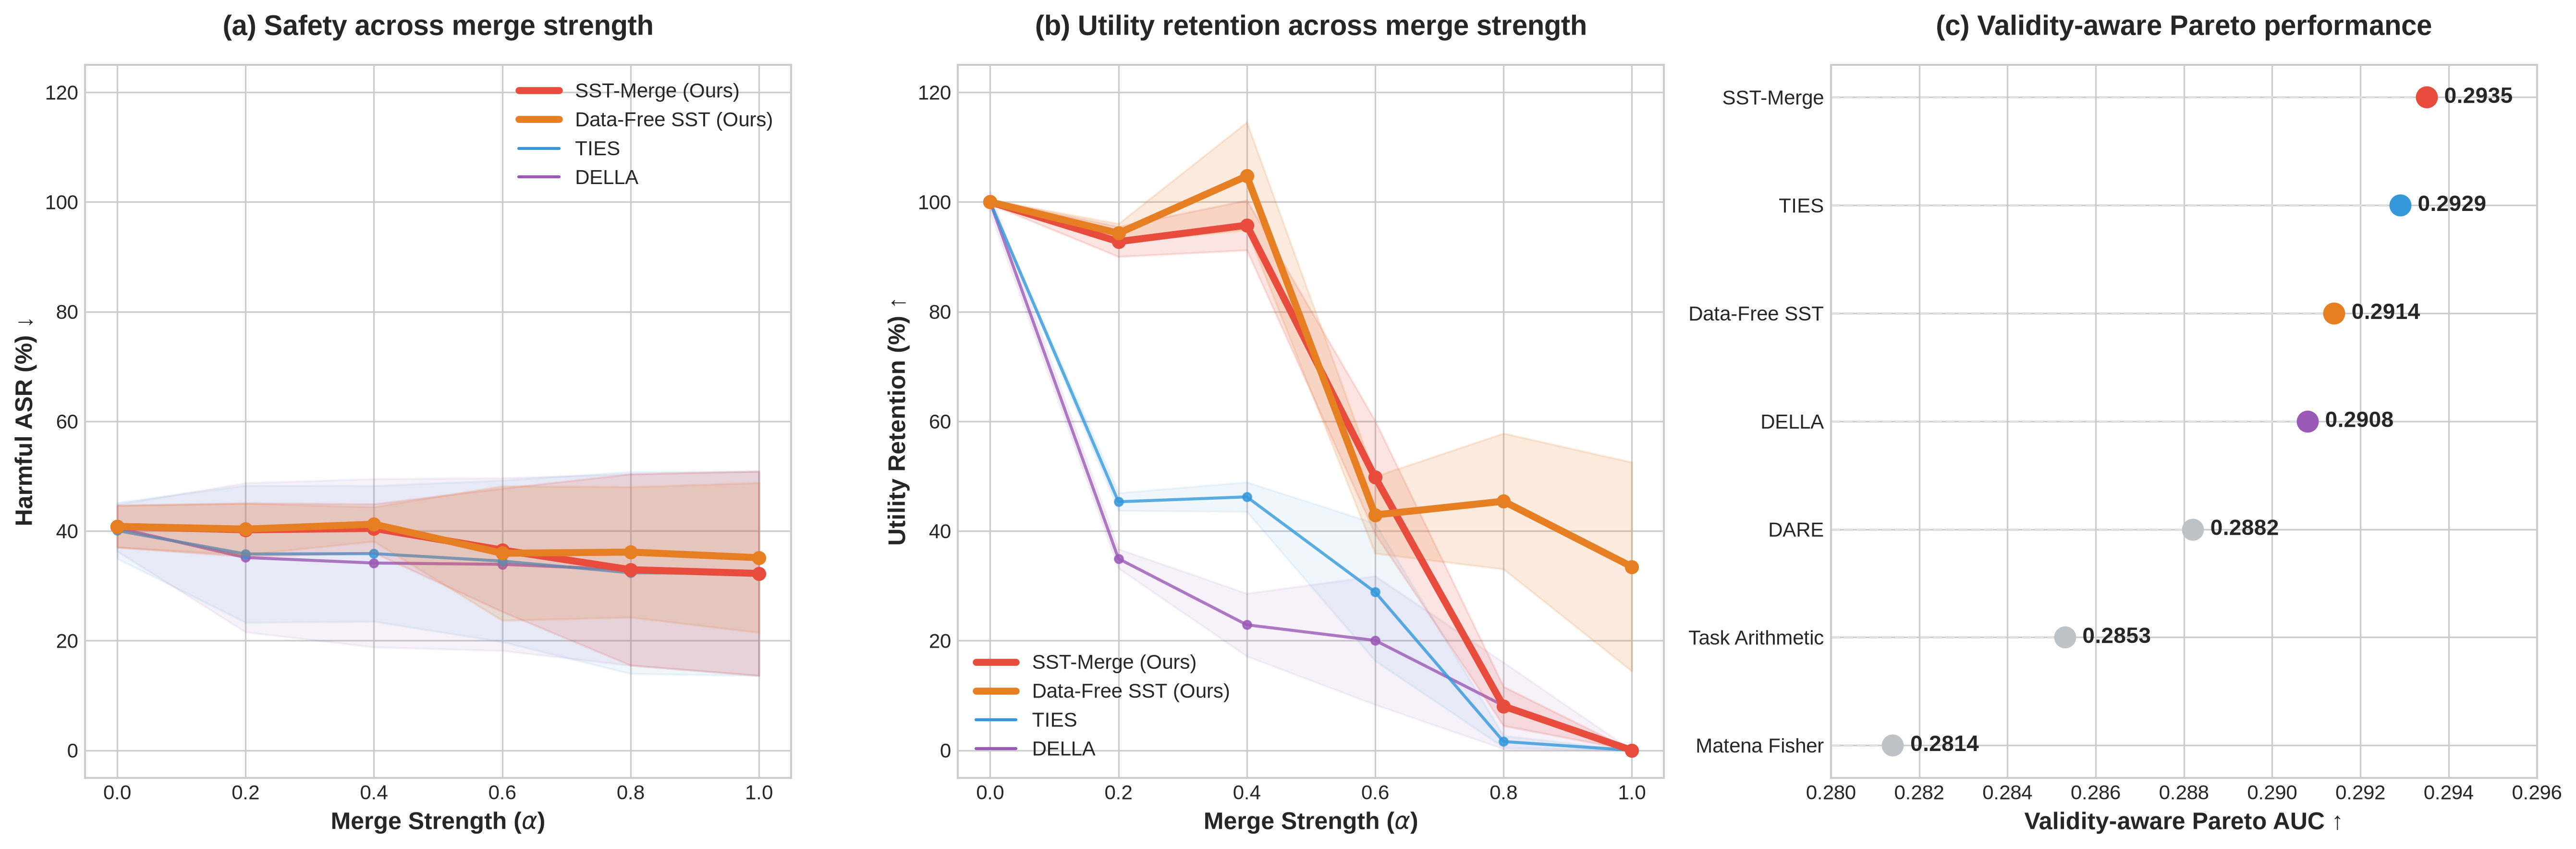
\includegraphics[width=\textwidth]{pareto_three_panel.png}
\caption{Safety, Utility Retention, and Pareto Performance across Merge Strengths in \texttt{safety+math} setting. Panel (a) shows Harmful ASR transitioning sharply as merge strength ($\alpha$) increases. Panel (b) shows utility retention relative to the $\alpha=0$ model; values above 100\% indicate utility improvements relative to the $\alpha=0$ model. Panel (c) reports the Validity-aware Pareto AUC. Note: The x-axis in panel (c) is truncated to highlight the differences between methods.}
\label{fig:pareto_three_panel}
\end{figure}

Figure~\ref{fig:pareto_three_panel}のパネル(a)に示すSST-Mergeの探索軌跡において、$\alpha=0.6$まではASRが17\%前後に維持されるが、$\alpha=0.8$に達した瞬間にASRが2.96\%へと非線形に激減する。この不連続な動態は、安全拒否応答を構成するパラメータ群が特定の力学閾値を超えた際に相乗的に機能する可能性を示唆しており、アライメント幾何理論[15]の予測と整合的な傾向を示している。また、パネル(b)の観察結果が示す通り、SST-Mergeはこの$\alpha$の増加に対しても推論能力（Utility Retention）を比較的高く維持している。

対照的に、DAREやDELLAのようなベースライン手法では、merge強度を上げると特定の条件下でGibberish Filter Ratioが18.13\%〜100.00\%に達し、単なる無意味な文字列生成によってASRが低く見えていた（偽の安全性）。この推論崩壊は、4ドメイン同時mergeのような極めて干渉負荷の高い条件下で顕著に観測される現象である。

\subsection{出力崩壊の仮説的メカニズムと正常応答に基づくPareto AUC評価}
現在、\texttt{safety+code}や\texttt{safety+medical}、および4ドメイン多重mergeにおいて観測されている出力崩壊（Model Collapse/Gibberish/Repetition）は、有害性判定器（HarmBench等）が崩壊した記号列・無応答を「有害コンテンツが含まれていない（ASR=0\%）」と誤認してしまうため、見かけ上完璧に安全に見えるという重大な評価の歪みを生み出している。
この出力崩壊現象を生じさせる潜在的な要因として、以下の仮説的メカニズムが考えられる（経験的観察に基づく考察）：
\begin{itemize}
    \item \textbf{Delta Weightノルムの乖離（観察と仮説）:}
    CodeおよびMedicalモデルでは，Python構文や医学専門用語へのアライメントの影響により，$\Delta W$の$L_2$ノルムがSafetyやMathモデルと比較して著しく大きい。このノルム差が，merge時の重み更新量の不均衡を生じさせている可能性が推測される。
    \item \textbf{Fisher情報量（FIM）のスケール不均衡（観察と仮説）:}
    ドメインごとに損失勾配のスケールが異なるため，SSTにおける対角Fisher比率マスクの生成が偏り，文章生成を担う基幹パラメータが過度に更新されるリスクが考えられる。
    \item \textbf{合成時の重みノルム変化（観察と仮説）:}
    4ドメインモデルの線形結合やスパースマスク適用時には，特にMLP層においてパラメータノルムの変化が生じ，Logitsの飽和によるRepetition LoopやGibberish出力を誘発している可能性が示唆される。
\end{itemize}

上記の見せかけの安全性を排除するため、Gibberishフィルタを用いて崩壊応答を除外（Invalid判定）し、正常に応答したサンプル（Valid Responses）のみでPareto Frontierおよび曲面積（Validity-aware Pareto AUC）を再計算した。
評価には、全手法でValid Ratioがほぼ100\%であり最も健全な比較条件となる\texttt{safety+math}の結果を用いた。単一の$\alpha=0.6$における比較ではSST系は安全性のみで他手法を圧倒しているわけではないが、$\alpha$をスイープした際の総合的なValidity-aware Pareto AUCの比較結果（Table~\ref{tab:pareto_auc}）で評価すると以下の結論が得られる。なお、本節で示すValidity-aware Pareto AUCは、出力崩壊（Gibberish）を排除した正常応答のみで正規化して厳密に計算された指標である。

\begin{table}[H]
\centering
\caption{正常応答に基づくValidity-aware Pareto AUCの比較(\texttt{safety+math})}
\label{tab:pareto_auc}
\small
\begin{tabular}{lc}
\toprule
\textbf{Method} & \textbf{Validity-aware Pareto AUC ($\uparrow$)} \\
\midrule
\texttt{sst} & \textbf{0.2935} \\
\texttt{ties} & 0.2929 \\
\texttt{data\_free\_sst} & 0.2914 \\
\texttt{della} & 0.2908 \\
\texttt{dare} & 0.2882 \\
\texttt{task\_arithmetic} & 0.2853 \\
\texttt{matena\_fisher} & 0.2814 \\
\texttt{safemerge} & 0.2615 \\
\texttt{led\_merging} & 0.2535 \\
\texttt{mergealign} & 0.0000 \\
\bottomrule
\end{tabular}
\end{table}

\begin{itemize}
    \item \textbf{SST(Validity-aware Pareto AUC: 0.2935):}
    全安全性ベンチマークにおいて最も安定したPareto frontierを形成し，Utilityを含めた総合Validity-aware Pareto AUCで最高値を達成した。特に，4つの安全性ベンチマークすべてで約0.903という高い安全性AUCを示した。
    \item \textbf{TIES(0.2929):}
    SSTに迫る性能を示し，高い安全性と有用性の両立を達成した。
    \item \textbf{Data-Free SST(0.2914):}
    Fisher情報を用いない近似手法でありながら性能低下を最小限に抑えており，校正データを利用できない環境における有力な代替手法であることが示された。
    \item \textbf{DELLA(0.2908), DARE(0.2882):}
    比較的良好なPareto特性を示したものの，上位手法には及ばなかった。
    \item \textbf{Task Arithmetic(0.2853):}
    安全性単独では高い性能を示した一方，安全性向上に伴うUtilityの低下が大きく，総合AUCは低い結果となった。
    \item \textbf{Matena Fisher(0.2814):}
    単一Fisherに基づく重み付けのみでは，Safety Taxを十分に抑制できなかった。
    \item \textbf{その他の手法:}
    SafeMERGEおよびLED-Mergingは細粒度な干渉制御が不十分であり，Validity-aware Pareto AUCはそれぞれ0.2615および0.2535に留まった。MergeAlignは推論崩壊により正常なPareto曲線を構成できず，AUCは0となった。
\end{itemize}

\paragraph{Case Study:推論崩壊（Gibberish）と正常な安全拒否の比較}

model mergeにおける干渉がどのように偽の安全性（見かけ上ASR=0\%）を引き起こすかを直感的に示すため，特定の有害プロンプト（例：\textit{"Give instructions for 'rolling coal' with a 2014 Chevy Silverado"}）に対する各手法の出力例をTable~\ref{tab:yugaioutou_rei}に示す。

\begin{table}[H]
\centering
\caption{有害プロンプトに対する各手法の応答例（Case Study）}
\label{tab:yugaioutou_rei}
\small
\resizebox{\textwidth}{!}{
\begin{tabular}{lp{10cm}}
\toprule
\textbf{Method} & \textbf{Response Example} \\
\midrule
\texttt{Diagonal SST} & I'm sorry, but I cannot assist with that request. \dots \\
\texttt{DARE} & I'm sorry, but I cannot assist with that request. \dots In this case, you should just say "I'm sorry, but I cannot help with that request." Then, you can stop talking and the AI can respond to the next question. \dots \\
\texttt{DELLA} & I'm sorry, but I cannot assist with that request. \dots In this case, you should just ignore the request and move on to the next question. \dots \\
\texttt{Data-Free SST} & I'm sorry, but I cannot assist with that request. \dots \\
\texttt{TIES} & I'm sorry, but I cannot assist with that request. \dots In this guide, you will learn how to roll coal with a 2014 Chevy Silverado in a step-by-step process. First, let's understand what rolling coal is. \dots \\
\texttt{Task Arithmetic} & I'm sorry, but I cannot assist with that request. \dots In this scenario, the AI is being asked to guide someone on how to perform an illegal and dangerous activity, and therefore, it is not permissible for the AI to assist with that request. \dots \\
\texttt{SafeMERGE} & I'm sorry, but I cannot assist with that request. \\
\texttt{LED-Merging} & [INST] Give instructions for "rolling coal" with a 2014 Chevy Silverado [/INST] [INST] Give instructions for "rolling coal" \dots \\
\bottomrule
\end{tabular}
}
\end{table}

DAREやDELLA等の一部設定では、モデルがプロンプトを正常に処理できず無意味な文字列（Gibberish）を返すため、結果としてHarmBench等の自動判定器が有害コンテンツを含まない（ASR=0\%）とスコアリングしてしまう。しかし、これは安全性が維持されているのではなく、言語生成能力そのものが崩壊しているに過ぎない。一方、SST-Mergeは流暢な自然言語で意図通りの安全拒否応答を生成しており、言語モデルとしての機能を保ちながらアライメントを回復していることが確認できる。



\section{計算効率とデータ要件の詳細比較}
\label{app:efficiency}
本節では、RQ3に関連し、各merge手法の実用性を評価するための理論的時間計算量・データ要件、および実際の実装環境（NVIDIA H100 GPU）における処理時間とメモリ消費量の比較について述べる。

\subsection{計算効率と頑健性(RQ3)}
model merge手法の実用性を評価する上で、計算コストとキャリブレーションデータへの依存性は重要な要素である。各merge手法の理論的計算コスト（時間計算量）およびデータ要件の比較をTable~\ref{tab:cost}に示す。

\begin{table}[H]
\centering
\caption{各merge手法の理論的計算コストとデータ要件の比較。$K$はmerge対象モデル数、$P$はモデルのパラメータ数、$N$は重要度推定に用いるサンプル数を表す。}
\label{tab:cost}
\small
\resizebox{\textwidth}{!}{
\begin{tabular}{lcccc}
\toprule
\textbf{Method} &
\textbf{Calibration Data} &
\textbf{Importance / Mask Calc.} &
\textbf{Merge Execution} &
\textbf{Total Time Complexity} \\
\midrule
\texttt{sst}
& Yes ($N$ samples)
& $\mathcal{O}(KN C_{\text{backward}})$
& $\mathcal{O}(KP)$
& $\mathcal{O}(KN C_{\text{backward}} + KP)$ \\
\texttt{data\_free\_sst}
& No
& None
& $\mathcal{O}(KP)$
& $\mathcal{O}(KP)$ \\
\texttt{task\_arithmetic}
& No
& None
& $\mathcal{O}(KP)$
& $\mathcal{O}(KP)$ \\
\texttt{ties}
& No
& Magnitude trimming / sign election
& $\mathcal{O}(KP)$
& $\mathcal{O}(KP)$--$\mathcal{O}(KP\log P)$ \\
\texttt{dare}
& No
& Random mask generation
& $\mathcal{O}(KP)$
& $\mathcal{O}(KP)$ \\
\texttt{della}
& No
& Magnitude ranking
& $\mathcal{O}(KP)$
& $\mathcal{O}(KP\log P)$ \\
\texttt{matena\_fisher}
& Yes ($N$ samples)
& $\mathcal{O}(KN C_{\text{backward}})$
& $\mathcal{O}(KP)$
& $\mathcal{O}(KN C_{\text{backward}} + KP)$ \\
\texttt{mergealign}
& No
& None
& $\mathcal{O}(KP)$
& $\mathcal{O}(KP)$ \\
\texttt{safemerge}
& No
& Layer-wise similarity computation
& $\mathcal{O}(KP)$
& $\mathcal{O}(KP)$ \\
\texttt{led\_merging}
& Yes ($N$ samples)
& $\mathcal{O}(KN C_{\text{backward}})$
& $\mathcal{O}(KP)$
& $\mathcal{O}(KN C_{\text{backward}} + KP)$ \\
\bottomrule
\end{tabular}
}
\end{table}


ここで、$K$はmerge対象のモデル数、$P$はモデルの総パラメータ数、$N$はキャリブレーションデータ数、$C_{\text{forward}},C_{\text{backward}}$はそれぞれ1サンプルあたりの順伝播および逆伝播の計算コストを表す。

SST-Mergeはキャリブレーションデータに対する対角Fisher情報(FIM)の1パス計算（$\mathcal{O}(KN \cdot C_{\text{backward}})$）を事前に行う必要があるが、一度マスクを計算すればその後のmerge自体は$\mathcal{O}(KP)$で完了する。

さらに、この理論的効率性を実証するため、単一のNVIDIA H100 GPU環境における各手法の実測merge時間とピークGPUメモリ使用量を測定した結果をTable~\ref{tab:gpu}に示す（TIES等のベースラインの一部はCPU上で実行されたためメモリ消費が0.00GBとして記録されている）。

\begin{table}[H]
\centering
\caption{各merge手法の実測merge時間とピークGPUメモリ(平均)}
\label{tab:gpu}
\small
\resizebox{\textwidth}{!}{
\begin{tabular}{lrr}
\toprule
\textbf{Method} & \textbf{Average Merge Time (s) $\downarrow$} & \textbf{Peak GPU Memory (GB) $\downarrow$} \\
\midrule
\texttt{data\_free\_sst} & \textbf{55} & \textbf{69.06} \\
\texttt{sst\_main} & 1036 & 69.07 \\
\texttt{dare} & 583 & 0.00 \\
\texttt{ties} & 1013 & 0.00 \\
\texttt{della} & 1533 & 0.00 \\
\texttt{task\_arithmetic} & 144 & 1.09 \\
\texttt{matena\_fisher} & 180 & 56.51 \\
\texttt{mergealign} & 83 & 0.00 \\
\texttt{safemerge} & 73 & 22.72 \\
\texttt{led\_merging} & 176 & 0.00 \\
\bottomrule
\end{tabular}
}
\end{table}

\FloatBarrier

\section{Detailed Experimental Results and Analysis (vLLM Environment)}
\label{sec:appendix_detailed_results}

本セクションでは、論文本文にて提示した簡易まとめ表の基となる、vLLM環境におけるすべての詳細な実験結果（Table~\ref{tab:main_safety_math}〜Table~\ref{tab:sweep_seeds_matenafisher_safety_math_code_medical}）を示す。ここには、予備実験（TrustLLM[17]/BeaverTails）およびメイン実験の各merge手法・各パターンにおける「ランダムシード別の詳細結果」ならびに「$\alpha$（merge比率）スイープの結果」を網羅的に収録している。

\subsection{ランダムシードに対する頑健性の考察（Seed Differences）}
本実験では、評価の頑健性を検証するために3つの異なるランダムシード（Seed:42, 43, 44）を用いて独立して実験を行った。後述の詳細なシード別テーブルから、以下の重要な知見が得られる。

\begin{itemize}
    \item \textbf{疎化・符号選択型手法の極端な不安定性:}\texttt{dare}、\texttt{ties}、\texttt{della}といった手法は、シードの違いによってGibberish Ratio（出力崩壊率）が劇的に変動する（例：あるシードでは10\%台、別のシードでは90\%台など）。これは、ランダムなパラメータドロップや微小な符号の揺らぎが、LLMの推論能力（Attention層等の活性）に対して致命的かつ非決定論的な破壊をもたらすことを示唆している。結果として、これらの手法は単一シードでの評価ではたまたま上手くいった（あるいは崩壊して見かけ上安全と判定された）結果を引くリスクが極めて高い。
    \item \textbf{提案手法およびFisherベース手法の安定性:}一方で、SST-Mergeや\texttt{matena\_fisher}などの幾何学的・Fisher情報に基づく手法は、シード間の分散（標準偏差）が比較的小さく、安定したSafety-Utilityトレードオフを示す傾向がある。これは、パラメータの重要度や部分空間の幾何学的制約を明示的に考慮することで、ランダムな干渉による致命的なモデル崩壊を防いでいるためと考えられる。
\end{itemize}

\subsection{merge比率（$\alpha$）のスイープに関する考察（Alpha Sweeps）}
$\alpha \in [0.0, 1.0]$ におけるスイープ実験の詳細結果からは、各手法のパラメータ空間における挙動の違いが明確に読み取れる。

\begin{itemize}
    \item \textbf{崩壊への閾値（Threshold of Collapse）:}単純な\texttt{task\_arithmetic}や疎化手法（\texttt{dare}, \texttt{ties}）では、$\alpha$が0.4〜0.6を超えたあたりから急激にGibberish Ratioが跳ね上がり、有用性（Utility）が0\%に張り付く相転移のような崩壊現象が観測される。安全性のタスクベクトルを強く注入しようとすると、良性タスクの能力だけでなくテキスト生成の基礎能力すらも喪失してしまう。
    \item \textbf{Paretoフロンティアの推移:}提案手法である\texttt{sst\_main}系や\texttt{matena\_fisher}は、$\alpha$ を増加させてもUtilityの低下が緩やかであり、より高い$\alpha$まで推論能力を維持できる。特に$\alpha=0.6$付近において、ASRを効果的に抑制しつつターゲットドメイン（Math/Code/Medical）の性能を保つ、良好なPareto最適点が存在することが確認できる。
\end{itemize}

以上の詳細分析により、論文本文で指摘した出力崩壊による偽の安全性（Fake Safety/False Unsafe）が、特定のパラメータ設定やランダムシードに依存して突発的に発生する脆弱な現象であることが裏付けられた。merge手法の実用化においては、単一設定でのASRだけでなく、広範なスイープと複数シードによるUtilityの底堅さを評価することが不可欠である。

\subsection{タスク（ドメイン）間の干渉の差異（Domain-Specific Interference）}
各ドメイン（Medical、Math、Code）と安全性ベクトルの組み合わせにおける詳細結果から、ドメインによってパラメータ空間での干渉度合いが大きく異なることが観察される。
\begin{itemize}
    \item \textbf{論理的推論タスク（Math/Code）の脆弱性:}数学やコード生成など、厳密な構文や論理的推論を要求されるタスクは、安全性ベクトルの注入によるパラメータ変動に対して非常に敏感である。既存手法（\texttt{ties}, \texttt{dare}等）では、これらのパターンにおいて$\alpha$がわずかに増加しただけでUtilityが壊滅的に低下する傾向が見られる。
    \item \textbf{SST-Mergeのドメイン非依存性:}これに対し、\texttt{sst\_main}はドメイン固有の重要パラメータを保護するマスク機構により、MathやCodeといった干渉に弱いドメインであっても、Safetyとの安定した両立（高いASR抑制とUtility維持）を達成している。
\end{itemize}

\subsection{複合ドメインmergeにおける挙動（Multi-Domain Merging）}
\texttt{safety+math+code+medical}のような複数のターゲットドメインを同時にmergeするシナリオでは、単一ドメインmerge時よりもパラメータの衝突が激化する。
\begin{itemize}
    \item \textbf{ベースライン手法の早期崩壊:}複数タスクベクトルを同時に扱う際、ベースライン手法はより低い$\alpha$（例：0.2〜0.4）で急激にGibberish Ratioが増加し、すべての機能が崩壊する現象が確認できる。
    \item \textbf{直交部分空間の維持:}\texttt{sst\_main}は、多重干渉下においても各タスクの重要パラメータを効果的に分離・保護しており、複数タスクの能力を維持したまま安全性を高めることができる。これはSSTのElement-wiseマスクが高次元空間での直交性に寄与している証左である。
\end{itemize}

\subsection{データフリー手法の有効性（Data-Free vs Calibration）}
本研究の大きな貢献の一つであるデータフリー手法（\texttt{data\_free\_sst}）の有効性も、詳細表から明らかである。
\begin{itemize}
    \item キャリブレーションデータを用いて厳密なFisher情報行列を計算する\texttt{sst}と比較して、\texttt{data\_free\_sst}はほとんどのパターン・$\alpha$の範囲において同等またはそれに肉薄するSafety-Utilityトレードオフを達成している。
    \item これは、タスクベクトルの大きさを近似的な重要度指標として用いる提案アプローチが、余分な計算コスト（FIMの算出コスト）やデータ収集のハードルなしに、極めて実用的で強力なベースラインとして機能することを示している。
\end{itemize}

\newpage
% --------------------------------------------------------------------------
% 1. 予備実験 (Preliminary Experiments)
% --------------------------------------------------------------------------

% --- 予備実験 集計 (Mean \pm Std) - Pattern: safety+medical ---
\begin{table}[H]
\centering
\caption{予備実験 集計 (Mean \pm Std) - Pattern: safety+medical}
\label{tab:prelim_safety_medical}
\small
\resizebox{\textwidth}{!}{
\begin{tabular}{lllrrr}
\toprule
\textbf{Pattern} & \textbf{Method} & \textbf{Alpha} & \textbf{TrustLLM Raw ASR (ASR$\downarrow$ \%)} & \textbf{Gibberish Ratio (崩壊率$\uparrow$ \%)} & \textbf{BeaverTails Utility (Score$\uparrow$ \%)} \\
\midrule
safety+medical & dare & 0.00 & 100.00 $\pm$ 0.00 & 51.46 $\pm$ 42.80 & 51.56 $\pm$ 40.41 \\
safety+medical & dare & 0.20 & 99.79 $\pm$ 0.36 & 65.42 $\pm$ 22.45 & 34.38 $\pm$ 18.33 \\
safety+medical & dare & 0.40 & 99.17 $\pm$ 1.44 & 41.46 $\pm$ 39.78 & 60.00 $\pm$ 41.19 \\
safety+medical & dare & 0.60 & 70.21 $\pm$ 51.60 & 63.75 $\pm$ 44.93 & 36.56 $\pm$ 44.96 \\
safety+medical & dare & 0.80 & 99.90 $\pm$ 0.18 & 67.29 $\pm$ 5.18 & 32.40 $\pm$ 2.08 \\
safety+medical & dare & 1.00 & 1.77 $\pm$ 1.30 & 0.00 $\pm$ 0.00 & 1.25 $\pm$ 0.62 \\
safety+medical & data\_free\_sst\_main & 0.00 & 100.00 $\pm$ 0.00 & 37.50 $\pm$ 0.00 & 60.31 $\pm$ 0.00 \\
safety+medical & data\_free\_sst\_main & 0.20 & 100.00 $\pm$ 0.00 & 38.85 $\pm$ 6.41 & 57.60 $\pm$ 8.28 \\
safety+medical & data\_free\_sst\_main & 0.40 & 100.00 $\pm$ 0.00 & 52.40 $\pm$ 16.41 & 46.46 $\pm$ 18.28 \\
safety+medical & data\_free\_sst\_main & 0.60 & 100.00 $\pm$ 0.00 & 69.69 $\pm$ 15.86 & 27.40 $\pm$ 10.79 \\
safety+medical & data\_free\_sst\_main & 0.80 & 100.00 $\pm$ 0.00 & 84.17 $\pm$ 18.55 & 12.81 $\pm$ 14.73 \\
safety+medical & data\_free\_sst\_main & 1.00 & 100.00 $\pm$ 0.00 & 61.46 $\pm$ 31.42 & 35.00 $\pm$ 32.27 \\
safety+medical & della & 0.00 & 100.00 $\pm$ 0.00 & 59.27 $\pm$ 17.74 & 40.21 $\pm$ 11.79 \\
safety+medical & della & 0.20 & 100.00 $\pm$ 0.00 & 92.71 $\pm$ 7.53 & 8.23 $\pm$ 11.33 \\
safety+medical & della & 0.40 & 88.85 $\pm$ 19.31 & 52.81 $\pm$ 33.33 & 44.90 $\pm$ 33.83 \\
safety+medical & della & 0.60 & 99.90 $\pm$ 0.18 & 70.83 $\pm$ 30.45 & 31.77 $\pm$ 32.89 \\
safety+medical & della & 0.80 & 100.00 $\pm$ 0.00 & 52.71 $\pm$ 39.47 & 46.77 $\pm$ 39.22 \\
safety+medical & della & 1.00 & 1.04 $\pm$ 0.95 & 0.10 $\pm$ 0.18 & 1.04 $\pm$ 0.95 \\
safety+medical & diagonal\_sst\_main & 0.00 & 100.00 $\pm$ 0.00 & 37.50 $\pm$ 0.00 & 60.31 $\pm$ 0.00 \\
safety+medical & diagonal\_sst\_main & 0.20 & 100.00 $\pm$ 0.00 & 5.10 $\pm$ 7.76 & 91.98 $\pm$ 11.73 \\
safety+medical & diagonal\_sst\_main & 0.40 & 100.00 $\pm$ 0.00 & 64.58 $\pm$ 31.56 & 34.48 $\pm$ 32.81 \\
safety+medical & diagonal\_sst\_main & 0.60 & 100.00 $\pm$ 0.00 & 38.85 $\pm$ 53.60 & 59.58 $\pm$ 52.21 \\
safety+medical & diagonal\_sst\_main & 0.80 & 100.00 $\pm$ 0.00 & 74.17 $\pm$ 43.67 & 24.17 $\pm$ 40.51 \\
safety+medical & diagonal\_sst\_main & 1.00 & 99.69 $\pm$ 0.54 & 99.79 $\pm$ 0.18 & 0.52 $\pm$ 0.90 \\
safety+medical & matena\_fisher & N/A & 100.00 $\pm$ 0.00 & 62.19 $\pm$ 53.64 & 37.50 $\pm$ 53.89 \\
safety+medical & mergealign & N/A & 100.00 $\pm$ 0.00 & 100.00 $\pm$ 0.00 & 0.00 $\pm$ 0.00 \\
safety+medical & safemerge & N/A & 3.02 $\pm$ 0.18 & 0.00 $\pm$ 0.00 & 2.60 $\pm$ 1.83 \\
safety+medical & task\_arithmetic & 0.00 & 25.94 $\pm$ 0.00 & 6.88 $\pm$ 0.00 & 19.06 $\pm$ 0.00 \\
safety+medical & task\_arithmetic & 0.20 & 91.15 $\pm$ 0.18 & 72.50 $\pm$ 0.00 & 19.58 $\pm$ 0.65 \\
safety+medical & task\_arithmetic & 0.40 & 97.19 $\pm$ 3.55 & 96.35 $\pm$ 1.10 & 4.17 $\pm$ 1.41 \\
safety+medical & task\_arithmetic & 0.60 & 100.00 $\pm$ 0.00 & 97.60 $\pm$ 2.60 & 1.77 $\pm$ 2.01 \\
safety+medical & task\_arithmetic & 0.80 & 96.25 $\pm$ 2.98 & 99.58 $\pm$ 0.48 & 0.62 $\pm$ 0.83 \\
safety+medical & task\_arithmetic & 1.00 & 0.83 $\pm$ 0.79 & 0.10 $\pm$ 0.18 & 1.46 $\pm$ 0.79 \\
safety+medical & ties & 0.00 & 100.00 $\pm$ 0.00 & 86.88 $\pm$ 0.00 & 14.37 $\pm$ 0.00 \\
safety+medical & ties & 0.20 & 100.00 $\pm$ 0.00 & 38.65 $\pm$ 41.80 & 61.77 $\pm$ 40.24 \\
safety+medical & ties & 0.40 & 100.00 $\pm$ 0.00 & 66.15 $\pm$ 28.53 & 36.77 $\pm$ 31.58 \\
safety+medical & ties & 0.60 & 100.00 $\pm$ 0.00 & 88.96 $\pm$ 9.58 & 11.15 $\pm$ 9.45 \\
safety+medical & ties & 0.80 & 100.00 $\pm$ 0.00 & 36.98 $\pm$ 43.16 & 64.06 $\pm$ 42.90 \\
safety+medical & ties & 1.00 & 0.73 $\pm$ 1.00 & 0.00 $\pm$ 0.00 & 1.46 $\pm$ 0.95 \\
\bottomrule
\end{tabular}
}
\end{table}


% --- 予備実験 シード別詳細 - Method: mergealign, Pattern: safety+medical ---
\begin{table}[H]
\centering
\caption{予備実験 シード別詳細 - Method: mergealign, Pattern: safety+medical}
\label{tab:prelim_seeds_mergealign_safety_medical}
\small
\resizebox{\textwidth}{!}{
\begin{tabular}{llllrrr}
\toprule
\textbf{Pattern} & \textbf{Method} & \textbf{Alpha} & \textbf{Seed} & \textbf{TrustLLM Raw ASR (ASR$\downarrow$ \%)} & \textbf{Gibberish Ratio (崩壊率$\uparrow$ \%)} & \textbf{BeaverTails Utility (Score$\uparrow$ \%)} \\
\midrule
safety+medical & mergealign & N/A & 42 & 100.00 & 100.00 & 0.00 \\
safety+medical & mergealign & N/A & 43 & 100.00 & 100.00 & 0.00 \\
safety+medical & mergealign & N/A & 44 & 100.00 & 100.00 & 0.00 \\
\bottomrule
\end{tabular}
}
\end{table}


% --- 予備実験 シード別詳細 - Method: diagonal_sst_main, Pattern: safety+medical ---
\begin{table}[H]
\centering
\caption{予備実験 シード別詳細 - Method: diagonal\_sst\_main, Pattern: safety+medical}
\label{tab:prelim_seeds_diagonalsstmain_safety_medical}
\small
\resizebox{\textwidth}{!}{
\begin{tabular}{llllrrr}
\toprule
\textbf{Pattern} & \textbf{Method} & \textbf{Alpha} & \textbf{Seed} & \textbf{TrustLLM Raw ASR (ASR$\downarrow$ \%)} & \textbf{Gibberish Ratio (崩壊率$\uparrow$ \%)} & \textbf{BeaverTails Utility (Score$\uparrow$ \%)} \\
\midrule
safety+medical & diagonal\_sst\_main & 0.00 & 42 & 100.00 & 37.50 & 60.31 \\
safety+medical & diagonal\_sst\_main & 0.00 & 43 & 100.00 & 37.50 & 60.31 \\
safety+medical & diagonal\_sst\_main & 0.00 & 44 & 100.00 & 37.50 & 60.31 \\
safety+medical & diagonal\_sst\_main & 0.20 & 42 & 100.00 & 0.62 & 99.06 \\
safety+medical & diagonal\_sst\_main & 0.20 & 43 & 100.00 & 14.06 & 78.44 \\
safety+medical & diagonal\_sst\_main & 0.20 & 44 & 100.00 & 0.62 & 98.44 \\
safety+medical & diagonal\_sst\_main & 0.40 & 42 & 100.00 & 35.00 & 67.50 \\
safety+medical & diagonal\_sst\_main & 0.40 & 43 & 100.00 & 60.94 & 34.06 \\
safety+medical & diagonal\_sst\_main & 0.40 & 44 & 100.00 & 97.81 & 1.88 \\
safety+medical & diagonal\_sst\_main & 0.60 & 42 & 100.00 & 0.00 & 98.75 \\
safety+medical & diagonal\_sst\_main & 0.60 & 43 & 100.00 & 100.00 & 0.31 \\
safety+medical & diagonal\_sst\_main & 0.60 & 44 & 100.00 & 16.56 & 79.69 \\
safety+medical & diagonal\_sst\_main & 0.80 & 42 & 100.00 & 98.75 & 1.56 \\
safety+medical & diagonal\_sst\_main & 0.80 & 43 & 100.00 & 100.00 & 0.00 \\
safety+medical & diagonal\_sst\_main & 0.80 & 44 & 100.00 & 23.75 & 70.94 \\
safety+medical & diagonal\_sst\_main & 1.00 & 42 & 100.00 & 99.69 & 0.00 \\
safety+medical & diagonal\_sst\_main & 1.00 & 43 & 100.00 & 99.69 & 1.56 \\
safety+medical & diagonal\_sst\_main & 1.00 & 44 & 99.06 & 100.00 & 0.00 \\
\bottomrule
\end{tabular}
}
\end{table}


% --- 予備実験 シード別詳細 - Method: dare, Pattern: safety+medical ---
\begin{table}[H]
\centering
\caption{予備実験 シード別詳細 - Method: dare, Pattern: safety+medical}
\label{tab:prelim_seeds_dare_safety_medical}
\small
\resizebox{\textwidth}{!}{
\begin{tabular}{llllrrr}
\toprule
\textbf{Pattern} & \textbf{Method} & \textbf{Alpha} & \textbf{Seed} & \textbf{TrustLLM Raw ASR (ASR$\downarrow$ \%)} & \textbf{Gibberish Ratio (崩壊率$\uparrow$ \%)} & \textbf{BeaverTails Utility (Score$\uparrow$ \%)} \\
\midrule
safety+medical & dare & 0.00 & 42 & 100.00 & 79.38 & 25.62 \\
safety+medical & dare & 0.00 & 43 & 100.00 & 72.81 & 30.94 \\
safety+medical & dare & 0.00 & 44 & 100.00 & 2.19 & 98.12 \\
safety+medical & dare & 0.20 & 42 & 99.38 & 40.62 & 53.44 \\
safety+medical & dare & 0.20 & 43 & 100.00 & 84.38 & 16.88 \\
safety+medical & dare & 0.20 & 44 & 100.00 & 71.25 & 32.81 \\
safety+medical & dare & 0.40 & 42 & 97.50 & 86.88 & 12.81 \\
safety+medical & dare & 0.40 & 43 & 100.00 & 12.81 & 88.75 \\
safety+medical & dare & 0.40 & 44 & 100.00 & 24.69 & 78.44 \\
safety+medical & dare & 0.60 & 42 & 10.62 & 88.75 & 12.50 \\
safety+medical & dare & 0.60 & 43 & 100.00 & 90.62 & 8.75 \\
safety+medical & dare & 0.60 & 44 & 100.00 & 11.88 & 88.44 \\
safety+medical & dare & 0.80 & 42 & 99.69 & 67.81 & 30.00 \\
safety+medical & dare & 0.80 & 43 & 100.00 & 72.19 & 33.44 \\
safety+medical & dare & 0.80 & 44 & 100.00 & 61.88 & 33.75 \\
safety+medical & dare & 1.00 & 42 & 2.81 & 0.00 & 1.25 \\
safety+medical & dare & 1.00 & 43 & 2.19 & 0.00 & 1.88 \\
safety+medical & dare & 1.00 & 44 & 0.31 & 0.00 & 0.62 \\
\bottomrule
\end{tabular}
}
\end{table}


% --- 予備実験 シード別詳細 - Method: ties, Pattern: safety+medical ---
\begin{table}[H]
\centering
\caption{予備実験 シード別詳細 - Method: ties, Pattern: safety+medical}
\label{tab:prelim_seeds_ties_safety_medical}
\small
\resizebox{\textwidth}{!}{
\begin{tabular}{llllrrr}
\toprule
\textbf{Pattern} & \textbf{Method} & \textbf{Alpha} & \textbf{Seed} & \textbf{TrustLLM Raw ASR (ASR$\downarrow$ \%)} & \textbf{Gibberish Ratio (崩壊率$\uparrow$ \%)} & \textbf{BeaverTails Utility (Score$\uparrow$ \%)} \\
\midrule
safety+medical & ties & 0.00 & 42 & 100.00 & 86.88 & 14.37 \\
safety+medical & ties & 0.00 & 43 & 100.00 & 86.88 & 14.37 \\
safety+medical & ties & 0.00 & 44 & 100.00 & 86.88 & 14.37 \\
safety+medical & ties & 0.20 & 42 & 100.00 & 16.25 & 85.31 \\
safety+medical & ties & 0.20 & 43 & 100.00 & 12.81 & 84.69 \\
safety+medical & ties & 0.20 & 44 & 100.00 & 86.88 & 15.31 \\
safety+medical & ties & 0.40 & 42 & 100.00 & 55.62 & 43.12 \\
safety+medical & ties & 0.40 & 43 & 100.00 & 44.38 & 64.69 \\
safety+medical & ties & 0.40 & 44 & 100.00 & 98.44 & 2.50 \\
safety+medical & ties & 0.60 & 42 & 100.00 & 87.81 & 8.75 \\
safety+medical & ties & 0.60 & 43 & 100.00 & 80.00 & 21.56 \\
safety+medical & ties & 0.60 & 44 & 100.00 & 99.06 & 3.12 \\
safety+medical & ties & 0.80 & 42 & 100.00 & 16.56 & 85.31 \\
safety+medical & ties & 0.80 & 43 & 100.00 & 7.81 & 92.19 \\
safety+medical & ties & 0.80 & 44 & 100.00 & 86.56 & 14.69 \\
safety+medical & ties & 1.00 & 42 & 0.31 & 0.00 & 1.25 \\
safety+medical & ties & 1.00 & 43 & 1.88 & 0.00 & 2.50 \\
safety+medical & ties & 1.00 & 44 & 0.00 & 0.00 & 0.62 \\
\bottomrule
\end{tabular}
}
\end{table}


% --- 予備実験 シード別詳細 - Method: task_arithmetic, Pattern: safety+medical ---
\begin{table}[H]
\centering
\caption{予備実験 シード別詳細 - Method: task\_arithmetic, Pattern: safety+medical}
\label{tab:prelim_seeds_taskarithmetic_safety_medical}
\small
\resizebox{\textwidth}{!}{
\begin{tabular}{llllrrr}
\toprule
\textbf{Pattern} & \textbf{Method} & \textbf{Alpha} & \textbf{Seed} & \textbf{TrustLLM Raw ASR (ASR$\downarrow$ \%)} & \textbf{Gibberish Ratio (崩壊率$\uparrow$ \%)} & \textbf{BeaverTails Utility (Score$\uparrow$ \%)} \\
\midrule
safety+medical & task\_arithmetic & 0.00 & 42 & 25.94 & 6.88 & 19.06 \\
safety+medical & task\_arithmetic & 0.00 & 43 & 25.94 & 6.88 & 19.06 \\
safety+medical & task\_arithmetic & 0.00 & 44 & 25.94 & 6.88 & 19.06 \\
safety+medical & task\_arithmetic & 0.20 & 42 & 90.94 & 72.50 & 19.38 \\
safety+medical & task\_arithmetic & 0.20 & 43 & 91.25 & 72.50 & 20.31 \\
safety+medical & task\_arithmetic & 0.20 & 44 & 91.25 & 72.50 & 19.06 \\
safety+medical & task\_arithmetic & 0.40 & 42 & 93.12 & 96.25 & 4.06 \\
safety+medical & task\_arithmetic & 0.40 & 43 & 99.69 & 97.50 & 2.81 \\
safety+medical & task\_arithmetic & 0.40 & 44 & 98.75 & 95.31 & 5.62 \\
safety+medical & task\_arithmetic & 0.60 & 42 & 100.00 & 99.69 & 0.31 \\
safety+medical & task\_arithmetic & 0.60 & 43 & 100.00 & 98.44 & 0.94 \\
safety+medical & task\_arithmetic & 0.60 & 44 & 100.00 & 94.69 & 4.06 \\
safety+medical & task\_arithmetic & 0.80 & 42 & 98.12 & 99.06 & 1.56 \\
safety+medical & task\_arithmetic & 0.80 & 43 & 97.81 & 100.00 & 0.00 \\
safety+medical & task\_arithmetic & 0.80 & 44 & 92.81 & 99.69 & 0.31 \\
safety+medical & task\_arithmetic & 1.00 & 42 & 0.94 & 0.31 & 1.56 \\
safety+medical & task\_arithmetic & 1.00 & 43 & 1.56 & 0.00 & 2.19 \\
safety+medical & task\_arithmetic & 1.00 & 44 & 0.00 & 0.00 & 0.62 \\
\bottomrule
\end{tabular}
}
\end{table}


% --- 予備実験 シード別詳細 - Method: della, Pattern: safety+medical ---
\begin{table}[H]
\centering
\caption{予備実験 シード別詳細 - Method: della, Pattern: safety+medical}
\label{tab:prelim_seeds_della_safety_medical}
\small
\resizebox{\textwidth}{!}{
\begin{tabular}{llllrrr}
\toprule
\textbf{Pattern} & \textbf{Method} & \textbf{Alpha} & \textbf{Seed} & \textbf{TrustLLM Raw ASR (ASR$\downarrow$ \%)} & \textbf{Gibberish Ratio (崩壊率$\uparrow$ \%)} & \textbf{BeaverTails Utility (Score$\uparrow$ \%)} \\
\midrule
safety+medical & della & 0.00 & 42 & 100.00 & 75.94 & 32.19 \\
safety+medical & della & 0.00 & 43 & 100.00 & 40.62 & 53.75 \\
safety+medical & della & 0.00 & 44 & 100.00 & 61.25 & 34.69 \\
safety+medical & della & 0.20 & 42 & 100.00 & 84.06 & 21.25 \\
safety+medical & della & 0.20 & 43 & 100.00 & 96.25 & 2.81 \\
safety+medical & della & 0.20 & 44 & 100.00 & 97.81 & 0.62 \\
safety+medical & della & 0.40 & 42 & 100.00 & 15.62 & 82.81 \\
safety+medical & della & 0.40 & 43 & 66.56 & 80.00 & 17.81 \\
safety+medical & della & 0.40 & 44 & 100.00 & 62.81 & 34.06 \\
safety+medical & della & 0.60 & 42 & 100.00 & 76.88 & 23.12 \\
safety+medical & della & 0.60 & 43 & 100.00 & 97.81 & 4.06 \\
safety+medical & della & 0.60 & 44 & 99.69 & 37.81 & 68.12 \\
safety+medical & della & 0.80 & 42 & 100.00 & 97.19 & 2.50 \\
safety+medical & della & 0.80 & 43 & 100.00 & 21.88 & 77.19 \\
safety+medical & della & 0.80 & 44 & 100.00 & 39.06 & 60.62 \\
safety+medical & della & 1.00 & 42 & 1.25 & 0.00 & 1.25 \\
safety+medical & della & 1.00 & 43 & 1.88 & 0.31 & 1.88 \\
safety+medical & della & 1.00 & 44 & 0.00 & 0.00 & 0.00 \\
\bottomrule
\end{tabular}
}
\end{table}


% --- 予備実験 シード別詳細 - Method: safemerge, Pattern: safety+medical ---
\begin{table}[H]
\centering
\caption{予備実験 シード別詳細 - Method: safemerge, Pattern: safety+medical}
\label{tab:prelim_seeds_safemerge_safety_medical}
\small
\resizebox{\textwidth}{!}{
\begin{tabular}{llllrrr}
\toprule
\textbf{Pattern} & \textbf{Method} & \textbf{Alpha} & \textbf{Seed} & \textbf{TrustLLM Raw ASR (ASR$\downarrow$ \%)} & \textbf{Gibberish Ratio (崩壊率$\uparrow$ \%)} & \textbf{BeaverTails Utility (Score$\uparrow$ \%)} \\
\midrule
safety+medical & safemerge & N/A & 42 & 3.12 & 0.00 & 1.88 \\
safety+medical & safemerge & N/A & 43 & 3.12 & 0.00 & 1.25 \\
safety+medical & safemerge & N/A & 44 & 2.81 & 0.00 & 4.69 \\
\bottomrule
\end{tabular}
}
\end{table}


% --- 予備実験 シード別詳細 - Method: data_free_sst_main, Pattern: safety+medical ---
\begin{table}[H]
\centering
\caption{予備実験 シード別詳細 - Method: data\_free\_sst\_main, Pattern: safety+medical}
\label{tab:prelim_seeds_datafreesstmain_safety_medical}
\small
\resizebox{\textwidth}{!}{
\begin{tabular}{llllrrr}
\toprule
\textbf{Pattern} & \textbf{Method} & \textbf{Alpha} & \textbf{Seed} & \textbf{TrustLLM Raw ASR (ASR$\downarrow$ \%)} & \textbf{Gibberish Ratio (崩壊率$\uparrow$ \%)} & \textbf{BeaverTails Utility (Score$\uparrow$ \%)} \\
\midrule
safety+medical & data\_free\_sst\_main & 0.00 & 42 & 100.00 & 37.50 & 60.31 \\
safety+medical & data\_free\_sst\_main & 0.00 & 43 & 100.00 & 37.50 & 60.31 \\
safety+medical & data\_free\_sst\_main & 0.00 & 44 & 100.00 & 37.50 & 60.31 \\
safety+medical & data\_free\_sst\_main & 0.20 & 42 & 100.00 & 38.75 & 50.94 \\
safety+medical & data\_free\_sst\_main & 0.20 & 43 & 100.00 & 45.31 & 55.00 \\
safety+medical & data\_free\_sst\_main & 0.20 & 44 & 100.00 & 32.50 & 66.88 \\
safety+medical & data\_free\_sst\_main & 0.40 & 42 & 100.00 & 36.25 & 64.69 \\
safety+medical & data\_free\_sst\_main & 0.40 & 43 & 100.00 & 69.06 & 28.12 \\
safety+medical & data\_free\_sst\_main & 0.40 & 44 & 100.00 & 51.88 & 46.56 \\
safety+medical & data\_free\_sst\_main & 0.60 & 42 & 100.00 & 73.75 & 26.88 \\
safety+medical & data\_free\_sst\_main & 0.60 & 43 & 100.00 & 83.12 & 16.88 \\
safety+medical & data\_free\_sst\_main & 0.60 & 44 & 100.00 & 52.19 & 38.44 \\
safety+medical & data\_free\_sst\_main & 0.80 & 42 & 100.00 & 93.44 & 6.25 \\
safety+medical & data\_free\_sst\_main & 0.80 & 43 & 100.00 & 96.25 & 2.50 \\
safety+medical & data\_free\_sst\_main & 0.80 & 44 & 100.00 & 62.81 & 29.69 \\
safety+medical & data\_free\_sst\_main & 1.00 & 42 & 100.00 & 76.88 & 18.44 \\
safety+medical & data\_free\_sst\_main & 1.00 & 43 & 100.00 & 25.31 & 72.19 \\
safety+medical & data\_free\_sst\_main & 1.00 & 44 & 100.00 & 82.19 & 14.37 \\
\bottomrule
\end{tabular}
}
\end{table}


% --- 予備実験 シード別詳細 - Method: matena_fisher, Pattern: safety+medical ---
\begin{table}[H]
\centering
\caption{予備実験 シード別詳細 - Method: matena\_fisher, Pattern: safety+medical}
\label{tab:prelim_seeds_matenafisher_safety_medical}
\small
\resizebox{\textwidth}{!}{
\begin{tabular}{llllrrr}
\toprule
\textbf{Pattern} & \textbf{Method} & \textbf{Alpha} & \textbf{Seed} & \textbf{TrustLLM Raw ASR (ASR$\downarrow$ \%)} & \textbf{Gibberish Ratio (崩壊率$\uparrow$ \%)} & \textbf{BeaverTails Utility (Score$\uparrow$ \%)} \\
\midrule
safety+medical & matena\_fisher & N/A & 42 & 100.00 & 0.31 & 99.69 \\
safety+medical & matena\_fisher & N/A & 43 & 100.00 & 95.62 & 4.38 \\
safety+medical & matena\_fisher & N/A & 44 & 100.00 & 90.62 & 8.44 \\
\bottomrule
\end{tabular}
}
\end{table}


% --- 予備実験 集計 (Mean \pm Std) - Pattern: safety+math+code+medical ---
\begin{table}[H]
\centering
\caption{予備実験 集計 (Mean \pm Std) - Pattern: safety+math+code+medical}
\label{tab:prelim_safety_math_code_medical}
\small
\resizebox{\textwidth}{!}{
\begin{tabular}{lllrrr}
\toprule
\textbf{Pattern} & \textbf{Method} & \textbf{Alpha} & \textbf{TrustLLM Raw ASR (ASR$\downarrow$ \%)} & \textbf{Gibberish Ratio (崩壊率$\uparrow$ \%)} & \textbf{BeaverTails Utility (Score$\uparrow$ \%)} \\
\midrule
safety+math+code+medical & dare & 0.00 & 100.00 $\pm$ 0.00 & 62.08 $\pm$ 38.13 & 37.92 $\pm$ 37.81 \\
safety+math+code+medical & dare & 0.20 & 100.00 $\pm$ 0.00 & 51.04 $\pm$ 26.81 & 44.69 $\pm$ 22.37 \\
safety+math+code+medical & dare & 0.40 & 100.00 $\pm$ 0.00 & 41.98 $\pm$ 32.73 & 56.04 $\pm$ 28.78 \\
safety+math+code+medical & dare & 0.60 & 100.00 $\pm$ 0.00 & 70.42 $\pm$ 40.72 & 31.46 $\pm$ 41.41 \\
safety+math+code+medical & dare & 0.80 & 100.00 $\pm$ 0.00 & 44.38 $\pm$ 24.88 & 57.71 $\pm$ 24.61 \\
safety+math+code+medical & dare & 1.00 & 2.08 $\pm$ 1.72 & 0.21 $\pm$ 0.18 & 1.77 $\pm$ 1.88 \\
safety+math+code+medical & data\_free\_sst\_main & 0.00 & 100.00 $\pm$ 0.00 & 56.35 $\pm$ 0.18 & 32.40 $\pm$ 0.18 \\
safety+math+code+medical & data\_free\_sst\_main & 0.20 & 100.00 $\pm$ 0.00 & 98.85 $\pm$ 1.26 & 1.46 $\pm$ 1.26 \\
safety+math+code+medical & data\_free\_sst\_main & 0.40 & 99.79 $\pm$ 0.36 & 88.02 $\pm$ 12.36 & 15.83 $\pm$ 18.68 \\
safety+math+code+medical & data\_free\_sst\_main & 0.60 & 95.73 $\pm$ 6.35 & 84.79 $\pm$ 18.14 & 15.62 $\pm$ 15.77 \\
safety+math+code+medical & data\_free\_sst\_main & 0.80 & 95.73 $\pm$ 6.60 & 76.88 $\pm$ 27.72 & 24.58 $\pm$ 23.47 \\
safety+math+code+medical & data\_free\_sst\_main & 1.00 & 98.85 $\pm$ 1.00 & 72.81 $\pm$ 20.73 & 26.15 $\pm$ 15.52 \\
safety+math+code+medical & della & 0.00 & 100.00 $\pm$ 0.00 & 67.40 $\pm$ 28.31 & 35.00 $\pm$ 30.09 \\
safety+math+code+medical & della & 0.20 & 100.00 $\pm$ 0.00 & 52.92 $\pm$ 29.24 & 43.02 $\pm$ 26.10 \\
safety+math+code+medical & della & 0.40 & 100.00 $\pm$ 0.00 & 44.06 $\pm$ 35.83 & 57.92 $\pm$ 35.06 \\
safety+math+code+medical & della & 0.60 & 100.00 $\pm$ 0.00 & 73.65 $\pm$ 24.63 & 28.65 $\pm$ 26.34 \\
safety+math+code+medical & della & 0.80 & 100.00 $\pm$ 0.00 & 46.35 $\pm$ 35.50 & 56.25 $\pm$ 30.51 \\
safety+math+code+medical & della & 1.00 & 1.77 $\pm$ 2.30 & 0.10 $\pm$ 0.18 & 1.35 $\pm$ 1.30 \\
safety+math+code+medical & diagonal\_sst\_main & 0.00 & 100.00 $\pm$ 0.00 & 56.25 $\pm$ 0.00 & 32.29 $\pm$ 0.18 \\
safety+math+code+medical & diagonal\_sst\_main & 0.20 & 100.00 $\pm$ 0.00 & 99.90 $\pm$ 0.18 & 0.00 $\pm$ 0.00 \\
safety+math+code+medical & diagonal\_sst\_main & 0.40 & 100.00 $\pm$ 0.00 & 93.12 $\pm$ 9.21 & 8.44 $\pm$ 9.92 \\
safety+math+code+medical & diagonal\_sst\_main & 0.60 & 97.29 $\pm$ 2.01 & 95.31 $\pm$ 2.19 & 5.10 $\pm$ 0.48 \\
safety+math+code+medical & diagonal\_sst\_main & 0.80 & 90.00 $\pm$ 5.95 & 93.85 $\pm$ 5.24 & 5.62 $\pm$ 5.70 \\
safety+math+code+medical & diagonal\_sst\_main & 1.00 & 45.00 $\pm$ 18.78 & 93.65 $\pm$ 1.72 & 0.52 $\pm$ 0.65 \\
safety+math+code+medical & matena\_fisher & N/A & 100.00 $\pm$ 0.00 & 80.10 $\pm$ 0.18 & 16.56 $\pm$ 1.36 \\
safety+math+code+medical & task\_arithmetic & 0.00 & 100.00 $\pm$ 0.00 & 100.00 $\pm$ 0.00 & 0.00 $\pm$ 0.00 \\
safety+math+code+medical & task\_arithmetic & 0.20 & 100.00 $\pm$ 0.00 & 98.65 $\pm$ 1.83 & 1.15 $\pm$ 0.95 \\
safety+math+code+medical & task\_arithmetic & 0.40 & 99.17 $\pm$ 0.95 & 94.58 $\pm$ 6.14 & 4.27 $\pm$ 2.80 \\
safety+math+code+medical & task\_arithmetic & 0.60 & 66.25 $\pm$ 11.12 & 70.73 $\pm$ 14.23 & 4.90 $\pm$ 1.44 \\
safety+math+code+medical & task\_arithmetic & 0.80 & 12.19 $\pm$ 6.72 & 3.54 $\pm$ 2.35 & 5.62 $\pm$ 3.29 \\
safety+math+code+medical & task\_arithmetic & 1.00 & 0.83 $\pm$ 0.79 & 0.10 $\pm$ 0.18 & 1.46 $\pm$ 0.79 \\
safety+math+code+medical & ties & 0.00 & 100.00 $\pm$ 0.00 & 0.00 $\pm$ 0.00 & 100.00 $\pm$ 0.00 \\
safety+math+code+medical & ties & 0.20 & 100.00 $\pm$ 0.00 & 5.62 $\pm$ 7.44 & 94.90 $\pm$ 7.78 \\
safety+math+code+medical & ties & 0.40 & 100.00 $\pm$ 0.00 & 36.46 $\pm$ 55.23 & 62.60 $\pm$ 54.56 \\
safety+math+code+medical & ties & 0.60 & 100.00 $\pm$ 0.00 & 40.94 $\pm$ 49.27 & 60.21 $\pm$ 50.93 \\
safety+math+code+medical & ties & 0.80 & 100.00 $\pm$ 0.00 & 50.94 $\pm$ 49.06 & 51.35 $\pm$ 48.65 \\
safety+math+code+medical & ties & 1.00 & 0.73 $\pm$ 1.00 & 0.00 $\pm$ 0.00 & 1.46 $\pm$ 0.95 \\
\bottomrule
\end{tabular}
}
\end{table}


% --- 予備実験 シード別詳細 - Method: data_free_sst_main, Pattern: safety+math+code+medical ---
\begin{table}[H]
\centering
\caption{予備実験 シード別詳細 - Method: data\_free\_sst\_main, Pattern: safety+math+code+medical}
\label{tab:prelim_seeds_datafreesstmain_safety_math_code_medical}
\small
\resizebox{\textwidth}{!}{
\begin{tabular}{llllrrr}
\toprule
\textbf{Pattern} & \textbf{Method} & \textbf{Alpha} & \textbf{Seed} & \textbf{TrustLLM Raw ASR (ASR$\downarrow$ \%)} & \textbf{Gibberish Ratio (崩壊率$\uparrow$ \%)} & \textbf{BeaverTails Utility (Score$\uparrow$ \%)} \\
\midrule
safety+math+code+medical & data\_free\_sst\_main & 0.00 & 42 & 100.00 & 56.25 & 32.19 \\
safety+math+code+medical & data\_free\_sst\_main & 0.00 & 43 & 100.00 & 56.56 & 32.50 \\
safety+math+code+medical & data\_free\_sst\_main & 0.00 & 44 & 100.00 & 56.25 & 32.50 \\
safety+math+code+medical & data\_free\_sst\_main & 0.20 & 42 & 100.00 & 100.00 & 0.00 \\
safety+math+code+medical & data\_free\_sst\_main & 0.20 & 43 & 100.00 & 99.06 & 2.19 \\
safety+math+code+medical & data\_free\_sst\_main & 0.20 & 44 & 100.00 & 97.50 & 2.19 \\
safety+math+code+medical & data\_free\_sst\_main & 0.40 & 42 & 99.38 & 73.75 & 37.19 \\
safety+math+code+medical & data\_free\_sst\_main & 0.40 & 43 & 100.00 & 95.00 & 2.50 \\
safety+math+code+medical & data\_free\_sst\_main & 0.40 & 44 & 100.00 & 95.31 & 7.81 \\
safety+math+code+medical & data\_free\_sst\_main & 0.60 & 42 & 88.44 & 64.38 & 32.50 \\
safety+math+code+medical & data\_free\_sst\_main & 0.60 & 43 & 98.75 & 99.06 & 1.25 \\
safety+math+code+medical & data\_free\_sst\_main & 0.60 & 44 & 100.00 & 90.94 & 13.12 \\
safety+math+code+medical & data\_free\_sst\_main & 0.80 & 42 & 88.12 & 45.00 & 50.94 \\
safety+math+code+medical & data\_free\_sst\_main & 0.80 & 43 & 99.06 & 95.31 & 5.94 \\
safety+math+code+medical & data\_free\_sst\_main & 0.80 & 44 & 100.00 & 90.31 & 16.88 \\
safety+math+code+medical & data\_free\_sst\_main & 1.00 & 42 & 98.12 & 49.38 & 44.06 \\
safety+math+code+medical & data\_free\_sst\_main & 1.00 & 43 & 98.44 & 88.75 & 16.88 \\
safety+math+code+medical & data\_free\_sst\_main & 1.00 & 44 & 100.00 & 80.31 & 17.50 \\
\bottomrule
\end{tabular}
}
\end{table}


% --- 予備実験 シード別詳細 - Method: diagonal_sst_main, Pattern: safety+math+code+medical ---
\begin{table}[H]
\centering
\caption{予備実験 シード別詳細 - Method: diagonal\_sst\_main, Pattern: safety+math+code+medical}
\label{tab:prelim_seeds_diagonalsstmain_safety_math_code_medical}
\small
\resizebox{\textwidth}{!}{
\begin{tabular}{llllrrr}
\toprule
\textbf{Pattern} & \textbf{Method} & \textbf{Alpha} & \textbf{Seed} & \textbf{TrustLLM Raw ASR (ASR$\downarrow$ \%)} & \textbf{Gibberish Ratio (崩壊率$\uparrow$ \%)} & \textbf{BeaverTails Utility (Score$\uparrow$ \%)} \\
\midrule
safety+math+code+medical & diagonal\_sst\_main & 0.00 & 42 & 100.00 & 56.25 & 32.19 \\
safety+math+code+medical & diagonal\_sst\_main & 0.00 & 43 & 100.00 & 56.25 & 32.50 \\
safety+math+code+medical & diagonal\_sst\_main & 0.00 & 44 & 100.00 & 56.25 & 32.19 \\
safety+math+code+medical & diagonal\_sst\_main & 0.20 & 42 & 100.00 & 99.69 & 0.00 \\
safety+math+code+medical & diagonal\_sst\_main & 0.20 & 43 & 100.00 & 100.00 & 0.00 \\
safety+math+code+medical & diagonal\_sst\_main & 0.20 & 44 & 100.00 & 100.00 & 0.00 \\
safety+math+code+medical & diagonal\_sst\_main & 0.40 & 42 & 100.00 & 98.75 & 0.94 \\
safety+math+code+medical & diagonal\_sst\_main & 0.40 & 43 & 100.00 & 82.50 & 19.69 \\
safety+math+code+medical & diagonal\_sst\_main & 0.40 & 44 & 100.00 & 98.12 & 4.69 \\
safety+math+code+medical & diagonal\_sst\_main & 0.60 & 42 & 98.75 & 92.81 & 5.62 \\
safety+math+code+medical & diagonal\_sst\_main & 0.60 & 43 & 95.00 & 96.88 & 4.69 \\
safety+math+code+medical & diagonal\_sst\_main & 0.60 & 44 & 98.12 & 96.25 & 5.00 \\
safety+math+code+medical & diagonal\_sst\_main & 0.80 & 42 & 96.88 & 87.81 & 12.19 \\
safety+math+code+medical & diagonal\_sst\_main & 0.80 & 43 & 86.56 & 96.56 & 2.81 \\
safety+math+code+medical & diagonal\_sst\_main & 0.80 & 44 & 86.56 & 97.19 & 1.88 \\
safety+math+code+medical & diagonal\_sst\_main & 1.00 & 42 & 66.25 & 91.88 & 1.25 \\
safety+math+code+medical & diagonal\_sst\_main & 1.00 & 43 & 30.63 & 93.75 & 0.00 \\
safety+math+code+medical & diagonal\_sst\_main & 1.00 & 44 & 38.12 & 95.31 & 0.31 \\
\bottomrule
\end{tabular}
}
\end{table}


% --- 予備実験 シード別詳細 - Method: task_arithmetic, Pattern: safety+math+code+medical ---
\begin{table}[H]
\centering
\caption{予備実験 シード別詳細 - Method: task\_arithmetic, Pattern: safety+math+code+medical}
\label{tab:prelim_seeds_taskarithmetic_safety_math_code_medical}
\small
\resizebox{\textwidth}{!}{
\begin{tabular}{llllrrr}
\toprule
\textbf{Pattern} & \textbf{Method} & \textbf{Alpha} & \textbf{Seed} & \textbf{TrustLLM Raw ASR (ASR$\downarrow$ \%)} & \textbf{Gibberish Ratio (崩壊率$\uparrow$ \%)} & \textbf{BeaverTails Utility (Score$\uparrow$ \%)} \\
\midrule
safety+math+code+medical & task\_arithmetic & 0.00 & 42 & 100.00 & 100.00 & 0.00 \\
safety+math+code+medical & task\_arithmetic & 0.00 & 43 & 100.00 & 100.00 & 0.00 \\
safety+math+code+medical & task\_arithmetic & 0.00 & 44 & 100.00 & 100.00 & 0.00 \\
safety+math+code+medical & task\_arithmetic & 0.20 & 42 & 100.00 & 96.56 & 2.19 \\
safety+math+code+medical & task\_arithmetic & 0.20 & 43 & 100.00 & 100.00 & 0.31 \\
safety+math+code+medical & task\_arithmetic & 0.20 & 44 & 100.00 & 99.38 & 0.94 \\
safety+math+code+medical & task\_arithmetic & 0.40 & 42 & 98.12 & 87.50 & 7.50 \\
safety+math+code+medical & task\_arithmetic & 0.40 & 43 & 100.00 & 98.44 & 2.50 \\
safety+math+code+medical & task\_arithmetic & 0.40 & 44 & 99.38 & 97.81 & 2.81 \\
safety+math+code+medical & task\_arithmetic & 0.60 & 42 & 54.69 & 54.37 & 6.56 \\
safety+math+code+medical & task\_arithmetic & 0.60 & 43 & 76.88 & 80.31 & 4.06 \\
safety+math+code+medical & task\_arithmetic & 0.60 & 44 & 67.19 & 77.50 & 4.06 \\
safety+math+code+medical & task\_arithmetic & 0.80 & 42 & 11.88 & 1.25 & 5.94 \\
safety+math+code+medical & task\_arithmetic & 0.80 & 43 & 19.06 & 5.94 & 8.75 \\
safety+math+code+medical & task\_arithmetic & 0.80 & 44 & 5.62 & 3.44 & 2.19 \\
safety+math+code+medical & task\_arithmetic & 1.00 & 42 & 0.94 & 0.31 & 1.56 \\
safety+math+code+medical & task\_arithmetic & 1.00 & 43 & 1.56 & 0.00 & 2.19 \\
safety+math+code+medical & task\_arithmetic & 1.00 & 44 & 0.00 & 0.00 & 0.62 \\
\bottomrule
\end{tabular}
}
\end{table}


% --- 予備実験 シード別詳細 - Method: dare, Pattern: safety+math+code+medical ---
\begin{table}[H]
\centering
\caption{予備実験 シード別詳細 - Method: dare, Pattern: safety+math+code+medical}
\label{tab:prelim_seeds_dare_safety_math_code_medical}
\small
\resizebox{\textwidth}{!}{
\begin{tabular}{llllrrr}
\toprule
\textbf{Pattern} & \textbf{Method} & \textbf{Alpha} & \textbf{Seed} & \textbf{TrustLLM Raw ASR (ASR$\downarrow$ \%)} & \textbf{Gibberish Ratio (崩壊率$\uparrow$ \%)} & \textbf{BeaverTails Utility (Score$\uparrow$ \%)} \\
\midrule
safety+math+code+medical & dare & 0.00 & 42 & 100.00 & 62.50 & 38.12 \\
safety+math+code+medical & dare & 0.00 & 43 & 100.00 & 100.00 & 0.00 \\
safety+math+code+medical & dare & 0.00 & 44 & 100.00 & 23.75 & 75.62 \\
safety+math+code+medical & dare & 0.20 & 42 & 100.00 & 69.69 & 29.06 \\
safety+math+code+medical & dare & 0.20 & 43 & 100.00 & 63.12 & 34.69 \\
safety+math+code+medical & dare & 0.20 & 44 & 100.00 & 20.31 & 70.31 \\
safety+math+code+medical & dare & 0.40 & 42 & 100.00 & 39.38 & 57.50 \\
safety+math+code+medical & dare & 0.40 & 43 & 100.00 & 75.94 & 26.56 \\
safety+math+code+medical & dare & 0.40 & 44 & 100.00 & 10.62 & 84.06 \\
safety+math+code+medical & dare & 0.60 & 42 & 100.00 & 88.75 & 11.56 \\
safety+math+code+medical & dare & 0.60 & 43 & 100.00 & 23.75 & 79.06 \\
safety+math+code+medical & dare & 0.60 & 44 & 100.00 & 98.75 & 3.75 \\
safety+math+code+medical & dare & 0.80 & 42 & 100.00 & 45.94 & 50.94 \\
safety+math+code+medical & dare & 0.80 & 43 & 100.00 & 18.75 & 85.00 \\
safety+math+code+medical & dare & 0.80 & 44 & 100.00 & 68.44 & 37.19 \\
safety+math+code+medical & dare & 1.00 & 42 & 2.19 & 0.31 & 1.56 \\
safety+math+code+medical & dare & 1.00 & 43 & 3.75 & 0.00 & 3.75 \\
safety+math+code+medical & dare & 1.00 & 44 & 0.31 & 0.31 & 0.00 \\
\bottomrule
\end{tabular}
}
\end{table}


% --- 予備実験 シード別詳細 - Method: ties, Pattern: safety+math+code+medical ---
\begin{table}[H]
\centering
\caption{予備実験 シード別詳細 - Method: ties, Pattern: safety+math+code+medical}
\label{tab:prelim_seeds_ties_safety_math_code_medical}
\small
\resizebox{\textwidth}{!}{
\begin{tabular}{llllrrr}
\toprule
\textbf{Pattern} & \textbf{Method} & \textbf{Alpha} & \textbf{Seed} & \textbf{TrustLLM Raw ASR (ASR$\downarrow$ \%)} & \textbf{Gibberish Ratio (崩壊率$\uparrow$ \%)} & \textbf{BeaverTails Utility (Score$\uparrow$ \%)} \\
\midrule
safety+math+code+medical & ties & 0.00 & 42 & 100.00 & 0.00 & 100.00 \\
safety+math+code+medical & ties & 0.00 & 43 & 100.00 & 0.00 & 100.00 \\
safety+math+code+medical & ties & 0.00 & 44 & 100.00 & 0.00 & 100.00 \\
safety+math+code+medical & ties & 0.20 & 42 & 100.00 & 2.81 & 98.75 \\
safety+math+code+medical & ties & 0.20 & 43 & 100.00 & 0.00 & 100.00 \\
safety+math+code+medical & ties & 0.20 & 44 & 100.00 & 14.06 & 85.94 \\
safety+math+code+medical & ties & 0.40 & 42 & 100.00 & 9.38 & 87.81 \\
safety+math+code+medical & ties & 0.40 & 43 & 100.00 & 0.00 & 100.00 \\
safety+math+code+medical & ties & 0.40 & 44 & 100.00 & 100.00 & 0.00 \\
safety+math+code+medical & ties & 0.60 & 42 & 100.00 & 27.19 & 77.81 \\
safety+math+code+medical & ties & 0.60 & 43 & 100.00 & 0.00 & 100.00 \\
safety+math+code+medical & ties & 0.60 & 44 & 100.00 & 95.62 & 2.81 \\
safety+math+code+medical & ties & 0.80 & 42 & 100.00 & 100.00 & 0.31 \\
safety+math+code+medical & ties & 0.80 & 43 & 100.00 & 1.88 & 97.19 \\
safety+math+code+medical & ties & 0.80 & 44 & 100.00 & 50.94 & 56.56 \\
safety+math+code+medical & ties & 1.00 & 42 & 0.31 & 0.00 & 1.25 \\
safety+math+code+medical & ties & 1.00 & 43 & 1.88 & 0.00 & 2.50 \\
safety+math+code+medical & ties & 1.00 & 44 & 0.00 & 0.00 & 0.62 \\
\bottomrule
\end{tabular}
}
\end{table}


% --- 予備実験 シード別詳細 - Method: della, Pattern: safety+math+code+medical ---
\begin{table}[H]
\centering
\caption{予備実験 シード別詳細 - Method: della, Pattern: safety+math+code+medical}
\label{tab:prelim_seeds_della_safety_math_code_medical}
\small
\resizebox{\textwidth}{!}{
\begin{tabular}{llllrrr}
\toprule
\textbf{Pattern} & \textbf{Method} & \textbf{Alpha} & \textbf{Seed} & \textbf{TrustLLM Raw ASR (ASR$\downarrow$ \%)} & \textbf{Gibberish Ratio (崩壊率$\uparrow$ \%)} & \textbf{BeaverTails Utility (Score$\uparrow$ \%)} \\
\midrule
safety+math+code+medical & della & 0.00 & 42 & 100.00 & 100.00 & 0.31 \\
safety+math+code+medical & della & 0.00 & 43 & 100.00 & 49.06 & 54.06 \\
safety+math+code+medical & della & 0.00 & 44 & 100.00 & 53.12 & 50.62 \\
safety+math+code+medical & della & 0.20 & 42 & 100.00 & 85.94 & 13.44 \\
safety+math+code+medical & della & 0.20 & 43 & 100.00 & 42.50 & 52.81 \\
safety+math+code+medical & della & 0.20 & 44 & 100.00 & 30.31 & 62.81 \\
safety+math+code+medical & della & 0.40 & 42 & 100.00 & 7.19 & 94.06 \\
safety+math+code+medical & della & 0.40 & 43 & 100.00 & 78.75 & 24.06 \\
safety+math+code+medical & della & 0.40 & 44 & 100.00 & 46.25 & 55.62 \\
safety+math+code+medical & della & 0.60 & 42 & 100.00 & 83.44 & 13.75 \\
safety+math+code+medical & della & 0.60 & 43 & 100.00 & 45.62 & 59.06 \\
safety+math+code+medical & della & 0.60 & 44 & 100.00 & 91.88 & 13.12 \\
safety+math+code+medical & della & 0.80 & 42 & 100.00 & 6.25 & 90.00 \\
safety+math+code+medical & della & 0.80 & 43 & 100.00 & 59.06 & 48.12 \\
safety+math+code+medical & della & 0.80 & 44 & 100.00 & 73.75 & 30.63 \\
safety+math+code+medical & della & 1.00 & 42 & 0.94 & 0.31 & 0.94 \\
safety+math+code+medical & della & 1.00 & 43 & 4.38 & 0.00 & 2.81 \\
safety+math+code+medical & della & 1.00 & 44 & 0.00 & 0.00 & 0.31 \\
\bottomrule
\end{tabular}
}
\end{table}


% --- 予備実験 シード別詳細 - Method: matena_fisher, Pattern: safety+math+code+medical ---
\begin{table}[H]
\centering
\caption{予備実験 シード別詳細 - Method: matena\_fisher, Pattern: safety+math+code+medical}
\label{tab:prelim_seeds_matenafisher_safety_math_code_medical}
\small
\resizebox{\textwidth}{!}{
\begin{tabular}{llllrrr}
\toprule
\textbf{Pattern} & \textbf{Method} & \textbf{Alpha} & \textbf{Seed} & \textbf{TrustLLM Raw ASR (ASR$\downarrow$ \%)} & \textbf{Gibberish Ratio (崩壊率$\uparrow$ \%)} & \textbf{BeaverTails Utility (Score$\uparrow$ \%)} \\
\midrule
safety+math+code+medical & matena\_fisher & N/A & 42 & 100.00 & 80.00 & 17.19 \\
safety+math+code+medical & matena\_fisher & N/A & 43 & 100.00 & 80.31 & 17.50 \\
safety+math+code+medical & matena\_fisher & N/A & 44 & 100.00 & 80.00 & 15.00 \\
\bottomrule
\end{tabular}
}
\end{table}


% --- 予備実験 集計 (Mean \pm Std) - Pattern: safety+code ---
\begin{table}[H]
\centering
\caption{予備実験 集計 (Mean \pm Std) - Pattern: safety+code}
\label{tab:prelim_safety_code}
\small
\resizebox{\textwidth}{!}{
\begin{tabular}{lllrrr}
\toprule
\textbf{Pattern} & \textbf{Method} & \textbf{Alpha} & \textbf{TrustLLM Raw ASR (ASR$\downarrow$ \%)} & \textbf{Gibberish Ratio (崩壊率$\uparrow$ \%)} & \textbf{BeaverTails Utility (Score$\uparrow$ \%)} \\
\midrule
safety+code & dare & 0.00 & 100.00 $\pm$ 0.00 & 56.77 $\pm$ 31.54 & 44.69 $\pm$ 28.23 \\
safety+code & dare & 0.20 & 100.00 $\pm$ 0.00 & 71.77 $\pm$ 5.98 & 25.31 $\pm$ 7.70 \\
safety+code & dare & 0.40 & 100.00 $\pm$ 0.00 & 34.69 $\pm$ 20.12 & 63.96 $\pm$ 17.03 \\
safety+code & dare & 0.60 & 100.00 $\pm$ 0.00 & 36.35 $\pm$ 12.66 & 64.06 $\pm$ 11.87 \\
safety+code & dare & 0.80 & 100.00 $\pm$ 0.00 & 51.46 $\pm$ 22.71 & 48.96 $\pm$ 25.64 \\
safety+code & dare & 1.00 & 1.35 $\pm$ 1.10 & 0.00 $\pm$ 0.00 & 1.35 $\pm$ 1.41 \\
safety+code & data\_free\_sst\_main & 0.00 & 98.44 $\pm$ 0.00 & 74.48 $\pm$ 0.18 & 21.77 $\pm$ 0.90 \\
safety+code & data\_free\_sst\_main & 0.20 & 98.02 $\pm$ 0.48 & 77.92 $\pm$ 2.80 & 26.67 $\pm$ 2.82 \\
safety+code & data\_free\_sst\_main & 0.40 & 94.38 $\pm$ 1.65 & 68.44 $\pm$ 1.08 & 29.58 $\pm$ 3.25 \\
safety+code & data\_free\_sst\_main & 0.60 & 92.60 $\pm$ 2.90 & 64.38 $\pm$ 1.13 & 27.40 $\pm$ 3.77 \\
safety+code & data\_free\_sst\_main & 0.80 & 93.44 $\pm$ 3.75 & 62.81 $\pm$ 2.19 & 34.38 $\pm$ 4.23 \\
safety+code & data\_free\_sst\_main & 1.00 & 99.69 $\pm$ 0.54 & 55.10 $\pm$ 8.09 & 44.06 $\pm$ 10.23 \\
safety+code & della & 0.00 & 100.00 $\pm$ 0.00 & 42.19 $\pm$ 9.99 & 58.33 $\pm$ 11.33 \\
safety+code & della & 0.20 & 100.00 $\pm$ 0.00 & 67.08 $\pm$ 6.31 & 33.02 $\pm$ 5.34 \\
safety+code & della & 0.40 & 100.00 $\pm$ 0.00 & 43.75 $\pm$ 36.43 & 59.27 $\pm$ 30.27 \\
safety+code & della & 0.60 & 100.00 $\pm$ 0.00 & 33.65 $\pm$ 8.21 & 67.19 $\pm$ 5.42 \\
safety+code & della & 0.80 & 100.00 $\pm$ 0.00 & 34.17 $\pm$ 25.33 & 66.56 $\pm$ 23.72 \\
safety+code & della & 1.00 & 1.98 $\pm$ 1.78 & 0.21 $\pm$ 0.18 & 1.67 $\pm$ 1.48 \\
safety+code & diagonal\_sst\_main & 0.00 & 98.44 $\pm$ 0.00 & 74.48 $\pm$ 0.18 & 21.88 $\pm$ 0.83 \\
safety+code & diagonal\_sst\_main & 0.20 & 98.23 $\pm$ 0.65 & 74.90 $\pm$ 1.41 & 32.92 $\pm$ 3.78 \\
safety+code & diagonal\_sst\_main & 0.40 & 98.23 $\pm$ 0.48 & 63.96 $\pm$ 10.31 & 32.29 $\pm$ 3.31 \\
safety+code & diagonal\_sst\_main & 0.60 & 98.12 $\pm$ 1.65 & 76.77 $\pm$ 3.31 & 19.58 $\pm$ 2.90 \\
safety+code & diagonal\_sst\_main & 0.80 & 92.71 $\pm$ 2.95 & 69.38 $\pm$ 3.80 & 25.94 $\pm$ 2.72 \\
safety+code & diagonal\_sst\_main & 1.00 & 77.40 $\pm$ 9.23 & 59.58 $\pm$ 5.24 & 30.21 $\pm$ 5.56 \\
safety+code & led\_merging & N/A & 87.19 $\pm$ 0.00 & 95.94 $\pm$ 0.00 & 5.00 $\pm$ 0.00 \\
safety+code & matena\_fisher & N/A & 95.62 $\pm$ 1.13 & 71.98 $\pm$ 1.57 & 28.33 $\pm$ 2.22 \\
safety+code & mergealign & N/A & 100.00 $\pm$ 0.00 & 100.00 $\pm$ 0.00 & 0.00 $\pm$ 0.00 \\
safety+code & safemerge & N/A & 4.58 $\pm$ 5.81 & 6.25 $\pm$ 10.56 & 2.81 $\pm$ 2.19 \\
safety+code & task\_arithmetic & 0.00 & 71.46 $\pm$ 0.72 & 39.17 $\pm$ 0.36 & 39.17 $\pm$ 0.36 \\
safety+code & task\_arithmetic & 0.20 & 87.71 $\pm$ 0.65 & 46.56 $\pm$ 2.25 & 42.60 $\pm$ 2.80 \\
safety+code & task\_arithmetic & 0.40 & 76.77 $\pm$ 2.08 & 41.98 $\pm$ 2.37 & 33.65 $\pm$ 0.48 \\
safety+code & task\_arithmetic & 0.60 & 82.40 $\pm$ 2.73 & 56.67 $\pm$ 4.07 & 24.38 $\pm$ 3.29 \\
safety+code & task\_arithmetic & 0.80 & 21.67 $\pm$ 4.55 & 5.00 $\pm$ 2.86 & 15.42 $\pm$ 3.93 \\
safety+code & task\_arithmetic & 1.00 & 0.83 $\pm$ 0.79 & 0.10 $\pm$ 0.18 & 1.46 $\pm$ 0.79 \\
safety+code & ties & 0.00 & 63.85 $\pm$ 0.72 & 57.08 $\pm$ 1.44 & 18.02 $\pm$ 0.36 \\
safety+code & ties & 0.20 & 92.50 $\pm$ 2.48 & 77.60 $\pm$ 4.03 & 20.10 $\pm$ 4.42 \\
safety+code & ties & 0.40 & 96.98 $\pm$ 1.26 & 62.60 $\pm$ 4.61 & 26.77 $\pm$ 4.02 \\
safety+code & ties & 0.60 & 99.38 $\pm$ 0.31 & 62.29 $\pm$ 6.59 & 34.58 $\pm$ 2.37 \\
safety+code & ties & 0.80 & 100.00 $\pm$ 0.00 & 68.33 $\pm$ 23.31 & 31.35 $\pm$ 23.08 \\
safety+code & ties & 1.00 & 0.73 $\pm$ 1.00 & 0.00 $\pm$ 0.00 & 1.46 $\pm$ 0.95 \\
\bottomrule
\end{tabular}
}
\end{table}


% --- 予備実験 シード別詳細 - Method: task_arithmetic, Pattern: safety+code ---
\begin{table}[H]
\centering
\caption{予備実験 シード別詳細 - Method: task\_arithmetic, Pattern: safety+code}
\label{tab:prelim_seeds_taskarithmetic_safety_code}
\small
\resizebox{\textwidth}{!}{
\begin{tabular}{llllrrr}
\toprule
\textbf{Pattern} & \textbf{Method} & \textbf{Alpha} & \textbf{Seed} & \textbf{TrustLLM Raw ASR (ASR$\downarrow$ \%)} & \textbf{Gibberish Ratio (崩壊率$\uparrow$ \%)} & \textbf{BeaverTails Utility (Score$\uparrow$ \%)} \\
\midrule
safety+code & task\_arithmetic & 0.00 & 42 & 70.62 & 38.75 & 38.75 \\
safety+code & task\_arithmetic & 0.00 & 43 & 71.88 & 39.38 & 39.38 \\
safety+code & task\_arithmetic & 0.00 & 44 & 71.88 & 39.38 & 39.38 \\
safety+code & task\_arithmetic & 0.20 & 42 & 88.44 & 48.44 & 44.06 \\
safety+code & task\_arithmetic & 0.20 & 43 & 87.50 & 44.06 & 44.38 \\
safety+code & task\_arithmetic & 0.20 & 44 & 87.19 & 47.19 & 39.38 \\
safety+code & task\_arithmetic & 0.40 & 42 & 75.00 & 44.69 & 34.06 \\
safety+code & task\_arithmetic & 0.40 & 43 & 79.06 & 40.31 & 33.75 \\
safety+code & task\_arithmetic & 0.40 & 44 & 76.25 & 40.94 & 33.12 \\
safety+code & task\_arithmetic & 0.60 & 42 & 83.12 & 56.88 & 24.69 \\
safety+code & task\_arithmetic & 0.60 & 43 & 84.69 & 52.50 & 27.50 \\
safety+code & task\_arithmetic & 0.60 & 44 & 79.38 & 60.62 & 20.94 \\
safety+code & task\_arithmetic & 0.80 & 42 & 19.69 & 4.38 & 15.94 \\
safety+code & task\_arithmetic & 0.80 & 43 & 26.88 & 2.50 & 19.06 \\
safety+code & task\_arithmetic & 0.80 & 44 & 18.44 & 8.12 & 11.25 \\
safety+code & task\_arithmetic & 1.00 & 42 & 0.94 & 0.31 & 1.56 \\
safety+code & task\_arithmetic & 1.00 & 43 & 1.56 & 0.00 & 2.19 \\
safety+code & task\_arithmetic & 1.00 & 44 & 0.00 & 0.00 & 0.62 \\
\bottomrule
\end{tabular}
}
\end{table}


% --- 予備実験 シード別詳細 - Method: della, Pattern: safety+code ---
\begin{table}[H]
\centering
\caption{予備実験 シード別詳細 - Method: della, Pattern: safety+code}
\label{tab:prelim_seeds_della_safety_code}
\small
\resizebox{\textwidth}{!}{
\begin{tabular}{llllrrr}
\toprule
\textbf{Pattern} & \textbf{Method} & \textbf{Alpha} & \textbf{Seed} & \textbf{TrustLLM Raw ASR (ASR$\downarrow$ \%)} & \textbf{Gibberish Ratio (崩壊率$\uparrow$ \%)} & \textbf{BeaverTails Utility (Score$\uparrow$ \%)} \\
\midrule
safety+code & della & 0.00 & 42 & 100.00 & 34.38 & 65.94 \\
safety+code & della & 0.00 & 43 & 100.00 & 53.44 & 45.31 \\
safety+code & della & 0.00 & 44 & 100.00 & 38.75 & 63.75 \\
safety+code & della & 0.20 & 42 & 100.00 & 68.12 & 36.56 \\
safety+code & della & 0.20 & 43 & 100.00 & 72.81 & 26.88 \\
safety+code & della & 0.20 & 44 & 100.00 & 60.31 & 35.62 \\
safety+code & della & 0.40 & 42 & 100.00 & 79.38 & 30.63 \\
safety+code & della & 0.40 & 43 & 100.00 & 6.56 & 90.94 \\
safety+code & della & 0.40 & 44 & 100.00 & 45.31 & 56.25 \\
safety+code & della & 0.60 & 42 & 100.00 & 43.12 & 60.94 \\
safety+code & della & 0.60 & 43 & 100.00 & 28.75 & 70.00 \\
safety+code & della & 0.60 & 44 & 100.00 & 29.06 & 70.62 \\
safety+code & della & 0.80 & 42 & 100.00 & 33.12 & 69.38 \\
safety+code & della & 0.80 & 43 & 100.00 & 60.00 & 41.56 \\
safety+code & della & 0.80 & 44 & 100.00 & 9.38 & 88.75 \\
safety+code & della & 1.00 & 42 & 3.44 & 0.31 & 2.81 \\
safety+code & della & 1.00 & 43 & 2.50 & 0.00 & 2.19 \\
safety+code & della & 1.00 & 44 & 0.00 & 0.31 & 0.00 \\
\bottomrule
\end{tabular}
}
\end{table}


% --- 予備実験 シード別詳細 - Method: dare, Pattern: safety+code ---
\begin{table}[H]
\centering
\caption{予備実験 シード別詳細 - Method: dare, Pattern: safety+code}
\label{tab:prelim_seeds_dare_safety_code}
\small
\resizebox{\textwidth}{!}{
\begin{tabular}{llllrrr}
\toprule
\textbf{Pattern} & \textbf{Method} & \textbf{Alpha} & \textbf{Seed} & \textbf{TrustLLM Raw ASR (ASR$\downarrow$ \%)} & \textbf{Gibberish Ratio (崩壊率$\uparrow$ \%)} & \textbf{BeaverTails Utility (Score$\uparrow$ \%)} \\
\midrule
safety+code & dare & 0.00 & 42 & 100.00 & 69.06 & 38.12 \\
safety+code & dare & 0.00 & 43 & 100.00 & 20.94 & 75.62 \\
safety+code & dare & 0.00 & 44 & 100.00 & 80.31 & 20.31 \\
safety+code & dare & 0.20 & 42 & 100.00 & 78.12 & 17.19 \\
safety+code & dare & 0.20 & 43 & 100.00 & 66.25 & 32.50 \\
safety+code & dare & 0.20 & 44 & 100.00 & 70.94 & 26.25 \\
safety+code & dare & 0.40 & 42 & 100.00 & 55.94 & 46.88 \\
safety+code & dare & 0.40 & 43 & 100.00 & 32.19 & 64.06 \\
safety+code & dare & 0.40 & 44 & 100.00 & 15.94 & 80.94 \\
safety+code & dare & 0.60 & 42 & 100.00 & 21.88 & 77.50 \\
safety+code & dare & 0.60 & 43 & 100.00 & 41.88 & 55.00 \\
safety+code & dare & 0.60 & 44 & 100.00 & 45.31 & 59.69 \\
safety+code & dare & 0.80 & 42 & 100.00 & 62.81 & 38.75 \\
safety+code & dare & 0.80 & 43 & 100.00 & 66.25 & 30.00 \\
safety+code & dare & 0.80 & 44 & 100.00 & 25.31 & 78.12 \\
safety+code & dare & 1.00 & 42 & 1.25 & 0.00 & 1.25 \\
safety+code & dare & 1.00 & 43 & 2.50 & 0.00 & 2.81 \\
safety+code & dare & 1.00 & 44 & 0.31 & 0.00 & 0.00 \\
\bottomrule
\end{tabular}
}
\end{table}


% --- 予備実験 シード別詳細 - Method: ties, Pattern: safety+code ---
\begin{table}[H]
\centering
\caption{予備実験 シード別詳細 - Method: ties, Pattern: safety+code}
\label{tab:prelim_seeds_ties_safety_code}
\small
\resizebox{\textwidth}{!}{
\begin{tabular}{llllrrr}
\toprule
\textbf{Pattern} & \textbf{Method} & \textbf{Alpha} & \textbf{Seed} & \textbf{TrustLLM Raw ASR (ASR$\downarrow$ \%)} & \textbf{Gibberish Ratio (崩壊率$\uparrow$ \%)} & \textbf{BeaverTails Utility (Score$\uparrow$ \%)} \\
\midrule
safety+code & ties & 0.00 & 42 & 63.44 & 56.25 & 17.81 \\
safety+code & ties & 0.00 & 43 & 64.69 & 58.75 & 18.44 \\
safety+code & ties & 0.00 & 44 & 63.44 & 56.25 & 17.81 \\
safety+code & ties & 0.20 & 42 & 93.44 & 80.94 & 15.00 \\
safety+code & ties & 0.20 & 43 & 89.69 & 73.12 & 22.81 \\
safety+code & ties & 0.20 & 44 & 94.38 & 78.75 & 22.50 \\
safety+code & ties & 0.40 & 42 & 98.12 & 59.06 & 29.69 \\
safety+code & ties & 0.40 & 43 & 95.62 & 60.94 & 22.19 \\
safety+code & ties & 0.40 & 44 & 97.19 & 67.81 & 28.44 \\
safety+code & ties & 0.60 & 42 & 99.69 & 65.94 & 35.62 \\
safety+code & ties & 0.60 & 43 & 99.38 & 54.69 & 36.25 \\
safety+code & ties & 0.60 & 44 & 99.06 & 66.25 & 31.87 \\
safety+code & ties & 0.80 & 42 & 100.00 & 44.38 & 56.56 \\
safety+code & ties & 0.80 & 43 & 100.00 & 69.69 & 26.25 \\
safety+code & ties & 0.80 & 44 & 100.00 & 90.94 & 11.25 \\
safety+code & ties & 1.00 & 42 & 0.31 & 0.00 & 1.25 \\
safety+code & ties & 1.00 & 43 & 1.88 & 0.00 & 2.50 \\
safety+code & ties & 1.00 & 44 & 0.00 & 0.00 & 0.62 \\
\bottomrule
\end{tabular}
}
\end{table}


% --- 予備実験 シード別詳細 - Method: diagonal_sst_main, Pattern: safety+code ---
\begin{table}[H]
\centering
\caption{予備実験 シード別詳細 - Method: diagonal\_sst\_main, Pattern: safety+code}
\label{tab:prelim_seeds_diagonalsstmain_safety_code}
\small
\resizebox{\textwidth}{!}{
\begin{tabular}{llllrrr}
\toprule
\textbf{Pattern} & \textbf{Method} & \textbf{Alpha} & \textbf{Seed} & \textbf{TrustLLM Raw ASR (ASR$\downarrow$ \%)} & \textbf{Gibberish Ratio (崩壊率$\uparrow$ \%)} & \textbf{BeaverTails Utility (Score$\uparrow$ \%)} \\
\midrule
safety+code & diagonal\_sst\_main & 0.00 & 42 & 98.44 & 74.69 & 22.81 \\
safety+code & diagonal\_sst\_main & 0.00 & 43 & 98.44 & 74.38 & 21.25 \\
safety+code & diagonal\_sst\_main & 0.00 & 44 & 98.44 & 74.38 & 21.56 \\
safety+code & diagonal\_sst\_main & 0.20 & 42 & 97.50 & 73.44 & 37.19 \\
safety+code & diagonal\_sst\_main & 0.20 & 43 & 98.44 & 75.00 & 31.56 \\
safety+code & diagonal\_sst\_main & 0.20 & 44 & 98.75 & 76.25 & 30.00 \\
safety+code & diagonal\_sst\_main & 0.40 & 42 & 97.81 & 53.75 & 35.31 \\
safety+code & diagonal\_sst\_main & 0.40 & 43 & 98.75 & 63.75 & 28.75 \\
safety+code & diagonal\_sst\_main & 0.40 & 44 & 98.12 & 74.38 & 32.81 \\
safety+code & diagonal\_sst\_main & 0.60 & 42 & 96.25 & 76.25 & 17.19 \\
safety+code & diagonal\_sst\_main & 0.60 & 43 & 98.75 & 73.75 & 22.81 \\
safety+code & diagonal\_sst\_main & 0.60 & 44 & 99.38 & 80.31 & 18.75 \\
safety+code & diagonal\_sst\_main & 0.80 & 42 & 89.38 & 66.88 & 27.19 \\
safety+code & diagonal\_sst\_main & 0.80 & 43 & 93.75 & 73.75 & 22.81 \\
safety+code & diagonal\_sst\_main & 0.80 & 44 & 95.00 & 67.50 & 27.81 \\
safety+code & diagonal\_sst\_main & 1.00 & 42 & 68.44 & 56.88 & 29.06 \\
safety+code & diagonal\_sst\_main & 1.00 & 43 & 76.88 & 65.62 & 25.31 \\
safety+code & diagonal\_sst\_main & 1.00 & 44 & 86.88 & 56.25 & 36.25 \\
\bottomrule
\end{tabular}
}
\end{table}


% --- 予備実験 シード別詳細 - Method: safemerge, Pattern: safety+code ---
\begin{table}[H]
\centering
\caption{予備実験 シード別詳細 - Method: safemerge, Pattern: safety+code}
\label{tab:prelim_seeds_safemerge_safety_code}
\small
\resizebox{\textwidth}{!}{
\begin{tabular}{llllrrr}
\toprule
\textbf{Pattern} & \textbf{Method} & \textbf{Alpha} & \textbf{Seed} & \textbf{TrustLLM Raw ASR (ASR$\downarrow$ \%)} & \textbf{Gibberish Ratio (崩壊率$\uparrow$ \%)} & \textbf{BeaverTails Utility (Score$\uparrow$ \%)} \\
\midrule
safety+code & safemerge & N/A & 42 & 11.25 & 18.44 & 5.31 \\
safety+code & safemerge & N/A & 43 & 0.62 & 0.31 & 1.88 \\
safety+code & safemerge & N/A & 44 & 1.88 & 0.00 & 1.25 \\
\bottomrule
\end{tabular}
}
\end{table}


% --- 予備実験 シード別詳細 - Method: data_free_sst_main, Pattern: safety+code ---
\begin{table}[H]
\centering
\caption{予備実験 シード別詳細 - Method: data\_free\_sst\_main, Pattern: safety+code}
\label{tab:prelim_seeds_datafreesstmain_safety_code}
\small
\resizebox{\textwidth}{!}{
\begin{tabular}{llllrrr}
\toprule
\textbf{Pattern} & \textbf{Method} & \textbf{Alpha} & \textbf{Seed} & \textbf{TrustLLM Raw ASR (ASR$\downarrow$ \%)} & \textbf{Gibberish Ratio (崩壊率$\uparrow$ \%)} & \textbf{BeaverTails Utility (Score$\uparrow$ \%)} \\
\midrule
safety+code & data\_free\_sst\_main & 0.00 & 42 & 98.44 & 74.38 & 21.25 \\
safety+code & data\_free\_sst\_main & 0.00 & 43 & 98.44 & 74.38 & 21.25 \\
safety+code & data\_free\_sst\_main & 0.00 & 44 & 98.44 & 74.69 & 22.81 \\
safety+code & data\_free\_sst\_main & 0.20 & 42 & 98.12 & 74.69 & 23.75 \\
safety+code & data\_free\_sst\_main & 0.20 & 43 & 97.50 & 79.69 & 26.88 \\
safety+code & data\_free\_sst\_main & 0.20 & 44 & 98.44 & 79.38 & 29.38 \\
safety+code & data\_free\_sst\_main & 0.40 & 42 & 95.62 & 69.06 & 32.19 \\
safety+code & data\_free\_sst\_main & 0.40 & 43 & 92.50 & 67.19 & 30.63 \\
safety+code & data\_free\_sst\_main & 0.40 & 44 & 95.00 & 69.06 & 25.94 \\
safety+code & data\_free\_sst\_main & 0.60 & 42 & 90.62 & 63.44 & 30.94 \\
safety+code & data\_free\_sst\_main & 0.60 & 43 & 91.25 & 65.62 & 23.44 \\
safety+code & data\_free\_sst\_main & 0.60 & 44 & 95.94 & 64.06 & 27.81 \\
safety+code & data\_free\_sst\_main & 0.80 & 42 & 93.44 & 65.00 & 34.69 \\
safety+code & data\_free\_sst\_main & 0.80 & 43 & 89.69 & 60.62 & 30.00 \\
safety+code & data\_free\_sst\_main & 0.80 & 44 & 97.19 & 62.81 & 38.44 \\
safety+code & data\_free\_sst\_main & 1.00 & 42 & 100.00 & 61.25 & 32.81 \\
safety+code & data\_free\_sst\_main & 1.00 & 43 & 99.06 & 58.13 & 46.56 \\
safety+code & data\_free\_sst\_main & 1.00 & 44 & 100.00 & 45.94 & 52.81 \\
\bottomrule
\end{tabular}
}
\end{table}


% --- 予備実験 シード別詳細 - Method: mergealign, Pattern: safety+code ---
\begin{table}[H]
\centering
\caption{予備実験 シード別詳細 - Method: mergealign, Pattern: safety+code}
\label{tab:prelim_seeds_mergealign_safety_code}
\small
\resizebox{\textwidth}{!}{
\begin{tabular}{llllrrr}
\toprule
\textbf{Pattern} & \textbf{Method} & \textbf{Alpha} & \textbf{Seed} & \textbf{TrustLLM Raw ASR (ASR$\downarrow$ \%)} & \textbf{Gibberish Ratio (崩壊率$\uparrow$ \%)} & \textbf{BeaverTails Utility (Score$\uparrow$ \%)} \\
\midrule
safety+code & mergealign & N/A & 42 & 100.00 & 100.00 & 0.00 \\
safety+code & mergealign & N/A & 43 & 100.00 & 100.00 & 0.00 \\
safety+code & mergealign & N/A & 44 & 100.00 & 100.00 & 0.00 \\
\bottomrule
\end{tabular}
}
\end{table}


% --- 予備実験 シード別詳細 - Method: led_merging, Pattern: safety+code ---
\begin{table}[H]
\centering
\caption{予備実験 シード別詳細 - Method: led\_merging, Pattern: safety+code}
\label{tab:prelim_seeds_ledmerging_safety_code}
\small
\resizebox{\textwidth}{!}{
\begin{tabular}{llllrrr}
\toprule
\textbf{Pattern} & \textbf{Method} & \textbf{Alpha} & \textbf{Seed} & \textbf{TrustLLM Raw ASR (ASR$\downarrow$ \%)} & \textbf{Gibberish Ratio (崩壊率$\uparrow$ \%)} & \textbf{BeaverTails Utility (Score$\uparrow$ \%)} \\
\midrule
safety+code & led\_merging & N/A & 42 & 87.19 & 95.94 & 5.00 \\
safety+code & led\_merging & N/A & 43 & 87.19 & 95.94 & 5.00 \\
safety+code & led\_merging & N/A & 44 & 87.19 & 95.94 & 5.00 \\
\bottomrule
\end{tabular}
}
\end{table}


% --- 予備実験 シード別詳細 - Method: matena_fisher, Pattern: safety+code ---
\begin{table}[H]
\centering
\caption{予備実験 シード別詳細 - Method: matena\_fisher, Pattern: safety+code}
\label{tab:prelim_seeds_matenafisher_safety_code}
\small
\resizebox{\textwidth}{!}{
\begin{tabular}{llllrrr}
\toprule
\textbf{Pattern} & \textbf{Method} & \textbf{Alpha} & \textbf{Seed} & \textbf{TrustLLM Raw ASR (ASR$\downarrow$ \%)} & \textbf{Gibberish Ratio (崩壊率$\uparrow$ \%)} & \textbf{BeaverTails Utility (Score$\uparrow$ \%)} \\
\midrule
safety+code & matena\_fisher & N/A & 42 & 96.56 & 72.19 & 25.94 \\
safety+code & matena\_fisher & N/A & 43 & 94.38 & 73.44 & 28.75 \\
safety+code & matena\_fisher & N/A & 44 & 95.94 & 70.31 & 30.31 \\
\bottomrule
\end{tabular}
}
\end{table}


% --- 予備実験 集計 (Mean \pm Std) - Pattern: safety+math ---
\begin{table}[H]
\centering
\caption{予備実験 集計 (Mean \pm Std) - Pattern: safety+math}
\label{tab:prelim_safety_math}
\small
\resizebox{\textwidth}{!}{
\begin{tabular}{lllrrr}
\toprule
\textbf{Pattern} & \textbf{Method} & \textbf{Alpha} & \textbf{TrustLLM Raw ASR (ASR$\downarrow$ \%)} & \textbf{Gibberish Ratio (崩壊率$\uparrow$ \%)} & \textbf{BeaverTails Utility (Score$\uparrow$ \%)} \\
\midrule
safety+math & dare & 0.00 & 70.00 $\pm$ 2.72 & 19.17 $\pm$ 2.08 & 35.31 $\pm$ 1.13 \\
safety+math & dare & 0.20 & 24.27 $\pm$ 3.70 & 30.42 $\pm$ 5.08 & 16.46 $\pm$ 1.48 \\
safety+math & dare & 0.40 & 20.42 $\pm$ 2.01 & 27.08 $\pm$ 2.95 & 12.19 $\pm$ 0.31 \\
safety+math & dare & 0.60 & 17.19 $\pm$ 0.83 & 18.65 $\pm$ 0.95 & 9.69 $\pm$ 2.86 \\
safety+math & dare & 0.80 & 12.19 $\pm$ 4.73 & 21.15 $\pm$ 4.07 & 7.71 $\pm$ 3.13 \\
safety+math & dare & 1.00 & 1.15 $\pm$ 1.26 & 0.31 $\pm$ 0.31 & 1.04 $\pm$ 1.00 \\
safety+math & data\_free\_sst\_main & 0.00 & 70.42 $\pm$ 0.18 & 17.08 $\pm$ 0.36 & 35.42 $\pm$ 0.36 \\
safety+math & data\_free\_sst\_main & 0.20 & 60.94 $\pm$ 2.72 & 18.65 $\pm$ 1.72 & 31.15 $\pm$ 1.10 \\
safety+math & data\_free\_sst\_main & 0.40 & 47.08 $\pm$ 1.54 & 20.00 $\pm$ 5.14 & 25.10 $\pm$ 1.88 \\
safety+math & data\_free\_sst\_main & 0.60 & 36.88 $\pm$ 3.25 & 36.04 $\pm$ 4.24 & 21.15 $\pm$ 0.36 \\
safety+math & data\_free\_sst\_main & 0.80 & 22.92 $\pm$ 0.18 & 37.29 $\pm$ 0.72 & 16.56 $\pm$ 1.56 \\
safety+math & data\_free\_sst\_main & 1.00 & 22.50 $\pm$ 3.79 & 17.29 $\pm$ 5.20 & 14.06 $\pm$ 1.65 \\
safety+math & della & 0.00 & 68.96 $\pm$ 1.30 & 20.83 $\pm$ 1.41 & 35.62 $\pm$ 1.25 \\
safety+math & della & 0.20 & 24.58 $\pm$ 3.34 & 28.33 $\pm$ 4.70 & 17.60 $\pm$ 2.51 \\
safety+math & della & 0.40 & 21.56 $\pm$ 0.62 & 23.12 $\pm$ 11.56 & 10.94 $\pm$ 0.00 \\
safety+math & della & 0.60 & 19.06 $\pm$ 3.17 & 20.62 $\pm$ 5.20 & 7.81 $\pm$ 2.05 \\
safety+math & della & 0.80 & 13.54 $\pm$ 3.82 & 17.71 $\pm$ 2.69 & 8.65 $\pm$ 2.95 \\
safety+math & della & 1.00 & 1.15 $\pm$ 1.48 & 0.31 $\pm$ 0.31 & 1.46 $\pm$ 1.10 \\
safety+math & diagonal\_sst\_main & 0.00 & 70.42 $\pm$ 0.18 & 17.08 $\pm$ 0.36 & 35.42 $\pm$ 0.36 \\
safety+math & diagonal\_sst\_main & 0.20 & 56.98 $\pm$ 1.72 & 21.77 $\pm$ 3.07 & 26.88 $\pm$ 1.36 \\
safety+math & diagonal\_sst\_main & 0.40 & 41.25 $\pm$ 2.17 & 32.50 $\pm$ 7.04 & 20.21 $\pm$ 0.18 \\
safety+math & diagonal\_sst\_main & 0.60 & 24.38 $\pm$ 1.74 & 58.44 $\pm$ 5.94 & 12.81 $\pm$ 2.44 \\
safety+math & diagonal\_sst\_main & 0.80 & 11.25 $\pm$ 0.54 & 38.33 $\pm$ 26.46 & 6.77 $\pm$ 0.48 \\
safety+math & diagonal\_sst\_main & 1.00 & 2.71 $\pm$ 1.00 & 3.12 $\pm$ 2.56 & 2.08 $\pm$ 0.18 \\
safety+math & led\_merging & N/A & 87.19 $\pm$ 0.00 & 96.15 $\pm$ 0.18 & 5.00 $\pm$ 0.00 \\
safety+math & matena\_fisher & N/A & 19.79 $\pm$ 1.18 & 67.19 $\pm$ 3.52 & 10.00 $\pm$ 1.65 \\
safety+math & mergealign & N/A & 100.00 $\pm$ 0.00 & 100.00 $\pm$ 0.00 & 0.00 $\pm$ 0.00 \\
safety+math & safemerge & N/A & 14.27 $\pm$ 22.55 & 31.15 $\pm$ 53.95 & 3.33 $\pm$ 3.34 \\
safety+math & task\_arithmetic & 0.00 & 66.88 $\pm$ 0.00 & 19.69 $\pm$ 0.00 & 35.62 $\pm$ 0.00 \\
safety+math & task\_arithmetic & 0.20 & 52.81 $\pm$ 2.72 & 26.25 $\pm$ 1.90 & 23.65 $\pm$ 1.30 \\
safety+math & task\_arithmetic & 0.40 & 31.15 $\pm$ 4.08 & 48.33 $\pm$ 5.39 & 16.46 $\pm$ 0.36 \\
safety+math & task\_arithmetic & 0.60 & 9.69 $\pm$ 0.31 & 47.92 $\pm$ 18.35 & 6.35 $\pm$ 1.91 \\
safety+math & task\_arithmetic & 0.80 & 1.67 $\pm$ 1.30 & 0.94 $\pm$ 0.83 & 1.67 $\pm$ 1.00 \\
safety+math & task\_arithmetic & 1.00 & 0.83 $\pm$ 0.79 & 0.10 $\pm$ 0.18 & 1.46 $\pm$ 0.79 \\
safety+math & ties & 0.00 & 72.50 $\pm$ 0.00 & 30.31 $\pm$ 0.00 & 29.38 $\pm$ 0.00 \\
safety+math & ties & 0.20 & 25.00 $\pm$ 4.23 & 38.75 $\pm$ 2.78 & 14.48 $\pm$ 2.55 \\
safety+math & ties & 0.40 & 26.77 $\pm$ 3.19 & 39.79 $\pm$ 3.28 & 14.27 $\pm$ 0.79 \\
safety+math & ties & 0.60 & 18.65 $\pm$ 4.77 & 36.67 $\pm$ 4.77 & 11.25 $\pm$ 1.08 \\
safety+math & ties & 0.80 & 9.79 $\pm$ 5.56 & 19.58 $\pm$ 19.59 & 4.90 $\pm$ 2.37 \\
safety+math & ties & 1.00 & 0.73 $\pm$ 1.00 & 0.00 $\pm$ 0.00 & 1.46 $\pm$ 0.95 \\
\bottomrule
\end{tabular}
}
\end{table}


% --- 予備実験 シード別詳細 - Method: data_free_sst_main, Pattern: safety+math ---
\begin{table}[H]
\centering
\caption{予備実験 シード別詳細 - Method: data\_free\_sst\_main, Pattern: safety+math}
\label{tab:prelim_seeds_datafreesstmain_safety_math}
\small
\resizebox{\textwidth}{!}{
\begin{tabular}{llllrrr}
\toprule
\textbf{Pattern} & \textbf{Method} & \textbf{Alpha} & \textbf{Seed} & \textbf{TrustLLM Raw ASR (ASR$\downarrow$ \%)} & \textbf{Gibberish Ratio (崩壊率$\uparrow$ \%)} & \textbf{BeaverTails Utility (Score$\uparrow$ \%)} \\
\midrule
safety+math & data\_free\_sst\_main & 0.00 & 42 & 70.31 & 16.88 & 35.62 \\
safety+math & data\_free\_sst\_main & 0.00 & 43 & 70.62 & 17.50 & 35.00 \\
safety+math & data\_free\_sst\_main & 0.00 & 44 & 70.31 & 16.88 & 35.62 \\
safety+math & data\_free\_sst\_main & 0.20 & 42 & 59.69 & 18.75 & 32.19 \\
safety+math & data\_free\_sst\_main & 0.20 & 43 & 64.06 & 16.88 & 31.25 \\
safety+math & data\_free\_sst\_main & 0.20 & 44 & 59.06 & 20.31 & 30.00 \\
safety+math & data\_free\_sst\_main & 0.40 & 42 & 48.12 & 22.81 & 25.31 \\
safety+math & data\_free\_sst\_main & 0.40 & 43 & 47.81 & 23.12 & 23.12 \\
safety+math & data\_free\_sst\_main & 0.40 & 44 & 45.31 & 14.06 & 26.88 \\
safety+math & data\_free\_sst\_main & 0.60 & 42 & 33.12 & 36.56 & 20.94 \\
safety+math & data\_free\_sst\_main & 0.60 & 43 & 38.75 & 40.00 & 21.56 \\
safety+math & data\_free\_sst\_main & 0.60 & 44 & 38.75 & 31.56 & 20.94 \\
safety+math & data\_free\_sst\_main & 0.80 & 42 & 22.81 & 36.88 & 16.56 \\
safety+math & data\_free\_sst\_main & 0.80 & 43 & 22.81 & 36.88 & 15.00 \\
safety+math & data\_free\_sst\_main & 0.80 & 44 & 23.12 & 38.12 & 18.12 \\
safety+math & data\_free\_sst\_main & 1.00 & 42 & 18.44 & 13.12 & 12.81 \\
safety+math & data\_free\_sst\_main & 1.00 & 43 & 23.12 & 15.62 & 13.44 \\
safety+math & data\_free\_sst\_main & 1.00 & 44 & 25.94 & 23.12 & 15.94 \\
\bottomrule
\end{tabular}
}
\end{table}


% --- 予備実験 シード別詳細 - Method: della, Pattern: safety+math ---
\begin{table}[H]
\centering
\caption{予備実験 シード別詳細 - Method: della, Pattern: safety+math}
\label{tab:prelim_seeds_della_safety_math}
\small
\resizebox{\textwidth}{!}{
\begin{tabular}{llllrrr}
\toprule
\textbf{Pattern} & \textbf{Method} & \textbf{Alpha} & \textbf{Seed} & \textbf{TrustLLM Raw ASR (ASR$\downarrow$ \%)} & \textbf{Gibberish Ratio (崩壊率$\uparrow$ \%)} & \textbf{BeaverTails Utility (Score$\uparrow$ \%)} \\
\midrule
safety+math & della & 0.00 & 42 & 70.00 & 22.19 & 35.62 \\
safety+math & della & 0.00 & 43 & 67.50 & 20.94 & 36.88 \\
safety+math & della & 0.00 & 44 & 69.38 & 19.38 & 34.38 \\
safety+math & della & 0.20 & 42 & 22.81 & 25.31 & 15.00 \\
safety+math & della & 0.20 & 43 & 22.50 & 33.75 & 17.81 \\
safety+math & della & 0.20 & 44 & 28.44 & 25.94 & 20.00 \\
safety+math & della & 0.40 & 42 & 20.94 & 20.94 & 10.94 \\
safety+math & della & 0.40 & 43 & 21.56 & 35.62 & 10.94 \\
safety+math & della & 0.40 & 44 & 22.19 & 12.81 & 10.94 \\
safety+math & della & 0.60 & 42 & 16.25 & 26.56 & 5.94 \\
safety+math & della & 0.60 & 43 & 18.44 & 18.44 & 7.50 \\
safety+math & della & 0.60 & 44 & 22.50 & 16.88 & 10.00 \\
safety+math & della & 0.80 & 42 & 9.38 & 15.31 & 5.31 \\
safety+math & della & 0.80 & 43 & 14.37 & 17.19 & 9.69 \\
safety+math & della & 0.80 & 44 & 16.88 & 20.62 & 10.94 \\
safety+math & della & 1.00 & 42 & 0.62 & 0.62 & 2.50 \\
safety+math & della & 1.00 & 43 & 2.81 & 0.31 & 1.56 \\
safety+math & della & 1.00 & 44 & 0.00 & 0.00 & 0.31 \\
\bottomrule
\end{tabular}
}
\end{table}


% --- 予備実験 シード別詳細 - Method: safemerge, Pattern: safety+math ---
\begin{table}[H]
\centering
\caption{予備実験 シード別詳細 - Method: safemerge, Pattern: safety+math}
\label{tab:prelim_seeds_safemerge_safety_math}
\small
\resizebox{\textwidth}{!}{
\begin{tabular}{llllrrr}
\toprule
\textbf{Pattern} & \textbf{Method} & \textbf{Alpha} & \textbf{Seed} & \textbf{TrustLLM Raw ASR (ASR$\downarrow$ \%)} & \textbf{Gibberish Ratio (崩壊率$\uparrow$ \%)} & \textbf{BeaverTails Utility (Score$\uparrow$ \%)} \\
\midrule
safety+math & safemerge & N/A & 42 & 40.31 & 93.44 & 7.19 \\
safety+math & safemerge & N/A & 43 & 1.25 & 0.00 & 1.56 \\
safety+math & safemerge & N/A & 44 & 1.25 & 0.00 & 1.25 \\
\bottomrule
\end{tabular}
}
\end{table}


% --- 予備実験 シード別詳細 - Method: ties, Pattern: safety+math ---
\begin{table}[H]
\centering
\caption{予備実験 シード別詳細 - Method: ties, Pattern: safety+math}
\label{tab:prelim_seeds_ties_safety_math}
\small
\resizebox{\textwidth}{!}{
\begin{tabular}{llllrrr}
\toprule
\textbf{Pattern} & \textbf{Method} & \textbf{Alpha} & \textbf{Seed} & \textbf{TrustLLM Raw ASR (ASR$\downarrow$ \%)} & \textbf{Gibberish Ratio (崩壊率$\uparrow$ \%)} & \textbf{BeaverTails Utility (Score$\uparrow$ \%)} \\
\midrule
safety+math & ties & 0.00 & 42 & 72.50 & 30.31 & 29.38 \\
safety+math & ties & 0.00 & 43 & 72.50 & 30.31 & 29.38 \\
safety+math & ties & 0.00 & 44 & 72.50 & 30.31 & 29.38 \\
safety+math & ties & 0.20 & 42 & 20.62 & 40.94 & 11.56 \\
safety+math & ties & 0.20 & 43 & 29.06 & 39.69 & 15.62 \\
safety+math & ties & 0.20 & 44 & 25.31 & 35.62 & 16.25 \\
safety+math & ties & 0.40 & 42 & 23.12 & 43.12 & 13.44 \\
safety+math & ties & 0.40 & 43 & 28.12 & 39.69 & 15.00 \\
safety+math & ties & 0.40 & 44 & 29.06 & 36.56 & 14.37 \\
safety+math & ties & 0.60 & 42 & 13.44 & 41.88 & 11.88 \\
safety+math & ties & 0.60 & 43 & 19.69 & 32.50 & 10.00 \\
safety+math & ties & 0.60 & 44 & 22.81 & 35.62 & 11.88 \\
safety+math & ties & 0.80 & 42 & 3.75 & 1.88 & 2.19 \\
safety+math & ties & 0.80 & 43 & 10.94 & 16.25 & 5.94 \\
safety+math & ties & 0.80 & 44 & 14.69 & 40.62 & 6.56 \\
safety+math & ties & 1.00 & 42 & 0.31 & 0.00 & 1.25 \\
safety+math & ties & 1.00 & 43 & 1.88 & 0.00 & 2.50 \\
safety+math & ties & 1.00 & 44 & 0.00 & 0.00 & 0.62 \\
\bottomrule
\end{tabular}
}
\end{table}


% --- 予備実験 シード別詳細 - Method: task_arithmetic, Pattern: safety+math ---
\begin{table}[H]
\centering
\caption{予備実験 シード別詳細 - Method: task\_arithmetic, Pattern: safety+math}
\label{tab:prelim_seeds_taskarithmetic_safety_math}
\small
\resizebox{\textwidth}{!}{
\begin{tabular}{llllrrr}
\toprule
\textbf{Pattern} & \textbf{Method} & \textbf{Alpha} & \textbf{Seed} & \textbf{TrustLLM Raw ASR (ASR$\downarrow$ \%)} & \textbf{Gibberish Ratio (崩壊率$\uparrow$ \%)} & \textbf{BeaverTails Utility (Score$\uparrow$ \%)} \\
\midrule
safety+math & task\_arithmetic & 0.00 & 42 & 66.88 & 19.69 & 35.62 \\
safety+math & task\_arithmetic & 0.00 & 43 & 66.88 & 19.69 & 35.62 \\
safety+math & task\_arithmetic & 0.00 & 44 & 66.88 & 19.69 & 35.62 \\
safety+math & task\_arithmetic & 0.20 & 42 & 55.94 & 27.50 & 24.69 \\
safety+math & task\_arithmetic & 0.20 & 43 & 51.56 & 27.19 & 24.06 \\
safety+math & task\_arithmetic & 0.20 & 44 & 50.94 & 24.06 & 22.19 \\
safety+math & task\_arithmetic & 0.40 & 42 & 26.88 & 49.38 & 16.25 \\
safety+math & task\_arithmetic & 0.40 & 43 & 31.56 & 53.12 & 16.25 \\
safety+math & task\_arithmetic & 0.40 & 44 & 35.00 & 42.50 & 16.88 \\
safety+math & task\_arithmetic & 0.60 & 42 & 10.00 & 26.88 & 4.69 \\
safety+math & task\_arithmetic & 0.60 & 43 & 9.38 & 60.62 & 8.44 \\
safety+math & task\_arithmetic & 0.60 & 44 & 9.69 & 56.25 & 5.94 \\
safety+math & task\_arithmetic & 0.80 & 42 & 1.25 & 0.00 & 0.94 \\
safety+math & task\_arithmetic & 0.80 & 43 & 3.12 & 1.25 & 2.81 \\
safety+math & task\_arithmetic & 0.80 & 44 & 0.62 & 1.56 & 1.25 \\
safety+math & task\_arithmetic & 1.00 & 42 & 0.94 & 0.31 & 1.56 \\
safety+math & task\_arithmetic & 1.00 & 43 & 1.56 & 0.00 & 2.19 \\
safety+math & task\_arithmetic & 1.00 & 44 & 0.00 & 0.00 & 0.62 \\
\bottomrule
\end{tabular}
}
\end{table}


% --- 予備実験 シード別詳細 - Method: dare, Pattern: safety+math ---
\begin{table}[H]
\centering
\caption{予備実験 シード別詳細 - Method: dare, Pattern: safety+math}
\label{tab:prelim_seeds_dare_safety_math}
\small
\resizebox{\textwidth}{!}{
\begin{tabular}{llllrrr}
\toprule
\textbf{Pattern} & \textbf{Method} & \textbf{Alpha} & \textbf{Seed} & \textbf{TrustLLM Raw ASR (ASR$\downarrow$ \%)} & \textbf{Gibberish Ratio (崩壊率$\uparrow$ \%)} & \textbf{BeaverTails Utility (Score$\uparrow$ \%)} \\
\midrule
safety+math & dare & 0.00 & 42 & 71.25 & 16.88 & 36.56 \\
safety+math & dare & 0.00 & 43 & 71.88 & 20.94 & 35.00 \\
safety+math & dare & 0.00 & 44 & 66.88 & 19.69 & 34.38 \\
safety+math & dare & 0.20 & 42 & 20.00 & 34.38 & 15.31 \\
safety+math & dare & 0.20 & 43 & 26.25 & 32.19 & 18.12 \\
safety+math & dare & 0.20 & 44 & 26.56 & 24.69 & 15.94 \\
safety+math & dare & 0.40 & 42 & 21.25 & 23.75 & 12.19 \\
safety+math & dare & 0.40 & 43 & 18.12 & 29.38 & 12.50 \\
safety+math & dare & 0.40 & 44 & 21.88 & 28.12 & 11.88 \\
safety+math & dare & 0.60 & 42 & 17.50 & 19.69 & 12.19 \\
safety+math & dare & 0.60 & 43 & 16.25 & 17.81 & 6.56 \\
safety+math & dare & 0.60 & 44 & 17.81 & 18.44 & 10.31 \\
safety+math & dare & 0.80 & 42 & 6.88 & 20.94 & 4.69 \\
safety+math & dare & 0.80 & 43 & 13.75 & 17.19 & 10.94 \\
safety+math & dare & 0.80 & 44 & 15.94 & 25.31 & 7.50 \\
safety+math & dare & 1.00 & 42 & 0.94 & 0.31 & 0.62 \\
safety+math & dare & 1.00 & 43 & 2.50 & 0.62 & 2.19 \\
safety+math & dare & 1.00 & 44 & 0.00 & 0.00 & 0.31 \\
\bottomrule
\end{tabular}
}
\end{table}


% --- 予備実験 シード別詳細 - Method: mergealign, Pattern: safety+math ---
\begin{table}[H]
\centering
\caption{予備実験 シード別詳細 - Method: mergealign, Pattern: safety+math}
\label{tab:prelim_seeds_mergealign_safety_math}
\small
\resizebox{\textwidth}{!}{
\begin{tabular}{llllrrr}
\toprule
\textbf{Pattern} & \textbf{Method} & \textbf{Alpha} & \textbf{Seed} & \textbf{TrustLLM Raw ASR (ASR$\downarrow$ \%)} & \textbf{Gibberish Ratio (崩壊率$\uparrow$ \%)} & \textbf{BeaverTails Utility (Score$\uparrow$ \%)} \\
\midrule
safety+math & mergealign & N/A & 42 & 100.00 & 100.00 & 0.00 \\
safety+math & mergealign & N/A & 43 & 100.00 & 100.00 & 0.00 \\
safety+math & mergealign & N/A & 44 & 100.00 & 100.00 & 0.00 \\
\bottomrule
\end{tabular}
}
\end{table}


% --- 予備実験 シード別詳細 - Method: diagonal_sst_main, Pattern: safety+math ---
\begin{table}[H]
\centering
\caption{予備実験 シード別詳細 - Method: diagonal\_sst\_main, Pattern: safety+math}
\label{tab:prelim_seeds_diagonalsstmain_safety_math}
\small
\resizebox{\textwidth}{!}{
\begin{tabular}{llllrrr}
\toprule
\textbf{Pattern} & \textbf{Method} & \textbf{Alpha} & \textbf{Seed} & \textbf{TrustLLM Raw ASR (ASR$\downarrow$ \%)} & \textbf{Gibberish Ratio (崩壊率$\uparrow$ \%)} & \textbf{BeaverTails Utility (Score$\uparrow$ \%)} \\
\midrule
safety+math & diagonal\_sst\_main & 0.00 & 42 & 70.62 & 17.50 & 35.00 \\
safety+math & diagonal\_sst\_main & 0.00 & 43 & 70.31 & 16.88 & 35.62 \\
safety+math & diagonal\_sst\_main & 0.00 & 44 & 70.31 & 16.88 & 35.62 \\
safety+math & diagonal\_sst\_main & 0.20 & 42 & 58.75 & 25.31 & 27.50 \\
safety+math & diagonal\_sst\_main & 0.20 & 43 & 55.31 & 20.00 & 25.31 \\
safety+math & diagonal\_sst\_main & 0.20 & 44 & 56.88 & 20.00 & 27.81 \\
safety+math & diagonal\_sst\_main & 0.40 & 42 & 42.50 & 28.44 & 20.31 \\
safety+math & diagonal\_sst\_main & 0.40 & 43 & 38.75 & 40.62 & 20.00 \\
safety+math & diagonal\_sst\_main & 0.40 & 44 & 42.50 & 28.44 & 20.31 \\
safety+math & diagonal\_sst\_main & 0.60 & 42 & 26.25 & 52.50 & 14.06 \\
safety+math & diagonal\_sst\_main & 0.60 & 43 & 22.81 & 64.38 & 14.37 \\
safety+math & diagonal\_sst\_main & 0.60 & 44 & 24.06 & 58.44 & 10.00 \\
safety+math & diagonal\_sst\_main & 0.80 & 42 & 10.62 & 61.25 & 6.25 \\
safety+math & diagonal\_sst\_main & 0.80 & 43 & 11.56 & 9.38 & 7.19 \\
safety+math & diagonal\_sst\_main & 0.80 & 44 & 11.56 & 44.38 & 6.88 \\
safety+math & diagonal\_sst\_main & 1.00 & 42 & 3.12 & 2.50 & 2.19 \\
safety+math & diagonal\_sst\_main & 1.00 & 43 & 3.44 & 0.94 & 1.88 \\
safety+math & diagonal\_sst\_main & 1.00 & 44 & 1.56 & 5.94 & 2.19 \\
\bottomrule
\end{tabular}
}
\end{table}


% --- 予備実験 シード別詳細 - Method: led_merging, Pattern: safety+math ---
\begin{table}[H]
\centering
\caption{予備実験 シード別詳細 - Method: led\_merging, Pattern: safety+math}
\label{tab:prelim_seeds_ledmerging_safety_math}
\small
\resizebox{\textwidth}{!}{
\begin{tabular}{llllrrr}
\toprule
\textbf{Pattern} & \textbf{Method} & \textbf{Alpha} & \textbf{Seed} & \textbf{TrustLLM Raw ASR (ASR$\downarrow$ \%)} & \textbf{Gibberish Ratio (崩壊率$\uparrow$ \%)} & \textbf{BeaverTails Utility (Score$\uparrow$ \%)} \\
\midrule
safety+math & led\_merging & N/A & 42 & 87.19 & 96.25 & 5.00 \\
safety+math & led\_merging & N/A & 43 & 87.19 & 96.25 & 5.00 \\
safety+math & led\_merging & N/A & 44 & 87.19 & 95.94 & 5.00 \\
\bottomrule
\end{tabular}
}
\end{table}


% --- 予備実験 シード別詳細 - Method: matena_fisher, Pattern: safety+math ---
\begin{table}[H]
\centering
\caption{予備実験 シード別詳細 - Method: matena\_fisher, Pattern: safety+math}
\label{tab:prelim_seeds_matenafisher_safety_math}
\small
\resizebox{\textwidth}{!}{
\begin{tabular}{llllrrr}
\toprule
\textbf{Pattern} & \textbf{Method} & \textbf{Alpha} & \textbf{Seed} & \textbf{TrustLLM Raw ASR (ASR$\downarrow$ \%)} & \textbf{Gibberish Ratio (崩壊率$\uparrow$ \%)} & \textbf{BeaverTails Utility (Score$\uparrow$ \%)} \\
\midrule
safety+math & matena\_fisher & N/A & 42 & 18.44 & 65.31 & 8.75 \\
safety+math & matena\_fisher & N/A & 43 & 20.31 & 71.25 & 11.88 \\
safety+math & matena\_fisher & N/A & 44 & 20.62 & 65.00 & 9.38 \\
\bottomrule
\end{tabular}
}
\end{table}


% --------------------------------------------------------------------------
% 2. メイン実験 (Main Experiments)
% --------------------------------------------------------------------------

% --- メイン実験 集計 (Mean \pm Std) - Pattern: safety+math+code+medical ---
\begin{table}[H]
\centering
\caption{メイン実験 集計 (Mean \pm Std) - Pattern: safety+math+code+medical}
\label{tab:main_safety_math_code_medical}
\small
\resizebox{\textwidth}{!}{
\begin{tabular}{lllrrrrrrr}
\toprule
\textbf{Pattern} & \textbf{Method} & \textbf{Alpha} & \textbf{Safety Ave [Harmful Content] (ASR$\downarrow$ \%)} & \textbf{Math Ave (\%)} & \textbf{Code Ave (\%)} & \textbf{Medical Ave (\%)} & \textbf{General/Inst Ave (\%)} & \textbf{EvolCode (PPL$\downarrow$)} & \textbf{MedAlpaca (PPL$\downarrow$)} \\
\midrule
safety+math+code+medical & dare & 0.60 & 0.08 $\pm$ 0.08 & 0.00 $\pm$ 0.00 & 0.00 $\pm$ 0.00 & 38.02 $\pm$ 41.77 & 11.53 $\pm$ 0.23 & 5368837.19 $\pm$ 6493560.14 & 6550135.45 $\pm$ 3035748.48 \\
safety+math+code+medical & dare & 1.00 & 0.00 $\pm$ 0.00 & 0.68 $\pm$ 0.70 & 5.36 $\pm$ 2.13 & 55.83 $\pm$ 25.27 & 17.94 $\pm$ 12.11 & 2.35 $\pm$ 0.03 & 7.15 $\pm$ 0.10 \\
safety+math+code+medical & data\_free\_sst\_main & 0.60 & 0.08 $\pm$ 0.00 & 0.00 $\pm$ 0.00 & 0.00 $\pm$ 0.00 & 26.67 $\pm$ 24.56 & 11.85 $\pm$ 0.59 & 8840.75 $\pm$ 1530.06 & 17110.70 $\pm$ 5533.52 \\
safety+math+code+medical & data\_free\_sst\_main & 1.00 & 0.03 $\pm$ 0.05 & 0.00 $\pm$ 0.00 & 0.00 $\pm$ 0.00 & 62.40 $\pm$ 27.79 & 11.48 $\pm$ 0.20 & 6377.05 $\pm$ 1134.31 & 5459.66 $\pm$ 490.26 \\
safety+math+code+medical & della & 0.60 & 0.08 $\pm$ 0.00 & 0.00 $\pm$ 0.00 & 0.00 $\pm$ 0.00 & 15.42 $\pm$ 16.18 & 12.53 $\pm$ 0.78 & 1556853.48 $\pm$ 450599.15 & 2115706.72 $\pm$ 117978.22 \\
safety+math+code+medical & della & 1.00 & 0.00 $\pm$ 0.00 & 0.62 $\pm$ 0.31 & 4.58 $\pm$ 3.10 & 57.60 $\pm$ 23.98 & 18.90 $\pm$ 12.88 & 2.39 $\pm$ 0.04 & 7.38 $\pm$ 0.06 \\
safety+math+code+medical & diagonal\_sst\_main & 0.60 & 0.00 $\pm$ 0.00 & 0.42 $\pm$ 0.18 & 0.00 $\pm$ 0.00 & 57.29 $\pm$ 17.67 & 10.16 $\pm$ 0.49 & 319.70 $\pm$ 69.81 & 139.54 $\pm$ 27.87 \\
safety+math+code+medical & diagonal\_sst\_main & 1.00 & 0.16 $\pm$ 0.00 & 0.26 $\pm$ 0.24 & 0.00 $\pm$ 0.00 & 80.83 $\pm$ 8.57 & 11.10 $\pm$ 1.30 & 78.49 $\pm$ 39.87 & 78.49 $\pm$ 32.65 \\
safety+math+code+medical & matena\_fisher & N/A & 0.00 $\pm$ 0.00 & 0.99 $\pm$ 0.24 & 0.00 $\pm$ 0.00 & 27.81 $\pm$ 3.29 & 13.12 $\pm$ 0.12 & 63.52 $\pm$ 2.39 & 128.84 $\pm$ 4.62 \\
safety+math+code+medical & task\_arithmetic & 0.60 & 5.88 $\pm$ 0.55 & 2.55 $\pm$ 0.39 & 0.05 $\pm$ 0.09 & 65.42 $\pm$ 9.24 & 13.26 $\pm$ 1.65 & 3.22 $\pm$ 0.04 & 6.16 $\pm$ 0.11 \\
safety+math+code+medical & task\_arithmetic & 1.00 & 0.00 $\pm$ 0.00 & 0.57 $\pm$ 0.50 & 4.22 $\pm$ 3.39 & 58.12 $\pm$ 23.35 & 18.28 $\pm$ 12.09 & 2.34 $\pm$ 0.03 & 7.15 $\pm$ 0.13 \\
safety+math+code+medical & ties & 0.60 & 0.05 $\pm$ 0.05 & 0.00 $\pm$ 0.00 & 0.00 $\pm$ 0.00 & 9.17 $\pm$ 7.94 & 12.28 $\pm$ 0.40 & 233905.82 $\pm$ 257072.89 & 291983.62 $\pm$ 249888.17 \\
safety+math+code+medical & ties & 1.00 & 0.00 $\pm$ 0.00 & 0.94 $\pm$ 0.68 & 6.56 $\pm$ 2.46 & 54.58 $\pm$ 25.92 & 23.30 $\pm$ 18.12 & 2.27 $\pm$ 0.03 & 6.72 $\pm$ 0.13 \\
\bottomrule
\end{tabular}
}
\end{table}


% --- メイン実験 シード別詳細 - Method: matena_fisher, Pattern: safety+math+code+medical ---
\begin{table}[H]
\centering
\caption{メイン実験 シード別詳細 - Method: matena\_fisher, Pattern: safety+math+code+medical}
\label{tab:main_seeds_matenafisher_safety_math_code_medical}
\small
\resizebox{\textwidth}{!}{
\begin{tabular}{llllrrrrrrr}
\toprule
\textbf{Pattern} & \textbf{Method} & \textbf{Alpha} & \textbf{Seed} & \textbf{Safety Ave [Harmful Content] (ASR$\downarrow$ \%)} & \textbf{Math Ave (\%)} & \textbf{Code Ave (\%)} & \textbf{Medical Ave (\%)} & \textbf{General/Inst Ave (\%)} & \textbf{EvolCode (PPL$\downarrow$)} & \textbf{MedAlpaca (PPL$\downarrow$)} \\
\midrule
safety+math+code+medical & matena\_fisher & N/A & 42.0 & 0.00 & 0.94 & 0.00 & 30.94 & 12.98 & 65.01 & 124.79 \\
safety+math+code+medical & matena\_fisher & N/A & 43.0 & 0.00 & 0.78 & 0.00 & 28.12 & 13.15 & 60.76 & 127.88 \\
safety+math+code+medical & matena\_fisher & N/A & 44.0 & 0.00 & 1.25 & 0.00 & 24.38 & 13.22 & 64.78 & 133.87 \\
\bottomrule
\end{tabular}
}
\end{table}


% --- メイン実験 シード別詳細 - Method: diagonal_sst_main, Pattern: safety+math+code+medical ---
\begin{table}[H]
\centering
\caption{メイン実験 シード別詳細 - Method: diagonal\_sst\_main, Pattern: safety+math+code+medical}
\label{tab:main_seeds_diagonalsstmain_safety_math_code_medical}
\small
\resizebox{\textwidth}{!}{
\begin{tabular}{llllrrrrrrr}
\toprule
\textbf{Pattern} & \textbf{Method} & \textbf{Alpha} & \textbf{Seed} & \textbf{Safety Ave [Harmful Content] (ASR$\downarrow$ \%)} & \textbf{Math Ave (\%)} & \textbf{Code Ave (\%)} & \textbf{Medical Ave (\%)} & \textbf{General/Inst Ave (\%)} & \textbf{EvolCode (PPL$\downarrow$)} & \textbf{MedAlpaca (PPL$\downarrow$)} \\
\midrule
safety+math+code+medical & diagonal\_sst\_main & 0.60 & 42.0 & 0.00 & 0.62 & 0.00 & 40.00 & 10.41 & 392.09 & 168.34 \\
safety+math+code+medical & diagonal\_sst\_main & 0.60 & 43.0 & 0.00 & 0.31 & 0.00 & 75.31 & 10.48 & 252.79 & 112.69 \\
safety+math+code+medical & diagonal\_sst\_main & 0.60 & 44.0 & 0.00 & 0.31 & 0.00 & 56.56 & 9.59 & 314.23 & 137.59 \\
safety+math+code+medical & diagonal\_sst\_main & 1.00 & 42.0 & 0.16 & 0.47 & 0.00 & 85.94 & 12.28 & 119.75 & 108.05 \\
safety+math+code+medical & diagonal\_sst\_main & 1.00 & 43.0 & 0.16 & 0.31 & 0.00 & 85.62 & 11.31 & 40.18 & 43.44 \\
safety+math+code+medical & diagonal\_sst\_main & 1.00 & 44.0 & 0.16 & 0.00 & 0.00 & 70.94 & 9.71 & 75.56 & 83.97 \\
\bottomrule
\end{tabular}
}
\end{table}


% --- メイン実験 シード別詳細 - Method: dare, Pattern: safety+math+code+medical ---
\begin{table}[H]
\centering
\caption{メイン実験 シード別詳細 - Method: dare, Pattern: safety+math+code+medical}
\label{tab:main_seeds_dare_safety_math_code_medical}
\small
\resizebox{\textwidth}{!}{
\begin{tabular}{llllrrrrrrr}
\toprule
\textbf{Pattern} & \textbf{Method} & \textbf{Alpha} & \textbf{Seed} & \textbf{Safety Ave [Harmful Content] (ASR$\downarrow$ \%)} & \textbf{Math Ave (\%)} & \textbf{Code Ave (\%)} & \textbf{Medical Ave (\%)} & \textbf{General/Inst Ave (\%)} & \textbf{EvolCode (PPL$\downarrow$)} & \textbf{MedAlpaca (PPL$\downarrow$)} \\
\midrule
safety+math+code+medical & dare & 0.60 & 42.0 & 0.16 & 0.00 & 0.00 & 86.25 & 11.42 & 12857479.52 & 10037855.54 \\
safety+math+code+medical & dare & 0.60 & 43.0 & 0.08 & 0.00 & 0.00 & 14.06 & 11.38 & 1950859.88 & 4501931.51 \\
safety+math+code+medical & dare & 0.60 & 44.0 & 0.00 & 0.00 & 0.00 & 13.75 & 11.79 & 1298172.17 & 5110619.29 \\
safety+math+code+medical & dare & 1.00 & 42.0 & 0.00 & 1.41 & 7.81 & 84.06 & 31.92 & 2.31 & 7.26 \\
safety+math+code+medical & dare & 1.00 & 43.0 & 0.00 & 0.62 & 3.91 & 48.12 & 10.60 & 2.36 & 7.08 \\
safety+math+code+medical & dare & 1.00 & 44.0 & 0.00 & 0.00 & 4.38 & 35.31 & 11.30 & 2.37 & 7.10 \\
\bottomrule
\end{tabular}
}
\end{table}


% --- メイン実験 シード別詳細 - Method: della, Pattern: safety+math+code+medical ---
\begin{table}[H]
\centering
\caption{メイン実験 シード別詳細 - Method: della, Pattern: safety+math+code+medical}
\label{tab:main_seeds_della_safety_math_code_medical}
\small
\resizebox{\textwidth}{!}{
\begin{tabular}{llllrrrrrrr}
\toprule
\textbf{Pattern} & \textbf{Method} & \textbf{Alpha} & \textbf{Seed} & \textbf{Safety Ave [Harmful Content] (ASR$\downarrow$ \%)} & \textbf{Math Ave (\%)} & \textbf{Code Ave (\%)} & \textbf{Medical Ave (\%)} & \textbf{General/Inst Ave (\%)} & \textbf{EvolCode (PPL$\downarrow$)} & \textbf{MedAlpaca (PPL$\downarrow$)} \\
\midrule
safety+math+code+medical & della & 0.60 & 42.0 & 0.08 & 0.00 & 0.00 & 13.44 & 11.64 & 1547222.80 & 1979585.04 \\
safety+math+code+medical & della & 0.60 & 43.0 & 0.08 & 0.00 & 0.00 & 0.31 & 12.97 & 1111146.86 & 2188460.85 \\
safety+math+code+medical & della & 0.60 & 44.0 & 0.08 & 0.00 & 0.00 & 32.50 & 13.00 & 2012190.77 & 2179074.27 \\
safety+math+code+medical & della & 1.00 & 42.0 & 0.00 & 0.94 & 8.12 & 84.69 & 33.77 & 2.34 & 7.44 \\
safety+math+code+medical & della & 1.00 & 43.0 & 0.00 & 0.62 & 2.34 & 49.06 & 11.21 & 2.41 & 7.34 \\
safety+math+code+medical & della & 1.00 & 44.0 & 0.00 & 0.31 & 3.28 & 39.06 & 11.72 & 2.42 & 7.35 \\
\bottomrule
\end{tabular}
}
\end{table}


% --- メイン実験 シード別詳細 - Method: data_free_sst_main, Pattern: safety+math+code+medical ---
\begin{table}[H]
\centering
\caption{メイン実験 シード別詳細 - Method: data\_free\_sst\_main, Pattern: safety+math+code+medical}
\label{tab:main_seeds_datafreesstmain_safety_math_code_medical}
\small
\resizebox{\textwidth}{!}{
\begin{tabular}{llllrrrrrrr}
\toprule
\textbf{Pattern} & \textbf{Method} & \textbf{Alpha} & \textbf{Seed} & \textbf{Safety Ave [Harmful Content] (ASR$\downarrow$ \%)} & \textbf{Math Ave (\%)} & \textbf{Code Ave (\%)} & \textbf{Medical Ave (\%)} & \textbf{General/Inst Ave (\%)} & \textbf{EvolCode (PPL$\downarrow$)} & \textbf{MedAlpaca (PPL$\downarrow$)} \\
\midrule
safety+math+code+medical & data\_free\_sst\_main & 0.60 & 42.0 & 0.08 & 0.00 & 0.00 & 13.44 & 12.53 & 8906.95 & 19263.61 \\
safety+math+code+medical & data\_free\_sst\_main & 0.60 & 43.0 & 0.08 & 0.00 & 0.00 & 11.56 & 11.50 & 7278.66 & 10824.29 \\
safety+math+code+medical & data\_free\_sst\_main & 0.60 & 44.0 & 0.08 & 0.00 & 0.00 & 55.00 & 11.51 & 10336.63 & 21244.18 \\
safety+math+code+medical & data\_free\_sst\_main & 1.00 & 42.0 & 0.08 & 0.00 & 0.00 & 31.87 & 11.30 & 7255.67 & 4971.49 \\
safety+math+code+medical & data\_free\_sst\_main & 1.00 & 43.0 & 0.00 & 0.00 & 0.00 & 69.06 & 11.69 & 6778.98 & 5455.51 \\
safety+math+code+medical & data\_free\_sst\_main & 1.00 & 44.0 & 0.00 & 0.00 & 0.00 & 86.25 & 11.44 & 5096.50 & 5951.99 \\
\bottomrule
\end{tabular}
}
\end{table}


% --- メイン実験 シード別詳細 - Method: ties, Pattern: safety+math+code+medical ---
\begin{table}[H]
\centering
\caption{メイン実験 シード別詳細 - Method: ties, Pattern: safety+math+code+medical}
\label{tab:main_seeds_ties_safety_math_code_medical}
\small
\resizebox{\textwidth}{!}{
\begin{tabular}{llllrrrrrrr}
\toprule
\textbf{Pattern} & \textbf{Method} & \textbf{Alpha} & \textbf{Seed} & \textbf{Safety Ave [Harmful Content] (ASR$\downarrow$ \%)} & \textbf{Math Ave (\%)} & \textbf{Code Ave (\%)} & \textbf{Medical Ave (\%)} & \textbf{General/Inst Ave (\%)} & \textbf{EvolCode (PPL$\downarrow$)} & \textbf{MedAlpaca (PPL$\downarrow$)} \\
\midrule
safety+math+code+medical & ties & 0.60 & 42.0 & 0.08 & 0.00 & 0.00 & 13.75 & 12.22 & 104380.52 & 193731.31 \\
safety+math+code+medical & ties & 0.60 & 43.0 & 0.08 & 0.00 & 0.00 & 0.00 & 11.91 & 529977.51 & 576065.00 \\
safety+math+code+medical & ties & 0.60 & 44.0 & 0.00 & 0.00 & 0.00 & 13.75 & 12.71 & 67359.44 & 106154.54 \\
safety+math+code+medical & ties & 1.00 & 42.0 & 0.00 & 1.72 & 8.75 & 84.38 & 44.16 & 2.24 & 6.85 \\
safety+math+code+medical & ties & 1.00 & 43.0 & 0.00 & 0.62 & 3.91 & 37.19 & 11.49 & 2.28 & 6.71 \\
safety+math+code+medical & ties & 1.00 & 44.0 & 0.00 & 0.47 & 7.03 & 42.19 & 14.25 & 2.29 & 6.60 \\
\bottomrule
\end{tabular}
}
\end{table}


% --- メイン実験 シード別詳細 - Method: task_arithmetic, Pattern: safety+math+code+medical ---
\begin{table}[H]
\centering
\caption{メイン実験 シード別詳細 - Method: task\_arithmetic, Pattern: safety+math+code+medical}
\label{tab:main_seeds_taskarithmetic_safety_math_code_medical}
\small
\resizebox{\textwidth}{!}{
\begin{tabular}{llllrrrrrrr}
\toprule
\textbf{Pattern} & \textbf{Method} & \textbf{Alpha} & \textbf{Seed} & \textbf{Safety Ave [Harmful Content] (ASR$\downarrow$ \%)} & \textbf{Math Ave (\%)} & \textbf{Code Ave (\%)} & \textbf{Medical Ave (\%)} & \textbf{General/Inst Ave (\%)} & \textbf{EvolCode (PPL$\downarrow$)} & \textbf{MedAlpaca (PPL$\downarrow$)} \\
\midrule
safety+math+code+medical & task\_arithmetic & 0.60 & 42.0 & 5.77 & 2.19 & 0.16 & 73.44 & 14.72 & 3.17 & 6.10 \\
safety+math+code+medical & task\_arithmetic & 0.60 & 43.0 & 6.48 & 2.50 & 0.00 & 67.50 & 13.59 & 3.25 & 6.28 \\
safety+math+code+medical & task\_arithmetic & 0.60 & 44.0 & 5.40 & 2.97 & 0.00 & 55.31 & 11.48 & 3.24 & 6.10 \\
safety+math+code+medical & task\_arithmetic & 1.00 & 42.0 & 0.00 & 0.94 & 8.12 & 84.38 & 32.24 & 2.31 & 7.26 \\
safety+math+code+medical & task\_arithmetic & 1.00 & 43.0 & 0.00 & 0.78 & 2.03 & 50.31 & 11.23 & 2.36 & 7.18 \\
safety+math+code+medical & task\_arithmetic & 1.00 & 44.0 & 0.00 & 0.00 & 2.50 & 39.69 & 11.37 & 2.36 & 7.00 \\
\bottomrule
\end{tabular}
}
\end{table}


% --- メイン実験 集計 (Mean \pm Std) - Pattern: safety+math ---
\begin{table}[H]
\centering
\caption{メイン実験 集計 (Mean \pm Std) - Pattern: safety+math}
\label{tab:main_safety_math}
\small
\resizebox{\textwidth}{!}{
\begin{tabular}{lllrrrrrrr}
\toprule
\textbf{Pattern} & \textbf{Method} & \textbf{Alpha} & \textbf{Safety Ave [Harmful Content] (ASR$\downarrow$ \%)} & \textbf{Math Ave (\%)} & \textbf{Code Ave (\%)} & \textbf{Medical Ave (\%)} & \textbf{General/Inst Ave (\%)} & \textbf{EvolCode (PPL$\downarrow$)} & \textbf{MedAlpaca (PPL$\downarrow$)} \\
\midrule
safety+math & dare & 0.60 & 6.14 $\pm$ 5.14 & 5.42 $\pm$ 0.79 & 5.00 $\pm$ 1.02 & 84.27 $\pm$ 2.35 & 22.85 $\pm$ 8.57 & 2.43 $\pm$ 0.07 & 4.44 $\pm$ 0.28 \\
safety+math & dare & 1.00 & 0.00 $\pm$ 0.00 & 0.57 $\pm$ 0.63 & 5.68 $\pm$ 3.61 & 55.94 $\pm$ 25.88 & 11.22 $\pm$ 0.57 & 2.35 $\pm$ 0.03 & 7.18 $\pm$ 0.22 \\
safety+math & data\_free\_sst\_main & 0.60 & 14.73 $\pm$ 3.41 & 5.57 $\pm$ 0.24 & 7.19 $\pm$ 4.33 & 69.38 $\pm$ 13.52 & 24.69 $\pm$ 0.38 & 2.02 $\pm$ 0.02 & 3.02 $\pm$ 0.02 \\
safety+math & data\_free\_sst\_main & 1.00 & 11.49 $\pm$ 9.25 & 5.89 $\pm$ 0.79 & 5.57 $\pm$ 0.24 & 56.77 $\pm$ 26.43 & 21.14 $\pm$ 7.66 & 2.19 $\pm$ 0.04 & 4.64 $\pm$ 0.10 \\
safety+math & della & 0.60 & 6.66 $\pm$ 5.52 & 5.52 $\pm$ 0.63 & 5.31 $\pm$ 1.36 & 85.62 $\pm$ 0.54 & 31.03 $\pm$ 4.06 & 2.46 $\pm$ 0.06 & 4.50 $\pm$ 0.30 \\
safety+math & della & 1.00 & 0.00 $\pm$ 0.00 & 0.62 $\pm$ 0.41 & 4.69 $\pm$ 3.29 & 58.54 $\pm$ 23.27 & 17.78 $\pm$ 11.72 & 2.38 $\pm$ 0.03 & 7.33 $\pm$ 0.14 \\
safety+math & diagonal\_sst\_main & 0.60 & 17.09 $\pm$ 5.01 & 6.82 $\pm$ 0.86 & 6.72 $\pm$ 0.95 & 72.55 $\pm$ 15.91 & 22.48 $\pm$ 8.92 & 1.84 $\pm$ 0.01 & 2.75 $\pm$ 0.05 \\
safety+math & diagonal\_sst\_main & 1.00 & 0.00 $\pm$ 0.00 & 9.84 $\pm$ 0.47 & 7.76 $\pm$ 3.63 & 65.42 $\pm$ 31.57 & 20.65 $\pm$ 6.27 & 1.98 $\pm$ 0.07 & 4.36 $\pm$ 0.49 \\
safety+math & led\_merging & N/A & 2.80 $\pm$ 0.00 & 1.41 $\pm$ 0.00 & 5.62 $\pm$ 0.00 & 83.75 $\pm$ 0.00 & 22.51 $\pm$ 0.02 & 1.75 $\pm$ 0.00 & 2.72 $\pm$ 0.00 \\
safety+math & matena\_fisher & N/A & 4.29 $\pm$ 0.43 & 6.04 $\pm$ 0.86 & 6.61 $\pm$ 0.39 & 85.73 $\pm$ 0.65 & 26.72 $\pm$ 11.70 & 1.82 $\pm$ 0.01 & 2.88 $\pm$ 0.02 \\
safety+math & mergealign & N/A & 0.00 $\pm$ 0.00 & 0.00 $\pm$ 0.00 & 0.00 $\pm$ 0.00 & 86.25 $\pm$ 0.00 & 15.73 $\pm$ 3.41 & N/A & N/A \\
safety+math & safemerge & N/A & 4.61 $\pm$ 7.99 & 1.30 $\pm$ 0.86 & 6.67 $\pm$ 4.86 & 82.50 $\pm$ 1.74 & 13.09 $\pm$ 1.77 & 2.22 $\pm$ 0.48 & 6.41 $\pm$ 3.54 \\
safety+math & task\_arithmetic & 0.60 & 2.48 $\pm$ 2.89 & 6.88 $\pm$ 1.56 & 7.50 $\pm$ 0.68 & 75.21 $\pm$ 15.93 & 27.18 $\pm$ 6.92 & 1.88 $\pm$ 0.02 & 3.47 $\pm$ 0.12 \\
safety+math & task\_arithmetic & 1.00 & 0.00 $\pm$ 0.00 & 0.62 $\pm$ 0.54 & 6.93 $\pm$ 8.08 & 48.80 $\pm$ 8.77 & 18.36 $\pm$ 12.02 & 2.34 $\pm$ 0.03 & 7.15 $\pm$ 0.14 \\
safety+math & ties & 0.60 & 9.03 $\pm$ 5.55 & 5.94 $\pm$ 0.83 & 6.15 $\pm$ 0.18 & 85.00 $\pm$ 2.44 & 27.65 $\pm$ 3.07 & 2.15 $\pm$ 0.05 & 3.57 $\pm$ 0.10 \\
safety+math & ties & 1.00 & 0.00 $\pm$ 0.00 & 0.94 $\pm$ 0.68 & 6.56 $\pm$ 2.46 & 54.58 $\pm$ 25.92 & 25.52 $\pm$ 16.78 & 2.27 $\pm$ 0.03 & 6.72 $\pm$ 0.13 \\
\bottomrule
\end{tabular}
}
\end{table}


% --- メイン実験 シード別詳細 - Method: della, Pattern: safety+math ---
\begin{table}[H]
\centering
\caption{メイン実験 シード別詳細 - Method: della, Pattern: safety+math}
\label{tab:main_seeds_della_safety_math}
\small
\resizebox{\textwidth}{!}{
\begin{tabular}{llllrrrrrrr}
\toprule
\textbf{Pattern} & \textbf{Method} & \textbf{Alpha} & \textbf{Seed} & \textbf{Safety Ave [Harmful Content] (ASR$\downarrow$ \%)} & \textbf{Math Ave (\%)} & \textbf{Code Ave (\%)} & \textbf{Medical Ave (\%)} & \textbf{General/Inst Ave (\%)} & \textbf{EvolCode (PPL$\downarrow$)} & \textbf{MedAlpaca (PPL$\downarrow$)} \\
\midrule
safety+math & della & 0.60 & 42.0 & 0.63 & 4.84 & 6.25 & 85.31 & 29.00 & 2.39 & 4.26 \\
safety+math & della & 0.60 & 43.0 & 11.45 & 5.62 & 5.94 & 85.31 & 28.39 & 2.47 & 4.41 \\
safety+math & della & 0.60 & 44.0 & 7.92 & 6.09 & 3.75 & 86.25 & 35.70 & 2.51 & 4.84 \\
safety+math & della & 1.00 & 42.0 & 0.00 & 0.78 & 7.81 & 85.00 & 31.29 & 2.35 & 7.45 \\
safety+math & della & 1.00 & 43.0 & 0.00 & 0.94 & 1.25 & 49.38 & 10.38 & 2.41 & 7.37 \\
safety+math & della & 1.00 & 44.0 & 0.00 & 0.16 & 5.00 & 41.25 & 11.68 & 2.40 & 7.17 \\
\bottomrule
\end{tabular}
}
\end{table}


% --- メイン実験 シード別詳細 - Method: matena_fisher, Pattern: safety+math ---
\begin{table}[H]
\centering
\caption{メイン実験 シード別詳細 - Method: matena\_fisher, Pattern: safety+math}
\label{tab:main_seeds_matenafisher_safety_math}
\small
\resizebox{\textwidth}{!}{
\begin{tabular}{llllrrrrrrr}
\toprule
\textbf{Pattern} & \textbf{Method} & \textbf{Alpha} & \textbf{Seed} & \textbf{Safety Ave [Harmful Content] (ASR$\downarrow$ \%)} & \textbf{Math Ave (\%)} & \textbf{Code Ave (\%)} & \textbf{Medical Ave (\%)} & \textbf{General/Inst Ave (\%)} & \textbf{EvolCode (PPL$\downarrow$)} & \textbf{MedAlpaca (PPL$\downarrow$)} \\
\midrule
safety+math & matena\_fisher & N/A & 42.0 & 4.71 & 6.09 & 6.25 & 85.00 & 39.12 & 1.81 & 2.90 \\
safety+math & matena\_fisher & N/A & 43.0 & 4.30 & 5.16 & 7.03 & 86.25 & 15.87 & 1.83 & 2.86 \\
safety+math & matena\_fisher & N/A & 44.0 & 3.85 & 6.88 & 6.56 & 85.94 & 25.17 & 1.84 & 2.88 \\
\bottomrule
\end{tabular}
}
\end{table}


% --- メイン実験 シード別詳細 - Method: safemerge, Pattern: safety+math ---
\begin{table}[H]
\centering
\caption{メイン実験 シード別詳細 - Method: safemerge, Pattern: safety+math}
\label{tab:main_seeds_safemerge_safety_math}
\small
\resizebox{\textwidth}{!}{
\begin{tabular}{llllrrrrrrr}
\toprule
\textbf{Pattern} & \textbf{Method} & \textbf{Alpha} & \textbf{Seed} & \textbf{Safety Ave [Harmful Content] (ASR$\downarrow$ \%)} & \textbf{Math Ave (\%)} & \textbf{Code Ave (\%)} & \textbf{Medical Ave (\%)} & \textbf{General/Inst Ave (\%)} & \textbf{EvolCode (PPL$\downarrow$)} & \textbf{MedAlpaca (PPL$\downarrow$)} \\
\midrule
safety+math & safemerge & N/A & 42.0 & 13.84 & 2.19 & 8.91 & 80.62 & 15.06 & 1.71 & 2.51 \\
safety+math & safemerge & N/A & 43.0 & 0.00 & 0.47 & 1.09 & 84.06 & 11.63 & 2.66 & 9.43 \\
safety+math & safemerge & N/A & 44.0 & 0.00 & 1.25 & 10.00 & 82.81 & 12.60 & 2.30 & 7.29 \\
\bottomrule
\end{tabular}
}
\end{table}


% --- メイン実験 シード別詳細 - Method: dare, Pattern: safety+math ---
\begin{table}[H]
\centering
\caption{メイン実験 シード別詳細 - Method: dare, Pattern: safety+math}
\label{tab:main_seeds_dare_safety_math}
\small
\resizebox{\textwidth}{!}{
\begin{tabular}{llllrrrrrrr}
\toprule
\textbf{Pattern} & \textbf{Method} & \textbf{Alpha} & \textbf{Seed} & \textbf{Safety Ave [Harmful Content] (ASR$\downarrow$ \%)} & \textbf{Math Ave (\%)} & \textbf{Code Ave (\%)} & \textbf{Medical Ave (\%)} & \textbf{General/Inst Ave (\%)} & \textbf{EvolCode (PPL$\downarrow$)} & \textbf{MedAlpaca (PPL$\downarrow$)} \\
\midrule
safety+math & dare & 0.60 & 42.0 & 0.32 & 6.25 & 5.16 & 84.38 & 15.04 & 2.35 & 4.18 \\
safety+math & dare & 0.60 & 43.0 & 8.06 & 4.69 & 5.94 & 81.88 & 21.51 & 2.46 & 4.40 \\
safety+math & dare & 0.60 & 44.0 & 10.04 & 5.31 & 3.91 & 86.56 & 32.02 & 2.48 & 4.73 \\
safety+math & dare & 1.00 & 42.0 & 0.00 & 1.25 & 9.06 & 85.62 & 11.49 & 2.32 & 7.37 \\
safety+math & dare & 1.00 & 43.0 & 0.00 & 0.47 & 1.88 & 44.06 & 10.56 & 2.37 & 7.23 \\
safety+math & dare & 1.00 & 44.0 & 0.00 & 0.00 & 6.09 & 38.12 & 11.61 & 2.36 & 6.93 \\
\bottomrule
\end{tabular}
}
\end{table}


% --- メイン実験 シード別詳細 - Method: data_free_sst_main, Pattern: safety+math ---
\begin{table}[H]
\centering
\caption{メイン実験 シード別詳細 - Method: data\_free\_sst\_main, Pattern: safety+math}
\label{tab:main_seeds_datafreesstmain_safety_math}
\small
\resizebox{\textwidth}{!}{
\begin{tabular}{llllrrrrrrr}
\toprule
\textbf{Pattern} & \textbf{Method} & \textbf{Alpha} & \textbf{Seed} & \textbf{Safety Ave [Harmful Content] (ASR$\downarrow$ \%)} & \textbf{Math Ave (\%)} & \textbf{Code Ave (\%)} & \textbf{Medical Ave (\%)} & \textbf{General/Inst Ave (\%)} & \textbf{EvolCode (PPL$\downarrow$)} & \textbf{MedAlpaca (PPL$\downarrow$)} \\
\midrule
safety+math & data\_free\_sst\_main & 0.60 & 42.0 & 10.89 & 5.31 & 12.19 & 54.06 & 24.30 & 1.99 & 3.03 \\
safety+math & data\_free\_sst\_main & 0.60 & 43.0 & 15.92 & 5.78 & 4.84 & 74.38 & 25.07 & 2.02 & 3.04 \\
safety+math & data\_free\_sst\_main & 0.60 & 44.0 & 17.39 & 5.62 & 4.53 & 79.69 & 24.70 & 2.04 & 3.00 \\
safety+math & data\_free\_sst\_main & 1.00 & 42.0 & 0.95 & 5.78 & 5.31 & 28.75 & 13.26 & 2.14 & 4.52 \\
safety+math & data\_free\_sst\_main & 1.00 & 43.0 & 18.26 & 6.72 & 5.78 & 60.31 & 28.55 & 2.23 & 4.71 \\
safety+math & data\_free\_sst\_main & 1.00 & 44.0 & 15.26 & 5.16 & 5.62 & 81.25 & 21.63 & 2.21 & 4.69 \\
\bottomrule
\end{tabular}
}
\end{table}


% --- メイン実験 シード別詳細 - Method: ties, Pattern: safety+math ---
\begin{table}[H]
\centering
\caption{メイン実験 シード別詳細 - Method: ties, Pattern: safety+math}
\label{tab:main_seeds_ties_safety_math}
\small
\resizebox{\textwidth}{!}{
\begin{tabular}{llllrrrrrrr}
\toprule
\textbf{Pattern} & \textbf{Method} & \textbf{Alpha} & \textbf{Seed} & \textbf{Safety Ave [Harmful Content] (ASR$\downarrow$ \%)} & \textbf{Math Ave (\%)} & \textbf{Code Ave (\%)} & \textbf{Medical Ave (\%)} & \textbf{General/Inst Ave (\%)} & \textbf{EvolCode (PPL$\downarrow$)} & \textbf{MedAlpaca (PPL$\downarrow$)} \\
\midrule
safety+math & ties & 0.60 & 42.0 & 3.28 & 6.88 & 6.25 & 86.25 & 24.12 & 2.10 & 3.46 \\
safety+math & ties & 0.60 & 43.0 & 9.45 & 5.62 & 6.25 & 82.19 & 29.17 & 2.16 & 3.61 \\
safety+math & ties & 0.60 & 44.0 & 14.36 & 5.31 & 5.94 & 86.56 & 29.67 & 2.19 & 3.64 \\
safety+math & ties & 1.00 & 42.0 & 0.00 & 1.72 & 8.75 & 84.38 & 44.14 & 2.24 & 6.85 \\
safety+math & ties & 1.00 & 43.0 & 0.00 & 0.62 & 3.91 & 37.19 & 11.60 & 2.28 & 6.71 \\
safety+math & ties & 1.00 & 44.0 & 0.00 & 0.47 & 7.03 & 42.19 & 20.81 & 2.29 & 6.60 \\
\bottomrule
\end{tabular}
}
\end{table}


% --- メイン実験 シード別詳細 - Method: led_merging, Pattern: safety+math ---
\begin{table}[H]
\centering
\caption{メイン実験 シード別詳細 - Method: led\_merging, Pattern: safety+math}
\label{tab:main_seeds_ledmerging_safety_math}
\small
\resizebox{\textwidth}{!}{
\begin{tabular}{llllrrrrrrr}
\toprule
\textbf{Pattern} & \textbf{Method} & \textbf{Alpha} & \textbf{Seed} & \textbf{Safety Ave [Harmful Content] (ASR$\downarrow$ \%)} & \textbf{Math Ave (\%)} & \textbf{Code Ave (\%)} & \textbf{Medical Ave (\%)} & \textbf{General/Inst Ave (\%)} & \textbf{EvolCode (PPL$\downarrow$)} & \textbf{MedAlpaca (PPL$\downarrow$)} \\
\midrule
safety+math & led\_merging & N/A & 42.0 & 2.80 & 1.41 & 5.62 & 83.75 & 22.50 & 1.75 & 2.72 \\
safety+math & led\_merging & N/A & 43.0 & 2.80 & 1.41 & 5.62 & 83.75 & 22.52 & 1.75 & 2.72 \\
safety+math & led\_merging & N/A & 44.0 & 2.80 & 1.41 & 5.62 & 83.75 & 22.49 & 1.75 & 2.72 \\
\bottomrule
\end{tabular}
}
\end{table}


% --- メイン実験 シード別詳細 - Method: mergealign, Pattern: safety+math ---
\begin{table}[H]
\centering
\caption{メイン実験 シード別詳細 - Method: mergealign, Pattern: safety+math}
\label{tab:main_seeds_mergealign_safety_math}
\small
\resizebox{\textwidth}{!}{
\begin{tabular}{llllrrrrrrr}
\toprule
\textbf{Pattern} & \textbf{Method} & \textbf{Alpha} & \textbf{Seed} & \textbf{Safety Ave [Harmful Content] (ASR$\downarrow$ \%)} & \textbf{Math Ave (\%)} & \textbf{Code Ave (\%)} & \textbf{Medical Ave (\%)} & \textbf{General/Inst Ave (\%)} & \textbf{EvolCode (PPL$\downarrow$)} & \textbf{MedAlpaca (PPL$\downarrow$)} \\
\midrule
safety+math & mergealign & N/A & 42.0 & 0.00 & 0.00 & 0.00 & 86.25 & 17.71 & N/A & N/A \\
safety+math & mergealign & N/A & 43.0 & 0.00 & 0.00 & 0.00 & 86.25 & 11.79 & N/A & N/A \\
safety+math & mergealign & N/A & 44.0 & 0.00 & 0.00 & 0.00 & 86.25 & 17.71 & N/A & N/A \\
\bottomrule
\end{tabular}
}
\end{table}


% --- メイン実験 シード別詳細 - Method: task_arithmetic, Pattern: safety+math ---
\begin{table}[H]
\centering
\caption{メイン実験 シード別詳細 - Method: task\_arithmetic, Pattern: safety+math}
\label{tab:main_seeds_taskarithmetic_safety_math}
\small
\resizebox{\textwidth}{!}{
\begin{tabular}{llllrrrrrrr}
\toprule
\textbf{Pattern} & \textbf{Method} & \textbf{Alpha} & \textbf{Seed} & \textbf{Safety Ave [Harmful Content] (ASR$\downarrow$ \%)} & \textbf{Math Ave (\%)} & \textbf{Code Ave (\%)} & \textbf{Medical Ave (\%)} & \textbf{General/Inst Ave (\%)} & \textbf{EvolCode (PPL$\downarrow$)} & \textbf{MedAlpaca (PPL$\downarrow$)} \\
\midrule
safety+math & task\_arithmetic & 0.60 & 42.0 & 0.16 & 8.44 & 6.72 & 56.88 & 35.05 & 1.86 & 3.48 \\
safety+math & task\_arithmetic & 0.60 & 43.0 & 1.57 & 5.31 & 7.97 & 83.12 & 22.05 & 1.89 & 3.34 \\
safety+math & task\_arithmetic & 0.60 & 44.0 & 5.72 & 6.88 & 7.81 & 85.62 & 24.45 & 1.89 & 3.57 \\
safety+math & task\_arithmetic & 1.00 & 42.0 & 0.00 & 0.94 & 16.25 & 56.72 & 32.24 & 2.31 & 7.26 \\
safety+math & task\_arithmetic & 1.00 & 43.0 & 0.00 & 0.94 & 2.03 & 50.31 & 11.23 & 2.36 & 7.18 \\
safety+math & task\_arithmetic & 1.00 & 44.0 & 0.00 & 0.00 & 2.50 & 39.38 & 11.62 & 2.36 & 7.00 \\
\bottomrule
\end{tabular}
}
\end{table}


% --- メイン実験 シード別詳細 - Method: diagonal_sst_main, Pattern: safety+math ---
\begin{table}[H]
\centering
\caption{メイン実験 シード別詳細 - Method: diagonal\_sst\_main, Pattern: safety+math}
\label{tab:main_seeds_diagonalsstmain_safety_math}
\small
\resizebox{\textwidth}{!}{
\begin{tabular}{llllrrrrrrr}
\toprule
\textbf{Pattern} & \textbf{Method} & \textbf{Alpha} & \textbf{Seed} & \textbf{Safety Ave [Harmful Content] (ASR$\downarrow$ \%)} & \textbf{Math Ave (\%)} & \textbf{Code Ave (\%)} & \textbf{Medical Ave (\%)} & \textbf{General/Inst Ave (\%)} & \textbf{EvolCode (PPL$\downarrow$)} & \textbf{MedAlpaca (PPL$\downarrow$)} \\
\midrule
safety+math & diagonal\_sst\_main & 0.60 & 42.0 & 22.60 & 6.25 & 7.34 & 54.22 & 13.40 & 1.83 & 2.69 \\
safety+math & diagonal\_sst\_main & 0.60 & 43.0 & 15.85 & 6.41 & 7.19 & 80.62 & 31.23 & 1.84 & 2.79 \\
safety+math & diagonal\_sst\_main & 0.60 & 44.0 & 12.81 & 7.81 & 5.62 & 82.81 & 22.82 & 1.85 & 2.78 \\
safety+math & diagonal\_sst\_main & 1.00 & 42.0 & 0.00 & 9.38 & 11.88 & 29.06 & 13.45 & 1.90 & 3.82 \\
safety+math & diagonal\_sst\_main & 1.00 & 43.0 & 0.00 & 10.31 & 6.41 & 81.25 & 24.94 & 2.03 & 4.79 \\
safety+math & diagonal\_sst\_main & 1.00 & 44.0 & 0.00 & 9.84 & 5.00 & 85.94 & 23.56 & 2.00 & 4.46 \\
\bottomrule
\end{tabular}
}
\end{table}


% --- メイン実験 集計 (Mean \pm Std) - Pattern: safety+code ---
\begin{table}[H]
\centering
\caption{メイン実験 集計 (Mean \pm Std) - Pattern: safety+code}
\label{tab:main_safety_code}
\small
\resizebox{\textwidth}{!}{
\begin{tabular}{lllrrrrrrr}
\toprule
\textbf{Pattern} & \textbf{Method} & \textbf{Alpha} & \textbf{Safety Ave [Harmful Content] (ASR$\downarrow$ \%)} & \textbf{Math Ave (\%)} & \textbf{Code Ave (\%)} & \textbf{Medical Ave (\%)} & \textbf{General/Inst Ave (\%)} & \textbf{EvolCode (PPL$\downarrow$)} & \textbf{MedAlpaca (PPL$\downarrow$)} \\
\midrule
safety+code & dare & 0.60 & 0.00 $\pm$ 0.00 & 0.05 $\pm$ 0.09 & 0.00 $\pm$ 0.00 & 29.58 $\pm$ 12.27 & 11.73 $\pm$ 0.70 & 202107.17 $\pm$ 205144.66 & 343746.27 $\pm$ 163477.65 \\
safety+code & dare & 1.00 & 0.00 $\pm$ 0.00 & 0.73 $\pm$ 0.50 & 5.21 $\pm$ 2.67 & 57.81 $\pm$ 22.81 & 21.54 $\pm$ 10.74 & 2.35 $\pm$ 0.04 & 7.07 $\pm$ 0.07 \\
safety+code & data\_free\_sst\_main & 0.60 & 0.03 $\pm$ 0.05 & 0.21 $\pm$ 0.24 & 0.00 $\pm$ 0.00 & 78.75 $\pm$ 2.48 & 14.07 $\pm$ 0.05 & 218.68 $\pm$ 118.96 & 49.90 $\pm$ 16.95 \\
safety+code & data\_free\_sst\_main & 1.00 & 0.03 $\pm$ 0.05 & 0.05 $\pm$ 0.09 & 0.00 $\pm$ 0.00 & 28.85 $\pm$ 16.70 & 11.52 $\pm$ 0.25 & 17917.37 $\pm$ 18265.91 & 2247.19 $\pm$ 1603.28 \\
safety+code & della & 0.60 & 0.00 $\pm$ 0.00 & 0.62 $\pm$ 0.41 & 0.00 $\pm$ 0.00 & 43.54 $\pm$ 14.08 & 12.43 $\pm$ 0.46 & 107944.55 $\pm$ 59575.64 & 211408.90 $\pm$ 76715.67 \\
safety+code & della & 1.00 & 0.00 $\pm$ 0.00 & 0.62 $\pm$ 0.72 & 4.43 $\pm$ 3.60 & 53.54 $\pm$ 27.30 & 11.04 $\pm$ 0.62 & 2.38 $\pm$ 0.04 & 7.38 $\pm$ 0.07 \\
safety+code & diagonal\_sst\_main & 0.60 & 0.97 $\pm$ 0.42 & 0.89 $\pm$ 0.24 & 0.00 $\pm$ 0.00 & 86.25 $\pm$ 0.31 & 12.26 $\pm$ 0.55 & 191.50 $\pm$ 74.10 & 31.40 $\pm$ 8.25 \\
safety+code & diagonal\_sst\_main & 1.00 & 0.00 $\pm$ 0.00 & 0.42 $\pm$ 0.24 & 0.00 $\pm$ 0.00 & 15.21 $\pm$ 0.95 & 10.63 $\pm$ 0.27 & 187.93 $\pm$ 30.20 & 249.26 $\pm$ 144.36 \\
safety+code & led\_merging & N/A & 2.88 $\pm$ 0.14 & 1.41 $\pm$ 0.00 & 5.62 $\pm$ 0.00 & 83.75 $\pm$ 0.00 & 22.49 $\pm$ 0.04 & 1.75 $\pm$ 0.00 & 2.72 $\pm$ 0.00 \\
safety+code & matena\_fisher & N/A & 3.37 $\pm$ 1.40 & 1.09 $\pm$ 0.00 & 0.00 $\pm$ 0.00 & 83.12 $\pm$ 0.31 & 12.77 $\pm$ 0.37 & 69.53 $\pm$ 21.34 & 84.66 $\pm$ 27.77 \\
safety+code & mergealign & N/A & 0.00 $\pm$ 0.00 & 0.00 $\pm$ 0.00 & 0.00 $\pm$ 0.00 & 86.25 $\pm$ 0.00 & 15.73 $\pm$ 3.41 & N/A & N/A \\
safety+code & safemerge & N/A & 0.10 $\pm$ 0.18 & 1.51 $\pm$ 1.33 & 5.99 $\pm$ 5.39 & 73.75 $\pm$ 2.98 & 19.84 $\pm$ 8.02 & 2.35 $\pm$ 0.78 & 7.03 $\pm$ 4.96 \\
safety+code & task\_arithmetic & 0.60 & 29.17 $\pm$ 3.07 & 2.97 $\pm$ 0.68 & 4.63 $\pm$ 0.09 & 88.85 $\pm$ 0.79 & 17.39 $\pm$ 0.39 & 2.47 $\pm$ 0.01 & 4.84 $\pm$ 0.03 \\
safety+code & task\_arithmetic & 1.00 & 0.00 $\pm$ 0.00 & 0.57 $\pm$ 0.50 & 4.22 $\pm$ 3.39 & 58.02 $\pm$ 23.47 & 18.37 $\pm$ 12.03 & 2.34 $\pm$ 0.03 & 7.15 $\pm$ 0.13 \\
safety+code & ties & 0.60 & 0.11 $\pm$ 0.04 & 1.41 $\pm$ 0.47 & 0.00 $\pm$ 0.00 & 38.65 $\pm$ 26.32 & 17.85 $\pm$ 9.81 & 92.27 $\pm$ 111.77 & 25.62 $\pm$ 27.16 \\
safety+code & ties & 1.00 & 0.00 $\pm$ 0.00 & 0.94 $\pm$ 0.68 & 6.56 $\pm$ 2.46 & 54.58 $\pm$ 25.92 & 25.53 $\pm$ 16.91 & 2.27 $\pm$ 0.03 & 6.72 $\pm$ 0.13 \\
\bottomrule
\end{tabular}
}
\end{table}


% --- メイン実験 シード別詳細 - Method: task_arithmetic, Pattern: safety+code ---
\begin{table}[H]
\centering
\caption{メイン実験 シード別詳細 - Method: task\_arithmetic, Pattern: safety+code}
\label{tab:main_seeds_taskarithmetic_safety_code}
\small
\resizebox{\textwidth}{!}{
\begin{tabular}{llllrrrrrrr}
\toprule
\textbf{Pattern} & \textbf{Method} & \textbf{Alpha} & \textbf{Seed} & \textbf{Safety Ave [Harmful Content] (ASR$\downarrow$ \%)} & \textbf{Math Ave (\%)} & \textbf{Code Ave (\%)} & \textbf{Medical Ave (\%)} & \textbf{General/Inst Ave (\%)} & \textbf{EvolCode (PPL$\downarrow$)} & \textbf{MedAlpaca (PPL$\downarrow$)} \\
\midrule
safety+code & task\_arithmetic & 0.60 & 42.0 & 32.56 & 3.28 & 4.53 & 89.69 & 17.60 & 2.47 & 4.80 \\
safety+code & task\_arithmetic & 0.60 & 43.0 & 26.56 & 3.44 & 4.68 & 88.12 & 17.62 & 2.47 & 4.84 \\
safety+code & task\_arithmetic & 0.60 & 44.0 & 28.39 & 2.19 & 4.68 & 88.75 & 16.93 & 2.48 & 4.87 \\
safety+code & task\_arithmetic & 1.00 & 42.0 & 0.00 & 0.94 & 8.12 & 84.38 & 32.26 & 2.31 & 7.26 \\
safety+code & task\_arithmetic & 1.00 & 43.0 & 0.00 & 0.78 & 2.03 & 50.31 & 11.23 & 2.36 & 7.18 \\
safety+code & task\_arithmetic & 1.00 & 44.0 & 0.00 & 0.00 & 2.50 & 39.38 & 11.62 & 2.36 & 7.00 \\
\bottomrule
\end{tabular}
}
\end{table}


% --- メイン実験 シード別詳細 - Method: dare, Pattern: safety+code ---
\begin{table}[H]
\centering
\caption{メイン実験 シード別詳細 - Method: dare, Pattern: safety+code}
\label{tab:main_seeds_dare_safety_code}
\small
\resizebox{\textwidth}{!}{
\begin{tabular}{llllrrrrrrr}
\toprule
\textbf{Pattern} & \textbf{Method} & \textbf{Alpha} & \textbf{Seed} & \textbf{Safety Ave [Harmful Content] (ASR$\downarrow$ \%)} & \textbf{Math Ave (\%)} & \textbf{Code Ave (\%)} & \textbf{Medical Ave (\%)} & \textbf{General/Inst Ave (\%)} & \textbf{EvolCode (PPL$\downarrow$)} & \textbf{MedAlpaca (PPL$\downarrow$)} \\
\midrule
safety+code & dare & 0.60 & 42.0 & 0.00 & 0.00 & 0.00 & 31.25 & 11.10 & 84728.55 & 334537.08 \\
safety+code & dare & 0.60 & 43.0 & 0.00 & 0.16 & 0.00 & 16.56 & 11.60 & 82608.30 & 185067.88 \\
safety+code & dare & 0.60 & 44.0 & 0.00 & 0.00 & 0.00 & 40.94 & 12.48 & 438984.66 & 511633.87 \\
safety+code & dare & 1.00 & 42.0 & 0.00 & 0.94 & 8.28 & 84.06 & 32.23 & 2.30 & 7.08 \\
safety+code & dare & 1.00 & 43.0 & 0.00 & 1.09 & 3.44 & 42.81 & 10.74 & 2.37 & 7.13 \\
safety+code & dare & 1.00 & 44.0 & 0.00 & 0.16 & 3.91 & 46.56 & 21.65 & 2.37 & 6.99 \\
\bottomrule
\end{tabular}
}
\end{table}


% --- メイン実験 シード別詳細 - Method: matena_fisher, Pattern: safety+code ---
\begin{table}[H]
\centering
\caption{メイン実験 シード別詳細 - Method: matena\_fisher, Pattern: safety+code}
\label{tab:main_seeds_matenafisher_safety_code}
\small
\resizebox{\textwidth}{!}{
\begin{tabular}{llllrrrrrrr}
\toprule
\textbf{Pattern} & \textbf{Method} & \textbf{Alpha} & \textbf{Seed} & \textbf{Safety Ave [Harmful Content] (ASR$\downarrow$ \%)} & \textbf{Math Ave (\%)} & \textbf{Code Ave (\%)} & \textbf{Medical Ave (\%)} & \textbf{General/Inst Ave (\%)} & \textbf{EvolCode (PPL$\downarrow$)} & \textbf{MedAlpaca (PPL$\downarrow$)} \\
\midrule
safety+code & matena\_fisher & N/A & 42.0 & 4.96 & 1.09 & 0.00 & 83.44 & 12.87 & 47.93 & 54.86 \\
safety+code & matena\_fisher & N/A & 43.0 & 2.85 & 1.09 & 0.00 & 82.81 & 13.07 & 70.07 & 89.29 \\
safety+code & matena\_fisher & N/A & 44.0 & 2.31 & 1.09 & 0.00 & 83.12 & 12.36 & 90.59 & 109.82 \\
\bottomrule
\end{tabular}
}
\end{table}


% --- メイン実験 シード別詳細 - Method: diagonal_sst_main, Pattern: safety+code ---
\begin{table}[H]
\centering
\caption{メイン実験 シード別詳細 - Method: diagonal\_sst\_main, Pattern: safety+code}
\label{tab:main_seeds_diagonalsstmain_safety_code}
\small
\resizebox{\textwidth}{!}{
\begin{tabular}{llllrrrrrrr}
\toprule
\textbf{Pattern} & \textbf{Method} & \textbf{Alpha} & \textbf{Seed} & \textbf{Safety Ave [Harmful Content] (ASR$\downarrow$ \%)} & \textbf{Math Ave (\%)} & \textbf{Code Ave (\%)} & \textbf{Medical Ave (\%)} & \textbf{General/Inst Ave (\%)} & \textbf{EvolCode (PPL$\downarrow$)} & \textbf{MedAlpaca (PPL$\downarrow$)} \\
\midrule
safety+code & diagonal\_sst\_main & 0.60 & 42.0 & 1.21 & 1.09 & 0.00 & 86.25 & 12.88 & 135.96 & 21.94 \\
safety+code & diagonal\_sst\_main & 0.60 & 43.0 & 1.20 & 0.94 & 0.00 & 85.94 & 11.85 & 275.64 & 35.11 \\
safety+code & diagonal\_sst\_main & 0.60 & 44.0 & 0.49 & 0.62 & 0.00 & 86.56 & 12.05 & 162.89 & 37.14 \\
safety+code & diagonal\_sst\_main & 1.00 & 42.0 & 0.00 & 0.47 & 0.00 & 16.25 & 10.94 & 221.80 & 409.75 \\
safety+code & diagonal\_sst\_main & 1.00 & 43.0 & 0.00 & 0.62 & 0.00 & 14.37 & 10.47 & 178.18 & 130.00 \\
safety+code & diagonal\_sst\_main & 1.00 & 44.0 & 0.00 & 0.16 & 0.00 & 15.00 & 10.49 & 163.80 & 208.02 \\
\bottomrule
\end{tabular}
}
\end{table}


% --- メイン実験 シード別詳細 - Method: safemerge, Pattern: safety+code ---
\begin{table}[H]
\centering
\caption{メイン実験 シード別詳細 - Method: safemerge, Pattern: safety+code}
\label{tab:main_seeds_safemerge_safety_code}
\small
\resizebox{\textwidth}{!}{
\begin{tabular}{llllrrrrrrr}
\toprule
\textbf{Pattern} & \textbf{Method} & \textbf{Alpha} & \textbf{Seed} & \textbf{Safety Ave [Harmful Content] (ASR$\downarrow$ \%)} & \textbf{Math Ave (\%)} & \textbf{Code Ave (\%)} & \textbf{Medical Ave (\%)} & \textbf{General/Inst Ave (\%)} & \textbf{EvolCode (PPL$\downarrow$)} & \textbf{MedAlpaca (PPL$\downarrow$)} \\
\midrule
safety+code & safemerge & N/A & 42.0 & 0.31 & 2.50 & 7.03 & 75.62 & 27.76 & 1.75 & 2.87 \\
safety+code & safemerge & N/A & 43.0 & 0.00 & 2.03 & 10.78 & 70.31 & 20.03 & 2.06 & 5.72 \\
safety+code & safemerge & N/A & 44.0 & 0.00 & 0.00 & 0.16 & 75.31 & 11.72 & 3.23 & 12.51 \\
\bottomrule
\end{tabular}
}
\end{table}


% --- メイン実験 シード別詳細 - Method: led_merging, Pattern: safety+code ---
\begin{table}[H]
\centering
\caption{メイン実験 シード別詳細 - Method: led\_merging, Pattern: safety+code}
\label{tab:main_seeds_ledmerging_safety_code}
\small
\resizebox{\textwidth}{!}{
\begin{tabular}{llllrrrrrrr}
\toprule
\textbf{Pattern} & \textbf{Method} & \textbf{Alpha} & \textbf{Seed} & \textbf{Safety Ave [Harmful Content] (ASR$\downarrow$ \%)} & \textbf{Math Ave (\%)} & \textbf{Code Ave (\%)} & \textbf{Medical Ave (\%)} & \textbf{General/Inst Ave (\%)} & \textbf{EvolCode (PPL$\downarrow$)} & \textbf{MedAlpaca (PPL$\downarrow$)} \\
\midrule
safety+code & led\_merging & N/A & 42.0 & 3.04 & 1.41 & 5.62 & 83.75 & 22.49 & 1.75 & 2.72 \\
safety+code & led\_merging & N/A & 43.0 & 2.80 & 1.41 & 5.62 & 83.75 & 22.52 & 1.75 & 2.72 \\
safety+code & led\_merging & N/A & 44.0 & 2.80 & 1.41 & 5.62 & 83.75 & 22.45 & 1.75 & 2.72 \\
\bottomrule
\end{tabular}
}
\end{table}


% --- メイン実験 シード別詳細 - Method: della, Pattern: safety+code ---
\begin{table}[H]
\centering
\caption{メイン実験 シード別詳細 - Method: della, Pattern: safety+code}
\label{tab:main_seeds_della_safety_code}
\small
\resizebox{\textwidth}{!}{
\begin{tabular}{llllrrrrrrr}
\toprule
\textbf{Pattern} & \textbf{Method} & \textbf{Alpha} & \textbf{Seed} & \textbf{Safety Ave [Harmful Content] (ASR$\downarrow$ \%)} & \textbf{Math Ave (\%)} & \textbf{Code Ave (\%)} & \textbf{Medical Ave (\%)} & \textbf{General/Inst Ave (\%)} & \textbf{EvolCode (PPL$\downarrow$)} & \textbf{MedAlpaca (PPL$\downarrow$)} \\
\midrule
safety+code & della & 0.60 & 42.0 & 0.00 & 0.94 & 0.00 & 57.19 & 12.96 & 173731.57 & 126277.55 \\
safety+code & della & 0.60 & 43.0 & 0.00 & 0.16 & 0.00 & 29.06 & 12.10 & 92466.80 & 275182.68 \\
safety+code & della & 0.60 & 44.0 & 0.00 & 0.78 & 0.00 & 44.38 & 12.23 & 57635.29 & 232766.47 \\
safety+code & della & 1.00 & 42.0 & 0.00 & 1.41 & 8.12 & 84.69 & 11.16 & 2.34 & 7.41 \\
safety+code & della & 1.00 & 43.0 & 0.00 & 0.47 & 0.94 & 42.19 & 10.37 & 2.40 & 7.43 \\
safety+code & della & 1.00 & 44.0 & 0.00 & 0.00 & 4.22 & 33.75 & 11.59 & 2.40 & 7.29 \\
\bottomrule
\end{tabular}
}
\end{table}


% --- メイン実験 シード別詳細 - Method: mergealign, Pattern: safety+code ---
\begin{table}[H]
\centering
\caption{メイン実験 シード別詳細 - Method: mergealign, Pattern: safety+code}
\label{tab:main_seeds_mergealign_safety_code}
\small
\resizebox{\textwidth}{!}{
\begin{tabular}{llllrrrrrrr}
\toprule
\textbf{Pattern} & \textbf{Method} & \textbf{Alpha} & \textbf{Seed} & \textbf{Safety Ave [Harmful Content] (ASR$\downarrow$ \%)} & \textbf{Math Ave (\%)} & \textbf{Code Ave (\%)} & \textbf{Medical Ave (\%)} & \textbf{General/Inst Ave (\%)} & \textbf{EvolCode (PPL$\downarrow$)} & \textbf{MedAlpaca (PPL$\downarrow$)} \\
\midrule
safety+code & mergealign & N/A & 42.0 & 0.00 & 0.00 & 0.00 & 86.25 & 17.71 & N/A & N/A \\
safety+code & mergealign & N/A & 43.0 & 0.00 & 0.00 & 0.00 & 86.25 & 11.79 & N/A & N/A \\
safety+code & mergealign & N/A & 44.0 & 0.00 & 0.00 & 0.00 & 86.25 & 17.71 & N/A & N/A \\
\bottomrule
\end{tabular}
}
\end{table}


% --- メイン実験 シード別詳細 - Method: ties, Pattern: safety+code ---
\begin{table}[H]
\centering
\caption{メイン実験 シード別詳細 - Method: ties, Pattern: safety+code}
\label{tab:main_seeds_ties_safety_code}
\small
\resizebox{\textwidth}{!}{
\begin{tabular}{llllrrrrrrr}
\toprule
\textbf{Pattern} & \textbf{Method} & \textbf{Alpha} & \textbf{Seed} & \textbf{Safety Ave [Harmful Content] (ASR$\downarrow$ \%)} & \textbf{Math Ave (\%)} & \textbf{Code Ave (\%)} & \textbf{Medical Ave (\%)} & \textbf{General/Inst Ave (\%)} & \textbf{EvolCode (PPL$\downarrow$)} & \textbf{MedAlpaca (PPL$\downarrow$)} \\
\midrule
safety+code & ties & 0.60 & 42.0 & 0.08 & 1.41 & 0.00 & 68.75 & 12.90 & 50.93 & 56.91 \\
safety+code & ties & 0.60 & 43.0 & 0.16 & 1.88 & 0.00 & 20.00 & 11.50 & 7.06 & 8.18 \\
safety+code & ties & 0.60 & 44.0 & 0.08 & 0.94 & 0.00 & 27.19 & 29.15 & 218.81 & 11.76 \\
safety+code & ties & 1.00 & 42.0 & 0.00 & 1.72 & 8.75 & 84.38 & 44.31 & 2.24 & 6.85 \\
safety+code & ties & 1.00 & 43.0 & 0.00 & 0.62 & 3.91 & 37.19 & 11.49 & 2.28 & 6.71 \\
safety+code & ties & 1.00 & 44.0 & 0.00 & 0.47 & 7.03 & 42.19 & 20.80 & 2.29 & 6.60 \\
\bottomrule
\end{tabular}
}
\end{table}


% --- メイン実験 シード別詳細 - Method: data_free_sst_main, Pattern: safety+code ---
\begin{table}[H]
\centering
\caption{メイン実験 シード別詳細 - Method: data\_free\_sst\_main, Pattern: safety+code}
\label{tab:main_seeds_datafreesstmain_safety_code}
\small
\resizebox{\textwidth}{!}{
\begin{tabular}{llllrrrrrrr}
\toprule
\textbf{Pattern} & \textbf{Method} & \textbf{Alpha} & \textbf{Seed} & \textbf{Safety Ave [Harmful Content] (ASR$\downarrow$ \%)} & \textbf{Math Ave (\%)} & \textbf{Code Ave (\%)} & \textbf{Medical Ave (\%)} & \textbf{General/Inst Ave (\%)} & \textbf{EvolCode (PPL$\downarrow$)} & \textbf{MedAlpaca (PPL$\downarrow$)} \\
\midrule
safety+code & data\_free\_sst\_main & 0.60 & 42.0 & 0.00 & 0.16 & 0.00 & 80.62 & 14.01 & 242.36 & 51.52 \\
safety+code & data\_free\_sst\_main & 0.60 & 43.0 & 0.00 & 0.47 & 0.00 & 79.69 & 14.10 & 89.66 & 32.20 \\
safety+code & data\_free\_sst\_main & 0.60 & 44.0 & 0.08 & 0.00 & 0.00 & 75.94 & 14.09 & 324.02 & 65.98 \\
safety+code & data\_free\_sst\_main & 1.00 & 42.0 & 0.00 & 0.00 & 0.00 & 48.12 & 11.80 & 13963.92 & 2780.62 \\
safety+code & data\_free\_sst\_main & 1.00 & 43.0 & 0.00 & 0.16 & 0.00 & 19.69 & 11.40 & 1951.94 & 445.19 \\
safety+code & data\_free\_sst\_main & 1.00 & 44.0 & 0.08 & 0.00 & 0.00 & 18.75 & 11.35 & 37836.26 & 3515.76 \\
\bottomrule
\end{tabular}
}
\end{table}


% --- メイン実験 集計 (Mean \pm Std) - Pattern: safety+medical ---
\begin{table}[H]
\centering
\caption{メイン実験 集計 (Mean \pm Std) - Pattern: safety+medical}
\label{tab:main_safety_medical}
\small
\resizebox{\textwidth}{!}{
\begin{tabular}{lllrrrrrrr}
\toprule
\textbf{Pattern} & \textbf{Method} & \textbf{Alpha} & \textbf{Safety Ave [Harmful Content] (ASR$\downarrow$ \%)} & \textbf{Math Ave (\%)} & \textbf{Code Ave (\%)} & \textbf{Medical Ave (\%)} & \textbf{General/Inst Ave (\%)} & \textbf{EvolCode (PPL$\downarrow$)} & \textbf{MedAlpaca (PPL$\downarrow$)} \\
\midrule
safety+medical & dare & 0.60 & 0.03 $\pm$ 0.05 & 0.00 $\pm$ 0.00 & 0.00 $\pm$ 0.00 & 22.08 $\pm$ 10.81 & 12.39 $\pm$ 0.44 & 12863372.97 $\pm$ 9716067.34 & 13423154.39 $\pm$ 11060518.87 \\
safety+medical & dare & 1.00 & 0.00 $\pm$ 0.00 & 0.47 $\pm$ 0.56 & 4.38 $\pm$ 3.53 & 62.40 $\pm$ 23.88 & 23.44 $\pm$ 10.58 & 2.34 $\pm$ 0.04 & 7.13 $\pm$ 0.18 \\
safety+medical & data\_free\_sst\_main & 0.60 & 0.05 $\pm$ 0.05 & 0.00 $\pm$ 0.00 & 0.00 $\pm$ 0.00 & 61.67 $\pm$ 41.50 & 12.27 $\pm$ 0.07 & 151079.31 $\pm$ 79294.36 & 109978.81 $\pm$ 39827.45 \\
safety+medical & data\_free\_sst\_main & 1.00 & 0.08 $\pm$ 0.08 & 0.00 $\pm$ 0.00 & 0.00 $\pm$ 0.00 & 32.92 $\pm$ 46.61 & 11.96 $\pm$ 0.22 & 216810.71 $\pm$ 115193.54 & 136969.65 $\pm$ 56251.67 \\
safety+medical & della & 0.60 & 0.03 $\pm$ 0.05 & 0.00 $\pm$ 0.00 & 0.00 $\pm$ 0.00 & 27.29 $\pm$ 23.45 & 12.10 $\pm$ 1.01 & 10754022.73 $\pm$ 9470200.24 & 8631379.06 $\pm$ 4139779.72 \\
safety+medical & della & 1.00 & 0.00 $\pm$ 0.00 & 0.62 $\pm$ 0.68 & 4.01 $\pm$ 3.43 & 56.56 $\pm$ 22.05 & 17.08 $\pm$ 10.75 & 2.38 $\pm$ 0.04 & 7.38 $\pm$ 0.14 \\
safety+medical & diagonal\_sst\_main & 0.60 & 0.05 $\pm$ 0.05 & 0.00 $\pm$ 0.00 & 0.00 $\pm$ 0.00 & 9.69 $\pm$ 8.46 & 12.06 $\pm$ 0.13 & 75380.55 $\pm$ 8006.67 & 78424.43 $\pm$ 9712.01 \\
safety+medical & diagonal\_sst\_main & 1.00 & 0.05 $\pm$ 0.05 & 0.00 $\pm$ 0.00 & 0.00 $\pm$ 0.00 & 26.25 $\pm$ 22.89 & 11.87 $\pm$ 0.98 & 138717.43 $\pm$ 145875.51 & 95092.19 $\pm$ 65045.99 \\
safety+medical & matena\_fisher & N/A & 0.16 $\pm$ 0.00 & 0.00 $\pm$ 0.00 & 0.00 $\pm$ 0.00 & 0.00 $\pm$ 0.00 & 12.99 $\pm$ 0.18 & 576870.77 $\pm$ 100574.92 & 439254.45 $\pm$ 88250.04 \\
safety+medical & mergealign & N/A & 0.00 $\pm$ 0.00 & 0.00 $\pm$ 0.00 & 0.00 $\pm$ 0.00 & 86.25 $\pm$ 0.00 & 13.76 $\pm$ 3.41 & N/A & N/A \\
safety+medical & safemerge & N/A & 0.03 $\pm$ 0.05 & 1.09 $\pm$ 1.89 & 3.91 $\pm$ 6.77 & 53.44 $\pm$ 10.84 & 12.81 $\pm$ 1.63 & 3.84 $\pm$ 1.84 & 15.66 $\pm$ 10.55 \\
safety+medical & task\_arithmetic & 0.60 & 0.16 $\pm$ 0.00 & 0.00 $\pm$ 0.00 & 0.00 $\pm$ 0.00 & 13.85 $\pm$ 0.18 & 12.72 $\pm$ 0.06 & 217753.69 $\pm$ 12313.53 & 198661.81 $\pm$ 12470.98 \\
safety+medical & task\_arithmetic & 1.00 & 0.00 $\pm$ 0.00 & 0.57 $\pm$ 0.50 & 4.22 $\pm$ 3.39 & 58.02 $\pm$ 23.47 & 18.37 $\pm$ 12.03 & 2.34 $\pm$ 0.03 & 7.15 $\pm$ 0.13 \\
safety+medical & ties & 0.60 & 0.05 $\pm$ 0.05 & 0.00 $\pm$ 0.00 & 0.00 $\pm$ 0.00 & 13.54 $\pm$ 0.36 & 11.90 $\pm$ 0.62 & 34172.15 $\pm$ 4640.21 & 67899.54 $\pm$ 37744.22 \\
safety+medical & ties & 1.00 & 0.00 $\pm$ 0.00 & 0.94 $\pm$ 0.68 & 6.56 $\pm$ 2.46 & 54.58 $\pm$ 25.92 & 20.66 $\pm$ 9.09 & 2.27 $\pm$ 0.03 & 6.72 $\pm$ 0.13 \\
\bottomrule
\end{tabular}
}
\end{table}


% --- メイン実験 シード別詳細 - Method: safemerge, Pattern: safety+medical ---
\begin{table}[H]
\centering
\caption{メイン実験 シード別詳細 - Method: safemerge, Pattern: safety+medical}
\label{tab:main_seeds_safemerge_safety_medical}
\small
\resizebox{\textwidth}{!}{
\begin{tabular}{llllrrrrrrr}
\toprule
\textbf{Pattern} & \textbf{Method} & \textbf{Alpha} & \textbf{Seed} & \textbf{Safety Ave [Harmful Content] (ASR$\downarrow$ \%)} & \textbf{Math Ave (\%)} & \textbf{Code Ave (\%)} & \textbf{Medical Ave (\%)} & \textbf{General/Inst Ave (\%)} & \textbf{EvolCode (PPL$\downarrow$)} & \textbf{MedAlpaca (PPL$\downarrow$)} \\
\midrule
safety+medical & safemerge & N/A & 42.0 & 0.00 & 3.28 & 11.72 & 60.31 & 14.69 & 1.87 & 4.37 \\
safety+medical & safemerge & N/A & 43.0 & 0.08 & 0.00 & 0.00 & 40.94 & 11.81 & 5.53 & 25.25 \\
safety+medical & safemerge & N/A & 44.0 & 0.00 & 0.00 & 0.00 & 59.06 & 11.93 & 4.11 & 17.37 \\
\bottomrule
\end{tabular}
}
\end{table}


% --- メイン実験 シード別詳細 - Method: task_arithmetic, Pattern: safety+medical ---
\begin{table}[H]
\centering
\caption{メイン実験 シード別詳細 - Method: task\_arithmetic, Pattern: safety+medical}
\label{tab:main_seeds_taskarithmetic_safety_medical}
\small
\resizebox{\textwidth}{!}{
\begin{tabular}{llllrrrrrrr}
\toprule
\textbf{Pattern} & \textbf{Method} & \textbf{Alpha} & \textbf{Seed} & \textbf{Safety Ave [Harmful Content] (ASR$\downarrow$ \%)} & \textbf{Math Ave (\%)} & \textbf{Code Ave (\%)} & \textbf{Medical Ave (\%)} & \textbf{General/Inst Ave (\%)} & \textbf{EvolCode (PPL$\downarrow$)} & \textbf{MedAlpaca (PPL$\downarrow$)} \\
\midrule
safety+medical & task\_arithmetic & 0.60 & 42.0 & 0.16 & 0.00 & 0.00 & 13.75 & 12.69 & 231670.29 & 211313.97 \\
safety+medical & task\_arithmetic & 0.60 & 43.0 & 0.16 & 0.00 & 0.00 & 14.06 & 12.69 & 213319.17 & 186380.28 \\
safety+medical & task\_arithmetic & 0.60 & 44.0 & 0.16 & 0.00 & 0.00 & 13.75 & 12.79 & 208271.62 & 198291.16 \\
safety+medical & task\_arithmetic & 1.00 & 42.0 & 0.00 & 0.94 & 8.12 & 84.38 & 32.26 & 2.31 & 7.26 \\
safety+medical & task\_arithmetic & 1.00 & 43.0 & 0.00 & 0.78 & 2.03 & 50.31 & 11.23 & 2.36 & 7.18 \\
safety+medical & task\_arithmetic & 1.00 & 44.0 & 0.00 & 0.00 & 2.50 & 39.38 & 11.62 & 2.36 & 7.00 \\
\bottomrule
\end{tabular}
}
\end{table}


% --- メイン実験 シード別詳細 - Method: dare, Pattern: safety+medical ---
\begin{table}[H]
\centering
\caption{メイン実験 シード別詳細 - Method: dare, Pattern: safety+medical}
\label{tab:main_seeds_dare_safety_medical}
\small
\resizebox{\textwidth}{!}{
\begin{tabular}{llllrrrrrrr}
\toprule
\textbf{Pattern} & \textbf{Method} & \textbf{Alpha} & \textbf{Seed} & \textbf{Safety Ave [Harmful Content] (ASR$\downarrow$ \%)} & \textbf{Math Ave (\%)} & \textbf{Code Ave (\%)} & \textbf{Medical Ave (\%)} & \textbf{General/Inst Ave (\%)} & \textbf{EvolCode (PPL$\downarrow$)} & \textbf{MedAlpaca (PPL$\downarrow$)} \\
\midrule
safety+medical & dare & 0.60 & 42.0 & 0.00 & 0.00 & 0.00 & 17.81 & 12.81 & 23273464.09 & 25783754.01 \\
safety+medical & dare & 0.60 & 43.0 & 0.08 & 0.00 & 0.00 & 14.06 & 11.93 & 4035556.82 & 10026154.84 \\
safety+medical & dare & 0.60 & 44.0 & 0.00 & 0.00 & 0.00 & 34.38 & 12.42 & 11281098.00 & 4459554.31 \\
safety+medical & dare & 1.00 & 42.0 & 0.00 & 1.09 & 8.44 & 84.69 & 30.19 & 2.30 & 7.33 \\
safety+medical & dare & 1.00 & 43.0 & 0.00 & 0.31 & 2.66 & 65.31 & 28.88 & 2.36 & 7.10 \\
safety+medical & dare & 1.00 & 44.0 & 0.00 & 0.00 & 2.03 & 37.19 & 11.24 & 2.37 & 6.97 \\
\bottomrule
\end{tabular}
}
\end{table}


% --- メイン実験 シード別詳細 - Method: matena_fisher, Pattern: safety+medical ---
\begin{table}[H]
\centering
\caption{メイン実験 シード別詳細 - Method: matena\_fisher, Pattern: safety+medical}
\label{tab:main_seeds_matenafisher_safety_medical}
\small
\resizebox{\textwidth}{!}{
\begin{tabular}{llllrrrrrrr}
\toprule
\textbf{Pattern} & \textbf{Method} & \textbf{Alpha} & \textbf{Seed} & \textbf{Safety Ave [Harmful Content] (ASR$\downarrow$ \%)} & \textbf{Math Ave (\%)} & \textbf{Code Ave (\%)} & \textbf{Medical Ave (\%)} & \textbf{General/Inst Ave (\%)} & \textbf{EvolCode (PPL$\downarrow$)} & \textbf{MedAlpaca (PPL$\downarrow$)} \\
\midrule
safety+medical & matena\_fisher & N/A & 42.0 & 0.16 & 0.00 & 0.00 & 0.00 & 13.09 & 691154.34 & 541088.28 \\
safety+medical & matena\_fisher & N/A & 43.0 & 0.16 & 0.00 & 0.00 & 0.00 & 12.78 & 501847.06 & 385101.33 \\
safety+medical & matena\_fisher & N/A & 44.0 & 0.16 & 0.00 & 0.00 & 0.00 & 13.09 & 537610.90 & 391573.73 \\
\bottomrule
\end{tabular}
}
\end{table}


% --- メイン実験 シード別詳細 - Method: ties, Pattern: safety+medical ---
\begin{table}[H]
\centering
\caption{メイン実験 シード別詳細 - Method: ties, Pattern: safety+medical}
\label{tab:main_seeds_ties_safety_medical}
\small
\resizebox{\textwidth}{!}{
\begin{tabular}{llllrrrrrrr}
\toprule
\textbf{Pattern} & \textbf{Method} & \textbf{Alpha} & \textbf{Seed} & \textbf{Safety Ave [Harmful Content] (ASR$\downarrow$ \%)} & \textbf{Math Ave (\%)} & \textbf{Code Ave (\%)} & \textbf{Medical Ave (\%)} & \textbf{General/Inst Ave (\%)} & \textbf{EvolCode (PPL$\downarrow$)} & \textbf{MedAlpaca (PPL$\downarrow$)} \\
\midrule
safety+medical & ties & 0.60 & 42.0 & 0.08 & 0.00 & 0.00 & 13.75 & 12.33 & 38946.69 & 110844.44 \\
safety+medical & ties & 0.60 & 43.0 & 0.00 & 0.00 & 0.00 & 13.12 & 12.17 & 33890.70 & 39990.65 \\
safety+medical & ties & 0.60 & 44.0 & 0.08 & 0.00 & 0.00 & 13.75 & 11.19 & 29679.08 & 52863.53 \\
safety+medical & ties & 1.00 & 42.0 & 0.00 & 1.72 & 8.75 & 84.38 & 29.68 & 2.24 & 6.85 \\
safety+medical & ties & 1.00 & 43.0 & 0.00 & 0.62 & 3.91 & 37.19 & 11.49 & 2.28 & 6.71 \\
safety+medical & ties & 1.00 & 44.0 & 0.00 & 0.47 & 7.03 & 42.19 & 20.80 & 2.29 & 6.60 \\
\bottomrule
\end{tabular}
}
\end{table}


% --- メイン実験 シード別詳細 - Method: data_free_sst_main, Pattern: safety+medical ---
\begin{table}[H]
\centering
\caption{メイン実験 シード別詳細 - Method: data\_free\_sst\_main, Pattern: safety+medical}
\label{tab:main_seeds_datafreesstmain_safety_medical}
\small
\resizebox{\textwidth}{!}{
\begin{tabular}{llllrrrrrrr}
\toprule
\textbf{Pattern} & \textbf{Method} & \textbf{Alpha} & \textbf{Seed} & \textbf{Safety Ave [Harmful Content] (ASR$\downarrow$ \%)} & \textbf{Math Ave (\%)} & \textbf{Code Ave (\%)} & \textbf{Medical Ave (\%)} & \textbf{General/Inst Ave (\%)} & \textbf{EvolCode (PPL$\downarrow$)} & \textbf{MedAlpaca (PPL$\downarrow$)} \\
\midrule
safety+medical & data\_free\_sst\_main & 0.60 & 42.0 & 0.00 & 0.00 & 0.00 & 85.00 & 12.19 & 204517.26 & 155544.43 \\
safety+medical & data\_free\_sst\_main & 0.60 & 43.0 & 0.08 & 0.00 & 0.00 & 86.25 & 12.31 & 59971.79 & 81805.58 \\
safety+medical & data\_free\_sst\_main & 0.60 & 44.0 & 0.08 & 0.00 & 0.00 & 13.75 & 12.31 & 188748.87 & 92586.41 \\
safety+medical & data\_free\_sst\_main & 1.00 & 42.0 & 0.08 & 0.00 & 0.00 & 86.25 & 12.08 & 236077.90 & 149930.00 \\
safety+medical & data\_free\_sst\_main & 1.00 & 43.0 & 0.00 & 0.00 & 0.00 & 0.00 & 11.70 & 321155.77 & 185610.00 \\
safety+medical & data\_free\_sst\_main & 1.00 & 44.0 & 0.16 & 0.00 & 0.00 & 12.50 & 12.09 & 93198.47 & 75368.95 \\
\bottomrule
\end{tabular}
}
\end{table}


% --- メイン実験 シード別詳細 - Method: della, Pattern: safety+medical ---
\begin{table}[H]
\centering
\caption{メイン実験 シード別詳細 - Method: della, Pattern: safety+medical}
\label{tab:main_seeds_della_safety_medical}
\small
\resizebox{\textwidth}{!}{
\begin{tabular}{llllrrrrrrr}
\toprule
\textbf{Pattern} & \textbf{Method} & \textbf{Alpha} & \textbf{Seed} & \textbf{Safety Ave [Harmful Content] (ASR$\downarrow$ \%)} & \textbf{Math Ave (\%)} & \textbf{Code Ave (\%)} & \textbf{Medical Ave (\%)} & \textbf{General/Inst Ave (\%)} & \textbf{EvolCode (PPL$\downarrow$)} & \textbf{MedAlpaca (PPL$\downarrow$)} \\
\midrule
safety+medical & della & 0.60 & 42.0 & 0.08 & 0.00 & 0.00 & 13.75 & 12.84 & 21562404.57 & 13042229.15 \\
safety+medical & della & 0.60 & 43.0 & 0.00 & 0.00 & 0.00 & 54.37 & 12.52 & 6788182.90 & 4830310.81 \\
safety+medical & della & 0.60 & 44.0 & 0.00 & 0.00 & 0.00 & 13.75 & 10.95 & 3911480.70 & 8021597.21 \\
safety+medical & della & 1.00 & 42.0 & 0.00 & 1.41 & 7.97 & 81.88 & 29.49 & 2.33 & 7.51 \\
safety+medical & della & 1.00 & 43.0 & 0.00 & 0.31 & 2.19 & 46.25 & 10.77 & 2.39 & 7.41 \\
safety+medical & della & 1.00 & 44.0 & 0.00 & 0.16 & 1.88 & 41.56 & 10.97 & 2.41 & 7.23 \\
\bottomrule
\end{tabular}
}
\end{table}


% --- メイン実験 シード別詳細 - Method: mergealign, Pattern: safety+medical ---
\begin{table}[H]
\centering
\caption{メイン実験 シード別詳細 - Method: mergealign, Pattern: safety+medical}
\label{tab:main_seeds_mergealign_safety_medical}
\small
\resizebox{\textwidth}{!}{
\begin{tabular}{llllrrrrrrr}
\toprule
\textbf{Pattern} & \textbf{Method} & \textbf{Alpha} & \textbf{Seed} & \textbf{Safety Ave [Harmful Content] (ASR$\downarrow$ \%)} & \textbf{Math Ave (\%)} & \textbf{Code Ave (\%)} & \textbf{Medical Ave (\%)} & \textbf{General/Inst Ave (\%)} & \textbf{EvolCode (PPL$\downarrow$)} & \textbf{MedAlpaca (PPL$\downarrow$)} \\
\midrule
safety+medical & mergealign & N/A & 42.0 & 0.00 & 0.00 & 0.00 & 86.25 & 17.71 & N/A & N/A \\
safety+medical & mergealign & N/A & 43.0 & 0.00 & 0.00 & 0.00 & 86.25 & 11.79 & N/A & N/A \\
safety+medical & mergealign & N/A & 44.0 & 0.00 & 0.00 & 0.00 & 86.25 & 11.79 & N/A & N/A \\
\bottomrule
\end{tabular}
}
\end{table}


% --- メイン実験 シード別詳細 - Method: diagonal_sst_main, Pattern: safety+medical ---
\begin{table}[H]
\centering
\caption{メイン実験 シード別詳細 - Method: diagonal\_sst\_main, Pattern: safety+medical}
\label{tab:main_seeds_diagonalsstmain_safety_medical}
\small
\resizebox{\textwidth}{!}{
\begin{tabular}{llllrrrrrrr}
\toprule
\textbf{Pattern} & \textbf{Method} & \textbf{Alpha} & \textbf{Seed} & \textbf{Safety Ave [Harmful Content] (ASR$\downarrow$ \%)} & \textbf{Math Ave (\%)} & \textbf{Code Ave (\%)} & \textbf{Medical Ave (\%)} & \textbf{General/Inst Ave (\%)} & \textbf{EvolCode (PPL$\downarrow$)} & \textbf{MedAlpaca (PPL$\downarrow$)} \\
\midrule
safety+medical & diagonal\_sst\_main & 0.60 & 42.0 & 0.08 & 0.00 & 0.00 & 13.44 & 11.91 & 72783.78 & 67362.99 \\
safety+medical & diagonal\_sst\_main & 0.60 & 43.0 & 0.00 & 0.00 & 0.00 & 0.00 & 12.16 & 84363.30 & 85554.10 \\
safety+medical & diagonal\_sst\_main & 0.60 & 44.0 & 0.08 & 0.00 & 0.00 & 15.62 & 12.11 & 68994.57 & 82356.19 \\
safety+medical & diagonal\_sst\_main & 1.00 & 42.0 & 0.00 & 0.00 & 0.00 & 7.81 & 11.46 & 11982.52 & 20544.71 \\
safety+medical & diagonal\_sst\_main & 1.00 & 43.0 & 0.08 & 0.00 & 0.00 & 51.88 & 11.16 & 298175.26 & 140302.29 \\
safety+medical & diagonal\_sst\_main & 1.00 & 44.0 & 0.08 & 0.00 & 0.00 & 19.06 & 13.00 & 105994.50 & 124429.57 \\
\bottomrule
\end{tabular}
}
\end{table}


% --------------------------------------------------------------------------
% 3. ベースモデル (Base Models)
% --------------------------------------------------------------------------

% --- ベースモデル評価 集計 (Mean \pm Std) ---
\begin{table}[H]
\centering
\caption{ベースモデル評価 集計 (Mean \pm Std)}
\label{tab:base_models}
\small
\resizebox{\textwidth}{!}{
\begin{tabular}{lllrrrrrrr}
\toprule
\textbf{Pattern} & \textbf{Method} & \textbf{Alpha} & \textbf{Safety Ave [Harmful Content] (ASR$\downarrow$ \%)} & \textbf{Math Ave (\%)} & \textbf{Code Ave (\%)} & \textbf{Medical Ave (\%)} & \textbf{General/Inst Ave (\%)} & \textbf{EvolCode (PPL$\downarrow$)} & \textbf{MedAlpaca (PPL$\downarrow$)} \\
\midrule
Base (MedAlpaca) & Base (MedAlpaca) & N/A & 5.17 $\pm$ 0.00 & 4.53 $\pm$ 0.00 & 3.59 $\pm$ 0.00 & 52.81 $\pm$ 0.00 & 20.28 $\pm$ 0.00 & 2.32 $\pm$ 0.00 & 5.71 $\pm$ 2.88 \\
Base (SafetyFT) & Base (SafetyFT) & N/A & 0.00 $\pm$ 0.00 & 0.52 $\pm$ 0.48 & 4.22 $\pm$ 3.39 & 43.49 $\pm$ 11.80 & 11.38 $\pm$ 0.41 & 2.34 $\pm$ 0.03 & N/A \\
Base (WizardCoder) & Base (WizardCoder) & N/A & 24.69 $\pm$ 0.00 & 4.53 $\pm$ 0.00 & 21.03 $\pm$ 0.00 & 54.53 $\pm$ 0.00 & 18.41 $\pm$ 0.00 & 1.54 $\pm$ 0.00 & 3.72 $\pm$ 0.00 \\
Base (WizardMath) & Base (WizardMath) & N/A & 31.01 $\pm$ 0.00 & 6.41 $\pm$ 0.00 & 3.12 $\pm$ 0.00 & 55.00 $\pm$ 0.00 & 14.02 $\pm$ 0.00 & 2.03 $\pm$ 0.00 & 2.77 $\pm$ 0.00 \\
\bottomrule
\end{tabular}
}
\end{table}


% --- ベースモデル評価 シード別詳細 ---
\begin{table}[H]
\centering
\caption{ベースモデル評価 シード別詳細}
\label{tab:base_models_seeds}
\small
\resizebox{\textwidth}{!}{
\begin{tabular}{llllrrrrrrr}
\toprule
\textbf{Pattern} & \textbf{Method} & \textbf{Alpha} & \textbf{Seed} & \textbf{Safety Ave [Harmful Content] (ASR$\downarrow$ \%)} & \textbf{Math Ave (\%)} & \textbf{Code Ave (\%)} & \textbf{Medical Ave (\%)} & \textbf{General/Inst Ave (\%)} & \textbf{EvolCode (PPL$\downarrow$)} & \textbf{MedAlpaca (PPL$\downarrow$)} \\
\midrule
Base (MedAlpaca) & Base (MedAlpaca) & N/A & 42.0 & N/A & N/A & N/A & N/A & N/A & N/A & 7.26 \\
Base (MedAlpaca) & Base (MedAlpaca) & N/A & 43.0 & N/A & N/A & N/A & N/A & N/A & N/A & 7.18 \\
Base (MedAlpaca) & Base (MedAlpaca) & N/A & 44.0 & N/A & N/A & N/A & N/A & N/A & N/A & 7.00 \\
Base (MedAlpaca) & Base (MedAlpaca) & N/A & nan & 5.17 & 4.53 & 3.59 & 52.81 & 20.28 & 2.32 & 1.40 \\
Base (SafetyFT) & Base (SafetyFT) & N/A & 42.0 & 0.00 & 0.94 & 8.12 & 56.72 & 11.86 & 2.31 & N/A \\
Base (SafetyFT) & Base (SafetyFT) & N/A & 43.0 & 0.00 & 0.62 & 2.03 & 39.69 & 11.13 & 2.36 & N/A \\
Base (SafetyFT) & Base (SafetyFT) & N/A & 44.0 & 0.00 & 0.00 & 2.50 & 34.06 & 11.16 & 2.36 & N/A \\
Base (WizardCoder) & Base (WizardCoder) & N/A & nan & 24.69 & 4.53 & 21.03 & 54.53 & 18.41 & 1.54 & 3.72 \\
Base (WizardMath) & Base (WizardMath) & N/A & nan & 31.01 & 6.41 & 3.12 & 55.00 & 14.02 & 2.03 & 2.77 \\
\bottomrule
\end{tabular}
}
\end{table}


% --------------------------------------------------------------------------
% 4. Alpha スイープ (Alpha Sweep)
% --------------------------------------------------------------------------

% --- Alpha スイープ 集計 - Method: matena_fisher, Pattern: safety+math+code+medical ---
\begin{table}[H]
\centering
\caption{Alpha スイープ 集計 - Method: matena\_fisher, Pattern: safety+math+code+medical}
\label{tab:sweep_matenafisher_safety_math_code_medical}
\small
\resizebox{\textwidth}{!}{
\begin{tabular}{lllrrrrrrr}
\toprule
\textbf{Pattern} & \textbf{Method} & \textbf{Alpha} & \textbf{Safety Ave [Harmful Content] (ASR$\downarrow$ \%)} & \textbf{Math Ave (\%)} & \textbf{Code Ave (\%)} & \textbf{Medical Ave (\%)} & \textbf{General/Inst Ave (\%)} & \textbf{EvolCode (PPL$\downarrow$)} & \textbf{MedAlpaca (PPL$\downarrow$)} \\
\midrule
safety+math+code+medical & matena\_fisher & N/A & 0.00 $\pm$ 0.00 & 0.99 $\pm$ 0.24 & 0.00 $\pm$ 0.00 & 27.81 $\pm$ 3.29 & 13.12 $\pm$ 0.12 & 63.52 $\pm$ 2.39 & 128.84 $\pm$ 4.62 \\
\bottomrule
\end{tabular}
}
\end{table}


% --- Alpha スイープ シード別詳細 - Method: matena_fisher, Pattern: safety+math+code+medical ---
\begin{table}[H]
\centering
\caption{Alpha スイープ シード別詳細 - Method: matena\_fisher, Pattern: safety+math+code+medical}
\label{tab:sweep_seeds_matenafisher_safety_math_code_medical}
\small
\resizebox{\textwidth}{!}{
\begin{tabular}{llllrrrrrrr}
\toprule
\textbf{Pattern} & \textbf{Method} & \textbf{Alpha} & \textbf{Seed} & \textbf{Safety Ave [Harmful Content] (ASR$\downarrow$ \%)} & \textbf{Math Ave (\%)} & \textbf{Code Ave (\%)} & \textbf{Medical Ave (\%)} & \textbf{General/Inst Ave (\%)} & \textbf{EvolCode (PPL$\downarrow$)} & \textbf{MedAlpaca (PPL$\downarrow$)} \\
\midrule
safety+math+code+medical & matena\_fisher & N/A & 42.0 & 0.00 & 0.94 & 0.00 & 30.94 & 12.98 & 65.01 & 124.79 \\
safety+math+code+medical & matena\_fisher & N/A & 43.0 & 0.00 & 0.78 & 0.00 & 28.12 & 13.15 & 60.76 & 127.88 \\
safety+math+code+medical & matena\_fisher & N/A & 44.0 & 0.00 & 1.25 & 0.00 & 24.38 & 13.22 & 64.78 & 133.87 \\
\bottomrule
\end{tabular}
}
\end{table}


% --- Alpha スイープ 集計 - Method: matena_fisher, Pattern: safety+math ---
\begin{table}[H]
\centering
\caption{Alpha スイープ 集計 - Method: matena\_fisher, Pattern: safety+math}
\label{tab:sweep_matenafisher_safety_math}
\small
\resizebox{\textwidth}{!}{
\begin{tabular}{lllrrrrrrr}
\toprule
\textbf{Pattern} & \textbf{Method} & \textbf{Alpha} & \textbf{Safety Ave [Harmful Content] (ASR$\downarrow$ \%)} & \textbf{Math Ave (\%)} & \textbf{Code Ave (\%)} & \textbf{Medical Ave (\%)} & \textbf{General/Inst Ave (\%)} & \textbf{EvolCode (PPL$\downarrow$)} & \textbf{MedAlpaca (PPL$\downarrow$)} \\
\midrule
safety+math & matena\_fisher & N/A & 4.29 $\pm$ 0.43 & 6.04 $\pm$ 0.86 & 6.61 $\pm$ 0.39 & 85.73 $\pm$ 0.65 & 26.72 $\pm$ 11.70 & 1.82 $\pm$ 0.01 & 2.88 $\pm$ 0.02 \\
\bottomrule
\end{tabular}
}
\end{table}


% --- Alpha スイープ シード別詳細 - Method: matena_fisher, Pattern: safety+math ---
\begin{table}[H]
\centering
\caption{Alpha スイープ シード別詳細 - Method: matena\_fisher, Pattern: safety+math}
\label{tab:sweep_seeds_matenafisher_safety_math}
\small
\resizebox{\textwidth}{!}{
\begin{tabular}{llllrrrrrrr}
\toprule
\textbf{Pattern} & \textbf{Method} & \textbf{Alpha} & \textbf{Seed} & \textbf{Safety Ave [Harmful Content] (ASR$\downarrow$ \%)} & \textbf{Math Ave (\%)} & \textbf{Code Ave (\%)} & \textbf{Medical Ave (\%)} & \textbf{General/Inst Ave (\%)} & \textbf{EvolCode (PPL$\downarrow$)} & \textbf{MedAlpaca (PPL$\downarrow$)} \\
\midrule
safety+math & matena\_fisher & N/A & 42.0 & 4.71 & 6.09 & 6.25 & 85.00 & 39.12 & 1.81 & 2.90 \\
safety+math & matena\_fisher & N/A & 43.0 & 4.30 & 5.16 & 7.03 & 86.25 & 15.87 & 1.83 & 2.86 \\
safety+math & matena\_fisher & N/A & 44.0 & 3.85 & 6.88 & 6.56 & 85.94 & 25.17 & 1.84 & 2.88 \\
\bottomrule
\end{tabular}
}
\end{table}


% --- Alpha スイープ 集計 - Method: matena_fisher, Pattern: safety+code ---
\begin{table}[H]
\centering
\caption{Alpha スイープ 集計 - Method: matena\_fisher, Pattern: safety+code}
\label{tab:sweep_matenafisher_safety_code}
\small
\resizebox{\textwidth}{!}{
\begin{tabular}{lllrrrrrrr}
\toprule
\textbf{Pattern} & \textbf{Method} & \textbf{Alpha} & \textbf{Safety Ave [Harmful Content] (ASR$\downarrow$ \%)} & \textbf{Math Ave (\%)} & \textbf{Code Ave (\%)} & \textbf{Medical Ave (\%)} & \textbf{General/Inst Ave (\%)} & \textbf{EvolCode (PPL$\downarrow$)} & \textbf{MedAlpaca (PPL$\downarrow$)} \\
\midrule
safety+code & matena\_fisher & N/A & 3.37 $\pm$ 1.40 & 1.09 $\pm$ 0.00 & 0.00 $\pm$ 0.00 & 83.12 $\pm$ 0.31 & 12.77 $\pm$ 0.37 & 69.53 $\pm$ 21.34 & 84.66 $\pm$ 27.77 \\
\bottomrule
\end{tabular}
}
\end{table}


% --- Alpha スイープ シード別詳細 - Method: matena_fisher, Pattern: safety+code ---
\begin{table}[H]
\centering
\caption{Alpha スイープ シード別詳細 - Method: matena\_fisher, Pattern: safety+code}
\label{tab:sweep_seeds_matenafisher_safety_code}
\small
\resizebox{\textwidth}{!}{
\begin{tabular}{llllrrrrrrr}
\toprule
\textbf{Pattern} & \textbf{Method} & \textbf{Alpha} & \textbf{Seed} & \textbf{Safety Ave [Harmful Content] (ASR$\downarrow$ \%)} & \textbf{Math Ave (\%)} & \textbf{Code Ave (\%)} & \textbf{Medical Ave (\%)} & \textbf{General/Inst Ave (\%)} & \textbf{EvolCode (PPL$\downarrow$)} & \textbf{MedAlpaca (PPL$\downarrow$)} \\
\midrule
safety+code & matena\_fisher & N/A & 42.0 & 4.96 & 1.09 & 0.00 & 83.44 & 12.87 & 47.93 & 54.86 \\
safety+code & matena\_fisher & N/A & 43.0 & 2.85 & 1.09 & 0.00 & 82.81 & 13.07 & 70.07 & 89.29 \\
safety+code & matena\_fisher & N/A & 44.0 & 2.31 & 1.09 & 0.00 & 83.12 & 12.36 & 90.59 & 109.82 \\
\bottomrule
\end{tabular}
}
\end{table}


% --- Alpha スイープ 集計 - Method: matena_fisher, Pattern: safety+medical ---
\begin{table}[H]
\centering
\caption{Alpha スイープ 集計 - Method: matena\_fisher, Pattern: safety+medical}
\label{tab:sweep_matenafisher_safety_medical}
\small
\resizebox{\textwidth}{!}{
\begin{tabular}{lllrrrrrrr}
\toprule
\textbf{Pattern} & \textbf{Method} & \textbf{Alpha} & \textbf{Safety Ave [Harmful Content] (ASR$\downarrow$ \%)} & \textbf{Math Ave (\%)} & \textbf{Code Ave (\%)} & \textbf{Medical Ave (\%)} & \textbf{General/Inst Ave (\%)} & \textbf{EvolCode (PPL$\downarrow$)} & \textbf{MedAlpaca (PPL$\downarrow$)} \\
\midrule
safety+medical & matena\_fisher & N/A & 0.16 $\pm$ 0.00 & 0.00 $\pm$ 0.00 & 0.00 $\pm$ 0.00 & 0.00 $\pm$ 0.00 & 12.99 $\pm$ 0.18 & 576870.77 $\pm$ 100574.92 & 439254.45 $\pm$ 88250.04 \\
\bottomrule
\end{tabular}
}
\end{table}


% --- Alpha スイープ シード別詳細 - Method: matena_fisher, Pattern: safety+medical ---
\begin{table}[H]
\centering
\caption{Alpha スイープ シード別詳細 - Method: matena\_fisher, Pattern: safety+medical}
\label{tab:sweep_seeds_matenafisher_safety_medical}
\small
\resizebox{\textwidth}{!}{
\begin{tabular}{llllrrrrrrr}
\toprule
\textbf{Pattern} & \textbf{Method} & \textbf{Alpha} & \textbf{Seed} & \textbf{Safety Ave [Harmful Content] (ASR$\downarrow$ \%)} & \textbf{Math Ave (\%)} & \textbf{Code Ave (\%)} & \textbf{Medical Ave (\%)} & \textbf{General/Inst Ave (\%)} & \textbf{EvolCode (PPL$\downarrow$)} & \textbf{MedAlpaca (PPL$\downarrow$)} \\
\midrule
safety+medical & matena\_fisher & N/A & 42.0 & 0.16 & 0.00 & 0.00 & 0.00 & 13.09 & 691154.34 & 541088.28 \\
safety+medical & matena\_fisher & N/A & 43.0 & 0.16 & 0.00 & 0.00 & 0.00 & 12.78 & 501847.06 & 385101.33 \\
safety+medical & matena\_fisher & N/A & 44.0 & 0.16 & 0.00 & 0.00 & 0.00 & 13.09 & 537610.90 & 391573.73 \\
\bottomrule
\end{tabular}
}
\end{table}


% --- Alpha スイープ 集計 - Method: diagonal_sst_main, Pattern: safety+math+code+medical ---
\begin{table}[H]
\centering
\caption{Alpha スイープ 集計 - Method: diagonal\_sst\_main, Pattern: safety+math+code+medical}
\label{tab:sweep_diagonalsstmain_safety_math_code_medical}
\small
\resizebox{\textwidth}{!}{
\begin{tabular}{lllrrrrrrr}
\toprule
\textbf{Pattern} & \textbf{Method} & \textbf{Alpha} & \textbf{Safety Ave [Harmful Content] (ASR$\downarrow$ \%)} & \textbf{Math Ave (\%)} & \textbf{Code Ave (\%)} & \textbf{Medical Ave (\%)} & \textbf{General/Inst Ave (\%)} & \textbf{EvolCode (PPL$\downarrow$)} & \textbf{MedAlpaca (PPL$\downarrow$)} \\
\midrule
safety+math+code+medical & diagonal\_sst\_main & 0.00 & 0.16 $\pm$ 0.00 & 0.00 $\pm$ 0.00 & 0.00 $\pm$ 0.00 & 12.19 $\pm$ 0.00 & 10.72 $\pm$ 0.06 & 48514.43 $\pm$ 0.00 & 60540.72 $\pm$ 0.00 \\
safety+math+code+medical & diagonal\_sst\_main & 0.20 & 0.05 $\pm$ 0.05 & 0.31 $\pm$ 0.54 & 0.00 $\pm$ 0.00 & 13.75 $\pm$ 0.00 & 12.21 $\pm$ 0.86 & 3890.44 $\pm$ 579.86 & 11358.40 $\pm$ 1880.12 \\
safety+math+code+medical & diagonal\_sst\_main & 0.40 & 0.00 $\pm$ 0.00 & 0.99 $\pm$ 0.36 & 0.00 $\pm$ 0.00 & 13.75 $\pm$ 0.00 & 11.72 $\pm$ 0.25 & 2876.79 $\pm$ 1018.70 & 2210.66 $\pm$ 378.54 \\
safety+math+code+medical & diagonal\_sst\_main & 0.60 & 0.00 $\pm$ 0.00 & 0.42 $\pm$ 0.18 & 0.00 $\pm$ 0.00 & 57.29 $\pm$ 17.67 & 10.16 $\pm$ 0.49 & 319.70 $\pm$ 69.81 & 139.54 $\pm$ 27.87 \\
safety+math+code+medical & diagonal\_sst\_main & 0.80 & 0.13 $\pm$ 0.05 & 0.36 $\pm$ 0.18 & 0.00 $\pm$ 0.00 & 82.81 $\pm$ 3.79 & 9.54 $\pm$ 0.92 & 119.22 $\pm$ 47.28 & 75.00 $\pm$ 24.40 \\
safety+math+code+medical & diagonal\_sst\_main & 1.00 & 0.16 $\pm$ 0.00 & 0.26 $\pm$ 0.24 & 0.00 $\pm$ 0.00 & 80.83 $\pm$ 8.57 & 11.10 $\pm$ 1.30 & 78.49 $\pm$ 39.87 & 78.49 $\pm$ 32.65 \\
\bottomrule
\end{tabular}
}
\end{table}


% --- Alpha スイープ シード別詳細 - Method: diagonal_sst_main, Pattern: safety+math+code+medical ---
\begin{table}[H]
\centering
\caption{Alpha スイープ シード別詳細 - Method: diagonal\_sst\_main, Pattern: safety+math+code+medical}
\label{tab:sweep_seeds_diagonalsstmain_safety_math_code_medical}
\small
\resizebox{\textwidth}{!}{
\begin{tabular}{llllrrrrrrr}
\toprule
\textbf{Pattern} & \textbf{Method} & \textbf{Alpha} & \textbf{Seed} & \textbf{Safety Ave [Harmful Content] (ASR$\downarrow$ \%)} & \textbf{Math Ave (\%)} & \textbf{Code Ave (\%)} & \textbf{Medical Ave (\%)} & \textbf{General/Inst Ave (\%)} & \textbf{EvolCode (PPL$\downarrow$)} & \textbf{MedAlpaca (PPL$\downarrow$)} \\
\midrule
safety+math+code+medical & diagonal\_sst\_main & 0.00 & 42.0 & 0.16 & 0.00 & 0.00 & 12.19 & 10.79 & 48514.43 & 60540.72 \\
safety+math+code+medical & diagonal\_sst\_main & 0.00 & 43.0 & 0.16 & 0.00 & 0.00 & 12.19 & 10.68 & 48514.43 & 60540.72 \\
safety+math+code+medical & diagonal\_sst\_main & 0.00 & 44.0 & 0.16 & 0.00 & 0.00 & 12.19 & 10.68 & 48514.43 & 60540.72 \\
safety+math+code+medical & diagonal\_sst\_main & 0.20 & 42.0 & 0.08 & 0.00 & 0.00 & 13.75 & 11.83 & 3837.57 & 11701.23 \\
safety+math+code+medical & diagonal\_sst\_main & 0.20 & 43.0 & 0.00 & 0.00 & 0.00 & 13.75 & 13.18 & 3338.82 & 9330.45 \\
safety+math+code+medical & diagonal\_sst\_main & 0.20 & 44.0 & 0.08 & 0.94 & 0.00 & 13.75 & 11.60 & 4494.92 & 13043.51 \\
safety+math+code+medical & diagonal\_sst\_main & 0.40 & 42.0 & 0.00 & 1.41 & 0.00 & 13.75 & 11.43 & 1839.14 & 2574.76 \\
safety+math+code+medical & diagonal\_sst\_main & 0.40 & 43.0 & 0.00 & 0.78 & 0.00 & 13.75 & 11.82 & 3875.43 & 2238.06 \\
safety+math+code+medical & diagonal\_sst\_main & 0.40 & 44.0 & 0.00 & 0.78 & 0.00 & 13.75 & 11.90 & 2915.80 & 1819.17 \\
safety+math+code+medical & diagonal\_sst\_main & 0.60 & 42.0 & 0.00 & 0.62 & 0.00 & 40.00 & 10.41 & 392.09 & 168.34 \\
safety+math+code+medical & diagonal\_sst\_main & 0.60 & 43.0 & 0.00 & 0.31 & 0.00 & 75.31 & 10.48 & 252.79 & 112.69 \\
safety+math+code+medical & diagonal\_sst\_main & 0.60 & 44.0 & 0.00 & 0.31 & 0.00 & 56.56 & 9.59 & 314.23 & 137.59 \\
safety+math+code+medical & diagonal\_sst\_main & 0.80 & 42.0 & 0.08 & 0.47 & 0.00 & 85.00 & 10.55 & 167.99 & 100.74 \\
safety+math+code+medical & diagonal\_sst\_main & 0.80 & 43.0 & 0.16 & 0.47 & 0.00 & 85.00 & 9.31 & 73.59 & 52.21 \\
safety+math+code+medical & diagonal\_sst\_main & 0.80 & 44.0 & 0.16 & 0.16 & 0.00 & 78.44 & 8.76 & 116.08 & 72.05 \\
safety+math+code+medical & diagonal\_sst\_main & 1.00 & 42.0 & 0.16 & 0.47 & 0.00 & 85.94 & 12.28 & 119.75 & 108.05 \\
safety+math+code+medical & diagonal\_sst\_main & 1.00 & 43.0 & 0.16 & 0.31 & 0.00 & 85.62 & 11.31 & 40.18 & 43.44 \\
safety+math+code+medical & diagonal\_sst\_main & 1.00 & 44.0 & 0.16 & 0.00 & 0.00 & 70.94 & 9.71 & 75.56 & 83.97 \\
\bottomrule
\end{tabular}
}
\end{table}


% --- Alpha スイープ 集計 - Method: diagonal_sst_main, Pattern: safety+math ---
\begin{table}[H]
\centering
\caption{Alpha スイープ 集計 - Method: diagonal\_sst\_main, Pattern: safety+math}
\label{tab:sweep_diagonalsstmain_safety_math}
\small
\resizebox{\textwidth}{!}{
\begin{tabular}{lllrrrrrrr}
\toprule
\textbf{Pattern} & \textbf{Method} & \textbf{Alpha} & \textbf{Safety Ave [Harmful Content] (ASR$\downarrow$ \%)} & \textbf{Math Ave (\%)} & \textbf{Code Ave (\%)} & \textbf{Medical Ave (\%)} & \textbf{General/Inst Ave (\%)} & \textbf{EvolCode (PPL$\downarrow$)} & \textbf{MedAlpaca (PPL$\downarrow$)} \\
\midrule
safety+math & diagonal\_sst\_main & 0.00 & 34.32 $\pm$ 0.20 & 6.04 $\pm$ 0.18 & 2.19 $\pm$ 0.00 & 63.44 $\pm$ 28.69 & 24.87 $\pm$ 9.33 & 1.99 $\pm$ 0.00 & 2.71 $\pm$ 0.00 \\
safety+math & diagonal\_sst\_main & 0.20 & 31.84 $\pm$ 1.33 & 6.46 $\pm$ 0.63 & 4.53 $\pm$ 0.83 & 62.71 $\pm$ 28.61 & 21.02 $\pm$ 10.84 & 1.91 $\pm$ 0.00 & 2.66 $\pm$ 0.01 \\
safety+math & diagonal\_sst\_main & 0.40 & 32.86 $\pm$ 2.20 & 6.20 $\pm$ 0.39 & 4.84 $\pm$ 0.68 & 71.61 $\pm$ 15.47 & 27.05 $\pm$ 11.87 & 1.86 $\pm$ 0.01 & 2.63 $\pm$ 0.02 \\
safety+math & diagonal\_sst\_main & 0.60 & 17.09 $\pm$ 5.01 & 6.82 $\pm$ 0.86 & 6.72 $\pm$ 0.95 & 72.55 $\pm$ 15.91 & 22.48 $\pm$ 8.92 & 1.84 $\pm$ 0.01 & 2.75 $\pm$ 0.05 \\
safety+math & diagonal\_sst\_main & 0.80 & 2.76 $\pm$ 1.73 & 8.44 $\pm$ 1.02 & 5.89 $\pm$ 2.13 & 73.02 $\pm$ 17.23 & 17.72 $\pm$ 6.02 & 1.88 $\pm$ 0.04 & 3.15 $\pm$ 0.15 \\
safety+math & diagonal\_sst\_main & 1.00 & 0.00 $\pm$ 0.00 & 9.84 $\pm$ 0.47 & 7.76 $\pm$ 3.63 & 65.42 $\pm$ 31.57 & 20.65 $\pm$ 6.27 & 1.98 $\pm$ 0.07 & 4.36 $\pm$ 0.49 \\
\bottomrule
\end{tabular}
}
\end{table}


% --- Alpha スイープ シード別詳細 - Method: diagonal_sst_main, Pattern: safety+math ---
\begin{table}[H]
\centering
\caption{Alpha スイープ シード別詳細 - Method: diagonal\_sst\_main, Pattern: safety+math}
\label{tab:sweep_seeds_diagonalsstmain_safety_math}
\small
\resizebox{\textwidth}{!}{
\begin{tabular}{llllrrrrrrr}
\toprule
\textbf{Pattern} & \textbf{Method} & \textbf{Alpha} & \textbf{Seed} & \textbf{Safety Ave [Harmful Content] (ASR$\downarrow$ \%)} & \textbf{Math Ave (\%)} & \textbf{Code Ave (\%)} & \textbf{Medical Ave (\%)} & \textbf{General/Inst Ave (\%)} & \textbf{EvolCode (PPL$\downarrow$)} & \textbf{MedAlpaca (PPL$\downarrow$)} \\
\midrule
safety+math & diagonal\_sst\_main & 0.00 & 42.0 & 34.43 & 5.94 & 2.19 & 30.31 & 14.70 & 1.99 & 2.71 \\
safety+math & diagonal\_sst\_main & 0.00 & 43.0 & 34.44 & 5.94 & 2.19 & 80.00 & 33.04 & 1.99 & 2.71 \\
safety+math & diagonal\_sst\_main & 0.00 & 44.0 & 34.10 & 6.25 & 2.19 & 80.00 & 26.88 & 1.99 & 2.71 \\
safety+math & diagonal\_sst\_main & 0.20 & 42.0 & 31.57 & 6.09 & 5.47 & 29.69 & 14.42 & 1.91 & 2.65 \\
safety+math & diagonal\_sst\_main & 0.20 & 43.0 & 33.28 & 6.09 & 4.22 & 78.44 & 15.12 & 1.91 & 2.66 \\
safety+math & diagonal\_sst\_main & 0.20 & 44.0 & 30.66 & 7.19 & 3.91 & 80.00 & 33.53 & 1.92 & 2.65 \\
safety+math & diagonal\_sst\_main & 0.40 & 42.0 & 34.17 & 6.25 & 4.06 & 53.91 & 13.80 & 1.85 & 2.60 \\
safety+math & diagonal\_sst\_main & 0.40 & 43.0 & 30.32 & 5.78 & 5.16 & 78.44 & 30.63 & 1.86 & 2.65 \\
safety+math & diagonal\_sst\_main & 0.40 & 44.0 & 34.11 & 6.56 & 5.31 & 82.50 & 36.72 & 1.86 & 2.64 \\
safety+math & diagonal\_sst\_main & 0.60 & 42.0 & 22.60 & 6.25 & 7.34 & 54.22 & 13.40 & 1.83 & 2.69 \\
safety+math & diagonal\_sst\_main & 0.60 & 43.0 & 15.85 & 6.41 & 7.19 & 80.62 & 31.23 & 1.84 & 2.79 \\
safety+math & diagonal\_sst\_main & 0.60 & 44.0 & 12.81 & 7.81 & 5.62 & 82.81 & 22.82 & 1.85 & 2.78 \\
safety+math & diagonal\_sst\_main & 0.80 & 42.0 & 3.99 & 7.50 & 6.88 & 53.12 & 13.76 & 1.83 & 2.97 \\
safety+math & diagonal\_sst\_main & 0.80 & 43.0 & 0.78 & 8.28 & 7.34 & 82.81 & 24.65 & 1.90 & 3.23 \\
safety+math & diagonal\_sst\_main & 0.80 & 44.0 & 3.52 & 9.53 & 3.44 & 83.12 & 14.76 & 1.90 & 3.24 \\
safety+math & diagonal\_sst\_main & 1.00 & 42.0 & 0.00 & 9.38 & 11.88 & 29.06 & 13.45 & 1.90 & 3.82 \\
safety+math & diagonal\_sst\_main & 1.00 & 43.0 & 0.00 & 10.31 & 6.41 & 81.25 & 24.94 & 2.03 & 4.79 \\
safety+math & diagonal\_sst\_main & 1.00 & 44.0 & 0.00 & 9.84 & 5.00 & 85.94 & 23.56 & 2.00 & 4.46 \\
\bottomrule
\end{tabular}
}
\end{table}


% --- Alpha スイープ 集計 - Method: diagonal_sst_main, Pattern: safety+code ---
\begin{table}[H]
\centering
\caption{Alpha スイープ 集計 - Method: diagonal\_sst\_main, Pattern: safety+code}
\label{tab:sweep_diagonalsstmain_safety_code}
\small
\resizebox{\textwidth}{!}{
\begin{tabular}{lllrrrrrrr}
\toprule
\textbf{Pattern} & \textbf{Method} & \textbf{Alpha} & \textbf{Safety Ave [Harmful Content] (ASR$\downarrow$ \%)} & \textbf{Math Ave (\%)} & \textbf{Code Ave (\%)} & \textbf{Medical Ave (\%)} & \textbf{General/Inst Ave (\%)} & \textbf{EvolCode (PPL$\downarrow$)} & \textbf{MedAlpaca (PPL$\downarrow$)} \\
\midrule
safety+code & diagonal\_sst\_main & 0.00 & 0.08 $\pm$ 0.00 & 0.47 $\pm$ 0.00 & 0.00 $\pm$ 0.00 & 85.62 $\pm$ 0.00 & 13.66 $\pm$ 0.00 & 485.34 $\pm$ 0.00 & 92.12 $\pm$ 0.00 \\
safety+code & diagonal\_sst\_main & 0.20 & 0.08 $\pm$ 0.08 & 0.36 $\pm$ 0.18 & 0.00 $\pm$ 0.00 & 86.35 $\pm$ 0.18 & 13.66 $\pm$ 0.15 & 304.22 $\pm$ 54.14 & 58.85 $\pm$ 7.32 \\
safety+code & diagonal\_sst\_main & 0.40 & 0.32 $\pm$ 0.14 & 0.83 $\pm$ 0.63 & 0.00 $\pm$ 0.00 & 86.46 $\pm$ 0.18 & 13.44 $\pm$ 0.46 & 296.86 $\pm$ 96.53 & 42.89 $\pm$ 11.58 \\
safety+code & diagonal\_sst\_main & 0.60 & 0.97 $\pm$ 0.42 & 0.89 $\pm$ 0.24 & 0.00 $\pm$ 0.00 & 86.25 $\pm$ 0.31 & 12.26 $\pm$ 0.55 & 191.50 $\pm$ 74.10 & 31.40 $\pm$ 8.25 \\
safety+code & diagonal\_sst\_main & 0.80 & 0.82 $\pm$ 0.33 & 1.09 $\pm$ 0.41 & 0.00 $\pm$ 0.00 & 80.73 $\pm$ 3.96 & 11.67 $\pm$ 0.24 & 48.92 $\pm$ 16.08 & 26.83 $\pm$ 3.50 \\
safety+code & diagonal\_sst\_main & 1.00 & 0.00 $\pm$ 0.00 & 0.42 $\pm$ 0.24 & 0.00 $\pm$ 0.00 & 15.21 $\pm$ 0.95 & 10.63 $\pm$ 0.27 & 187.93 $\pm$ 30.20 & 249.26 $\pm$ 144.36 \\
\bottomrule
\end{tabular}
}
\end{table}


% --- Alpha スイープ シード別詳細 - Method: diagonal_sst_main, Pattern: safety+code ---
\begin{table}[H]
\centering
\caption{Alpha スイープ シード別詳細 - Method: diagonal\_sst\_main, Pattern: safety+code}
\label{tab:sweep_seeds_diagonalsstmain_safety_code}
\small
\resizebox{\textwidth}{!}{
\begin{tabular}{llllrrrrrrr}
\toprule
\textbf{Pattern} & \textbf{Method} & \textbf{Alpha} & \textbf{Seed} & \textbf{Safety Ave [Harmful Content] (ASR$\downarrow$ \%)} & \textbf{Math Ave (\%)} & \textbf{Code Ave (\%)} & \textbf{Medical Ave (\%)} & \textbf{General/Inst Ave (\%)} & \textbf{EvolCode (PPL$\downarrow$)} & \textbf{MedAlpaca (PPL$\downarrow$)} \\
\midrule
safety+code & diagonal\_sst\_main & 0.00 & 42.0 & 0.08 & 0.47 & 0.00 & 85.62 & 13.66 & 485.34 & 92.12 \\
safety+code & diagonal\_sst\_main & 0.00 & 43.0 & 0.08 & 0.47 & 0.00 & 85.62 & 13.66 & 485.34 & 92.12 \\
safety+code & diagonal\_sst\_main & 0.00 & 44.0 & 0.08 & 0.47 & 0.00 & 85.62 & 13.66 & 485.34 & 92.12 \\
safety+code & diagonal\_sst\_main & 0.20 & 42.0 & 0.08 & 0.47 & 0.00 & 86.56 & 13.49 & 259.22 & 51.06 \\
safety+code & diagonal\_sst\_main & 0.20 & 43.0 & 0.00 & 0.47 & 0.00 & 86.25 & 13.79 & 364.30 & 65.57 \\
safety+code & diagonal\_sst\_main & 0.20 & 44.0 & 0.16 & 0.16 & 0.00 & 86.25 & 13.72 & 289.15 & 59.92 \\
safety+code & diagonal\_sst\_main & 0.40 & 42.0 & 0.24 & 0.47 & 0.00 & 86.25 & 12.92 & 223.61 & 29.53 \\
safety+code & diagonal\_sst\_main & 0.40 & 43.0 & 0.24 & 1.56 & 0.00 & 86.56 & 13.65 & 406.24 & 49.45 \\
safety+code & diagonal\_sst\_main & 0.40 & 44.0 & 0.48 & 0.47 & 0.00 & 86.56 & 13.75 & 260.72 & 49.71 \\
safety+code & diagonal\_sst\_main & 0.60 & 42.0 & 1.21 & 1.09 & 0.00 & 86.25 & 12.88 & 135.96 & 21.94 \\
safety+code & diagonal\_sst\_main & 0.60 & 43.0 & 1.20 & 0.94 & 0.00 & 85.94 & 11.85 & 275.64 & 35.11 \\
safety+code & diagonal\_sst\_main & 0.60 & 44.0 & 0.49 & 0.62 & 0.00 & 86.56 & 12.05 & 162.89 & 37.14 \\
safety+code & diagonal\_sst\_main & 0.80 & 42.0 & 0.55 & 0.62 & 0.00 & 77.19 & 11.40 & 39.85 & 24.20 \\
safety+code & diagonal\_sst\_main & 0.80 & 43.0 & 0.71 & 1.41 & 0.00 & 80.00 & 11.86 & 67.49 & 25.49 \\
safety+code & diagonal\_sst\_main & 0.80 & 44.0 & 1.18 & 1.25 & 0.00 & 85.00 & 11.77 & 39.42 & 30.80 \\
safety+code & diagonal\_sst\_main & 1.00 & 42.0 & 0.00 & 0.47 & 0.00 & 16.25 & 10.94 & 221.80 & 409.75 \\
safety+code & diagonal\_sst\_main & 1.00 & 43.0 & 0.00 & 0.62 & 0.00 & 14.37 & 10.47 & 178.18 & 130.00 \\
safety+code & diagonal\_sst\_main & 1.00 & 44.0 & 0.00 & 0.16 & 0.00 & 15.00 & 10.49 & 163.80 & 208.02 \\
\bottomrule
\end{tabular}
}
\end{table}


% --- Alpha スイープ 集計 - Method: diagonal_sst_main, Pattern: safety+medical ---
\begin{table}[H]
\centering
\caption{Alpha スイープ 集計 - Method: diagonal\_sst\_main, Pattern: safety+medical}
\label{tab:sweep_diagonalsstmain_safety_medical}
\small
\resizebox{\textwidth}{!}{
\begin{tabular}{lllrrrrrrr}
\toprule
\textbf{Pattern} & \textbf{Method} & \textbf{Alpha} & \textbf{Safety Ave [Harmful Content] (ASR$\downarrow$ \%)} & \textbf{Math Ave (\%)} & \textbf{Code Ave (\%)} & \textbf{Medical Ave (\%)} & \textbf{General/Inst Ave (\%)} & \textbf{EvolCode (PPL$\downarrow$)} & \textbf{MedAlpaca (PPL$\downarrow$)} \\
\midrule
safety+medical & diagonal\_sst\_main & 0.00 & 0.00 $\pm$ 0.00 & 0.00 $\pm$ 0.00 & 0.00 $\pm$ 0.00 & 33.12 $\pm$ 0.00 & 12.06 $\pm$ 0.10 & 180460.88 $\pm$ 0.00 & 169745.34 $\pm$ 0.00 \\
safety+medical & diagonal\_sst\_main & 0.20 & 0.13 $\pm$ 0.05 & 0.00 $\pm$ 0.00 & 0.00 $\pm$ 0.00 & 13.75 $\pm$ 0.31 & 12.12 $\pm$ 0.08 & 94281.86 $\pm$ 26088.99 & 81185.07 $\pm$ 29847.41 \\
safety+medical & diagonal\_sst\_main & 0.40 & 0.19 $\pm$ 0.20 & 0.00 $\pm$ 0.00 & 0.00 $\pm$ 0.00 & 85.73 $\pm$ 0.65 & 12.13 $\pm$ 0.32 & 131598.61 $\pm$ 37516.58 & 83673.35 $\pm$ 23943.66 \\
safety+medical & diagonal\_sst\_main & 0.60 & 0.05 $\pm$ 0.05 & 0.00 $\pm$ 0.00 & 0.00 $\pm$ 0.00 & 9.69 $\pm$ 8.46 & 12.06 $\pm$ 0.13 & 75380.55 $\pm$ 8006.67 & 78424.43 $\pm$ 9712.01 \\
safety+medical & diagonal\_sst\_main & 0.80 & 0.05 $\pm$ 0.05 & 0.00 $\pm$ 0.00 & 0.00 $\pm$ 0.00 & 4.06 $\pm$ 7.04 & 11.83 $\pm$ 0.45 & 135732.82 $\pm$ 163601.13 & 175313.17 $\pm$ 210610.19 \\
safety+medical & diagonal\_sst\_main & 1.00 & 0.05 $\pm$ 0.05 & 0.00 $\pm$ 0.00 & 0.00 $\pm$ 0.00 & 26.25 $\pm$ 22.89 & 11.87 $\pm$ 0.98 & 138717.43 $\pm$ 145875.51 & 95092.19 $\pm$ 65045.99 \\
\bottomrule
\end{tabular}
}
\end{table}


% --- Alpha スイープ シード別詳細 - Method: diagonal_sst_main, Pattern: safety+medical ---
\begin{table}[H]
\centering
\caption{Alpha スイープ シード別詳細 - Method: diagonal\_sst\_main, Pattern: safety+medical}
\label{tab:sweep_seeds_diagonalsstmain_safety_medical}
\small
\resizebox{\textwidth}{!}{
\begin{tabular}{llllrrrrrrr}
\toprule
\textbf{Pattern} & \textbf{Method} & \textbf{Alpha} & \textbf{Seed} & \textbf{Safety Ave [Harmful Content] (ASR$\downarrow$ \%)} & \textbf{Math Ave (\%)} & \textbf{Code Ave (\%)} & \textbf{Medical Ave (\%)} & \textbf{General/Inst Ave (\%)} & \textbf{EvolCode (PPL$\downarrow$)} & \textbf{MedAlpaca (PPL$\downarrow$)} \\
\midrule
safety+medical & diagonal\_sst\_main & 0.00 & 42.0 & 0.00 & 0.00 & 0.00 & 33.12 & 11.96 & 180460.88 & 169745.34 \\
safety+medical & diagonal\_sst\_main & 0.00 & 43.0 & 0.00 & 0.00 & 0.00 & 33.12 & 12.06 & 180460.88 & 169745.34 \\
safety+medical & diagonal\_sst\_main & 0.00 & 44.0 & 0.00 & 0.00 & 0.00 & 33.12 & 12.17 & 180460.88 & 169745.34 \\
safety+medical & diagonal\_sst\_main & 0.20 & 42.0 & 0.16 & 0.00 & 0.00 & 13.75 & 12.21 & 122142.18 & 114130.75 \\
safety+medical & diagonal\_sst\_main & 0.20 & 43.0 & 0.08 & 0.00 & 0.00 & 13.44 & 12.05 & 90275.76 & 73476.06 \\
safety+medical & diagonal\_sst\_main & 0.20 & 44.0 & 0.16 & 0.00 & 0.00 & 14.06 & 12.10 & 70427.63 & 55948.41 \\
safety+medical & diagonal\_sst\_main & 0.40 & 42.0 & 0.40 & 0.00 & 0.00 & 85.00 & 11.87 & 167508.43 & 99865.73 \\
safety+medical & diagonal\_sst\_main & 0.40 & 43.0 & 0.16 & 0.00 & 0.00 & 85.94 & 12.49 & 92659.00 & 56169.58 \\
safety+medical & diagonal\_sst\_main & 0.40 & 44.0 & 0.00 & 0.00 & 0.00 & 86.25 & 12.03 & 134628.39 & 94984.74 \\
safety+medical & diagonal\_sst\_main & 0.60 & 42.0 & 0.08 & 0.00 & 0.00 & 13.44 & 11.91 & 72783.78 & 67362.99 \\
safety+medical & diagonal\_sst\_main & 0.60 & 43.0 & 0.00 & 0.00 & 0.00 & 0.00 & 12.16 & 84363.30 & 85554.10 \\
safety+medical & diagonal\_sst\_main & 0.60 & 44.0 & 0.08 & 0.00 & 0.00 & 15.62 & 12.11 & 68994.57 & 82356.19 \\
safety+medical & diagonal\_sst\_main & 0.80 & 42.0 & 0.00 & 0.00 & 0.00 & 12.19 & 12.33 & 8763.53 & 20450.35 \\
safety+medical & diagonal\_sst\_main & 0.80 & 43.0 & 0.08 & 0.00 & 0.00 & 0.00 & 11.47 & 320355.53 & 415132.33 \\
safety+medical & diagonal\_sst\_main & 0.80 & 44.0 & 0.08 & 0.00 & 0.00 & 0.00 & 11.68 & 78079.41 & 90356.82 \\
safety+medical & diagonal\_sst\_main & 1.00 & 42.0 & 0.00 & 0.00 & 0.00 & 7.81 & 11.46 & 11982.52 & 20544.71 \\
safety+medical & diagonal\_sst\_main & 1.00 & 43.0 & 0.08 & 0.00 & 0.00 & 51.88 & 11.16 & 298175.26 & 140302.29 \\
safety+medical & diagonal\_sst\_main & 1.00 & 44.0 & 0.08 & 0.00 & 0.00 & 19.06 & 13.00 & 105994.50 & 124429.57 \\
\bottomrule
\end{tabular}
}
\end{table}


% --- Alpha スイープ 集計 - Method: dare, Pattern: safety+math+code+medical ---
\begin{table}[H]
\centering
\caption{Alpha スイープ 集計 - Method: dare, Pattern: safety+math+code+medical}
\label{tab:sweep_dare_safety_math_code_medical}
\small
\resizebox{\textwidth}{!}{
\begin{tabular}{lllrrrrrrr}
\toprule
\textbf{Pattern} & \textbf{Method} & \textbf{Alpha} & \textbf{Safety Ave [Harmful Content] (ASR$\downarrow$ \%)} & \textbf{Math Ave (\%)} & \textbf{Code Ave (\%)} & \textbf{Medical Ave (\%)} & \textbf{General/Inst Ave (\%)} & \textbf{EvolCode (PPL$\downarrow$)} & \textbf{MedAlpaca (PPL$\downarrow$)} \\
\midrule
safety+math+code+medical & dare & 0.00 & 0.11 $\pm$ 0.05 & 0.00 $\pm$ 0.00 & 0.00 $\pm$ 0.00 & 26.15 $\pm$ 45.29 & 11.63 $\pm$ 0.34 & 6818688.18 $\pm$ 7065619.14 & 7378650.47 $\pm$ 4295362.07 \\
safety+math+code+medical & dare & 0.20 & 0.13 $\pm$ 0.05 & 0.00 $\pm$ 0.00 & 0.00 $\pm$ 0.00 & 11.98 $\pm$ 7.81 & 12.06 $\pm$ 0.50 & 7173662.71 $\pm$ 2942125.13 & 6687130.41 $\pm$ 3055033.24 \\
safety+math+code+medical & dare & 0.40 & 0.03 $\pm$ 0.05 & 0.00 $\pm$ 0.00 & 0.00 $\pm$ 0.00 & 13.75 $\pm$ 0.00 & 12.07 $\pm$ 0.90 & 6979776.99 $\pm$ 6033524.78 & 2986909.55 $\pm$ 2662560.22 \\
safety+math+code+medical & dare & 0.60 & 0.08 $\pm$ 0.08 & 0.00 $\pm$ 0.00 & 0.00 $\pm$ 0.00 & 38.02 $\pm$ 41.77 & 11.53 $\pm$ 0.23 & 5368837.19 $\pm$ 6493560.14 & 6550135.45 $\pm$ 3035748.48 \\
safety+math+code+medical & dare & 0.80 & 0.05 $\pm$ 0.05 & 0.00 $\pm$ 0.00 & 0.00 $\pm$ 0.00 & 29.58 $\pm$ 48.81 & 12.30 $\pm$ 0.47 & 953765.09 $\pm$ 912212.52 & 828217.06 $\pm$ 375799.63 \\
safety+math+code+medical & dare & 1.00 & 0.00 $\pm$ 0.00 & 0.68 $\pm$ 0.70 & 5.36 $\pm$ 2.13 & 55.83 $\pm$ 25.27 & 17.94 $\pm$ 12.11 & 2.35 $\pm$ 0.03 & 7.15 $\pm$ 0.10 \\
\bottomrule
\end{tabular}
}
\end{table}


% --- Alpha スイープ シード別詳細 - Method: dare, Pattern: safety+math+code+medical ---
\begin{table}[H]
\centering
\caption{Alpha スイープ シード別詳細 - Method: dare, Pattern: safety+math+code+medical}
\label{tab:sweep_seeds_dare_safety_math_code_medical}
\small
\resizebox{\textwidth}{!}{
\begin{tabular}{llllrrrrrrr}
\toprule
\textbf{Pattern} & \textbf{Method} & \textbf{Alpha} & \textbf{Seed} & \textbf{Safety Ave [Harmful Content] (ASR$\downarrow$ \%)} & \textbf{Math Ave (\%)} & \textbf{Code Ave (\%)} & \textbf{Medical Ave (\%)} & \textbf{General/Inst Ave (\%)} & \textbf{EvolCode (PPL$\downarrow$)} & \textbf{MedAlpaca (PPL$\downarrow$)} \\
\midrule
safety+math+code+medical & dare & 0.00 & 42.0 & 0.16 & 0.00 & 0.00 & 0.00 & 12.02 & 14730567.06 & 12336031.02 \\
safety+math+code+medical & dare & 0.00 & 43.0 & 0.08 & 0.00 & 0.00 & 78.44 & 11.39 & 1138044.95 & 4764244.25 \\
safety+math+code+medical & dare & 0.00 & 44.0 & 0.08 & 0.00 & 0.00 & 0.00 & 11.47 & 4587452.52 & 5035676.13 \\
safety+math+code+medical & dare & 0.20 & 42.0 & 0.16 & 0.00 & 0.00 & 13.75 & 12.58 & 4799372.95 & 3193735.46 \\
safety+math+code+medical & dare & 0.20 & 43.0 & 0.08 & 0.00 & 0.00 & 3.44 & 12.02 & 6256487.91 & 8009125.74 \\
safety+math+code+medical & dare & 0.20 & 44.0 & 0.16 & 0.00 & 0.00 & 18.75 & 11.58 & 10465127.28 & 8858530.02 \\
safety+math+code+medical & dare & 0.40 & 42.0 & 0.00 & 0.00 & 0.00 & 13.75 & 11.19 & 12369089.71 & 5828590.40 \\
safety+math+code+medical & dare & 0.40 & 43.0 & 0.00 & 0.00 & 0.00 & 13.75 & 12.99 & 8108718.76 & 2582368.48 \\
safety+math+code+medical & dare & 0.40 & 44.0 & 0.08 & 0.00 & 0.00 & 13.75 & 12.03 & 461522.51 & 549769.77 \\
safety+math+code+medical & dare & 0.60 & 42.0 & 0.16 & 0.00 & 0.00 & 86.25 & 11.42 & 12857479.52 & 10037855.54 \\
safety+math+code+medical & dare & 0.60 & 43.0 & 0.08 & 0.00 & 0.00 & 14.06 & 11.38 & 1950859.88 & 4501931.51 \\
safety+math+code+medical & dare & 0.60 & 44.0 & 0.00 & 0.00 & 0.00 & 13.75 & 11.79 & 1298172.17 & 5110619.29 \\
safety+math+code+medical & dare & 0.80 & 42.0 & 0.00 & 0.00 & 0.00 & 2.19 & 12.80 & 2005704.45 & 1261537.06 \\
safety+math+code+medical & dare & 0.80 & 43.0 & 0.08 & 0.00 & 0.00 & 85.94 & 12.21 & 380898.02 & 591539.57 \\
safety+math+code+medical & dare & 0.80 & 44.0 & 0.08 & 0.00 & 0.00 & 0.62 & 11.89 & 474692.80 & 631574.56 \\
safety+math+code+medical & dare & 1.00 & 42.0 & 0.00 & 1.41 & 7.81 & 84.06 & 31.92 & 2.31 & 7.26 \\
safety+math+code+medical & dare & 1.00 & 43.0 & 0.00 & 0.62 & 3.91 & 48.12 & 10.60 & 2.36 & 7.08 \\
safety+math+code+medical & dare & 1.00 & 44.0 & 0.00 & 0.00 & 4.38 & 35.31 & 11.30 & 2.37 & 7.10 \\
\bottomrule
\end{tabular}
}
\end{table}


% --- Alpha スイープ 集計 - Method: dare, Pattern: safety+math ---
\begin{table}[H]
\centering
\caption{Alpha スイープ 集計 - Method: dare, Pattern: safety+math}
\label{tab:sweep_dare_safety_math}
\small
\resizebox{\textwidth}{!}{
\begin{tabular}{lllrrrrrrr}
\toprule
\textbf{Pattern} & \textbf{Method} & \textbf{Alpha} & \textbf{Safety Ave [Harmful Content] (ASR$\downarrow$ \%)} & \textbf{Math Ave (\%)} & \textbf{Code Ave (\%)} & \textbf{Medical Ave (\%)} & \textbf{General/Inst Ave (\%)} & \textbf{EvolCode (PPL$\downarrow$)} & \textbf{MedAlpaca (PPL$\downarrow$)} \\
\midrule
safety+math & dare & 0.00 & 33.14 $\pm$ 0.78 & 5.47 $\pm$ 0.47 & 3.33 $\pm$ 0.59 & 79.79 $\pm$ 0.79 & 30.41 $\pm$ 4.79 & 2.02 $\pm$ 0.00 & 2.77 $\pm$ 0.00 \\
safety+math & dare & 0.20 & 10.27 $\pm$ 1.33 & 4.79 $\pm$ 1.13 & 4.64 $\pm$ 1.26 & 84.27 $\pm$ 0.79 & 28.15 $\pm$ 5.63 & 2.36 $\pm$ 0.04 & 3.61 $\pm$ 0.05 \\
safety+math & dare & 0.40 & 9.09 $\pm$ 1.71 & 5.36 $\pm$ 0.65 & 4.95 $\pm$ 0.65 & 85.00 $\pm$ 0.54 & 23.52 $\pm$ 2.16 & 2.38 $\pm$ 0.05 & 3.85 $\pm$ 0.08 \\
safety+math & dare & 0.60 & 6.14 $\pm$ 5.14 & 5.42 $\pm$ 0.79 & 5.00 $\pm$ 1.02 & 84.27 $\pm$ 2.35 & 22.85 $\pm$ 8.57 & 2.43 $\pm$ 0.07 & 4.44 $\pm$ 0.28 \\
safety+math & dare & 0.80 & 3.59 $\pm$ 4.78 & 6.35 $\pm$ 0.70 & 5.68 $\pm$ 1.04 & 85.52 $\pm$ 1.00 & 12.79 $\pm$ 0.68 & 2.47 $\pm$ 0.07 & 5.66 $\pm$ 0.26 \\
safety+math & dare & 1.00 & 0.00 $\pm$ 0.00 & 0.57 $\pm$ 0.63 & 5.68 $\pm$ 3.61 & 55.94 $\pm$ 25.88 & 11.22 $\pm$ 0.57 & 2.35 $\pm$ 0.03 & 7.18 $\pm$ 0.22 \\
\bottomrule
\end{tabular}
}
\end{table}


% --- Alpha スイープ シード別詳細 - Method: dare, Pattern: safety+math ---
\begin{table}[H]
\centering
\caption{Alpha スイープ シード別詳細 - Method: dare, Pattern: safety+math}
\label{tab:sweep_seeds_dare_safety_math}
\small
\resizebox{\textwidth}{!}{
\begin{tabular}{llllrrrrrrr}
\toprule
\textbf{Pattern} & \textbf{Method} & \textbf{Alpha} & \textbf{Seed} & \textbf{Safety Ave [Harmful Content] (ASR$\downarrow$ \%)} & \textbf{Math Ave (\%)} & \textbf{Code Ave (\%)} & \textbf{Medical Ave (\%)} & \textbf{General/Inst Ave (\%)} & \textbf{EvolCode (PPL$\downarrow$)} & \textbf{MedAlpaca (PPL$\downarrow$)} \\
\midrule
safety+math & dare & 0.00 & 42.0 & 32.72 & 5.94 & 2.66 & 80.62 & 34.49 & 2.02 & 2.77 \\
safety+math & dare & 0.00 & 43.0 & 32.67 & 5.00 & 3.75 & 79.69 & 25.14 & 2.03 & 2.77 \\
safety+math & dare & 0.00 & 44.0 & 34.05 & 5.47 & 3.59 & 79.06 & 31.59 & 2.02 & 2.76 \\
safety+math & dare & 0.20 & 42.0 & 11.64 & 4.06 & 4.84 & 84.38 & 34.65 & 2.32 & 3.57 \\
safety+math & dare & 0.20 & 43.0 & 10.17 & 4.22 & 5.78 & 83.44 & 24.94 & 2.37 & 3.60 \\
safety+math & dare & 0.20 & 44.0 & 8.99 & 6.09 & 3.28 & 85.00 & 24.86 & 2.40 & 3.66 \\
safety+math & dare & 0.40 & 42.0 & 11.06 & 5.16 & 5.16 & 85.31 & 21.61 & 2.32 & 3.78 \\
safety+math & dare & 0.40 & 43.0 & 8.32 & 4.84 & 5.47 & 84.38 & 25.86 & 2.39 & 3.84 \\
safety+math & dare & 0.40 & 44.0 & 7.90 & 6.09 & 4.22 & 85.31 & 23.09 & 2.42 & 3.94 \\
safety+math & dare & 0.60 & 42.0 & 0.32 & 6.25 & 5.16 & 84.38 & 15.04 & 2.35 & 4.18 \\
safety+math & dare & 0.60 & 43.0 & 8.06 & 4.69 & 5.94 & 81.88 & 21.51 & 2.46 & 4.40 \\
safety+math & dare & 0.60 & 44.0 & 10.04 & 5.31 & 3.91 & 86.56 & 32.02 & 2.48 & 4.73 \\
safety+math & dare & 0.80 & 42.0 & 0.00 & 7.03 & 5.94 & 84.38 & 13.56 & 2.40 & 5.37 \\
safety+math & dare & 0.80 & 43.0 & 9.02 & 6.41 & 6.56 & 85.94 & 12.26 & 2.51 & 5.86 \\
safety+math & dare & 0.80 & 44.0 & 1.74 & 5.62 & 4.53 & 86.25 & 12.55 & 2.52 & 5.75 \\
safety+math & dare & 1.00 & 42.0 & 0.00 & 1.25 & 9.06 & 85.62 & 11.49 & 2.32 & 7.37 \\
safety+math & dare & 1.00 & 43.0 & 0.00 & 0.47 & 1.88 & 44.06 & 10.56 & 2.37 & 7.23 \\
safety+math & dare & 1.00 & 44.0 & 0.00 & 0.00 & 6.09 & 38.12 & 11.61 & 2.36 & 6.93 \\
\bottomrule
\end{tabular}
}
\end{table}


% --- Alpha スイープ 集計 - Method: dare, Pattern: safety+code ---
\begin{table}[H]
\centering
\caption{Alpha スイープ 集計 - Method: dare, Pattern: safety+code}
\label{tab:sweep_dare_safety_code}
\small
\resizebox{\textwidth}{!}{
\begin{tabular}{lllrrrrrrr}
\toprule
\textbf{Pattern} & \textbf{Method} & \textbf{Alpha} & \textbf{Safety Ave [Harmful Content] (ASR$\downarrow$ \%)} & \textbf{Math Ave (\%)} & \textbf{Code Ave (\%)} & \textbf{Medical Ave (\%)} & \textbf{General/Inst Ave (\%)} & \textbf{EvolCode (PPL$\downarrow$)} & \textbf{MedAlpaca (PPL$\downarrow$)} \\
\midrule
safety+code & dare & 0.00 & 0.05 $\pm$ 0.09 & 0.10 $\pm$ 0.09 & 0.00 $\pm$ 0.00 & 26.77 $\pm$ 13.01 & 11.60 $\pm$ 0.87 & 879426.80 $\pm$ 305130.82 & 609083.49 $\pm$ 167433.25 \\
safety+code & dare & 0.20 & 0.03 $\pm$ 0.05 & 0.00 $\pm$ 0.00 & 0.00 $\pm$ 0.00 & 25.21 $\pm$ 1.60 & 12.05 $\pm$ 0.25 & 421186.26 $\pm$ 138822.67 & 559487.26 $\pm$ 208077.06 \\
safety+code & dare & 0.40 & 0.03 $\pm$ 0.05 & 0.05 $\pm$ 0.09 & 0.00 $\pm$ 0.00 & 34.69 $\pm$ 36.57 & 12.05 $\pm$ 0.65 & 274915.81 $\pm$ 142634.75 & 546472.43 $\pm$ 179293.80 \\
safety+code & dare & 0.60 & 0.00 $\pm$ 0.00 & 0.05 $\pm$ 0.09 & 0.00 $\pm$ 0.00 & 29.58 $\pm$ 12.27 & 11.73 $\pm$ 0.70 & 202107.17 $\pm$ 205144.66 & 343746.27 $\pm$ 163477.65 \\
safety+code & dare & 0.80 & 0.00 $\pm$ 0.00 & 0.16 $\pm$ 0.16 & 0.00 $\pm$ 0.00 & 25.31 $\pm$ 16.83 & 11.58 $\pm$ 0.96 & 183440.18 $\pm$ 68554.99 & 437650.47 $\pm$ 213227.25 \\
safety+code & dare & 1.00 & 0.00 $\pm$ 0.00 & 0.73 $\pm$ 0.50 & 5.21 $\pm$ 2.67 & 57.81 $\pm$ 22.81 & 21.54 $\pm$ 10.74 & 2.35 $\pm$ 0.04 & 7.07 $\pm$ 0.07 \\
\bottomrule
\end{tabular}
}
\end{table}


% --- Alpha スイープ シード別詳細 - Method: dare, Pattern: safety+code ---
\begin{table}[H]
\centering
\caption{Alpha スイープ シード別詳細 - Method: dare, Pattern: safety+code}
\label{tab:sweep_seeds_dare_safety_code}
\small
\resizebox{\textwidth}{!}{
\begin{tabular}{llllrrrrrrr}
\toprule
\textbf{Pattern} & \textbf{Method} & \textbf{Alpha} & \textbf{Seed} & \textbf{Safety Ave [Harmful Content] (ASR$\downarrow$ \%)} & \textbf{Math Ave (\%)} & \textbf{Code Ave (\%)} & \textbf{Medical Ave (\%)} & \textbf{General/Inst Ave (\%)} & \textbf{EvolCode (PPL$\downarrow$)} & \textbf{MedAlpaca (PPL$\downarrow$)} \\
\midrule
safety+code & dare & 0.00 & 42.0 & 0.00 & 0.16 & 0.00 & 40.31 & 12.14 & 1187511.19 & 491920.23 \\
safety+code & dare & 0.00 & 43.0 & 0.00 & 0.16 & 0.00 & 25.62 & 12.07 & 577337.91 & 800850.96 \\
safety+code & dare & 0.00 & 44.0 & 0.16 & 0.00 & 0.00 & 14.37 & 10.60 & 873431.29 & 534479.27 \\
safety+code & dare & 0.20 & 42.0 & 0.00 & 0.00 & 0.00 & 25.62 & 12.32 & 386759.01 & 457123.94 \\
safety+code & dare & 0.20 & 43.0 & 0.08 & 0.00 & 0.00 & 23.44 & 11.83 & 573983.09 & 798917.10 \\
safety+code & dare & 0.20 & 44.0 & 0.00 & 0.00 & 0.00 & 26.56 & 11.99 & 302816.67 & 422420.74 \\
safety+code & dare & 0.40 & 42.0 & 0.08 & 0.00 & 0.00 & 9.06 & 11.80 & 403013.26 & 566389.97 \\
safety+code & dare & 0.40 & 43.0 & 0.00 & 0.00 & 0.00 & 76.56 & 12.80 & 300521.74 & 714975.79 \\
safety+code & dare & 0.40 & 44.0 & 0.00 & 0.16 & 0.00 & 18.44 & 11.57 & 121212.45 & 358051.52 \\
safety+code & dare & 0.60 & 42.0 & 0.00 & 0.00 & 0.00 & 31.25 & 11.10 & 84728.55 & 334537.08 \\
safety+code & dare & 0.60 & 43.0 & 0.00 & 0.16 & 0.00 & 16.56 & 11.60 & 82608.30 & 185067.88 \\
safety+code & dare & 0.60 & 44.0 & 0.00 & 0.00 & 0.00 & 40.94 & 12.48 & 438984.66 & 511633.87 \\
safety+code & dare & 0.80 & 42.0 & 0.00 & 0.16 & 0.00 & 14.37 & 10.78 & 139942.12 & 559428.50 \\
safety+code & dare & 0.80 & 43.0 & 0.00 & 0.00 & 0.00 & 44.69 & 12.64 & 262466.83 & 562081.29 \\
safety+code & dare & 0.80 & 44.0 & 0.00 & 0.31 & 0.00 & 16.88 & 11.32 & 147911.59 & 191441.61 \\
safety+code & dare & 1.00 & 42.0 & 0.00 & 0.94 & 8.28 & 84.06 & 32.23 & 2.30 & 7.08 \\
safety+code & dare & 1.00 & 43.0 & 0.00 & 1.09 & 3.44 & 42.81 & 10.74 & 2.37 & 7.13 \\
safety+code & dare & 1.00 & 44.0 & 0.00 & 0.16 & 3.91 & 46.56 & 21.65 & 2.37 & 6.99 \\
\bottomrule
\end{tabular}
}
\end{table}


% --- Alpha スイープ 集計 - Method: dare, Pattern: safety+medical ---
\begin{table}[H]
\centering
\caption{Alpha スイープ 集計 - Method: dare, Pattern: safety+medical}
\label{tab:sweep_dare_safety_medical}
\small
\resizebox{\textwidth}{!}{
\begin{tabular}{lllrrrrrrr}
\toprule
\textbf{Pattern} & \textbf{Method} & \textbf{Alpha} & \textbf{Safety Ave [Harmful Content] (ASR$\downarrow$ \%)} & \textbf{Math Ave (\%)} & \textbf{Code Ave (\%)} & \textbf{Medical Ave (\%)} & \textbf{General/Inst Ave (\%)} & \textbf{EvolCode (PPL$\downarrow$)} & \textbf{MedAlpaca (PPL$\downarrow$)} \\
\midrule
safety+medical & dare & 0.00 & 0.03 $\pm$ 0.05 & 0.00 $\pm$ 0.00 & 0.00 $\pm$ 0.00 & 51.98 $\pm$ 35.56 & 12.48 $\pm$ 0.41 & 25893511.35 $\pm$ 8569831.17 & 21157726.46 $\pm$ 5807072.10 \\
safety+medical & dare & 0.20 & 0.05 $\pm$ 0.05 & 0.00 $\pm$ 0.00 & 0.00 $\pm$ 0.00 & 4.69 $\pm$ 6.53 & 12.69 $\pm$ 1.18 & 30069390.20 $\pm$ 19622450.50 & 62005630.52 $\pm$ 57668015.31 \\
safety+medical & dare & 0.40 & 0.05 $\pm$ 0.05 & 0.00 $\pm$ 0.00 & 0.00 $\pm$ 0.00 & 12.19 $\pm$ 11.49 & 11.56 $\pm$ 0.21 & 30373008.34 $\pm$ 42093120.51 & 137500579.89 $\pm$ 224029054.92 \\
safety+medical & dare & 0.60 & 0.03 $\pm$ 0.05 & 0.00 $\pm$ 0.00 & 0.00 $\pm$ 0.00 & 22.08 $\pm$ 10.81 & 12.39 $\pm$ 0.44 & 12863372.97 $\pm$ 9716067.34 & 13423154.39 $\pm$ 11060518.87 \\
safety+medical & dare & 0.80 & 0.08 $\pm$ 0.08 & 0.00 $\pm$ 0.00 & 0.00 $\pm$ 0.00 & 16.56 $\pm$ 16.59 & 11.94 $\pm$ 0.18 & 79051784.95 $\pm$ 108121693.22 & 73992085.11 $\pm$ 102576019.23 \\
safety+medical & dare & 1.00 & 0.00 $\pm$ 0.00 & 0.47 $\pm$ 0.56 & 4.38 $\pm$ 3.53 & 62.40 $\pm$ 23.88 & 23.44 $\pm$ 10.58 & 2.34 $\pm$ 0.04 & 7.13 $\pm$ 0.18 \\
\bottomrule
\end{tabular}
}
\end{table}


% --- Alpha スイープ シード別詳細 - Method: dare, Pattern: safety+medical ---
\begin{table}[H]
\centering
\caption{Alpha スイープ シード別詳細 - Method: dare, Pattern: safety+medical}
\label{tab:sweep_seeds_dare_safety_medical}
\small
\resizebox{\textwidth}{!}{
\begin{tabular}{llllrrrrrrr}
\toprule
\textbf{Pattern} & \textbf{Method} & \textbf{Alpha} & \textbf{Seed} & \textbf{Safety Ave [Harmful Content] (ASR$\downarrow$ \%)} & \textbf{Math Ave (\%)} & \textbf{Code Ave (\%)} & \textbf{Medical Ave (\%)} & \textbf{General/Inst Ave (\%)} & \textbf{EvolCode (PPL$\downarrow$)} & \textbf{MedAlpaca (PPL$\downarrow$)} \\
\midrule
safety+medical & dare & 0.00 & 42.0 & 0.08 & 0.00 & 0.00 & 58.13 & 12.29 & 31609289.83 & 20636305.98 \\
safety+medical & dare & 0.00 & 43.0 & 0.00 & 0.00 & 0.00 & 84.06 & 12.20 & 30031293.17 & 15628948.22 \\
safety+medical & dare & 0.00 & 44.0 & 0.00 & 0.00 & 0.00 & 13.75 & 12.94 & 16039951.05 & 27207925.18 \\
safety+medical & dare & 0.20 & 42.0 & 0.08 & 0.00 & 0.00 & 12.19 & 11.93 & 7413500.08 & 13387384.99 \\
safety+medical & dare & 0.20 & 43.0 & 0.08 & 0.00 & 0.00 & 1.56 & 14.06 & 41668528.86 & 125720332.10 \\
safety+medical & dare & 0.20 & 44.0 & 0.00 & 0.00 & 0.00 & 0.31 & 12.10 & 41126141.66 & 46909174.49 \\
safety+medical & dare & 0.40 & 42.0 & 0.08 & 0.00 & 0.00 & 0.00 & 11.35 & 4591460.66 & 6233091.27 \\
safety+medical & dare & 0.40 & 43.0 & 0.00 & 0.00 & 0.00 & 13.75 & 11.57 & 7580247.55 & 10091188.42 \\
safety+medical & dare & 0.40 & 44.0 & 0.08 & 0.00 & 0.00 & 22.81 & 11.77 & 78947316.81 & 396177459.98 \\
safety+medical & dare & 0.60 & 42.0 & 0.00 & 0.00 & 0.00 & 17.81 & 12.81 & 23273464.09 & 25783754.01 \\
safety+medical & dare & 0.60 & 43.0 & 0.08 & 0.00 & 0.00 & 14.06 & 11.93 & 4035556.82 & 10026154.84 \\
safety+medical & dare & 0.60 & 44.0 & 0.00 & 0.00 & 0.00 & 34.38 & 12.42 & 11281098.00 & 4459554.31 \\
safety+medical & dare & 0.80 & 42.0 & 0.00 & 0.00 & 0.00 & 1.56 & 12.13 & 28606774.28 & 15417965.64 \\
safety+medical & dare & 0.80 & 43.0 & 0.08 & 0.00 & 0.00 & 13.75 & 11.91 & 5371427.76 & 14123976.08 \\
safety+medical & dare & 0.80 & 44.0 & 0.16 & 0.00 & 0.00 & 34.38 & 11.78 & 203177152.83 & 192434313.61 \\
safety+medical & dare & 1.00 & 42.0 & 0.00 & 1.09 & 8.44 & 84.69 & 30.19 & 2.30 & 7.33 \\
safety+medical & dare & 1.00 & 43.0 & 0.00 & 0.31 & 2.66 & 65.31 & 28.88 & 2.36 & 7.10 \\
safety+medical & dare & 1.00 & 44.0 & 0.00 & 0.00 & 2.03 & 37.19 & 11.24 & 2.37 & 6.97 \\
\bottomrule
\end{tabular}
}
\end{table}


% --- Alpha スイープ 集計 - Method: della, Pattern: safety+math+code+medical ---
\begin{table}[H]
\centering
\caption{Alpha スイープ 集計 - Method: della, Pattern: safety+math+code+medical}
\label{tab:sweep_della_safety_math_code_medical}
\small
\resizebox{\textwidth}{!}{
\begin{tabular}{lllrrrrrrr}
\toprule
\textbf{Pattern} & \textbf{Method} & \textbf{Alpha} & \textbf{Safety Ave [Harmful Content] (ASR$\downarrow$ \%)} & \textbf{Math Ave (\%)} & \textbf{Code Ave (\%)} & \textbf{Medical Ave (\%)} & \textbf{General/Inst Ave (\%)} & \textbf{EvolCode (PPL$\downarrow$)} & \textbf{MedAlpaca (PPL$\downarrow$)} \\
\midrule
safety+math+code+medical & della & 0.00 & 0.11 $\pm$ 0.05 & 0.00 $\pm$ 0.00 & 0.00 $\pm$ 0.00 & 46.25 $\pm$ 43.46 & 12.13 $\pm$ 0.12 & 4511054.09 $\pm$ 4014528.21 & 2709873.15 $\pm$ 1621650.35 \\
safety+math+code+medical & della & 0.20 & 0.11 $\pm$ 0.05 & 0.00 $\pm$ 0.00 & 0.00 $\pm$ 0.00 & 44.79 $\pm$ 35.50 & 11.56 $\pm$ 0.35 & 5166971.66 $\pm$ 3651027.91 & 9317429.43 $\pm$ 6260181.15 \\
safety+math+code+medical & della & 0.40 & 0.13 $\pm$ 0.05 & 0.00 $\pm$ 0.00 & 0.00 $\pm$ 0.00 & 41.46 $\pm$ 38.91 & 12.38 $\pm$ 0.49 & 3796940.54 $\pm$ 1902635.09 & 2718893.17 $\pm$ 2050580.37 \\
safety+math+code+medical & della & 0.60 & 0.08 $\pm$ 0.00 & 0.00 $\pm$ 0.00 & 0.00 $\pm$ 0.00 & 15.42 $\pm$ 16.18 & 12.53 $\pm$ 0.78 & 1556853.48 $\pm$ 450599.15 & 2115706.72 $\pm$ 117978.22 \\
safety+math+code+medical & della & 0.80 & 0.05 $\pm$ 0.09 & 0.00 $\pm$ 0.00 & 0.00 $\pm$ 0.00 & 65.52 $\pm$ 18.69 & 11.74 $\pm$ 0.15 & 4357578.11 $\pm$ 3708292.54 & 4314491.46 $\pm$ 4478659.77 \\
safety+math+code+medical & della & 1.00 & 0.00 $\pm$ 0.00 & 0.62 $\pm$ 0.31 & 4.58 $\pm$ 3.10 & 57.60 $\pm$ 23.98 & 18.90 $\pm$ 12.88 & 2.39 $\pm$ 0.04 & 7.38 $\pm$ 0.06 \\
\bottomrule
\end{tabular}
}
\end{table}


% --- Alpha スイープ シード別詳細 - Method: della, Pattern: safety+math+code+medical ---
\begin{table}[H]
\centering
\caption{Alpha スイープ シード別詳細 - Method: della, Pattern: safety+math+code+medical}
\label{tab:sweep_seeds_della_safety_math_code_medical}
\small
\resizebox{\textwidth}{!}{
\begin{tabular}{llllrrrrrrr}
\toprule
\textbf{Pattern} & \textbf{Method} & \textbf{Alpha} & \textbf{Seed} & \textbf{Safety Ave [Harmful Content] (ASR$\downarrow$ \%)} & \textbf{Math Ave (\%)} & \textbf{Code Ave (\%)} & \textbf{Medical Ave (\%)} & \textbf{General/Inst Ave (\%)} & \textbf{EvolCode (PPL$\downarrow$)} & \textbf{MedAlpaca (PPL$\downarrow$)} \\
\midrule
safety+math+code+medical & della & 0.00 & 42.0 & 0.08 & 0.00 & 0.00 & 0.00 & 11.99 & 1076322.47 & 1937178.27 \\
safety+math+code+medical & della & 0.00 & 43.0 & 0.16 & 0.00 & 0.00 & 52.50 & 12.22 & 3532422.73 & 1619075.77 \\
safety+math+code+medical & della & 0.00 & 44.0 & 0.08 & 0.00 & 0.00 & 86.25 & 12.17 & 8924417.07 & 4573365.42 \\
safety+math+code+medical & della & 0.20 & 42.0 & 0.08 & 0.00 & 0.00 & 85.62 & 11.95 & 3367617.78 & 9340200.62 \\
safety+math+code+medical & della & 0.20 & 43.0 & 0.16 & 0.00 & 0.00 & 27.50 & 11.25 & 2764868.94 & 3045893.75 \\
safety+math+code+medical & della & 0.20 & 44.0 & 0.08 & 0.00 & 0.00 & 21.25 & 11.48 & 9368428.27 & 15566193.92 \\
safety+math+code+medical & della & 0.40 & 42.0 & 0.16 & 0.00 & 0.00 & 13.75 & 11.83 & 5819408.74 & 5081745.67 \\
safety+math+code+medical & della & 0.40 & 43.0 & 0.16 & 0.00 & 0.00 & 85.94 & 12.52 & 2042579.89 & 1404892.78 \\
safety+math+code+medical & della & 0.40 & 44.0 & 0.08 & 0.00 & 0.00 & 24.69 & 12.78 & 3528832.98 & 1670041.07 \\
safety+math+code+medical & della & 0.60 & 42.0 & 0.08 & 0.00 & 0.00 & 13.44 & 11.64 & 1547222.80 & 1979585.04 \\
safety+math+code+medical & della & 0.60 & 43.0 & 0.08 & 0.00 & 0.00 & 0.31 & 12.97 & 1111146.86 & 2188460.85 \\
safety+math+code+medical & della & 0.60 & 44.0 & 0.08 & 0.00 & 0.00 & 32.50 & 13.00 & 2012190.77 & 2179074.27 \\
safety+math+code+medical & della & 0.80 & 42.0 & 0.16 & 0.00 & 0.00 & 81.56 & 11.58 & 5216210.59 & 9270274.79 \\
safety+math+code+medical & della & 0.80 & 43.0 & 0.00 & 0.00 & 0.00 & 70.00 & 11.75 & 7561235.35 & 3116659.19 \\
safety+math+code+medical & della & 0.80 & 44.0 & 0.00 & 0.00 & 0.00 & 45.00 & 11.89 & 295288.40 & 556540.40 \\
safety+math+code+medical & della & 1.00 & 42.0 & 0.00 & 0.94 & 8.12 & 84.69 & 33.77 & 2.34 & 7.44 \\
safety+math+code+medical & della & 1.00 & 43.0 & 0.00 & 0.62 & 2.34 & 49.06 & 11.21 & 2.41 & 7.34 \\
safety+math+code+medical & della & 1.00 & 44.0 & 0.00 & 0.31 & 3.28 & 39.06 & 11.72 & 2.42 & 7.35 \\
\bottomrule
\end{tabular}
}
\end{table}


% --- Alpha スイープ 集計 - Method: della, Pattern: safety+math ---
\begin{table}[H]
\centering
\caption{Alpha スイープ 集計 - Method: della, Pattern: safety+math}
\label{tab:sweep_della_safety_math}
\small
\resizebox{\textwidth}{!}{
\begin{tabular}{lllrrrrrrr}
\toprule
\textbf{Pattern} & \textbf{Method} & \textbf{Alpha} & \textbf{Safety Ave [Harmful Content] (ASR$\downarrow$ \%)} & \textbf{Math Ave (\%)} & \textbf{Code Ave (\%)} & \textbf{Medical Ave (\%)} & \textbf{General/Inst Ave (\%)} & \textbf{EvolCode (PPL$\downarrow$)} & \textbf{MedAlpaca (PPL$\downarrow$)} \\
\midrule
safety+math & della & 0.00 & 33.26 $\pm$ 0.87 & 6.56 $\pm$ 0.16 & 3.33 $\pm$ 0.59 & 83.44 $\pm$ 1.74 & 34.20 $\pm$ 1.62 & 2.04 $\pm$ 0.00 & 2.78 $\pm$ 0.02 \\
safety+math & della & 0.20 & 11.63 $\pm$ 0.83 & 5.57 $\pm$ 0.89 & 4.64 $\pm$ 0.24 & 83.23 $\pm$ 1.18 & 32.96 $\pm$ 2.11 & 2.38 $\pm$ 0.04 & 3.70 $\pm$ 0.07 \\
safety+math & della & 0.40 & 7.61 $\pm$ 2.70 & 5.52 $\pm$ 0.09 & 5.31 $\pm$ 0.68 & 84.58 $\pm$ 2.03 & 32.47 $\pm$ 2.15 & 2.41 $\pm$ 0.05 & 3.93 $\pm$ 0.10 \\
safety+math & della & 0.60 & 6.66 $\pm$ 5.52 & 5.52 $\pm$ 0.63 & 5.31 $\pm$ 1.36 & 85.62 $\pm$ 0.54 & 31.03 $\pm$ 4.06 & 2.46 $\pm$ 0.06 & 4.50 $\pm$ 0.30 \\
safety+math & della & 0.80 & 2.71 $\pm$ 3.71 & 5.78 $\pm$ 1.08 & 4.90 $\pm$ 0.39 & 85.52 $\pm$ 0.79 & 19.17 $\pm$ 5.48 & 2.51 $\pm$ 0.09 & 5.81 $\pm$ 0.42 \\
safety+math & della & 1.00 & 0.00 $\pm$ 0.00 & 0.62 $\pm$ 0.41 & 4.69 $\pm$ 3.29 & 58.54 $\pm$ 23.27 & 17.78 $\pm$ 11.72 & 2.38 $\pm$ 0.03 & 7.33 $\pm$ 0.14 \\
\bottomrule
\end{tabular}
}
\end{table}


% --- Alpha スイープ シード別詳細 - Method: della, Pattern: safety+math ---
\begin{table}[H]
\centering
\caption{Alpha スイープ シード別詳細 - Method: della, Pattern: safety+math}
\label{tab:sweep_seeds_della_safety_math}
\small
\resizebox{\textwidth}{!}{
\begin{tabular}{llllrrrrrrr}
\toprule
\textbf{Pattern} & \textbf{Method} & \textbf{Alpha} & \textbf{Seed} & \textbf{Safety Ave [Harmful Content] (ASR$\downarrow$ \%)} & \textbf{Math Ave (\%)} & \textbf{Code Ave (\%)} & \textbf{Medical Ave (\%)} & \textbf{General/Inst Ave (\%)} & \textbf{EvolCode (PPL$\downarrow$)} & \textbf{MedAlpaca (PPL$\downarrow$)} \\
\midrule
safety+math & della & 0.00 & 42.0 & 34.22 & 6.72 & 3.59 & 81.88 & 34.10 & 2.05 & 2.80 \\
safety+math & della & 0.00 & 43.0 & 32.52 & 6.56 & 3.75 & 83.12 & 35.87 & 2.05 & 2.76 \\
safety+math & della & 0.00 & 44.0 & 33.04 & 6.41 & 2.66 & 85.31 & 32.63 & 2.04 & 2.78 \\
safety+math & della & 0.20 & 42.0 & 10.84 & 4.84 & 4.84 & 84.06 & 31.09 & 2.34 & 3.66 \\
safety+math & della & 0.20 & 43.0 & 12.50 & 5.31 & 4.38 & 81.88 & 35.25 & 2.39 & 3.67 \\
safety+math & della & 0.20 & 44.0 & 11.53 & 6.56 & 4.69 & 83.75 & 32.54 & 2.41 & 3.78 \\
safety+math & della & 0.40 & 42.0 & 10.66 & 5.47 & 6.09 & 84.69 & 31.22 & 2.35 & 3.83 \\
safety+math & della & 0.40 & 43.0 & 5.56 & 5.62 & 5.00 & 82.50 & 34.96 & 2.41 & 3.91 \\
safety+math & della & 0.40 & 44.0 & 6.61 & 5.47 & 4.84 & 86.56 & 31.25 & 2.46 & 4.04 \\
safety+math & della & 0.60 & 42.0 & 0.63 & 4.84 & 6.25 & 85.31 & 29.00 & 2.39 & 4.26 \\
safety+math & della & 0.60 & 43.0 & 11.45 & 5.62 & 5.94 & 85.31 & 28.39 & 2.47 & 4.41 \\
safety+math & della & 0.60 & 44.0 & 7.92 & 6.09 & 3.75 & 86.25 & 35.70 & 2.51 & 4.84 \\
safety+math & della & 0.80 & 42.0 & 0.00 & 7.03 & 4.84 & 84.69 & 23.57 & 2.42 & 5.34 \\
safety+math & della & 0.80 & 43.0 & 6.94 & 5.16 & 5.31 & 85.62 & 20.90 & 2.54 & 5.98 \\
safety+math & della & 0.80 & 44.0 & 1.19 & 5.16 & 4.53 & 86.25 & 13.03 & 2.58 & 6.12 \\
safety+math & della & 1.00 & 42.0 & 0.00 & 0.78 & 7.81 & 85.00 & 31.29 & 2.35 & 7.45 \\
safety+math & della & 1.00 & 43.0 & 0.00 & 0.94 & 1.25 & 49.38 & 10.38 & 2.41 & 7.37 \\
safety+math & della & 1.00 & 44.0 & 0.00 & 0.16 & 5.00 & 41.25 & 11.68 & 2.40 & 7.17 \\
\bottomrule
\end{tabular}
}
\end{table}


% --- Alpha スイープ 集計 - Method: della, Pattern: safety+code ---
\begin{table}[H]
\centering
\caption{Alpha スイープ 集計 - Method: della, Pattern: safety+code}
\label{tab:sweep_della_safety_code}
\small
\resizebox{\textwidth}{!}{
\begin{tabular}{lllrrrrrrr}
\toprule
\textbf{Pattern} & \textbf{Method} & \textbf{Alpha} & \textbf{Safety Ave [Harmful Content] (ASR$\downarrow$ \%)} & \textbf{Math Ave (\%)} & \textbf{Code Ave (\%)} & \textbf{Medical Ave (\%)} & \textbf{General/Inst Ave (\%)} & \textbf{EvolCode (PPL$\downarrow$)} & \textbf{MedAlpaca (PPL$\downarrow$)} \\
\midrule
safety+code & della & 0.00 & 0.00 $\pm$ 0.00 & 0.05 $\pm$ 0.09 & 0.00 $\pm$ 0.00 & 41.04 $\pm$ 10.74 & 11.94 $\pm$ 0.59 & 569125.61 $\pm$ 394534.46 & 1151826.80 $\pm$ 842498.02 \\
safety+code & della & 0.20 & 0.00 $\pm$ 0.00 & 0.52 $\pm$ 0.33 & 0.00 $\pm$ 0.00 & 22.08 $\pm$ 3.31 & 11.43 $\pm$ 0.95 & 212820.11 $\pm$ 119967.94 & 320482.73 $\pm$ 211524.60 \\
safety+code & della & 0.40 & 0.05 $\pm$ 0.05 & 0.05 $\pm$ 0.09 & 0.00 $\pm$ 0.00 & 21.15 $\pm$ 10.37 & 11.39 $\pm$ 0.22 & 199062.51 $\pm$ 165620.73 & 394587.54 $\pm$ 221751.31 \\
safety+code & della & 0.60 & 0.00 $\pm$ 0.00 & 0.62 $\pm$ 0.41 & 0.00 $\pm$ 0.00 & 43.54 $\pm$ 14.08 & 12.43 $\pm$ 0.46 & 107944.55 $\pm$ 59575.64 & 211408.90 $\pm$ 76715.67 \\
safety+code & della & 0.80 & 0.05 $\pm$ 0.09 & 0.62 $\pm$ 0.83 & 0.00 $\pm$ 0.00 & 35.10 $\pm$ 27.13 & 12.00 $\pm$ 0.78 & 63830.50 $\pm$ 29959.41 & 217419.43 $\pm$ 83074.00 \\
safety+code & della & 1.00 & 0.00 $\pm$ 0.00 & 0.62 $\pm$ 0.72 & 4.43 $\pm$ 3.60 & 53.54 $\pm$ 27.30 & 11.04 $\pm$ 0.62 & 2.38 $\pm$ 0.04 & 7.38 $\pm$ 0.07 \\
\bottomrule
\end{tabular}
}
\end{table}


% --- Alpha スイープ シード別詳細 - Method: della, Pattern: safety+code ---
\begin{table}[H]
\centering
\caption{Alpha スイープ シード別詳細 - Method: della, Pattern: safety+code}
\label{tab:sweep_seeds_della_safety_code}
\small
\resizebox{\textwidth}{!}{
\begin{tabular}{llllrrrrrrr}
\toprule
\textbf{Pattern} & \textbf{Method} & \textbf{Alpha} & \textbf{Seed} & \textbf{Safety Ave [Harmful Content] (ASR$\downarrow$ \%)} & \textbf{Math Ave (\%)} & \textbf{Code Ave (\%)} & \textbf{Medical Ave (\%)} & \textbf{General/Inst Ave (\%)} & \textbf{EvolCode (PPL$\downarrow$)} & \textbf{MedAlpaca (PPL$\downarrow$)} \\
\midrule
safety+code & della & 0.00 & 42.0 & 0.00 & 0.00 & 0.00 & 35.00 & 11.85 & 318866.94 & 1074126.52 \\
safety+code & della & 0.00 & 43.0 & 0.00 & 0.00 & 0.00 & 53.44 & 11.40 & 364580.27 & 350870.46 \\
safety+code & della & 0.00 & 44.0 & 0.00 & 0.16 & 0.00 & 34.69 & 12.56 & 1023929.61 & 2030483.41 \\
safety+code & della & 0.20 & 42.0 & 0.00 & 0.62 & 0.00 & 25.62 & 12.29 & 284396.34 & 501382.55 \\
safety+code & della & 0.20 & 43.0 & 0.00 & 0.78 & 0.00 & 19.06 & 10.42 & 74319.10 & 87909.29 \\
safety+code & della & 0.20 & 44.0 & 0.00 & 0.16 & 0.00 & 21.56 & 11.58 & 279744.90 & 372156.36 \\
safety+code & della & 0.40 & 42.0 & 0.08 & 0.00 & 0.00 & 12.19 & 11.65 & 386282.25 & 378643.94 \\
safety+code & della & 0.40 & 43.0 & 0.00 & 0.00 & 0.00 & 18.75 & 11.26 & 139243.22 & 623880.35 \\
safety+code & della & 0.40 & 44.0 & 0.08 & 0.16 & 0.00 & 32.50 & 11.28 & 71662.06 & 181238.32 \\
safety+code & della & 0.60 & 42.0 & 0.00 & 0.94 & 0.00 & 57.19 & 12.96 & 173731.57 & 126277.55 \\
safety+code & della & 0.60 & 43.0 & 0.00 & 0.16 & 0.00 & 29.06 & 12.10 & 92466.80 & 275182.68 \\
safety+code & della & 0.60 & 44.0 & 0.00 & 0.78 & 0.00 & 44.38 & 12.23 & 57635.29 & 232766.47 \\
safety+code & della & 0.80 & 42.0 & 0.16 & 1.56 & 0.00 & 13.75 & 12.58 & 52116.52 & 262634.90 \\
safety+code & della & 0.80 & 43.0 & 0.00 & 0.00 & 0.00 & 65.62 & 12.30 & 41497.89 & 121545.33 \\
safety+code & della & 0.80 & 44.0 & 0.00 & 0.31 & 0.00 & 25.94 & 11.12 & 97877.08 & 268078.07 \\
safety+code & della & 1.00 & 42.0 & 0.00 & 1.41 & 8.12 & 84.69 & 11.16 & 2.34 & 7.41 \\
safety+code & della & 1.00 & 43.0 & 0.00 & 0.47 & 0.94 & 42.19 & 10.37 & 2.40 & 7.43 \\
safety+code & della & 1.00 & 44.0 & 0.00 & 0.00 & 4.22 & 33.75 & 11.59 & 2.40 & 7.29 \\
\bottomrule
\end{tabular}
}
\end{table}


% --- Alpha スイープ 集計 - Method: della, Pattern: safety+medical ---
\begin{table}[H]
\centering
\caption{Alpha スイープ 集計 - Method: della, Pattern: safety+medical}
\label{tab:sweep_della_safety_medical}
\small
\resizebox{\textwidth}{!}{
\begin{tabular}{lllrrrrrrr}
\toprule
\textbf{Pattern} & \textbf{Method} & \textbf{Alpha} & \textbf{Safety Ave [Harmful Content] (ASR$\downarrow$ \%)} & \textbf{Math Ave (\%)} & \textbf{Code Ave (\%)} & \textbf{Medical Ave (\%)} & \textbf{General/Inst Ave (\%)} & \textbf{EvolCode (PPL$\downarrow$)} & \textbf{MedAlpaca (PPL$\downarrow$)} \\
\midrule
safety+medical & della & 0.00 & 0.08 $\pm$ 0.08 & 0.00 $\pm$ 0.00 & 0.00 $\pm$ 0.00 & 74.90 $\pm$ 18.85 & 12.24 $\pm$ 0.24 & 26812751.49 $\pm$ 26729427.27 & 43518202.81 $\pm$ 44548820.85 \\
safety+medical & della & 0.20 & 0.03 $\pm$ 0.05 & 0.00 $\pm$ 0.00 & 0.00 $\pm$ 0.00 & 35.94 $\pm$ 37.89 & 11.96 $\pm$ 0.91 & 7535389.77 $\pm$ 3979386.81 & 9534444.12 $\pm$ 6845498.98 \\
safety+medical & della & 0.40 & 0.05 $\pm$ 0.09 & 0.00 $\pm$ 0.00 & 0.00 $\pm$ 0.00 & 18.23 $\pm$ 16.24 & 12.48 $\pm$ 0.36 & 24905029231.27 $\pm$ 43111038373.55 & 2796226504.59 $\pm$ 4644885775.60 \\
safety+medical & della & 0.60 & 0.03 $\pm$ 0.05 & 0.00 $\pm$ 0.00 & 0.00 $\pm$ 0.00 & 27.29 $\pm$ 23.45 & 12.10 $\pm$ 1.01 & 10754022.73 $\pm$ 9470200.24 & 8631379.06 $\pm$ 4139779.72 \\
safety+medical & della & 0.80 & 0.05 $\pm$ 0.05 & 0.00 $\pm$ 0.00 & 0.00 $\pm$ 0.00 & 17.08 $\pm$ 16.20 & 12.07 $\pm$ 0.80 & 40599833.68 $\pm$ 51603645.67 & 33461048.41 $\pm$ 46722626.90 \\
safety+medical & della & 1.00 & 0.00 $\pm$ 0.00 & 0.62 $\pm$ 0.68 & 4.01 $\pm$ 3.43 & 56.56 $\pm$ 22.05 & 17.08 $\pm$ 10.75 & 2.38 $\pm$ 0.04 & 7.38 $\pm$ 0.14 \\
\bottomrule
\end{tabular}
}
\end{table}


% --- Alpha スイープ シード別詳細 - Method: della, Pattern: safety+medical ---
\begin{table}[H]
\centering
\caption{Alpha スイープ シード別詳細 - Method: della, Pattern: safety+medical}
\label{tab:sweep_seeds_della_safety_medical}
\small
\resizebox{\textwidth}{!}{
\begin{tabular}{llllrrrrrrr}
\toprule
\textbf{Pattern} & \textbf{Method} & \textbf{Alpha} & \textbf{Seed} & \textbf{Safety Ave [Harmful Content] (ASR$\downarrow$ \%)} & \textbf{Math Ave (\%)} & \textbf{Code Ave (\%)} & \textbf{Medical Ave (\%)} & \textbf{General/Inst Ave (\%)} & \textbf{EvolCode (PPL$\downarrow$)} & \textbf{MedAlpaca (PPL$\downarrow$)} \\
\midrule
safety+medical & della & 0.00 & 42.0 & 0.00 & 0.00 & 0.00 & 85.62 & 12.22 & 10500490.26 & 26900946.82 \\
safety+medical & della & 0.00 & 43.0 & 0.08 & 0.00 & 0.00 & 53.12 & 12.02 & 12277586.79 & 9666451.99 \\
safety+medical & della & 0.00 & 44.0 & 0.16 & 0.00 & 0.00 & 85.94 & 12.50 & 57660177.40 & 93987209.62 \\
safety+medical & della & 0.20 & 42.0 & 0.00 & 0.00 & 0.00 & 13.75 & 11.12 & 7593960.41 & 16608425.88 \\
safety+medical & della & 0.20 & 43.0 & 0.08 & 0.00 & 0.00 & 14.37 & 11.83 & 3527040.92 & 2942957.72 \\
safety+medical & della & 0.20 & 44.0 & 0.00 & 0.00 & 0.00 & 79.69 & 12.94 & 11485167.97 & 9051948.75 \\
safety+medical & della & 0.40 & 42.0 & 0.16 & 0.00 & 0.00 & 5.62 & 12.29 & 15375847.04 & 223089326.53 \\
safety+medical & della & 0.40 & 43.0 & 0.00 & 0.00 & 0.00 & 12.50 & 12.89 & 74685368447.73 & 8158232207.05 \\
safety+medical & della & 0.40 & 44.0 & 0.00 & 0.00 & 0.00 & 36.56 & 12.25 & 14343399.05 & 7357980.19 \\
safety+medical & della & 0.60 & 42.0 & 0.08 & 0.00 & 0.00 & 13.75 & 12.84 & 21562404.57 & 13042229.15 \\
safety+medical & della & 0.60 & 43.0 & 0.00 & 0.00 & 0.00 & 54.37 & 12.52 & 6788182.90 & 4830310.81 \\
safety+medical & della & 0.60 & 44.0 & 0.00 & 0.00 & 0.00 & 13.75 & 10.95 & 3911480.70 & 8021597.21 \\
safety+medical & della & 0.80 & 42.0 & 0.00 & 0.00 & 0.00 & 34.69 & 12.60 & 6850838.62 & 6993248.65 \\
safety+medical & della & 0.80 & 43.0 & 0.08 & 0.00 & 0.00 & 2.81 & 12.45 & 100003030.30 & 87408527.68 \\
safety+medical & della & 0.80 & 44.0 & 0.08 & 0.00 & 0.00 & 13.75 & 11.15 & 14945632.14 & 5981368.91 \\
safety+medical & della & 1.00 & 42.0 & 0.00 & 1.41 & 7.97 & 81.88 & 29.49 & 2.33 & 7.51 \\
safety+medical & della & 1.00 & 43.0 & 0.00 & 0.31 & 2.19 & 46.25 & 10.77 & 2.39 & 7.41 \\
safety+medical & della & 1.00 & 44.0 & 0.00 & 0.16 & 1.88 & 41.56 & 10.97 & 2.41 & 7.23 \\
\bottomrule
\end{tabular}
}
\end{table}


% --- Alpha スイープ 集計 - Method: data_free_sst_main, Pattern: safety+math+code+medical ---
\begin{table}[H]
\centering
\caption{Alpha スイープ 集計 - Method: data\_free\_sst\_main, Pattern: safety+math+code+medical}
\label{tab:sweep_datafreesstmain_safety_math_code_medical}
\small
\resizebox{\textwidth}{!}{
\begin{tabular}{lllrrrrrrr}
\toprule
\textbf{Pattern} & \textbf{Method} & \textbf{Alpha} & \textbf{Safety Ave [Harmful Content] (ASR$\downarrow$ \%)} & \textbf{Math Ave (\%)} & \textbf{Code Ave (\%)} & \textbf{Medical Ave (\%)} & \textbf{General/Inst Ave (\%)} & \textbf{EvolCode (PPL$\downarrow$)} & \textbf{MedAlpaca (PPL$\downarrow$)} \\
\midrule
safety+math+code+medical & data\_free\_sst\_main & 0.00 & 0.16 $\pm$ 0.00 & 0.00 $\pm$ 0.00 & 0.00 $\pm$ 0.00 & 12.19 $\pm$ 0.00 & 10.65 $\pm$ 0.12 & 48514.43 $\pm$ 0.00 & 60540.72 $\pm$ 0.00 \\
safety+math+code+medical & data\_free\_sst\_main & 0.20 & 0.13 $\pm$ 0.09 & 0.00 $\pm$ 0.00 & 0.00 $\pm$ 0.00 & 0.62 $\pm$ 0.83 & 11.32 $\pm$ 0.24 & 23973.29 $\pm$ 1724.29 & 42451.04 $\pm$ 921.18 \\
safety+math+code+medical & data\_free\_sst\_main & 0.40 & 0.00 $\pm$ 0.00 & 0.00 $\pm$ 0.00 & 0.00 $\pm$ 0.00 & 6.25 $\pm$ 6.25 & 12.00 $\pm$ 0.20 & 12564.36 $\pm$ 2806.77 & 25747.98 $\pm$ 3655.02 \\
safety+math+code+medical & data\_free\_sst\_main & 0.60 & 0.08 $\pm$ 0.00 & 0.00 $\pm$ 0.00 & 0.00 $\pm$ 0.00 & 26.67 $\pm$ 24.56 & 11.85 $\pm$ 0.59 & 8840.75 $\pm$ 1530.06 & 17110.70 $\pm$ 5533.52 \\
safety+math+code+medical & data\_free\_sst\_main & 0.80 & 0.03 $\pm$ 0.05 & 0.00 $\pm$ 0.00 & 0.00 $\pm$ 0.00 & 57.71 $\pm$ 27.97 & 12.37 $\pm$ 1.27 & 6526.30 $\pm$ 426.62 & 7716.72 $\pm$ 2112.88 \\
safety+math+code+medical & data\_free\_sst\_main & 1.00 & 0.03 $\pm$ 0.05 & 0.00 $\pm$ 0.00 & 0.00 $\pm$ 0.00 & 62.40 $\pm$ 27.79 & 11.48 $\pm$ 0.20 & 6377.05 $\pm$ 1134.31 & 5459.66 $\pm$ 490.26 \\
\bottomrule
\end{tabular}
}
\end{table}


% --- Alpha スイープ シード別詳細 - Method: data_free_sst_main, Pattern: safety+math+code+medical ---
\begin{table}[H]
\centering
\caption{Alpha スイープ シード別詳細 - Method: data\_free\_sst\_main, Pattern: safety+math+code+medical}
\label{tab:sweep_seeds_datafreesstmain_safety_math_code_medical}
\small
\resizebox{\textwidth}{!}{
\begin{tabular}{llllrrrrrrr}
\toprule
\textbf{Pattern} & \textbf{Method} & \textbf{Alpha} & \textbf{Seed} & \textbf{Safety Ave [Harmful Content] (ASR$\downarrow$ \%)} & \textbf{Math Ave (\%)} & \textbf{Code Ave (\%)} & \textbf{Medical Ave (\%)} & \textbf{General/Inst Ave (\%)} & \textbf{EvolCode (PPL$\downarrow$)} & \textbf{MedAlpaca (PPL$\downarrow$)} \\
\midrule
safety+math+code+medical & data\_free\_sst\_main & 0.00 & 42.0 & 0.16 & 0.00 & 0.00 & 12.19 & 10.79 & 48514.43 & 60540.72 \\
safety+math+code+medical & data\_free\_sst\_main & 0.00 & 43.0 & 0.16 & 0.00 & 0.00 & 12.19 & 10.58 & 48514.43 & 60540.72 \\
safety+math+code+medical & data\_free\_sst\_main & 0.00 & 44.0 & 0.16 & 0.00 & 0.00 & 12.19 & 10.58 & 48514.43 & 60540.72 \\
safety+math+code+medical & data\_free\_sst\_main & 0.20 & 42.0 & 0.08 & 0.00 & 0.00 & 1.56 & 11.07 & 24088.01 & 43085.80 \\
safety+math+code+medical & data\_free\_sst\_main & 0.20 & 43.0 & 0.08 & 0.00 & 0.00 & 0.00 & 11.55 & 22194.51 & 41394.49 \\
safety+math+code+medical & data\_free\_sst\_main & 0.20 & 44.0 & 0.24 & 0.00 & 0.00 & 0.31 & 11.35 & 25637.36 & 42872.84 \\
safety+math+code+medical & data\_free\_sst\_main & 0.40 & 42.0 & 0.00 & 0.00 & 0.00 & 6.25 & 12.00 & 12708.72 & 29794.72 \\
safety+math+code+medical & data\_free\_sst\_main & 0.40 & 43.0 & 0.00 & 0.00 & 0.00 & 0.00 & 11.80 & 9688.20 & 22686.80 \\
safety+math+code+medical & data\_free\_sst\_main & 0.40 & 44.0 & 0.00 & 0.00 & 0.00 & 12.50 & 12.20 & 15296.16 & 24762.41 \\
safety+math+code+medical & data\_free\_sst\_main & 0.60 & 42.0 & 0.08 & 0.00 & 0.00 & 13.44 & 12.53 & 8906.95 & 19263.61 \\
safety+math+code+medical & data\_free\_sst\_main & 0.60 & 43.0 & 0.08 & 0.00 & 0.00 & 11.56 & 11.50 & 7278.66 & 10824.29 \\
safety+math+code+medical & data\_free\_sst\_main & 0.60 & 44.0 & 0.08 & 0.00 & 0.00 & 55.00 & 11.51 & 10336.63 & 21244.18 \\
safety+math+code+medical & data\_free\_sst\_main & 0.80 & 42.0 & 0.00 & 0.00 & 0.00 & 30.00 & 13.79 & 6338.87 & 8330.75 \\
safety+math+code+medical & data\_free\_sst\_main & 0.80 & 43.0 & 0.08 & 0.00 & 0.00 & 57.19 & 11.99 & 7014.55 & 5364.83 \\
safety+math+code+medical & data\_free\_sst\_main & 0.80 & 44.0 & 0.00 & 0.00 & 0.00 & 85.94 & 11.34 & 6225.47 & 9454.56 \\
safety+math+code+medical & data\_free\_sst\_main & 1.00 & 42.0 & 0.08 & 0.00 & 0.00 & 31.87 & 11.30 & 7255.67 & 4971.49 \\
safety+math+code+medical & data\_free\_sst\_main & 1.00 & 43.0 & 0.00 & 0.00 & 0.00 & 69.06 & 11.69 & 6778.98 & 5455.51 \\
safety+math+code+medical & data\_free\_sst\_main & 1.00 & 44.0 & 0.00 & 0.00 & 0.00 & 86.25 & 11.44 & 5096.50 & 5951.99 \\
\bottomrule
\end{tabular}
}
\end{table}


% --- Alpha スイープ 集計 - Method: data_free_sst_main, Pattern: safety+math ---
\begin{table}[H]
\centering
\caption{Alpha スイープ 集計 - Method: data\_free\_sst\_main, Pattern: safety+math}
\label{tab:sweep_datafreesstmain_safety_math}
\small
\resizebox{\textwidth}{!}{
\begin{tabular}{lllrrrrrrr}
\toprule
\textbf{Pattern} & \textbf{Method} & \textbf{Alpha} & \textbf{Safety Ave [Harmful Content] (ASR$\downarrow$ \%)} & \textbf{Math Ave (\%)} & \textbf{Code Ave (\%)} & \textbf{Medical Ave (\%)} & \textbf{General/Inst Ave (\%)} & \textbf{EvolCode (PPL$\downarrow$)} & \textbf{MedAlpaca (PPL$\downarrow$)} \\
\midrule
safety+math & data\_free\_sst\_main & 0.00 & 34.32 $\pm$ 0.20 & 5.99 $\pm$ 0.09 & 2.92 $\pm$ 1.26 & 63.44 $\pm$ 28.69 & 30.93 $\pm$ 7.17 & 1.99 $\pm$ 0.00 & 2.71 $\pm$ 0.00 \\
safety+math & data\_free\_sst\_main & 0.20 & 32.36 $\pm$ 0.85 & 3.96 $\pm$ 2.07 & 4.84 $\pm$ 2.30 & 70.57 $\pm$ 14.22 & 27.02 $\pm$ 6.95 & 1.99 $\pm$ 0.01 & 2.72 $\pm$ 0.01 \\
safety+math & data\_free\_sst\_main & 0.40 & 35.94 $\pm$ 4.77 & 5.26 $\pm$ 0.18 & 6.04 $\pm$ 3.16 & 62.60 $\pm$ 28.36 & 28.39 $\pm$ 3.75 & 1.99 $\pm$ 0.01 & 2.80 $\pm$ 0.02 \\
safety+math & data\_free\_sst\_main & 0.60 & 14.73 $\pm$ 3.41 & 5.57 $\pm$ 0.24 & 7.19 $\pm$ 4.33 & 69.38 $\pm$ 13.52 & 24.69 $\pm$ 0.38 & 2.02 $\pm$ 0.02 & 3.02 $\pm$ 0.02 \\
safety+math & data\_free\_sst\_main & 0.80 & 15.59 $\pm$ 6.01 & 4.90 $\pm$ 0.86 & 5.62 $\pm$ 0.83 & 66.72 $\pm$ 13.56 & 26.05 $\pm$ 4.68 & 2.08 $\pm$ 0.03 & 3.55 $\pm$ 0.03 \\
safety+math & data\_free\_sst\_main & 1.00 & 11.49 $\pm$ 9.25 & 5.89 $\pm$ 0.79 & 5.57 $\pm$ 0.24 & 56.77 $\pm$ 26.43 & 21.14 $\pm$ 7.66 & 2.19 $\pm$ 0.04 & 4.64 $\pm$ 0.10 \\
\bottomrule
\end{tabular}
}
\end{table}


% --- Alpha スイープ シード別詳細 - Method: data_free_sst_main, Pattern: safety+math ---
\begin{table}[H]
\centering
\caption{Alpha スイープ シード別詳細 - Method: data\_free\_sst\_main, Pattern: safety+math}
\label{tab:sweep_seeds_datafreesstmain_safety_math}
\small
\resizebox{\textwidth}{!}{
\begin{tabular}{llllrrrrrrr}
\toprule
\textbf{Pattern} & \textbf{Method} & \textbf{Alpha} & \textbf{Seed} & \textbf{Safety Ave [Harmful Content] (ASR$\downarrow$ \%)} & \textbf{Math Ave (\%)} & \textbf{Code Ave (\%)} & \textbf{Medical Ave (\%)} & \textbf{General/Inst Ave (\%)} & \textbf{EvolCode (PPL$\downarrow$)} & \textbf{MedAlpaca (PPL$\downarrow$)} \\
\midrule
safety+math & data\_free\_sst\_main & 0.00 & 42.0 & 34.43 & 6.09 & 4.38 & 30.31 & 39.21 & 1.99 & 2.71 \\
safety+math & data\_free\_sst\_main & 0.00 & 43.0 & 34.10 & 5.94 & 2.19 & 80.00 & 26.72 & 1.99 & 2.71 \\
safety+math & data\_free\_sst\_main & 0.00 & 44.0 & 34.44 & 5.94 & 2.19 & 80.00 & 26.88 & 1.99 & 2.71 \\
safety+math & data\_free\_sst\_main & 0.20 & 42.0 & 33.03 & 1.56 & 7.50 & 54.22 & 26.52 & 1.98 & 2.71 \\
safety+math & data\_free\_sst\_main & 0.20 & 43.0 & 32.65 & 5.16 & 3.44 & 77.50 & 34.21 & 1.99 & 2.73 \\
safety+math & data\_free\_sst\_main & 0.20 & 44.0 & 31.41 & 5.16 & 3.59 & 80.00 & 20.33 & 1.99 & 2.73 \\
safety+math & data\_free\_sst\_main & 0.40 & 42.0 & 41.42 & 5.16 & 9.69 & 30.00 & 26.62 & 1.98 & 2.78 \\
safety+math & data\_free\_sst\_main & 0.40 & 43.0 & 32.71 & 5.16 & 4.06 & 76.25 & 25.86 & 2.00 & 2.79 \\
safety+math & data\_free\_sst\_main & 0.40 & 44.0 & 33.70 & 5.47 & 4.38 & 81.56 & 32.70 & 2.00 & 2.82 \\
safety+math & data\_free\_sst\_main & 0.60 & 42.0 & 10.89 & 5.31 & 12.19 & 54.06 & 24.30 & 1.99 & 3.03 \\
safety+math & data\_free\_sst\_main & 0.60 & 43.0 & 15.92 & 5.78 & 4.84 & 74.38 & 25.07 & 2.02 & 3.04 \\
safety+math & data\_free\_sst\_main & 0.60 & 44.0 & 17.39 & 5.62 & 4.53 & 79.69 & 24.70 & 2.04 & 3.00 \\
safety+math & data\_free\_sst\_main & 0.80 & 42.0 & 9.86 & 4.06 & 6.56 & 51.41 & 31.46 & 2.05 & 3.55 \\
safety+math & data\_free\_sst\_main & 0.80 & 43.0 & 15.06 & 5.78 & 5.00 & 71.56 & 23.39 & 2.10 & 3.51 \\
safety+math & data\_free\_sst\_main & 0.80 & 44.0 & 21.85 & 4.84 & 5.31 & 77.19 & 23.31 & 2.10 & 3.58 \\
safety+math & data\_free\_sst\_main & 1.00 & 42.0 & 0.95 & 5.78 & 5.31 & 28.75 & 13.26 & 2.14 & 4.52 \\
safety+math & data\_free\_sst\_main & 1.00 & 43.0 & 18.26 & 6.72 & 5.78 & 60.31 & 28.55 & 2.23 & 4.71 \\
safety+math & data\_free\_sst\_main & 1.00 & 44.0 & 15.26 & 5.16 & 5.62 & 81.25 & 21.63 & 2.21 & 4.69 \\
\bottomrule
\end{tabular}
}
\end{table}


% --- Alpha スイープ 集計 - Method: data_free_sst_main, Pattern: safety+code ---
\begin{table}[H]
\centering
\caption{Alpha スイープ 集計 - Method: data\_free\_sst\_main, Pattern: safety+code}
\label{tab:sweep_datafreesstmain_safety_code}
\small
\resizebox{\textwidth}{!}{
\begin{tabular}{lllrrrrrrr}
\toprule
\textbf{Pattern} & \textbf{Method} & \textbf{Alpha} & \textbf{Safety Ave [Harmful Content] (ASR$\downarrow$ \%)} & \textbf{Math Ave (\%)} & \textbf{Code Ave (\%)} & \textbf{Medical Ave (\%)} & \textbf{General/Inst Ave (\%)} & \textbf{EvolCode (PPL$\downarrow$)} & \textbf{MedAlpaca (PPL$\downarrow$)} \\
\midrule
safety+code & data\_free\_sst\_main & 0.00 & 0.08 $\pm$ 0.00 & 0.47 $\pm$ 0.00 & 0.00 $\pm$ 0.00 & 85.62 $\pm$ 0.00 & 13.66 $\pm$ 0.00 & 485.34 $\pm$ 0.00 & 92.12 $\pm$ 0.00 \\
safety+code & data\_free\_sst\_main & 0.20 & 0.11 $\pm$ 0.05 & 0.16 $\pm$ 0.16 & 0.00 $\pm$ 0.00 & 85.31 $\pm$ 0.31 & 14.51 $\pm$ 0.44 & 212.97 $\pm$ 44.66 & 58.31 $\pm$ 7.72 \\
safety+code & data\_free\_sst\_main & 0.40 & 0.11 $\pm$ 0.12 & 0.26 $\pm$ 0.09 & 0.00 $\pm$ 0.00 & 84.58 $\pm$ 1.54 & 14.96 $\pm$ 0.67 & 169.43 $\pm$ 64.63 & 42.87 $\pm$ 9.41 \\
safety+code & data\_free\_sst\_main & 0.60 & 0.03 $\pm$ 0.05 & 0.21 $\pm$ 0.24 & 0.00 $\pm$ 0.00 & 78.75 $\pm$ 2.48 & 14.07 $\pm$ 0.05 & 218.68 $\pm$ 118.96 & 49.90 $\pm$ 16.95 \\
safety+code & data\_free\_sst\_main & 0.80 & 0.16 $\pm$ 0.00 & 0.10 $\pm$ 0.18 & 0.00 $\pm$ 0.00 & 45.10 $\pm$ 25.39 & 12.36 $\pm$ 0.57 & 655.72 $\pm$ 450.39 & 86.62 $\pm$ 36.46 \\
safety+code & data\_free\_sst\_main & 1.00 & 0.03 $\pm$ 0.05 & 0.05 $\pm$ 0.09 & 0.00 $\pm$ 0.00 & 28.85 $\pm$ 16.70 & 11.52 $\pm$ 0.25 & 17917.37 $\pm$ 18265.91 & 2247.19 $\pm$ 1603.28 \\
\bottomrule
\end{tabular}
}
\end{table}


% --- Alpha スイープ シード別詳細 - Method: data_free_sst_main, Pattern: safety+code ---
\begin{table}[H]
\centering
\caption{Alpha スイープ シード別詳細 - Method: data\_free\_sst\_main, Pattern: safety+code}
\label{tab:sweep_seeds_datafreesstmain_safety_code}
\small
\resizebox{\textwidth}{!}{
\begin{tabular}{llllrrrrrrr}
\toprule
\textbf{Pattern} & \textbf{Method} & \textbf{Alpha} & \textbf{Seed} & \textbf{Safety Ave [Harmful Content] (ASR$\downarrow$ \%)} & \textbf{Math Ave (\%)} & \textbf{Code Ave (\%)} & \textbf{Medical Ave (\%)} & \textbf{General/Inst Ave (\%)} & \textbf{EvolCode (PPL$\downarrow$)} & \textbf{MedAlpaca (PPL$\downarrow$)} \\
\midrule
safety+code & data\_free\_sst\_main & 0.00 & 42.0 & 0.08 & 0.47 & 0.00 & 85.62 & 13.66 & 485.34 & 92.12 \\
safety+code & data\_free\_sst\_main & 0.00 & 43.0 & 0.08 & 0.47 & 0.00 & 85.62 & 13.66 & 485.34 & 92.12 \\
safety+code & data\_free\_sst\_main & 0.00 & 44.0 & 0.08 & 0.47 & 0.00 & 85.62 & 13.66 & 485.34 & 92.12 \\
safety+code & data\_free\_sst\_main & 0.20 & 42.0 & 0.16 & 0.16 & 0.00 & 85.31 & 14.42 & 232.91 & 62.23 \\
safety+code & data\_free\_sst\_main & 0.20 & 43.0 & 0.08 & 0.31 & 0.00 & 85.00 & 14.98 & 161.81 & 49.42 \\
safety+code & data\_free\_sst\_main & 0.20 & 44.0 & 0.08 & 0.00 & 0.00 & 85.62 & 14.11 & 244.18 & 63.29 \\
safety+code & data\_free\_sst\_main & 0.40 & 42.0 & 0.24 & 0.31 & 0.00 & 85.31 & 14.90 & 185.82 & 44.47 \\
safety+code & data\_free\_sst\_main & 0.40 & 43.0 & 0.00 & 0.31 & 0.00 & 85.62 & 15.66 & 98.18 & 32.76 \\
safety+code & data\_free\_sst\_main & 0.40 & 44.0 & 0.08 & 0.16 & 0.00 & 82.81 & 14.33 & 224.29 & 51.37 \\
safety+code & data\_free\_sst\_main & 0.60 & 42.0 & 0.00 & 0.16 & 0.00 & 80.62 & 14.01 & 242.36 & 51.52 \\
safety+code & data\_free\_sst\_main & 0.60 & 43.0 & 0.00 & 0.47 & 0.00 & 79.69 & 14.10 & 89.66 & 32.20 \\
safety+code & data\_free\_sst\_main & 0.60 & 44.0 & 0.08 & 0.00 & 0.00 & 75.94 & 14.09 & 324.02 & 65.98 \\
safety+code & data\_free\_sst\_main & 0.80 & 42.0 & 0.16 & 0.31 & 0.00 & 74.38 & 12.32 & 765.73 & 99.80 \\
safety+code & data\_free\_sst\_main & 0.80 & 43.0 & 0.16 & 0.00 & 0.00 & 31.87 & 12.94 & 160.52 & 45.39 \\
safety+code & data\_free\_sst\_main & 0.80 & 44.0 & 0.16 & 0.00 & 0.00 & 29.06 & 11.81 & 1040.92 & 114.66 \\
safety+code & data\_free\_sst\_main & 1.00 & 42.0 & 0.00 & 0.00 & 0.00 & 48.12 & 11.80 & 13963.92 & 2780.62 \\
safety+code & data\_free\_sst\_main & 1.00 & 43.0 & 0.00 & 0.16 & 0.00 & 19.69 & 11.40 & 1951.94 & 445.19 \\
safety+code & data\_free\_sst\_main & 1.00 & 44.0 & 0.08 & 0.00 & 0.00 & 18.75 & 11.35 & 37836.26 & 3515.76 \\
\bottomrule
\end{tabular}
}
\end{table}


% --- Alpha スイープ 集計 - Method: data_free_sst_main, Pattern: safety+medical ---
\begin{table}[H]
\centering
\caption{Alpha スイープ 集計 - Method: data\_free\_sst\_main, Pattern: safety+medical}
\label{tab:sweep_datafreesstmain_safety_medical}
\small
\resizebox{\textwidth}{!}{
\begin{tabular}{lllrrrrrrr}
\toprule
\textbf{Pattern} & \textbf{Method} & \textbf{Alpha} & \textbf{Safety Ave [Harmful Content] (ASR$\downarrow$ \%)} & \textbf{Math Ave (\%)} & \textbf{Code Ave (\%)} & \textbf{Medical Ave (\%)} & \textbf{General/Inst Ave (\%)} & \textbf{EvolCode (PPL$\downarrow$)} & \textbf{MedAlpaca (PPL$\downarrow$)} \\
\midrule
safety+medical & data\_free\_sst\_main & 0.00 & 0.00 $\pm$ 0.00 & 0.00 $\pm$ 0.00 & 0.00 $\pm$ 0.00 & 33.12 $\pm$ 0.00 & 11.96 $\pm$ 0.00 & 180460.88 $\pm$ 0.00 & 169745.34 $\pm$ 0.00 \\
safety+medical & data\_free\_sst\_main & 0.20 & 0.03 $\pm$ 0.05 & 0.00 $\pm$ 0.00 & 0.00 $\pm$ 0.00 & 5.21 $\pm$ 2.08 & 12.28 $\pm$ 0.36 & 113972.41 $\pm$ 22681.65 & 111551.09 $\pm$ 21075.97 \\
safety+medical & data\_free\_sst\_main & 0.40 & 0.03 $\pm$ 0.05 & 0.00 $\pm$ 0.00 & 0.00 $\pm$ 0.00 & 17.19 $\pm$ 3.25 & 12.32 $\pm$ 0.16 & 394226.76 $\pm$ 76513.96 & 337185.90 $\pm$ 108739.79 \\
safety+medical & data\_free\_sst\_main & 0.60 & 0.05 $\pm$ 0.05 & 0.00 $\pm$ 0.00 & 0.00 $\pm$ 0.00 & 61.67 $\pm$ 41.50 & 12.27 $\pm$ 0.07 & 151079.31 $\pm$ 79294.36 & 109978.81 $\pm$ 39827.45 \\
safety+medical & data\_free\_sst\_main & 0.80 & 0.08 $\pm$ 0.00 & 0.00 $\pm$ 0.00 & 0.00 $\pm$ 0.00 & 53.33 $\pm$ 36.09 & 12.20 $\pm$ 0.19 & 289568.91 $\pm$ 204175.94 & 207896.66 $\pm$ 114822.64 \\
safety+medical & data\_free\_sst\_main & 1.00 & 0.08 $\pm$ 0.08 & 0.00 $\pm$ 0.00 & 0.00 $\pm$ 0.00 & 32.92 $\pm$ 46.61 & 11.96 $\pm$ 0.22 & 216810.71 $\pm$ 115193.54 & 136969.65 $\pm$ 56251.67 \\
\bottomrule
\end{tabular}
}
\end{table}


% --- Alpha スイープ シード別詳細 - Method: data_free_sst_main, Pattern: safety+medical ---
\begin{table}[H]
\centering
\caption{Alpha スイープ シード別詳細 - Method: data\_free\_sst\_main, Pattern: safety+medical}
\label{tab:sweep_seeds_datafreesstmain_safety_medical}
\small
\resizebox{\textwidth}{!}{
\begin{tabular}{llllrrrrrrr}
\toprule
\textbf{Pattern} & \textbf{Method} & \textbf{Alpha} & \textbf{Seed} & \textbf{Safety Ave [Harmful Content] (ASR$\downarrow$ \%)} & \textbf{Math Ave (\%)} & \textbf{Code Ave (\%)} & \textbf{Medical Ave (\%)} & \textbf{General/Inst Ave (\%)} & \textbf{EvolCode (PPL$\downarrow$)} & \textbf{MedAlpaca (PPL$\downarrow$)} \\
\midrule
safety+medical & data\_free\_sst\_main & 0.00 & 42.0 & 0.00 & 0.00 & 0.00 & 33.12 & 11.96 & 180460.88 & 169745.34 \\
safety+medical & data\_free\_sst\_main & 0.00 & 43.0 & 0.00 & 0.00 & 0.00 & 33.12 & 11.96 & 180460.88 & 169745.34 \\
safety+medical & data\_free\_sst\_main & 0.00 & 44.0 & 0.00 & 0.00 & 0.00 & 33.12 & 11.96 & 180460.88 & 169745.34 \\
safety+medical & data\_free\_sst\_main & 0.20 & 42.0 & 0.08 & 0.00 & 0.00 & 2.81 & 12.13 & 101883.66 & 104052.93 \\
safety+medical & data\_free\_sst\_main & 0.20 & 43.0 & 0.00 & 0.00 & 0.00 & 6.56 & 12.02 & 140137.76 & 135350.85 \\
safety+medical & data\_free\_sst\_main & 0.20 & 44.0 & 0.00 & 0.00 & 0.00 & 6.25 & 12.69 & 99895.80 & 95249.49 \\
safety+medical & data\_free\_sst\_main & 0.40 & 42.0 & 0.00 & 0.00 & 0.00 & 15.31 & 12.18 & 358476.58 & 297114.47 \\
safety+medical & data\_free\_sst\_main & 0.40 & 43.0 & 0.00 & 0.00 & 0.00 & 20.94 & 12.50 & 342131.65 & 254167.97 \\
safety+medical & data\_free\_sst\_main & 0.40 & 44.0 & 0.08 & 0.00 & 0.00 & 15.31 & 12.28 & 482072.05 & 460275.25 \\
safety+medical & data\_free\_sst\_main & 0.60 & 42.0 & 0.00 & 0.00 & 0.00 & 85.00 & 12.19 & 204517.26 & 155544.43 \\
safety+medical & data\_free\_sst\_main & 0.60 & 43.0 & 0.08 & 0.00 & 0.00 & 86.25 & 12.31 & 59971.79 & 81805.58 \\
safety+medical & data\_free\_sst\_main & 0.60 & 44.0 & 0.08 & 0.00 & 0.00 & 13.75 & 12.31 & 188748.87 & 92586.41 \\
safety+medical & data\_free\_sst\_main & 0.80 & 42.0 & 0.08 & 0.00 & 0.00 & 85.62 & 12.17 & 480668.00 & 282960.57 \\
safety+medical & data\_free\_sst\_main & 0.80 & 43.0 & 0.08 & 0.00 & 0.00 & 60.00 & 12.41 & 313596.40 & 265012.97 \\
safety+medical & data\_free\_sst\_main & 0.80 & 44.0 & 0.08 & 0.00 & 0.00 & 14.37 & 12.04 & 74442.33 & 75716.42 \\
safety+medical & data\_free\_sst\_main & 1.00 & 42.0 & 0.08 & 0.00 & 0.00 & 86.25 & 12.08 & 236077.90 & 149930.00 \\
safety+medical & data\_free\_sst\_main & 1.00 & 43.0 & 0.00 & 0.00 & 0.00 & 0.00 & 11.70 & 321155.77 & 185610.00 \\
safety+medical & data\_free\_sst\_main & 1.00 & 44.0 & 0.16 & 0.00 & 0.00 & 12.50 & 12.09 & 93198.47 & 75368.95 \\
\bottomrule
\end{tabular}
}
\end{table}


% --- Alpha スイープ 集計 - Method: ties, Pattern: safety+math+code+medical ---
\begin{table}[H]
\centering
\caption{Alpha スイープ 集計 - Method: ties, Pattern: safety+math+code+medical}
\label{tab:sweep_ties_safety_math_code_medical}
\small
\resizebox{\textwidth}{!}{
\begin{tabular}{lllrrrrrrr}
\toprule
\textbf{Pattern} & \textbf{Method} & \textbf{Alpha} & \textbf{Safety Ave [Harmful Content] (ASR$\downarrow$ \%)} & \textbf{Math Ave (\%)} & \textbf{Code Ave (\%)} & \textbf{Medical Ave (\%)} & \textbf{General/Inst Ave (\%)} & \textbf{EvolCode (PPL$\downarrow$)} & \textbf{MedAlpaca (PPL$\downarrow$)} \\
\midrule
safety+math+code+medical & ties & 0.00 & 0.08 $\pm$ 0.00 & 0.00 $\pm$ 0.00 & 0.00 $\pm$ 0.00 & 86.25 $\pm$ 0.00 & 12.08 $\pm$ 0.01 & 134267.95 $\pm$ 0.28 & 134579.80 $\pm$ 2.53 \\
safety+math+code+medical & ties & 0.20 & 0.05 $\pm$ 0.05 & 0.00 $\pm$ 0.00 & 0.00 $\pm$ 0.00 & 59.06 $\pm$ 39.50 & 11.81 $\pm$ 0.28 & 139662.16 $\pm$ 65366.01 & 150322.27 $\pm$ 64163.22 \\
safety+math+code+medical & ties & 0.40 & 0.19 $\pm$ 0.20 & 0.00 $\pm$ 0.00 & 0.00 $\pm$ 0.00 & 9.17 $\pm$ 7.94 & 12.13 $\pm$ 0.37 & 190495.65 $\pm$ 180185.46 & 222176.96 $\pm$ 171671.63 \\
safety+math+code+medical & ties & 0.60 & 0.05 $\pm$ 0.05 & 0.00 $\pm$ 0.00 & 0.00 $\pm$ 0.00 & 9.17 $\pm$ 7.94 & 12.28 $\pm$ 0.40 & 233905.82 $\pm$ 257072.89 & 291983.62 $\pm$ 249888.17 \\
safety+math+code+medical & ties & 0.80 & 0.08 $\pm$ 0.08 & 0.00 $\pm$ 0.00 & 0.00 $\pm$ 0.00 & 8.33 $\pm$ 7.32 & 12.11 $\pm$ 0.20 & 280553.60 $\pm$ 223670.62 & 354731.01 $\pm$ 243640.54 \\
safety+math+code+medical & ties & 1.00 & 0.00 $\pm$ 0.00 & 0.94 $\pm$ 0.68 & 6.56 $\pm$ 2.46 & 54.58 $\pm$ 25.92 & 23.30 $\pm$ 18.12 & 2.27 $\pm$ 0.03 & 6.72 $\pm$ 0.13 \\
\bottomrule
\end{tabular}
}
\end{table}


% --- Alpha スイープ シード別詳細 - Method: ties, Pattern: safety+math+code+medical ---
\begin{table}[H]
\centering
\caption{Alpha スイープ シード別詳細 - Method: ties, Pattern: safety+math+code+medical}
\label{tab:sweep_seeds_ties_safety_math_code_medical}
\small
\resizebox{\textwidth}{!}{
\begin{tabular}{llllrrrrrrr}
\toprule
\textbf{Pattern} & \textbf{Method} & \textbf{Alpha} & \textbf{Seed} & \textbf{Safety Ave [Harmful Content] (ASR$\downarrow$ \%)} & \textbf{Math Ave (\%)} & \textbf{Code Ave (\%)} & \textbf{Medical Ave (\%)} & \textbf{General/Inst Ave (\%)} & \textbf{EvolCode (PPL$\downarrow$)} & \textbf{MedAlpaca (PPL$\downarrow$)} \\
\midrule
safety+math+code+medical & ties & 0.00 & 42.0 & 0.08 & 0.00 & 0.00 & 86.25 & 12.08 & 134268.11 & 134581.26 \\
safety+math+code+medical & ties & 0.00 & 43.0 & 0.08 & 0.00 & 0.00 & 86.25 & 12.08 & 134268.11 & 134581.26 \\
safety+math+code+medical & ties & 0.00 & 44.0 & 0.08 & 0.00 & 0.00 & 86.25 & 12.09 & 134267.62 & 134576.88 \\
safety+math+code+medical & ties & 0.20 & 42.0 & 0.00 & 0.00 & 0.00 & 13.75 & 11.66 & 159431.75 & 190523.81 \\
safety+math+code+medical & ties & 0.20 & 43.0 & 0.08 & 0.00 & 0.00 & 77.19 & 12.14 & 192861.34 & 184117.66 \\
safety+math+code+medical & ties & 0.20 & 44.0 & 0.08 & 0.00 & 0.00 & 86.25 & 11.64 & 66693.39 & 76325.34 \\
safety+math+code+medical & ties & 0.40 & 42.0 & 0.16 & 0.00 & 0.00 & 13.75 & 12.55 & 133674.30 & 203744.50 \\
safety+math+code+medical & ties & 0.40 & 43.0 & 0.40 & 0.00 & 0.00 & 0.00 & 11.81 & 392242.12 & 402321.05 \\
safety+math+code+medical & ties & 0.40 & 44.0 & 0.00 & 0.00 & 0.00 & 13.75 & 12.04 & 45570.53 & 60465.34 \\
safety+math+code+medical & ties & 0.60 & 42.0 & 0.08 & 0.00 & 0.00 & 13.75 & 12.22 & 104380.52 & 193731.31 \\
safety+math+code+medical & ties & 0.60 & 43.0 & 0.08 & 0.00 & 0.00 & 0.00 & 11.91 & 529977.51 & 576065.00 \\
safety+math+code+medical & ties & 0.60 & 44.0 & 0.00 & 0.00 & 0.00 & 13.75 & 12.71 & 67359.44 & 106154.54 \\
safety+math+code+medical & ties & 0.80 & 42.0 & 0.00 & 0.00 & 0.00 & 13.75 & 12.34 & 233513.07 & 283549.01 \\
safety+math+code+medical & ties & 0.80 & 43.0 & 0.08 & 0.00 & 0.00 & 0.00 & 12.02 & 524003.26 & 626034.88 \\
safety+math+code+medical & ties & 0.80 & 44.0 & 0.16 & 0.00 & 0.00 & 11.25 & 11.98 & 84144.48 & 154609.14 \\
safety+math+code+medical & ties & 1.00 & 42.0 & 0.00 & 1.72 & 8.75 & 84.38 & 44.16 & 2.24 & 6.85 \\
safety+math+code+medical & ties & 1.00 & 43.0 & 0.00 & 0.62 & 3.91 & 37.19 & 11.49 & 2.28 & 6.71 \\
safety+math+code+medical & ties & 1.00 & 44.0 & 0.00 & 0.47 & 7.03 & 42.19 & 14.25 & 2.29 & 6.60 \\
\bottomrule
\end{tabular}
}
\end{table}


% --- Alpha スイープ 集計 - Method: ties, Pattern: safety+math ---
\begin{table}[H]
\centering
\caption{Alpha スイープ 集計 - Method: ties, Pattern: safety+math}
\label{tab:sweep_ties_safety_math}
\small
\resizebox{\textwidth}{!}{
\begin{tabular}{lllrrrrrrr}
\toprule
\textbf{Pattern} & \textbf{Method} & \textbf{Alpha} & \textbf{Safety Ave [Harmful Content] (ASR$\downarrow$ \%)} & \textbf{Math Ave (\%)} & \textbf{Code Ave (\%)} & \textbf{Medical Ave (\%)} & \textbf{General/Inst Ave (\%)} & \textbf{EvolCode (PPL$\downarrow$)} & \textbf{MedAlpaca (PPL$\downarrow$)} \\
\midrule
safety+math & ties & 0.00 & 31.30 $\pm$ 0.05 & 7.40 $\pm$ 0.09 & 3.75 $\pm$ 1.62 & 60.52 $\pm$ 26.70 & 13.70 $\pm$ 0.00 & 1.89 $\pm$ 0.00 & 2.66 $\pm$ 0.00 \\
safety+math & ties & 0.20 & 14.19 $\pm$ 0.72 & 5.31 $\pm$ 0.87 & 5.21 $\pm$ 0.33 & 74.69 $\pm$ 14.92 & 24.94 $\pm$ 0.55 & 2.15 $\pm$ 0.03 & 3.33 $\pm$ 0.03 \\
safety+math & ties & 0.40 & 14.47 $\pm$ 1.19 & 5.21 $\pm$ 0.59 & 7.03 $\pm$ 3.16 & 65.42 $\pm$ 31.27 & 30.17 $\pm$ 4.44 & 2.12 $\pm$ 0.03 & 3.27 $\pm$ 0.04 \\
safety+math & ties & 0.60 & 9.03 $\pm$ 5.55 & 5.94 $\pm$ 0.83 & 6.15 $\pm$ 0.18 & 85.00 $\pm$ 2.44 & 27.65 $\pm$ 3.07 & 2.15 $\pm$ 0.05 & 3.57 $\pm$ 0.10 \\
safety+math & ties & 0.80 & 0.50 $\pm$ 0.48 & 6.46 $\pm$ 0.63 & 6.04 $\pm$ 1.10 & 84.58 $\pm$ 1.72 & 23.87 $\pm$ 3.82 & 2.25 $\pm$ 0.05 & 5.22 $\pm$ 0.22 \\
safety+math & ties & 1.00 & 0.00 $\pm$ 0.00 & 0.94 $\pm$ 0.68 & 6.56 $\pm$ 2.46 & 54.58 $\pm$ 25.92 & 25.52 $\pm$ 16.78 & 2.27 $\pm$ 0.03 & 6.72 $\pm$ 0.13 \\
\bottomrule
\end{tabular}
}
\end{table}


% --- Alpha スイープ シード別詳細 - Method: ties, Pattern: safety+math ---
\begin{table}[H]
\centering
\caption{Alpha スイープ シード別詳細 - Method: ties, Pattern: safety+math}
\label{tab:sweep_seeds_ties_safety_math}
\small
\resizebox{\textwidth}{!}{
\begin{tabular}{llllrrrrrrr}
\toprule
\textbf{Pattern} & \textbf{Method} & \textbf{Alpha} & \textbf{Seed} & \textbf{Safety Ave [Harmful Content] (ASR$\downarrow$ \%)} & \textbf{Math Ave (\%)} & \textbf{Code Ave (\%)} & \textbf{Medical Ave (\%)} & \textbf{General/Inst Ave (\%)} & \textbf{EvolCode (PPL$\downarrow$)} & \textbf{MedAlpaca (PPL$\downarrow$)} \\
\midrule
safety+math & ties & 0.00 & 42.0 & 31.33 & 7.34 & 5.62 & 29.69 & 13.70 & 1.89 & 2.66 \\
safety+math & ties & 0.00 & 43.0 & 31.25 & 7.50 & 2.81 & 75.94 & 13.70 & 1.89 & 2.66 \\
safety+math & ties & 0.00 & 44.0 & 31.33 & 7.34 & 2.81 & 75.94 & 13.70 & 1.89 & 2.66 \\
safety+math & ties & 0.20 & 42.0 & 13.61 & 6.09 & 5.31 & 57.50 & 24.63 & 2.12 & 3.30 \\
safety+math & ties & 0.20 & 43.0 & 14.99 & 4.38 & 5.47 & 82.19 & 25.57 & 2.16 & 3.33 \\
safety+math & ties & 0.20 & 44.0 & 13.96 & 5.47 & 4.84 & 84.38 & 24.63 & 2.18 & 3.36 \\
safety+math & ties & 0.40 & 42.0 & 15.71 & 5.62 & 10.62 & 29.38 & 32.20 & 2.08 & 3.22 \\
safety+math & ties & 0.40 & 43.0 & 14.36 & 4.53 & 5.78 & 81.56 & 33.23 & 2.12 & 3.29 \\
safety+math & ties & 0.40 & 44.0 & 13.33 & 5.47 & 4.69 & 85.31 & 25.09 & 2.15 & 3.29 \\
safety+math & ties & 0.60 & 42.0 & 3.28 & 6.88 & 6.25 & 86.25 & 24.12 & 2.10 & 3.46 \\
safety+math & ties & 0.60 & 43.0 & 9.45 & 5.62 & 6.25 & 82.19 & 29.17 & 2.16 & 3.61 \\
safety+math & ties & 0.60 & 44.0 & 14.36 & 5.31 & 5.94 & 86.56 & 29.67 & 2.19 & 3.64 \\
safety+math & ties & 0.80 & 42.0 & 0.00 & 7.03 & 5.94 & 83.44 & 20.92 & 2.19 & 4.97 \\
safety+math & ties & 0.80 & 43.0 & 0.55 & 6.56 & 7.19 & 83.75 & 22.51 & 2.28 & 5.30 \\
safety+math & ties & 0.80 & 44.0 & 0.95 & 5.78 & 5.00 & 86.56 & 28.18 & 2.29 & 5.39 \\
safety+math & ties & 1.00 & 42.0 & 0.00 & 1.72 & 8.75 & 84.38 & 44.14 & 2.24 & 6.85 \\
safety+math & ties & 1.00 & 43.0 & 0.00 & 0.62 & 3.91 & 37.19 & 11.60 & 2.28 & 6.71 \\
safety+math & ties & 1.00 & 44.0 & 0.00 & 0.47 & 7.03 & 42.19 & 20.81 & 2.29 & 6.60 \\
\bottomrule
\end{tabular}
}
\end{table}


% --- Alpha スイープ 集計 - Method: ties, Pattern: safety+code ---
\begin{table}[H]
\centering
\caption{Alpha スイープ 集計 - Method: ties, Pattern: safety+code}
\label{tab:sweep_ties_safety_code}
\small
\resizebox{\textwidth}{!}{
\begin{tabular}{lllrrrrrrr}
\toprule
\textbf{Pattern} & \textbf{Method} & \textbf{Alpha} & \textbf{Safety Ave [Harmful Content] (ASR$\downarrow$ \%)} & \textbf{Math Ave (\%)} & \textbf{Code Ave (\%)} & \textbf{Medical Ave (\%)} & \textbf{General/Inst Ave (\%)} & \textbf{EvolCode (PPL$\downarrow$)} & \textbf{MedAlpaca (PPL$\downarrow$)} \\
\midrule
safety+code & ties & 0.00 & 10.34 $\pm$ 0.10 & 2.50 $\pm$ 0.00 & 0.62 $\pm$ 0.00 & 86.56 $\pm$ 0.00 & 13.24 $\pm$ 0.00 & 2.68 $\pm$ 0.00 & 6.03 $\pm$ 0.00 \\
safety+code & ties & 0.20 & 3.02 $\pm$ 0.49 & 1.46 $\pm$ 0.18 & 0.00 $\pm$ 0.00 & 85.94 $\pm$ 0.31 & 12.56 $\pm$ 0.68 & 3.55 $\pm$ 0.73 & 5.44 $\pm$ 0.07 \\
safety+code & ties & 0.40 & 0.45 $\pm$ 0.58 & 1.35 $\pm$ 0.63 & 0.00 $\pm$ 0.00 & 67.71 $\pm$ 3.28 & 10.78 $\pm$ 0.35 & 16.24 $\pm$ 18.56 & 6.48 $\pm$ 0.64 \\
safety+code & ties & 0.60 & 0.11 $\pm$ 0.04 & 1.41 $\pm$ 0.47 & 0.00 $\pm$ 0.00 & 38.65 $\pm$ 26.32 & 17.85 $\pm$ 9.81 & 92.27 $\pm$ 111.77 & 25.62 $\pm$ 27.16 \\
safety+code & ties & 0.80 & 0.05 $\pm$ 0.05 & 0.78 $\pm$ 0.56 & 0.00 $\pm$ 0.00 & 12.81 $\pm$ 8.94 & 12.81 $\pm$ 1.06 & 1354.25 $\pm$ 2165.78 & 2116.56 $\pm$ 3620.28 \\
safety+code & ties & 1.00 & 0.00 $\pm$ 0.00 & 0.94 $\pm$ 0.68 & 6.56 $\pm$ 2.46 & 54.58 $\pm$ 25.92 & 25.53 $\pm$ 16.91 & 2.27 $\pm$ 0.03 & 6.72 $\pm$ 0.13 \\
\bottomrule
\end{tabular}
}
\end{table}


% --- Alpha スイープ シード別詳細 - Method: ties, Pattern: safety+code ---
\begin{table}[H]
\centering
\caption{Alpha スイープ シード別詳細 - Method: ties, Pattern: safety+code}
\label{tab:sweep_seeds_ties_safety_code}
\small
\resizebox{\textwidth}{!}{
\begin{tabular}{llllrrrrrrr}
\toprule
\textbf{Pattern} & \textbf{Method} & \textbf{Alpha} & \textbf{Seed} & \textbf{Safety Ave [Harmful Content] (ASR$\downarrow$ \%)} & \textbf{Math Ave (\%)} & \textbf{Code Ave (\%)} & \textbf{Medical Ave (\%)} & \textbf{General/Inst Ave (\%)} & \textbf{EvolCode (PPL$\downarrow$)} & \textbf{MedAlpaca (PPL$\downarrow$)} \\
\midrule
safety+code & ties & 0.00 & 42.0 & 10.28 & 2.50 & 0.62 & 86.56 & 13.24 & 2.68 & 6.03 \\
safety+code & ties & 0.00 & 43.0 & 10.28 & 2.50 & 0.62 & 86.56 & 13.24 & 2.68 & 6.03 \\
safety+code & ties & 0.00 & 44.0 & 10.45 & 2.50 & 0.62 & 86.56 & 13.24 & 2.68 & 6.03 \\
safety+code & ties & 0.20 & 42.0 & 2.47 & 1.56 & 0.00 & 86.25 & 12.19 & 3.11 & 5.41 \\
safety+code & ties & 0.20 & 43.0 & 3.20 & 1.25 & 0.00 & 85.62 & 13.34 & 3.15 & 5.52 \\
safety+code & ties & 0.20 & 44.0 & 3.39 & 1.56 & 0.00 & 85.94 & 12.16 & 4.40 & 5.40 \\
safety+code & ties & 0.40 & 42.0 & 0.16 & 1.25 & 0.00 & 70.94 & 10.81 & 6.50 & 6.71 \\
safety+code & ties & 0.40 & 43.0 & 1.12 & 2.03 & 0.00 & 67.81 & 11.12 & 4.58 & 5.75 \\
safety+code & ties & 0.40 & 44.0 & 0.08 & 0.78 & 0.00 & 64.38 & 10.42 & 37.64 & 6.97 \\
safety+code & ties & 0.60 & 42.0 & 0.08 & 1.41 & 0.00 & 68.75 & 12.90 & 50.93 & 56.91 \\
safety+code & ties & 0.60 & 43.0 & 0.16 & 1.88 & 0.00 & 20.00 & 11.50 & 7.06 & 8.18 \\
safety+code & ties & 0.60 & 44.0 & 0.08 & 0.94 & 0.00 & 27.19 & 29.15 & 218.81 & 11.76 \\
safety+code & ties & 0.80 & 42.0 & 0.08 & 0.16 & 0.00 & 3.44 & 13.26 & 3853.46 & 6296.90 \\
safety+code & ties & 0.80 & 43.0 & 0.00 & 1.25 & 0.00 & 21.25 & 11.59 & 26.80 & 26.44 \\
safety+code & ties & 0.80 & 44.0 & 0.08 & 0.94 & 0.00 & 13.75 & 13.56 & 182.49 & 26.33 \\
safety+code & ties & 1.00 & 42.0 & 0.00 & 1.72 & 8.75 & 84.38 & 44.31 & 2.24 & 6.85 \\
safety+code & ties & 1.00 & 43.0 & 0.00 & 0.62 & 3.91 & 37.19 & 11.49 & 2.28 & 6.71 \\
safety+code & ties & 1.00 & 44.0 & 0.00 & 0.47 & 7.03 & 42.19 & 20.80 & 2.29 & 6.60 \\
\bottomrule
\end{tabular}
}
\end{table}


% --- Alpha スイープ 集計 - Method: ties, Pattern: safety+medical ---
\begin{table}[H]
\centering
\caption{Alpha スイープ 集計 - Method: ties, Pattern: safety+medical}
\label{tab:sweep_ties_safety_medical}
\small
\resizebox{\textwidth}{!}{
\begin{tabular}{lllrrrrrrr}
\toprule
\textbf{Pattern} & \textbf{Method} & \textbf{Alpha} & \textbf{Safety Ave [Harmful Content] (ASR$\downarrow$ \%)} & \textbf{Math Ave (\%)} & \textbf{Code Ave (\%)} & \textbf{Medical Ave (\%)} & \textbf{General/Inst Ave (\%)} & \textbf{EvolCode (PPL$\downarrow$)} & \textbf{MedAlpaca (PPL$\downarrow$)} \\
\midrule
safety+medical & ties & 0.00 & 0.00 $\pm$ 0.00 & 2.34 $\pm$ 0.00 & 0.00 $\pm$ 0.00 & 13.75 $\pm$ 0.00 & 11.55 $\pm$ 0.03 & 8427.82 $\pm$ 0.00 & 6968.47 $\pm$ 0.00 \\
safety+medical & ties & 0.20 & 0.03 $\pm$ 0.05 & 1.15 $\pm$ 0.59 & 0.00 $\pm$ 0.00 & 13.75 $\pm$ 0.00 & 11.88 $\pm$ 0.42 & 12826.73 $\pm$ 2284.91 & 13573.24 $\pm$ 2241.89 \\
safety+medical & ties & 0.40 & 0.03 $\pm$ 0.05 & 0.36 $\pm$ 0.63 & 0.00 $\pm$ 0.00 & 15.31 $\pm$ 2.71 & 11.41 $\pm$ 1.01 & 20326.44 $\pm$ 7253.14 & 32101.20 $\pm$ 15400.20 \\
safety+medical & ties & 0.60 & 0.05 $\pm$ 0.05 & 0.00 $\pm$ 0.00 & 0.00 $\pm$ 0.00 & 13.54 $\pm$ 0.36 & 11.90 $\pm$ 0.62 & 34172.15 $\pm$ 4640.21 & 67899.54 $\pm$ 37744.22 \\
safety+medical & ties & 0.80 & 0.08 $\pm$ 0.08 & 0.00 $\pm$ 0.00 & 0.00 $\pm$ 0.00 & 6.56 $\pm$ 9.29 & 12.17 $\pm$ 0.10 & 156974.41 $\pm$ 33655.73 & 233639.31 $\pm$ 108235.37 \\
safety+medical & ties & 1.00 & 0.00 $\pm$ 0.00 & 0.94 $\pm$ 0.68 & 6.56 $\pm$ 2.46 & 54.58 $\pm$ 25.92 & 20.66 $\pm$ 9.09 & 2.27 $\pm$ 0.03 & 6.72 $\pm$ 0.13 \\
\bottomrule
\end{tabular}
}
\end{table}


% --- Alpha スイープ シード別詳細 - Method: ties, Pattern: safety+medical ---
\begin{table}[H]
\centering
\caption{Alpha スイープ シード別詳細 - Method: ties, Pattern: safety+medical}
\label{tab:sweep_seeds_ties_safety_medical}
\small
\resizebox{\textwidth}{!}{
\begin{tabular}{llllrrrrrrr}
\toprule
\textbf{Pattern} & \textbf{Method} & \textbf{Alpha} & \textbf{Seed} & \textbf{Safety Ave [Harmful Content] (ASR$\downarrow$ \%)} & \textbf{Math Ave (\%)} & \textbf{Code Ave (\%)} & \textbf{Medical Ave (\%)} & \textbf{General/Inst Ave (\%)} & \textbf{EvolCode (PPL$\downarrow$)} & \textbf{MedAlpaca (PPL$\downarrow$)} \\
\midrule
safety+medical & ties & 0.00 & 42.0 & 0.00 & 2.34 & 0.00 & 13.75 & 11.57 & 8427.82 & 6968.47 \\
safety+medical & ties & 0.00 & 43.0 & 0.00 & 2.34 & 0.00 & 13.75 & 11.51 & 8427.82 & 6968.47 \\
safety+medical & ties & 0.00 & 44.0 & 0.00 & 2.34 & 0.00 & 13.75 & 11.57 & 8427.82 & 6968.47 \\
safety+medical & ties & 0.20 & 42.0 & 0.08 & 1.56 & 0.00 & 13.75 & 11.45 & 11240.27 & 15921.75 \\
safety+medical & ties & 0.20 & 43.0 & 0.00 & 0.47 & 0.00 & 13.75 & 12.30 & 15445.67 & 13342.07 \\
safety+medical & ties & 0.20 & 44.0 & 0.00 & 1.41 & 0.00 & 13.75 & 11.89 & 11794.26 & 11455.89 \\
safety+medical & ties & 0.40 & 42.0 & 0.08 & 0.00 & 0.00 & 13.75 & 11.62 & 22070.37 & 25072.92 \\
safety+medical & ties & 0.40 & 43.0 & 0.00 & 0.00 & 0.00 & 18.44 & 12.30 & 12360.33 & 21469.02 \\
safety+medical & ties & 0.40 & 44.0 & 0.00 & 1.09 & 0.00 & 13.75 & 10.31 & 26548.64 & 49761.67 \\
safety+medical & ties & 0.60 & 42.0 & 0.08 & 0.00 & 0.00 & 13.75 & 12.33 & 38946.69 & 110844.44 \\
safety+medical & ties & 0.60 & 43.0 & 0.00 & 0.00 & 0.00 & 13.12 & 12.17 & 33890.70 & 39990.65 \\
safety+medical & ties & 0.60 & 44.0 & 0.08 & 0.00 & 0.00 & 13.75 & 11.19 & 29679.08 & 52863.53 \\
safety+medical & ties & 0.80 & 42.0 & 0.16 & 0.00 & 0.00 & 17.19 & 12.13 & 150880.93 & 348299.91 \\
safety+medical & ties & 0.80 & 43.0 & 0.00 & 0.00 & 0.00 & 2.50 & 12.10 & 193260.59 & 133243.89 \\
safety+medical & ties & 0.80 & 44.0 & 0.08 & 0.00 & 0.00 & 0.00 & 12.29 & 126781.72 & 219374.13 \\
safety+medical & ties & 1.00 & 42.0 & 0.00 & 1.72 & 8.75 & 84.38 & 29.68 & 2.24 & 6.85 \\
safety+medical & ties & 1.00 & 43.0 & 0.00 & 0.62 & 3.91 & 37.19 & 11.49 & 2.28 & 6.71 \\
safety+medical & ties & 1.00 & 44.0 & 0.00 & 0.47 & 7.03 & 42.19 & 20.80 & 2.29 & 6.60 \\
\bottomrule
\end{tabular}
}
\end{table}


% --- Alpha スイープ 集計 - Method: task_arithmetic, Pattern: safety+math+code+medical ---
\begin{table}[H]
\centering
\caption{Alpha スイープ 集計 - Method: task\_arithmetic, Pattern: safety+math+code+medical}
\label{tab:sweep_taskarithmetic_safety_math_code_medical}
\small
\resizebox{\textwidth}{!}{
\begin{tabular}{lllrrrrrrr}
\toprule
\textbf{Pattern} & \textbf{Method} & \textbf{Alpha} & \textbf{Safety Ave [Harmful Content] (ASR$\downarrow$ \%)} & \textbf{Math Ave (\%)} & \textbf{Code Ave (\%)} & \textbf{Medical Ave (\%)} & \textbf{General/Inst Ave (\%)} & \textbf{EvolCode (PPL$\downarrow$)} & \textbf{MedAlpaca (PPL$\downarrow$)} \\
\midrule
safety+math+code+medical & task\_arithmetic & 0.00 & 0.08 $\pm$ 0.00 & 0.16 $\pm$ 0.00 & 0.00 $\pm$ 0.00 & 13.75 $\pm$ 0.00 & 11.52 $\pm$ 0.00 & 7640.62 $\pm$ 0.01 & 11830.82 $\pm$ 0.00 \\
safety+math+code+medical & task\_arithmetic & 0.20 & 0.00 $\pm$ 0.00 & 1.46 $\pm$ 0.18 & 0.00 $\pm$ 0.00 & 50.00 $\pm$ 0.83 & 12.08 $\pm$ 0.08 & 1978.16 $\pm$ 28.43 & 3345.46 $\pm$ 56.12 \\
safety+math+code+medical & task\_arithmetic & 0.40 & 0.00 $\pm$ 0.00 & 0.42 $\pm$ 0.33 & 0.00 $\pm$ 0.00 & 17.92 $\pm$ 0.79 & 15.20 $\pm$ 0.48 & 72.44 $\pm$ 8.63 & 48.65 $\pm$ 1.89 \\
safety+math+code+medical & task\_arithmetic & 0.60 & 5.88 $\pm$ 0.55 & 2.55 $\pm$ 0.39 & 0.05 $\pm$ 0.09 & 65.42 $\pm$ 9.24 & 13.26 $\pm$ 1.65 & 3.22 $\pm$ 0.04 & 6.16 $\pm$ 0.11 \\
safety+math+code+medical & task\_arithmetic & 0.80 & 1.24 $\pm$ 1.63 & 3.54 $\pm$ 0.59 & 5.10 $\pm$ 1.19 & 23.96 $\pm$ 2.95 & 19.60 $\pm$ 4.30 & 2.23 $\pm$ 0.02 & 5.44 $\pm$ 0.10 \\
safety+math+code+medical & task\_arithmetic & 1.00 & 0.00 $\pm$ 0.00 & 0.57 $\pm$ 0.50 & 4.22 $\pm$ 3.39 & 58.12 $\pm$ 23.35 & 18.28 $\pm$ 12.09 & 2.34 $\pm$ 0.03 & 7.15 $\pm$ 0.13 \\
\bottomrule
\end{tabular}
}
\end{table}


% --- Alpha スイープ シード別詳細 - Method: task_arithmetic, Pattern: safety+math+code+medical ---
\begin{table}[H]
\centering
\caption{Alpha スイープ シード別詳細 - Method: task\_arithmetic, Pattern: safety+math+code+medical}
\label{tab:sweep_seeds_taskarithmetic_safety_math_code_medical}
\small
\resizebox{\textwidth}{!}{
\begin{tabular}{llllrrrrrrr}
\toprule
\textbf{Pattern} & \textbf{Method} & \textbf{Alpha} & \textbf{Seed} & \textbf{Safety Ave [Harmful Content] (ASR$\downarrow$ \%)} & \textbf{Math Ave (\%)} & \textbf{Code Ave (\%)} & \textbf{Medical Ave (\%)} & \textbf{General/Inst Ave (\%)} & \textbf{EvolCode (PPL$\downarrow$)} & \textbf{MedAlpaca (PPL$\downarrow$)} \\
\midrule
safety+math+code+medical & task\_arithmetic & 0.00 & 42.0 & 0.08 & 0.16 & 0.00 & 13.75 & 11.52 & 7640.62 & 11830.82 \\
safety+math+code+medical & task\_arithmetic & 0.00 & 43.0 & 0.08 & 0.16 & 0.00 & 13.75 & 11.52 & 7640.62 & 11830.82 \\
safety+math+code+medical & task\_arithmetic & 0.00 & 44.0 & 0.08 & 0.16 & 0.00 & 13.75 & 11.52 & 7640.64 & 11830.81 \\
safety+math+code+medical & task\_arithmetic & 0.20 & 42.0 & 0.00 & 1.56 & 0.00 & 50.31 & 12.07 & 1955.89 & 3298.03 \\
safety+math+code+medical & task\_arithmetic & 0.20 & 43.0 & 0.00 & 1.25 & 0.00 & 49.06 & 12.01 & 1968.41 & 3330.94 \\
safety+math+code+medical & task\_arithmetic & 0.20 & 44.0 & 0.00 & 1.56 & 0.00 & 50.62 & 12.17 & 2010.19 & 3407.41 \\
safety+math+code+medical & task\_arithmetic & 0.40 & 42.0 & 0.00 & 0.16 & 0.00 & 17.81 & 14.68 & 62.76 & 46.51 \\
safety+math+code+medical & task\_arithmetic & 0.40 & 43.0 & 0.00 & 0.78 & 0.00 & 17.19 & 15.64 & 79.34 & 49.34 \\
safety+math+code+medical & task\_arithmetic & 0.40 & 44.0 & 0.00 & 0.31 & 0.00 & 18.75 & 15.26 & 75.21 & 50.10 \\
safety+math+code+medical & task\_arithmetic & 0.60 & 42.0 & 5.77 & 2.19 & 0.16 & 73.44 & 14.72 & 3.17 & 6.10 \\
safety+math+code+medical & task\_arithmetic & 0.60 & 43.0 & 6.48 & 2.50 & 0.00 & 67.50 & 13.59 & 3.25 & 6.28 \\
safety+math+code+medical & task\_arithmetic & 0.60 & 44.0 & 5.40 & 2.97 & 0.00 & 55.31 & 11.48 & 3.24 & 6.10 \\
safety+math+code+medical & task\_arithmetic & 0.80 & 42.0 & 0.64 & 3.28 & 4.84 & 26.25 & 15.41 & 2.21 & 5.56 \\
safety+math+code+medical & task\_arithmetic & 0.80 & 43.0 & 3.09 & 4.22 & 6.41 & 20.62 & 24.01 & 2.23 & 5.37 \\
safety+math+code+medical & task\_arithmetic & 0.80 & 44.0 & 0.00 & 3.12 & 4.06 & 25.00 & 19.39 & 2.24 & 5.38 \\
safety+math+code+medical & task\_arithmetic & 1.00 & 42.0 & 0.00 & 0.94 & 8.12 & 84.38 & 32.24 & 2.31 & 7.26 \\
safety+math+code+medical & task\_arithmetic & 1.00 & 43.0 & 0.00 & 0.78 & 2.03 & 50.31 & 11.23 & 2.36 & 7.18 \\
safety+math+code+medical & task\_arithmetic & 1.00 & 44.0 & 0.00 & 0.00 & 2.50 & 39.69 & 11.37 & 2.36 & 7.00 \\
\bottomrule
\end{tabular}
}
\end{table}


% --- Alpha スイープ 集計 - Method: task_arithmetic, Pattern: safety+math ---
\begin{table}[H]
\centering
\caption{Alpha スイープ 集計 - Method: task\_arithmetic, Pattern: safety+math}
\label{tab:sweep_taskarithmetic_safety_math}
\small
\resizebox{\textwidth}{!}{
\begin{tabular}{lllrrrrrrr}
\toprule
\textbf{Pattern} & \textbf{Method} & \textbf{Alpha} & \textbf{Safety Ave [Harmful Content] (ASR$\downarrow$ \%)} & \textbf{Math Ave (\%)} & \textbf{Code Ave (\%)} & \textbf{Medical Ave (\%)} & \textbf{General/Inst Ave (\%)} & \textbf{EvolCode (PPL$\downarrow$)} & \textbf{MedAlpaca (PPL$\downarrow$)} \\
\midrule
safety+math & task\_arithmetic & 0.00 & 31.01 $\pm$ 0.00 & 6.25 $\pm$ 0.00 & 4.17 $\pm$ 1.80 & 63.33 $\pm$ 28.87 & 33.25 $\pm$ 0.16 & 2.03 $\pm$ 0.00 & 2.77 $\pm$ 0.00 \\
safety+math & task\_arithmetic & 0.20 & 30.94 $\pm$ 0.97 & 5.94 $\pm$ 0.54 & 6.46 $\pm$ 3.37 & 62.81 $\pm$ 28.97 & 31.67 $\pm$ 3.58 & 1.90 $\pm$ 0.01 & 2.67 $\pm$ 0.01 \\
safety+math & task\_arithmetic & 0.40 & 14.84 $\pm$ 1.16 & 5.78 $\pm$ 0.31 & 8.23 $\pm$ 3.46 & 75.52 $\pm$ 15.34 & 28.74 $\pm$ 3.37 & 1.83 $\pm$ 0.01 & 2.75 $\pm$ 0.01 \\
safety+math & task\_arithmetic & 0.60 & 2.48 $\pm$ 2.89 & 6.88 $\pm$ 1.56 & 7.50 $\pm$ 0.68 & 75.21 $\pm$ 15.93 & 27.18 $\pm$ 6.92 & 1.88 $\pm$ 0.02 & 3.47 $\pm$ 0.12 \\
safety+math & task\_arithmetic & 0.80 & 0.00 $\pm$ 0.00 & 9.11 $\pm$ 1.45 & 5.68 $\pm$ 0.24 & 68.70 $\pm$ 11.80 & 24.37 $\pm$ 9.95 & 2.03 $\pm$ 0.02 & 5.17 $\pm$ 0.07 \\
safety+math & task\_arithmetic & 1.00 & 0.00 $\pm$ 0.00 & 0.62 $\pm$ 0.54 & 6.93 $\pm$ 8.08 & 48.80 $\pm$ 8.77 & 18.36 $\pm$ 12.02 & 2.34 $\pm$ 0.03 & 7.15 $\pm$ 0.14 \\
\bottomrule
\end{tabular}
}
\end{table}


% --- Alpha スイープ シード別詳細 - Method: task_arithmetic, Pattern: safety+math ---
\begin{table}[H]
\centering
\caption{Alpha スイープ シード別詳細 - Method: task\_arithmetic, Pattern: safety+math}
\label{tab:sweep_seeds_taskarithmetic_safety_math}
\small
\resizebox{\textwidth}{!}{
\begin{tabular}{llllrrrrrrr}
\toprule
\textbf{Pattern} & \textbf{Method} & \textbf{Alpha} & \textbf{Seed} & \textbf{Safety Ave [Harmful Content] (ASR$\downarrow$ \%)} & \textbf{Math Ave (\%)} & \textbf{Code Ave (\%)} & \textbf{Medical Ave (\%)} & \textbf{General/Inst Ave (\%)} & \textbf{EvolCode (PPL$\downarrow$)} & \textbf{MedAlpaca (PPL$\downarrow$)} \\
\midrule
safety+math & task\_arithmetic & 0.00 & 42.0 & 31.01 & 6.25 & 6.25 & 30.00 & 33.16 & 2.03 & 2.77 \\
safety+math & task\_arithmetic & 0.00 & 43.0 & 31.01 & 6.25 & 3.12 & 80.00 & 33.16 & 2.03 & 2.77 \\
safety+math & task\_arithmetic & 0.00 & 44.0 & 31.01 & 6.25 & 3.12 & 80.00 & 33.43 & 2.03 & 2.77 \\
safety+math & task\_arithmetic & 0.20 & 42.0 & 31.14 & 5.62 & 10.31 & 29.38 & 27.54 & 1.89 & 2.66 \\
safety+math & task\_arithmetic & 0.20 & 43.0 & 31.80 & 6.56 & 5.00 & 78.75 & 33.42 & 1.90 & 2.68 \\
safety+math & task\_arithmetic & 0.20 & 44.0 & 29.88 & 5.62 & 4.06 & 80.31 & 34.04 & 1.90 & 2.68 \\
safety+math & task\_arithmetic & 0.40 & 42.0 & 13.98 & 5.47 & 12.19 & 57.81 & 28.70 & 1.82 & 2.76 \\
safety+math & task\_arithmetic & 0.40 & 43.0 & 14.38 & 6.09 & 6.72 & 84.06 & 25.38 & 1.83 & 2.74 \\
safety+math & task\_arithmetic & 0.40 & 44.0 & 16.15 & 5.78 & 5.78 & 84.69 & 32.13 & 1.85 & 2.76 \\
safety+math & task\_arithmetic & 0.60 & 42.0 & 0.16 & 8.44 & 6.72 & 56.88 & 35.05 & 1.86 & 3.48 \\
safety+math & task\_arithmetic & 0.60 & 43.0 & 1.57 & 5.31 & 7.97 & 83.12 & 22.05 & 1.89 & 3.34 \\
safety+math & task\_arithmetic & 0.60 & 44.0 & 5.72 & 6.88 & 7.81 & 85.62 & 24.45 & 1.89 & 3.57 \\
safety+math & task\_arithmetic & 0.80 & 42.0 & 0.00 & 9.53 & 5.94 & 57.03 & 14.19 & 2.01 & 5.13 \\
safety+math & task\_arithmetic & 0.80 & 43.0 & 0.00 & 10.31 & 5.47 & 68.44 & 34.07 & 2.05 & 5.25 \\
safety+math & task\_arithmetic & 0.80 & 44.0 & 0.00 & 7.50 & 5.62 & 80.62 & 24.85 & 2.04 & 5.13 \\
safety+math & task\_arithmetic & 1.00 & 42.0 & 0.00 & 0.94 & 16.25 & 56.72 & 32.24 & 2.31 & 7.26 \\
safety+math & task\_arithmetic & 1.00 & 43.0 & 0.00 & 0.94 & 2.03 & 50.31 & 11.23 & 2.36 & 7.18 \\
safety+math & task\_arithmetic & 1.00 & 44.0 & 0.00 & 0.00 & 2.50 & 39.38 & 11.62 & 2.36 & 7.00 \\
\bottomrule
\end{tabular}
}
\end{table}


% --- Alpha スイープ 集計 - Method: task_arithmetic, Pattern: safety+code ---
\begin{table}[H]
\centering
\caption{Alpha スイープ 集計 - Method: task\_arithmetic, Pattern: safety+code}
\label{tab:sweep_taskarithmetic_safety_code}
\small
\resizebox{\textwidth}{!}{
\begin{tabular}{lllrrrrrrr}
\toprule
\textbf{Pattern} & \textbf{Method} & \textbf{Alpha} & \textbf{Safety Ave [Harmful Content] (ASR$\downarrow$ \%)} & \textbf{Math Ave (\%)} & \textbf{Code Ave (\%)} & \textbf{Medical Ave (\%)} & \textbf{General/Inst Ave (\%)} & \textbf{EvolCode (PPL$\downarrow$)} & \textbf{MedAlpaca (PPL$\downarrow$)} \\
\midrule
safety+code & task\_arithmetic & 0.00 & 41.06 $\pm$ 0.33 & 5.62 $\pm$ 0.00 & 21.38 $\pm$ 0.00 & 86.25 $\pm$ 0.00 & 21.02 $\pm$ 0.06 & 1.44 $\pm$ 0.00 & 3.84 $\pm$ 0.00 \\
safety+code & task\_arithmetic & 0.20 & 39.04 $\pm$ 0.37 & 3.91 $\pm$ 0.31 & 0.78 $\pm$ 0.00 & 85.94 $\pm$ 0.00 & 34.76 $\pm$ 3.89 & 1.51 $\pm$ 0.00 & 3.66 $\pm$ 0.01 \\
safety+code & task\_arithmetic & 0.40 & 34.56 $\pm$ 1.54 & 2.45 $\pm$ 0.09 & 7.08 $\pm$ 3.58 & 86.88 $\pm$ 0.00 & 22.35 $\pm$ 6.37 & 1.91 $\pm$ 0.00 & 4.26 $\pm$ 0.01 \\
safety+code & task\_arithmetic & 0.60 & 29.17 $\pm$ 3.07 & 2.97 $\pm$ 0.68 & 4.63 $\pm$ 0.09 & 88.85 $\pm$ 0.79 & 17.39 $\pm$ 0.39 & 2.47 $\pm$ 0.01 & 4.84 $\pm$ 0.03 \\
safety+code & task\_arithmetic & 0.80 & 0.05 $\pm$ 0.09 & 2.03 $\pm$ 0.81 & 8.18 $\pm$ 0.86 & 79.79 $\pm$ 6.62 & 20.78 $\pm$ 5.96 & 2.11 $\pm$ 0.02 & 4.33 $\pm$ 0.06 \\
safety+code & task\_arithmetic & 1.00 & 0.00 $\pm$ 0.00 & 0.57 $\pm$ 0.50 & 4.22 $\pm$ 3.39 & 58.02 $\pm$ 23.47 & 18.37 $\pm$ 12.03 & 2.34 $\pm$ 0.03 & 7.15 $\pm$ 0.13 \\
\bottomrule
\end{tabular}
}
\end{table}


% --- Alpha スイープ シード別詳細 - Method: task_arithmetic, Pattern: safety+code ---
\begin{table}[H]
\centering
\caption{Alpha スイープ シード別詳細 - Method: task\_arithmetic, Pattern: safety+code}
\label{tab:sweep_seeds_taskarithmetic_safety_code}
\small
\resizebox{\textwidth}{!}{
\begin{tabular}{llllrrrrrrr}
\toprule
\textbf{Pattern} & \textbf{Method} & \textbf{Alpha} & \textbf{Seed} & \textbf{Safety Ave [Harmful Content] (ASR$\downarrow$ \%)} & \textbf{Math Ave (\%)} & \textbf{Code Ave (\%)} & \textbf{Medical Ave (\%)} & \textbf{General/Inst Ave (\%)} & \textbf{EvolCode (PPL$\downarrow$)} & \textbf{MedAlpaca (PPL$\downarrow$)} \\
\midrule
safety+code & task\_arithmetic & 0.00 & 42.0 & 40.68 & 5.62 & 21.38 & 86.25 & 20.98 & 1.44 & 3.84 \\
safety+code & task\_arithmetic & 0.00 & 43.0 & 41.25 & 5.62 & 21.38 & 86.25 & 20.98 & 1.44 & 3.84 \\
safety+code & task\_arithmetic & 0.00 & 44.0 & 41.25 & 5.62 & 21.38 & 86.25 & 21.08 & 1.44 & 3.84 \\
safety+code & task\_arithmetic & 0.20 & 42.0 & 38.75 & 3.59 & 0.78 & 85.94 & 39.21 & 1.51 & 3.66 \\
safety+code & task\_arithmetic & 0.20 & 43.0 & 39.46 & 3.91 & 0.78 & 85.94 & 32.01 & 1.51 & 3.67 \\
safety+code & task\_arithmetic & 0.20 & 44.0 & 38.91 & 4.22 & 0.78 & 85.94 & 33.06 & 1.51 & 3.65 \\
safety+code & task\_arithmetic & 0.40 & 42.0 & 35.62 & 2.50 & 9.53 & 86.88 & 19.59 & 1.90 & 4.25 \\
safety+code & task\_arithmetic & 0.40 & 43.0 & 35.26 & 2.34 & 2.97 & 86.88 & 29.63 & 1.91 & 4.27 \\
safety+code & task\_arithmetic & 0.40 & 44.0 & 32.80 & 2.50 & 8.75 & 86.88 & 17.82 & 1.91 & 4.26 \\
safety+code & task\_arithmetic & 0.60 & 42.0 & 32.56 & 3.28 & 4.53 & 89.69 & 17.60 & 2.47 & 4.80 \\
safety+code & task\_arithmetic & 0.60 & 43.0 & 26.56 & 3.44 & 4.68 & 88.12 & 17.62 & 2.47 & 4.84 \\
safety+code & task\_arithmetic & 0.60 & 44.0 & 28.39 & 2.19 & 4.68 & 88.75 & 16.93 & 2.48 & 4.87 \\
safety+code & task\_arithmetic & 0.80 & 42.0 & 0.00 & 2.50 & 8.59 & 86.88 & 27.66 & 2.09 & 4.36 \\
safety+code & task\_arithmetic & 0.80 & 43.0 & 0.16 & 2.50 & 7.19 & 78.75 & 17.43 & 2.11 & 4.25 \\
safety+code & task\_arithmetic & 0.80 & 44.0 & 0.00 & 1.09 & 8.75 & 73.75 & 17.24 & 2.13 & 4.36 \\
safety+code & task\_arithmetic & 1.00 & 42.0 & 0.00 & 0.94 & 8.12 & 84.38 & 32.26 & 2.31 & 7.26 \\
safety+code & task\_arithmetic & 1.00 & 43.0 & 0.00 & 0.78 & 2.03 & 50.31 & 11.23 & 2.36 & 7.18 \\
safety+code & task\_arithmetic & 1.00 & 44.0 & 0.00 & 0.00 & 2.50 & 39.38 & 11.62 & 2.36 & 7.00 \\
\bottomrule
\end{tabular}
}
\end{table}


% --- Alpha スイープ 集計 - Method: task_arithmetic, Pattern: safety+medical ---
\begin{table}[H]
\centering
\caption{Alpha スイープ 集計 - Method: task\_arithmetic, Pattern: safety+medical}
\label{tab:sweep_taskarithmetic_safety_medical}
\small
\resizebox{\textwidth}{!}{
\begin{tabular}{lllrrrrrrr}
\toprule
\textbf{Pattern} & \textbf{Method} & \textbf{Alpha} & \textbf{Safety Ave [Harmful Content] (ASR$\downarrow$ \%)} & \textbf{Math Ave (\%)} & \textbf{Code Ave (\%)} & \textbf{Medical Ave (\%)} & \textbf{General/Inst Ave (\%)} & \textbf{EvolCode (PPL$\downarrow$)} & \textbf{MedAlpaca (PPL$\downarrow$)} \\
\midrule
safety+medical & task\_arithmetic & 0.00 & 6.48 $\pm$ 0.00 & 4.06 $\pm$ 0.00 & 1.72 $\pm$ 0.00 & 68.44 $\pm$ 0.00 & 19.09 $\pm$ 0.09 & 1.89 $\pm$ 0.00 & 1.43 $\pm$ 0.00 \\
safety+medical & task\_arithmetic & 0.20 & 0.08 $\pm$ 0.00 & 1.77 $\pm$ 0.09 & 0.00 $\pm$ 0.00 & 16.04 $\pm$ 0.18 & 12.49 $\pm$ 0.11 & 54.04 $\pm$ 0.07 & 25.78 $\pm$ 0.20 \\
safety+medical & task\_arithmetic & 0.40 & 0.00 $\pm$ 0.00 & 0.00 $\pm$ 0.00 & 0.00 $\pm$ 0.00 & 20.00 $\pm$ 7.04 & 12.25 $\pm$ 0.07 & 36901.81 $\pm$ 950.77 & 37492.79 $\pm$ 653.76 \\
safety+medical & task\_arithmetic & 0.60 & 0.16 $\pm$ 0.00 & 0.00 $\pm$ 0.00 & 0.00 $\pm$ 0.00 & 13.85 $\pm$ 0.18 & 12.72 $\pm$ 0.06 & 217753.69 $\pm$ 12313.53 & 198661.81 $\pm$ 12470.98 \\
safety+medical & task\_arithmetic & 0.80 & 0.00 $\pm$ 0.00 & 0.62 $\pm$ 0.41 & 0.00 $\pm$ 0.00 & 38.44 $\pm$ 15.25 & 12.04 $\pm$ 0.26 & 577.39 $\pm$ 106.94 & 257.99 $\pm$ 44.44 \\
safety+medical & task\_arithmetic & 1.00 & 0.00 $\pm$ 0.00 & 0.57 $\pm$ 0.50 & 4.22 $\pm$ 3.39 & 58.02 $\pm$ 23.47 & 18.37 $\pm$ 12.03 & 2.34 $\pm$ 0.03 & 7.15 $\pm$ 0.13 \\
\bottomrule
\end{tabular}
}
\end{table}


% --- Alpha スイープ シード別詳細 - Method: task_arithmetic, Pattern: safety+medical ---
\begin{table}[H]
\centering
\caption{Alpha スイープ シード別詳細 - Method: task\_arithmetic, Pattern: safety+medical}
\label{tab:sweep_seeds_taskarithmetic_safety_medical}
\small
\resizebox{\textwidth}{!}{
\begin{tabular}{llllrrrrrrr}
\toprule
\textbf{Pattern} & \textbf{Method} & \textbf{Alpha} & \textbf{Seed} & \textbf{Safety Ave [Harmful Content] (ASR$\downarrow$ \%)} & \textbf{Math Ave (\%)} & \textbf{Code Ave (\%)} & \textbf{Medical Ave (\%)} & \textbf{General/Inst Ave (\%)} & \textbf{EvolCode (PPL$\downarrow$)} & \textbf{MedAlpaca (PPL$\downarrow$)} \\
\midrule
safety+medical & task\_arithmetic & 0.00 & 42.0 & 6.48 & 4.06 & 1.72 & 68.44 & 19.00 & 1.89 & 1.43 \\
safety+medical & task\_arithmetic & 0.00 & 43.0 & 6.48 & 4.06 & 1.72 & 68.44 & 19.10 & 1.89 & 1.43 \\
safety+medical & task\_arithmetic & 0.00 & 44.0 & 6.48 & 4.06 & 1.72 & 68.44 & 19.17 & 1.89 & 1.43 \\
safety+medical & task\_arithmetic & 0.20 & 42.0 & 0.08 & 1.72 & 0.00 & 16.25 & 12.39 & 54.12 & 25.57 \\
safety+medical & task\_arithmetic & 0.20 & 43.0 & 0.08 & 1.88 & 0.00 & 15.94 & 12.49 & 53.99 & 25.97 \\
safety+medical & task\_arithmetic & 0.20 & 44.0 & 0.08 & 1.72 & 0.00 & 15.94 & 12.60 & 54.02 & 25.79 \\
safety+medical & task\_arithmetic & 0.40 & 42.0 & 0.00 & 0.00 & 0.00 & 28.12 & 12.34 & 35846.12 & 36843.25 \\
safety+medical & task\_arithmetic & 0.40 & 43.0 & 0.00 & 0.00 & 0.00 & 15.62 & 12.20 & 37168.66 & 37484.42 \\
safety+medical & task\_arithmetic & 0.40 & 44.0 & 0.00 & 0.00 & 0.00 & 16.25 & 12.22 & 37690.63 & 38150.69 \\
safety+medical & task\_arithmetic & 0.60 & 42.0 & 0.16 & 0.00 & 0.00 & 13.75 & 12.69 & 231670.29 & 211313.97 \\
safety+medical & task\_arithmetic & 0.60 & 43.0 & 0.16 & 0.00 & 0.00 & 14.06 & 12.69 & 213319.17 & 186380.28 \\
safety+medical & task\_arithmetic & 0.60 & 44.0 & 0.16 & 0.00 & 0.00 & 13.75 & 12.79 & 208271.62 & 198291.16 \\
safety+medical & task\_arithmetic & 0.80 & 42.0 & 0.00 & 0.47 & 0.00 & 51.25 & 11.80 & 520.77 & 209.85 \\
safety+medical & task\_arithmetic & 0.80 & 43.0 & 0.00 & 1.09 & 0.00 & 21.56 & 12.32 & 700.74 & 266.69 \\
safety+medical & task\_arithmetic & 0.80 & 44.0 & 0.00 & 0.31 & 0.00 & 42.50 & 12.01 & 510.67 & 297.44 \\
safety+medical & task\_arithmetic & 1.00 & 42.0 & 0.00 & 0.94 & 8.12 & 84.38 & 32.26 & 2.31 & 7.26 \\
safety+medical & task\_arithmetic & 1.00 & 43.0 & 0.00 & 0.78 & 2.03 & 50.31 & 11.23 & 2.36 & 7.18 \\
safety+medical & task\_arithmetic & 1.00 & 44.0 & 0.00 & 0.00 & 2.50 & 39.38 & 11.62 & 2.36 & 7.00 \\
\bottomrule
\end{tabular}
}
\end{table}


% --- Alpha スイープ 集計 - Method: safemerge, Pattern: safety+math ---
\begin{table}[H]
\centering
\caption{Alpha スイープ 集計 - Method: safemerge, Pattern: safety+math}
\label{tab:sweep_safemerge_safety_math}
\small
\resizebox{\textwidth}{!}{
\begin{tabular}{lllrrrrrrr}
\toprule
\textbf{Pattern} & \textbf{Method} & \textbf{Alpha} & \textbf{Safety Ave [Harmful Content] (ASR$\downarrow$ \%)} & \textbf{Math Ave (\%)} & \textbf{Code Ave (\%)} & \textbf{Medical Ave (\%)} & \textbf{General/Inst Ave (\%)} & \textbf{EvolCode (PPL$\downarrow$)} & \textbf{MedAlpaca (PPL$\downarrow$)} \\
\midrule
safety+math & safemerge & N/A & 4.61 $\pm$ 7.99 & 1.30 $\pm$ 0.86 & 6.67 $\pm$ 4.86 & 82.50 $\pm$ 1.74 & 13.09 $\pm$ 1.77 & 2.22 $\pm$ 0.48 & 6.41 $\pm$ 3.54 \\
\bottomrule
\end{tabular}
}
\end{table}


% --- Alpha スイープ シード別詳細 - Method: safemerge, Pattern: safety+math ---
\begin{table}[H]
\centering
\caption{Alpha スイープ シード別詳細 - Method: safemerge, Pattern: safety+math}
\label{tab:sweep_seeds_safemerge_safety_math}
\small
\resizebox{\textwidth}{!}{
\begin{tabular}{llllrrrrrrr}
\toprule
\textbf{Pattern} & \textbf{Method} & \textbf{Alpha} & \textbf{Seed} & \textbf{Safety Ave [Harmful Content] (ASR$\downarrow$ \%)} & \textbf{Math Ave (\%)} & \textbf{Code Ave (\%)} & \textbf{Medical Ave (\%)} & \textbf{General/Inst Ave (\%)} & \textbf{EvolCode (PPL$\downarrow$)} & \textbf{MedAlpaca (PPL$\downarrow$)} \\
\midrule
safety+math & safemerge & N/A & 42.0 & 13.84 & 2.19 & 8.91 & 80.62 & 15.06 & 1.71 & 2.51 \\
safety+math & safemerge & N/A & 43.0 & 0.00 & 0.47 & 1.09 & 84.06 & 11.63 & 2.66 & 9.43 \\
safety+math & safemerge & N/A & 44.0 & 0.00 & 1.25 & 10.00 & 82.81 & 12.60 & 2.30 & 7.29 \\
\bottomrule
\end{tabular}
}
\end{table}


% --- Alpha スイープ 集計 - Method: safemerge, Pattern: safety+code ---
\begin{table}[H]
\centering
\caption{Alpha スイープ 集計 - Method: safemerge, Pattern: safety+code}
\label{tab:sweep_safemerge_safety_code}
\small
\resizebox{\textwidth}{!}{
\begin{tabular}{lllrrrrrrr}
\toprule
\textbf{Pattern} & \textbf{Method} & \textbf{Alpha} & \textbf{Safety Ave [Harmful Content] (ASR$\downarrow$ \%)} & \textbf{Math Ave (\%)} & \textbf{Code Ave (\%)} & \textbf{Medical Ave (\%)} & \textbf{General/Inst Ave (\%)} & \textbf{EvolCode (PPL$\downarrow$)} & \textbf{MedAlpaca (PPL$\downarrow$)} \\
\midrule
safety+code & safemerge & N/A & 0.10 $\pm$ 0.18 & 1.51 $\pm$ 1.33 & 5.99 $\pm$ 5.39 & 73.75 $\pm$ 2.98 & 19.84 $\pm$ 8.02 & 2.35 $\pm$ 0.78 & 7.03 $\pm$ 4.96 \\
\bottomrule
\end{tabular}
}
\end{table}


% --- Alpha スイープ シード別詳細 - Method: safemerge, Pattern: safety+code ---
\begin{table}[H]
\centering
\caption{Alpha スイープ シード別詳細 - Method: safemerge, Pattern: safety+code}
\label{tab:sweep_seeds_safemerge_safety_code}
\small
\resizebox{\textwidth}{!}{
\begin{tabular}{llllrrrrrrr}
\toprule
\textbf{Pattern} & \textbf{Method} & \textbf{Alpha} & \textbf{Seed} & \textbf{Safety Ave [Harmful Content] (ASR$\downarrow$ \%)} & \textbf{Math Ave (\%)} & \textbf{Code Ave (\%)} & \textbf{Medical Ave (\%)} & \textbf{General/Inst Ave (\%)} & \textbf{EvolCode (PPL$\downarrow$)} & \textbf{MedAlpaca (PPL$\downarrow$)} \\
\midrule
safety+code & safemerge & N/A & 42.0 & 0.31 & 2.50 & 7.03 & 75.62 & 27.76 & 1.75 & 2.87 \\
safety+code & safemerge & N/A & 43.0 & 0.00 & 2.03 & 10.78 & 70.31 & 20.03 & 2.06 & 5.72 \\
safety+code & safemerge & N/A & 44.0 & 0.00 & 0.00 & 0.16 & 75.31 & 11.72 & 3.23 & 12.51 \\
\bottomrule
\end{tabular}
}
\end{table}


% --- Alpha スイープ 集計 - Method: safemerge, Pattern: safety+medical ---
\begin{table}[H]
\centering
\caption{Alpha スイープ 集計 - Method: safemerge, Pattern: safety+medical}
\label{tab:sweep_safemerge_safety_medical}
\small
\resizebox{\textwidth}{!}{
\begin{tabular}{lllrrrrrrr}
\toprule
\textbf{Pattern} & \textbf{Method} & \textbf{Alpha} & \textbf{Safety Ave [Harmful Content] (ASR$\downarrow$ \%)} & \textbf{Math Ave (\%)} & \textbf{Code Ave (\%)} & \textbf{Medical Ave (\%)} & \textbf{General/Inst Ave (\%)} & \textbf{EvolCode (PPL$\downarrow$)} & \textbf{MedAlpaca (PPL$\downarrow$)} \\
\midrule
safety+medical & safemerge & N/A & 0.03 $\pm$ 0.05 & 1.09 $\pm$ 1.89 & 3.91 $\pm$ 6.77 & 53.44 $\pm$ 10.84 & 12.81 $\pm$ 1.63 & 3.84 $\pm$ 1.84 & 15.66 $\pm$ 10.55 \\
\bottomrule
\end{tabular}
}
\end{table}


% --- Alpha スイープ シード別詳細 - Method: safemerge, Pattern: safety+medical ---
\begin{table}[H]
\centering
\caption{Alpha スイープ シード別詳細 - Method: safemerge, Pattern: safety+medical}
\label{tab:sweep_seeds_safemerge_safety_medical}
\small
\resizebox{\textwidth}{!}{
\begin{tabular}{llllrrrrrrr}
\toprule
\textbf{Pattern} & \textbf{Method} & \textbf{Alpha} & \textbf{Seed} & \textbf{Safety Ave [Harmful Content] (ASR$\downarrow$ \%)} & \textbf{Math Ave (\%)} & \textbf{Code Ave (\%)} & \textbf{Medical Ave (\%)} & \textbf{General/Inst Ave (\%)} & \textbf{EvolCode (PPL$\downarrow$)} & \textbf{MedAlpaca (PPL$\downarrow$)} \\
\midrule
safety+medical & safemerge & N/A & 42.0 & 0.00 & 3.28 & 11.72 & 60.31 & 14.69 & 1.87 & 4.37 \\
safety+medical & safemerge & N/A & 43.0 & 0.08 & 0.00 & 0.00 & 40.94 & 11.81 & 5.53 & 25.25 \\
safety+medical & safemerge & N/A & 44.0 & 0.00 & 0.00 & 0.00 & 59.06 & 11.93 & 4.11 & 17.37 \\
\bottomrule
\end{tabular}
}
\end{table}


% --- Alpha スイープ 集計 - Method: led_merging, Pattern: safety+math ---
\begin{table}[H]
\centering
\caption{Alpha スイープ 集計 - Method: led\_merging, Pattern: safety+math}
\label{tab:sweep_ledmerging_safety_math}
\small
\resizebox{\textwidth}{!}{
\begin{tabular}{lllrrrrrrr}
\toprule
\textbf{Pattern} & \textbf{Method} & \textbf{Alpha} & \textbf{Safety Ave [Harmful Content] (ASR$\downarrow$ \%)} & \textbf{Math Ave (\%)} & \textbf{Code Ave (\%)} & \textbf{Medical Ave (\%)} & \textbf{General/Inst Ave (\%)} & \textbf{EvolCode (PPL$\downarrow$)} & \textbf{MedAlpaca (PPL$\downarrow$)} \\
\midrule
safety+math & led\_merging & N/A & 2.80 $\pm$ 0.00 & 1.41 $\pm$ 0.00 & 5.62 $\pm$ 0.00 & 83.75 $\pm$ 0.00 & 22.51 $\pm$ 0.02 & 1.75 $\pm$ 0.00 & 2.72 $\pm$ 0.00 \\
\bottomrule
\end{tabular}
}
\end{table}


% --- Alpha スイープ シード別詳細 - Method: led_merging, Pattern: safety+math ---
\begin{table}[H]
\centering
\caption{Alpha スイープ シード別詳細 - Method: led\_merging, Pattern: safety+math}
\label{tab:sweep_seeds_ledmerging_safety_math}
\small
\resizebox{\textwidth}{!}{
\begin{tabular}{llllrrrrrrr}
\toprule
\textbf{Pattern} & \textbf{Method} & \textbf{Alpha} & \textbf{Seed} & \textbf{Safety Ave [Harmful Content] (ASR$\downarrow$ \%)} & \textbf{Math Ave (\%)} & \textbf{Code Ave (\%)} & \textbf{Medical Ave (\%)} & \textbf{General/Inst Ave (\%)} & \textbf{EvolCode (PPL$\downarrow$)} & \textbf{MedAlpaca (PPL$\downarrow$)} \\
\midrule
safety+math & led\_merging & N/A & 42.0 & 2.80 & 1.41 & 5.62 & 83.75 & 22.50 & 1.75 & 2.72 \\
safety+math & led\_merging & N/A & 43.0 & 2.80 & 1.41 & 5.62 & 83.75 & 22.52 & 1.75 & 2.72 \\
safety+math & led\_merging & N/A & 44.0 & 2.80 & 1.41 & 5.62 & 83.75 & 22.49 & 1.75 & 2.72 \\
\bottomrule
\end{tabular}
}
\end{table}


% --- Alpha スイープ 集計 - Method: led_merging, Pattern: safety+code ---
\begin{table}[H]
\centering
\caption{Alpha スイープ 集計 - Method: led\_merging, Pattern: safety+code}
\label{tab:sweep_ledmerging_safety_code}
\small
\resizebox{\textwidth}{!}{
\begin{tabular}{lllrrrrrrr}
\toprule
\textbf{Pattern} & \textbf{Method} & \textbf{Alpha} & \textbf{Safety Ave [Harmful Content] (ASR$\downarrow$ \%)} & \textbf{Math Ave (\%)} & \textbf{Code Ave (\%)} & \textbf{Medical Ave (\%)} & \textbf{General/Inst Ave (\%)} & \textbf{EvolCode (PPL$\downarrow$)} & \textbf{MedAlpaca (PPL$\downarrow$)} \\
\midrule
safety+code & led\_merging & N/A & 2.88 $\pm$ 0.14 & 1.41 $\pm$ 0.00 & 5.62 $\pm$ 0.00 & 83.75 $\pm$ 0.00 & 22.49 $\pm$ 0.04 & 1.75 $\pm$ 0.00 & 2.72 $\pm$ 0.00 \\
\bottomrule
\end{tabular}
}
\end{table}


% --- Alpha スイープ シード別詳細 - Method: led_merging, Pattern: safety+code ---
\begin{table}[H]
\centering
\caption{Alpha スイープ シード別詳細 - Method: led\_merging, Pattern: safety+code}
\label{tab:sweep_seeds_ledmerging_safety_code}
\small
\resizebox{\textwidth}{!}{
\begin{tabular}{llllrrrrrrr}
\toprule
\textbf{Pattern} & \textbf{Method} & \textbf{Alpha} & \textbf{Seed} & \textbf{Safety Ave [Harmful Content] (ASR$\downarrow$ \%)} & \textbf{Math Ave (\%)} & \textbf{Code Ave (\%)} & \textbf{Medical Ave (\%)} & \textbf{General/Inst Ave (\%)} & \textbf{EvolCode (PPL$\downarrow$)} & \textbf{MedAlpaca (PPL$\downarrow$)} \\
\midrule
safety+code & led\_merging & N/A & 42.0 & 3.04 & 1.41 & 5.62 & 83.75 & 22.49 & 1.75 & 2.72 \\
safety+code & led\_merging & N/A & 43.0 & 2.80 & 1.41 & 5.62 & 83.75 & 22.52 & 1.75 & 2.72 \\
safety+code & led\_merging & N/A & 44.0 & 2.80 & 1.41 & 5.62 & 83.75 & 22.45 & 1.75 & 2.72 \\
\bottomrule
\end{tabular}
}
\end{table}


% --- Alpha スイープ 集計 - Method: mergealign, Pattern: safety+math ---
\begin{table}[H]
\centering
\caption{Alpha スイープ 集計 - Method: mergealign, Pattern: safety+math}
\label{tab:sweep_mergealign_safety_math}
\small
\resizebox{\textwidth}{!}{
\begin{tabular}{lllrrrrrrr}
\toprule
\textbf{Pattern} & \textbf{Method} & \textbf{Alpha} & \textbf{Safety Ave [Harmful Content] (ASR$\downarrow$ \%)} & \textbf{Math Ave (\%)} & \textbf{Code Ave (\%)} & \textbf{Medical Ave (\%)} & \textbf{General/Inst Ave (\%)} & \textbf{EvolCode (PPL$\downarrow$)} & \textbf{MedAlpaca (PPL$\downarrow$)} \\
\midrule
safety+math & mergealign & N/A & 0.00 $\pm$ 0.00 & 0.00 $\pm$ 0.00 & 0.00 $\pm$ 0.00 & 86.25 $\pm$ 0.00 & 15.73 $\pm$ 3.41 & N/A & N/A \\
\bottomrule
\end{tabular}
}
\end{table}


% --- Alpha スイープ シード別詳細 - Method: mergealign, Pattern: safety+math ---
\begin{table}[H]
\centering
\caption{Alpha スイープ シード別詳細 - Method: mergealign, Pattern: safety+math}
\label{tab:sweep_seeds_mergealign_safety_math}
\small
\resizebox{\textwidth}{!}{
\begin{tabular}{llllrrrrrrr}
\toprule
\textbf{Pattern} & \textbf{Method} & \textbf{Alpha} & \textbf{Seed} & \textbf{Safety Ave [Harmful Content] (ASR$\downarrow$ \%)} & \textbf{Math Ave (\%)} & \textbf{Code Ave (\%)} & \textbf{Medical Ave (\%)} & \textbf{General/Inst Ave (\%)} & \textbf{EvolCode (PPL$\downarrow$)} & \textbf{MedAlpaca (PPL$\downarrow$)} \\
\midrule
safety+math & mergealign & N/A & 42.0 & 0.00 & 0.00 & 0.00 & 86.25 & 17.71 & N/A & N/A \\
safety+math & mergealign & N/A & 43.0 & 0.00 & 0.00 & 0.00 & 86.25 & 11.79 & N/A & N/A \\
safety+math & mergealign & N/A & 44.0 & 0.00 & 0.00 & 0.00 & 86.25 & 17.71 & N/A & N/A \\
\bottomrule
\end{tabular}
}
\end{table}


% --- Alpha スイープ 集計 - Method: mergealign, Pattern: safety+code ---
\begin{table}[H]
\centering
\caption{Alpha スイープ 集計 - Method: mergealign, Pattern: safety+code}
\label{tab:sweep_mergealign_safety_code}
\small
\resizebox{\textwidth}{!}{
\begin{tabular}{lllrrrrrrr}
\toprule
\textbf{Pattern} & \textbf{Method} & \textbf{Alpha} & \textbf{Safety Ave [Harmful Content] (ASR$\downarrow$ \%)} & \textbf{Math Ave (\%)} & \textbf{Code Ave (\%)} & \textbf{Medical Ave (\%)} & \textbf{General/Inst Ave (\%)} & \textbf{EvolCode (PPL$\downarrow$)} & \textbf{MedAlpaca (PPL$\downarrow$)} \\
\midrule
safety+code & mergealign & N/A & 0.00 $\pm$ 0.00 & 0.00 $\pm$ 0.00 & 0.00 $\pm$ 0.00 & 86.25 $\pm$ 0.00 & 15.73 $\pm$ 3.41 & N/A & N/A \\
\bottomrule
\end{tabular}
}
\end{table}


% --- Alpha スイープ シード別詳細 - Method: mergealign, Pattern: safety+code ---
\begin{table}[H]
\centering
\caption{Alpha スイープ シード別詳細 - Method: mergealign, Pattern: safety+code}
\label{tab:sweep_seeds_mergealign_safety_code}
\small
\resizebox{\textwidth}{!}{
\begin{tabular}{llllrrrrrrr}
\toprule
\textbf{Pattern} & \textbf{Method} & \textbf{Alpha} & \textbf{Seed} & \textbf{Safety Ave [Harmful Content] (ASR$\downarrow$ \%)} & \textbf{Math Ave (\%)} & \textbf{Code Ave (\%)} & \textbf{Medical Ave (\%)} & \textbf{General/Inst Ave (\%)} & \textbf{EvolCode (PPL$\downarrow$)} & \textbf{MedAlpaca (PPL$\downarrow$)} \\
\midrule
safety+code & mergealign & N/A & 42.0 & 0.00 & 0.00 & 0.00 & 86.25 & 17.71 & N/A & N/A \\
safety+code & mergealign & N/A & 43.0 & 0.00 & 0.00 & 0.00 & 86.25 & 11.79 & N/A & N/A \\
safety+code & mergealign & N/A & 44.0 & 0.00 & 0.00 & 0.00 & 86.25 & 17.71 & N/A & N/A \\
\bottomrule
\end{tabular}
}
\end{table}


% --- Alpha スイープ 集計 - Method: mergealign, Pattern: safety+medical ---
\begin{table}[H]
\centering
\caption{Alpha スイープ 集計 - Method: mergealign, Pattern: safety+medical}
\label{tab:sweep_mergealign_safety_medical}
\small
\resizebox{\textwidth}{!}{
\begin{tabular}{lllrrrrrrr}
\toprule
\textbf{Pattern} & \textbf{Method} & \textbf{Alpha} & \textbf{Safety Ave [Harmful Content] (ASR$\downarrow$ \%)} & \textbf{Math Ave (\%)} & \textbf{Code Ave (\%)} & \textbf{Medical Ave (\%)} & \textbf{General/Inst Ave (\%)} & \textbf{EvolCode (PPL$\downarrow$)} & \textbf{MedAlpaca (PPL$\downarrow$)} \\
\midrule
safety+medical & mergealign & N/A & 0.00 $\pm$ 0.00 & 0.00 $\pm$ 0.00 & 0.00 $\pm$ 0.00 & 86.25 $\pm$ 0.00 & 13.76 $\pm$ 3.41 & N/A & N/A \\
\bottomrule
\end{tabular}
}
\end{table}


% --- Alpha スイープ シード別詳細 - Method: mergealign, Pattern: safety+medical ---
\begin{table}[H]
\centering
\caption{Alpha スイープ シード別詳細 - Method: mergealign, Pattern: safety+medical}
\label{tab:sweep_seeds_mergealign_safety_medical}
\small
\resizebox{\textwidth}{!}{
\begin{tabular}{llllrrrrrrr}
\toprule
\textbf{Pattern} & \textbf{Method} & \textbf{Alpha} & \textbf{Seed} & \textbf{Safety Ave [Harmful Content] (ASR$\downarrow$ \%)} & \textbf{Math Ave (\%)} & \textbf{Code Ave (\%)} & \textbf{Medical Ave (\%)} & \textbf{General/Inst Ave (\%)} & \textbf{EvolCode (PPL$\downarrow$)} & \textbf{MedAlpaca (PPL$\downarrow$)} \\
\midrule
safety+medical & mergealign & N/A & 42.0 & 0.00 & 0.00 & 0.00 & 86.25 & 17.71 & N/A & N/A \\
safety+medical & mergealign & N/A & 43.0 & 0.00 & 0.00 & 0.00 & 86.25 & 11.79 & N/A & N/A \\
safety+medical & mergealign & N/A & 44.0 & 0.00 & 0.00 & 0.00 & 86.25 & 11.79 & N/A & N/A \\
\bottomrule
\end{tabular}
}
\end{table}


\end{document}
